%:
\RequirePackage{lineno}

\documentclass[11pt,a4paper]{atlasnote}
%\documentclass{atlasnote} 
\linenumbers
\usepackage{caption}
\usepackage{subcaption}
%\usepackage{subfigure}
%\usepackage[table]{xcolor}
\usepackage{graphicx} % This is already loaded by the atlasnote class
                       % Just use it to include your plots!
\usepackage{verbatim}
\usepackage{atlasphysics} % Contains useful shortcuts. Uncomment to use
                           % See instruction.pdf for details
\usepackage{epstopdf}


\usepackage{relsize}	% not needed in the end
\usepackage{multirow}
\usepackage{comment}
\usepackage{color}

\usepackage[pagebackref=false]{hyperref}
    \newcommand*\patchAmsMathEnvironmentForLineno[1]{%
      \expandafter\let\csname old#1\expandafter\endcsname\csname #1\endcsname
      \expandafter\let\csname oldend#1\expandafter\endcsname\csname end#1\endcsname
      \renewenvironment{#1}%
         {\linenomath\csname old#1\endcsname}%
         {\csname oldend#1\endcsname\endlinenomath}}%
    \newcommand*\patchBothAmsMathEnvironmentsForLineno[1]{%
      \patchAmsMathEnvironmentForLineno{#1}%
      \patchAmsMathEnvironmentForLineno{#1*}}%
    \AtBeginDocument{%
    \patchBothAmsMathEnvironmentsForLineno{equation}%
    \patchBothAmsMathEnvironmentsForLineno{align}%
    \patchBothAmsMathEnvironmentsForLineno{flalign}%
    \patchBothAmsMathEnvironmentsForLineno{alignat}%
    \patchBothAmsMathEnvironmentsForLineno{gather}%
    \patchBothAmsMathEnvironmentsForLineno{multline}%
    }
% ------------ possibility to add backreferences
%\usepackage[pagebackref]{hyperref}
%\renewcommand*{\backreflastsep}{, }
%\renewcommand*{\backreftwosep}{, }
%\renewcommand*{\backref}[1]{}
%\renewcommand*{\backrefalt}[4]{%
%  \ifcase #1 %
%No citations. % use \relax if you do not want the "No citations" message
%  \or
%(page #2).%
%  \else
%(pages #2).%
%  \fi%
%}
% ------------ possibility to add backreferences (does not work very well)


%%%%%%%%%%%%%%%%%%%%%%%%%%%%%%%%%%%%
%           Title page             % 
%%%%%%%%%%%%%%%%%%%%%%%%%%%%%%%%%%%%

\skipbeforetitle{100pt}

% Title
\title{Correlations between jets and charged particles in Pb+Pb Collisions at 5.02~TeV}
% Author
%if not given, typesets ``The ATLAS collaboration''
%\author{The ATLAS Collaboration}
%\atlasnote{ATLAS-COM-CONF-2011-087}

% if multiple authors/affiliations are needed, use the authblk package
\usepackage{authblk}
\renewcommand\Authands{, } % avoid ``. and'' for last author
\renewcommand\Affilfont{\itshape\small} % affiliation formatting

\author[a]{Akshat Puri}
\author[a]{Martin Rybar}
\author[a]{Anne Sickles}

\affil[a]{University of Illinois at Urbana-Champaign}


% Date: if not given, uses current date
\date{\today}

% Draft version: if given, adds draft version on front page, a
% 'DRAFT' box on top of each other page, and line numbers to easy
% commenting. Comment or remove in final version.
\draftversion{1.1}

\newcommand{\pythiaeight}{{\sc Pythia}8}
\newcommand{\nucnuc}{\mbox{A+A}}
\newcommand{\AuAu}{\mbox{Au+Au}}
\newcommand{\PbPb}{\mbox{Pb+Pb}}
\newcommand{\pbpb}{\mbox{Pb+Pb}}
\newcommand{\pp}{\mbox{\textit{pp}}}
\newcommand{\dR}{\mbox{$\Delta R$}}

\newcommand{\NBJ}{\mbox{$R_{\Delta R}$}}
\newcommand{\Et}{\mbox{$E_{\mathrm{T}}$}}
%\newcommand{\ET}{\mbox{$E_{\mathrm{T}}$}}
%\newcommand{\pt}{\mbox{$p_{\mathrm{T}}$}}
%\newcommand{\pT}{\mbox{$p_{\mathrm{T}}$}}
\newcommand{\dpT}{\mbox{$\mathrm{d}p_{\mathrm{T}}$}}
\newcommand{\pTmin}{\mbox{$p_{\mathrm{T,min}}$}}
\newcommand{\pTmax}{\mbox{$p_{\mathrm{T,max}}$}}
\newcommand{\RNBJ}{\mbox{$\rho_{R_{\Delta R}}$}}
\newcommand{\ETtest}{\mbox{$E_{\mathrm{T}}^\mathrm{test}$}}
\newcommand{\ETnbj}{\mbox{$E_{\mathrm{T}}^\mathrm{nbr}$}}
\newcommand{\ETcombi}{\mbox{$E_{\mathrm{T}}^\mathrm{comb}$}}
\newcommand{\ETmerged}{\mbox{$E_{\mathrm{T}}^\mathrm{merged}$}}

\newcommand{\ANpart}{\mbox{$\langle N_{\mathrm{part}}\rangle$}}
\newcommand{\Ncoll}{\mbox{$N_{\mathrm{coll}}$}}
\newcommand{\Nevt}{\mbox{$N_{\mathrm{evt}}$}}
\newcommand{\Ncone}{\mbox{$N_{\mathrm{cone}}$}}
\newcommand{\Njetcent}{\mbox{$N_{\mathrm{jet}}^{\mathrm{cent}}$}}
\newcommand{\Njet}{\mbox{$N_{\mathrm{jet}}$}}
\newcommand{\Nch}{\mbox{$N_{\mathrm{ch}}$}}
\newcommand{\nch}{\mbox{$n_{\mathrm{ch}}$}}
\newcommand{\NchUE}{\mbox{$N_{\mathrm{ch}}^{\mathrm{UE}}$}}
\newcommand{\nchUE}{\mbox{$n_{\mathrm{ch}}^{\mathrm{UE}}$}}
\newcommand{\cnchUE}{\mbox{$\tilde{n}_{\mathrm{ch}}^{\mathrm{UE}}$}}
\newcommand{\Npart}{\mbox{$N_{\mathrm{part}}$}}
\newcommand{\Ntptrt}{N_{\mathrm{2p}}}
\newcommand{\Ntptr}{\mbox{$N_{\mathrm{2p}}$}}
\newcommand{\Nraw}{\mbox{$N^{\mathrm{raw}}$}}
\newcommand{\sqrtsnn}{\mbox{$\sqrt{s_{\mathrm{NN}}}$}}
\newcommand{\sqrts}{\mbox{$\sqrt{s}$}}
\newcommand{\centrm}{\mathrm{cent}}


\newcommand{\RAA}{\mbox{$R_{\rm AA}$}}
\newcommand{\RFive}{\mbox{$R = 0.5$}}
\newcommand{\RFour}{\mbox{$R = 0.4$}}
\newcommand{\RThree}{\mbox{$R = 0.3$}}
\newcommand{\RTwo}{\mbox{$R= 0.2$}}
\newcommand{\Rcp}{\mbox{$R_{\rm CP}$}}
\newcommand{\Rpc}{\mbox{$R_{\rm PC}$}}
\newcommand{\Sk}{\mbox{$S(k)$}}
\newcommand{\TAA}{\mbox{$T_{\mathrm{AA}}$}}

\newcommand{\antikt}{\mbox{anti-\kt}}
\newcommand{\avgpttrue}{\mbox{$\langle p_{\mathrm{T}}^{\mathrm{truth}}\rangle$}}
\newcommand{\centup}{^{\mathrm{cent}}}
\newcommand{\deffrel}{\mbox{$\delta \varepsilon/\varepsilon$}}
\newcommand{\ETfcal}{\mbox{$\Sigma E_{\mathrm{T}}^{\mathrm{FCal}}$}}
\newcommand{\eff}{\mbox{$\varepsilon$}}
\newcommand{\ETtruth}{\mbox{$E_{\mathrm{T}}^{\mathrm{truth}}$}}
\newcommand{\fs}{\mbox{${f_{\mathrm{S}}}$}}
\newcommand{\gjet}{\mbox{$\gamma$-jet}}
\newcommand{\invnb}{\mbox{${\rm nb^{-1}}$}}
\newcommand{\kt}{\mbox{$k_{t}$}}
\newcommand{\sumet}{\mbox{$\Sigma E_{\mathrm{T}}$}}
\newcommand{\ETrec}{\mbox{$E_{\mathrm{T}}^{\mathrm{rec}}$}}
\newcommand{\ETtbyf}{\mbox{$E_{\mathrm{T}}^{3\times 4}$}}
\newcommand{\ETsbys}{\mbox{$E_{\mathrm{T}}^{7\times 7}$}}
\newcommand{\Dphi}{\mbox{$\Delta \phi$}}
\newcommand{\Deta}{\mbox{$\Delta \eta$}}
\newcommand{\DpT}{\mbox{$\Delta \pT$}}
\newcommand{\Dz}{\mbox{$D(z)$}}
\newcommand{\Dzmeas}{\mbox{$D^{\mathrm{meas}}(z)$}}
\newcommand{\Dzsub}{\mbox{$D^{\mathrm{sub}}(z)$}}
\newcommand{\Dpt}{\mbox{$D( \pT)$}}
\newcommand{\Dptr}{\mbox{$D( \pT, r)$}}
\newcommand{\Dptmeas}{\mbox{$D^{\mathrm{meas}}(\pT)$}}
\newcommand{\Dptsub}{\mbox{$D^{\mathrm{sub}}(\pT)$}}
\newcommand{\Dptrmeas}{\mbox{$D^{\mathrm{meas}}(\pT,r)$}}
\newcommand{\Dptrsub}{\mbox{$D^{\mathrm{sub}}(\pT,r)$}}
\newcommand{\Dptratio}{\mbox{$D(\pT)|_{\mathrm{cent}}/D(\pT)|_{\mathrm{60-80}}$}}
\newcommand{\Dzratio}{\mbox{$D(z)|_{\mathrm{cent}}/D(z)|_{\mathrm{60-80}}$}}
\newcommand{\Delpt}{\mbox{$\Delta \pT$}}
\newcommand{\DRtrk}{\mbox{$\Delta R_{\mathrm{trk}}$}}
\newcommand{\effpteta}{\mbox{$\varepsilon(\pT, \eta)$}}
\newcommand{\effpt}{\mbox{$\varepsilon(\pT)$}}
\newcommand{\phat}{\mbox{$\hat{p}_{\mathrm{T}}$}}
\newcommand{\pthatmin}{\mbox{$\hat{p}^{\mathrm{min}}_{\mathrm{T}}$}}
\newcommand{\pthat}{\mbox{$\hat{p}_{\mathrm{T}}$}}
\newcommand{\etajet}{\mbox{$\eta^{\mathrm{jet}}$}}
\newcommand{\pTjet}{\mbox{$p_{\mathrm{T}}^{\mathrm{jet}}$}}
\newcommand{\pTjetcorr}{\mbox{$p_{{\mathrm{T}}}^{\mathrm{corr}}$}}
\newcommand{\pTch}{\mbox{$p_{{\mathrm{T}}}^{\mathrm{ch}}$}}
\newcommand{\yjet}{\mbox{$y_{jet}$}}
\newcommand{\pTtrk}{\mbox{$p_{{\mathrm{T}}}^{\mathrm{trk}}$}}
\newcommand{\pTrec}{\mbox{$p_{{\mathrm{T}}}^{\mathrm{rec}}$}}
\newcommand{\pTtrue}{\mbox{$p_{\mathrm{T}}^{\mathrm{truth}}$}}
\newcommand{\pttrue}{\mbox{$p_{\mathrm{T}}^{\mathrm{truth}}$}}
\newcommand{\ztrue}{\mbox{$z^{\mathrm{truth}}$}}
\newcommand{\zrec}{\mbox{$z^{\mathrm{rec}}$}}
\newcommand{\ptvjet}{\mbox{$\displaystyle {\vec{p}_{\mathrm{T}}}^{\, \mathrm{jet}}$}}
\newcommand{\ptvchg}{\mbox{$\displaystyle {\vec{p}_{\mathrm{T}}}^{\, \mathrm{chg}}$}}
\newcommand{\ntrue}{\mbox{$N^{\mathrm{truth}}$}}
\newcommand{\nmatch}{\mbox{$N^{\mathrm{match}}$}}
\newcommand{\rcpcorr}{\mbox{$R_{\mathrm{CP}}$}}
\newcommand{\rcpraw}{\mbox{$R_{\mathrm{CP}}^{\mathrm{meas}}$}}
\newcommand{\unfdn}{_{\mathrm{unf}}}
\newcommand{\xini}{\mbox{$x_{\mathrm{ini}}$}}
\newcommand{\vtjet}{\mbox{$v_2^{\mathrm{jet}}$}}
\newcommand{\vtjetmeas}{\mbox{${v_2^{\mathrm{jet}}|_{\mathrm{meas}}}$}}
\newcommand{\vtwo}{\mbox{$v_2$}}
\newcommand{\Rdz}{\mbox{$R_{D(z)}$}}
\newcommand{\Rdpt}{\mbox{$R_{D(\pT)}$}}
\newcommand{\Rdptr}{\mbox{$R_{D(\pT, r)}$}}
\newcommand{\Rdzsub}{\mbox{$R_{D(z)}^{\mathrm{sub}}$}}
\newcommand{\Rdptsub}{\mbox{$R_{D(\pT)}^{\mathrm{sub}}$}}
\newcommand{\Psit}{\mbox{$\Psi_2$}}

\newcommand{\Psires}{\mbox{$\mathrm{Res}\{\Psi_2\}$}}
\newcommand{\Rpsi}{\mbox{$R_{\Delta \phi}$}}
\newcommand{\diff}{\mathrm{d}}
\newcommand{\dpsi}{\mbox{$\Delta\phi$}}
\newcommand{\dNdpTdpsi}{\mbox{$\diff^2\Njet/\diff\pt\diff\dpsi$}}
\newcommand{\dNdpTdpsiRaw}{\mbox{$\dfrac{\diff^2N_{\mathrm{jet}}^{\mathrm{raw}}}{\diff\pt\diff\dpsi}$}}
\newcommand{\dNdpTdpsiCorr}{\mbox{$\dfrac{\diff^2N_{\mathrm{jet}}^{\mathrm{corr}}}{\diff\pt\diff\dpsi}$}}

\newcommand{\ETjet}{\mbox{$\ET^{\mathrm{jet}}$}}
\newcommand{\pbarp}{\mbox{$p+\bar{p}$}}
\newcommand{\pPb}{\mbox{\textit{p}+Pb}}
%\newcommand{\pt}{\mbox{$p_T$}}
\newcommand{\ptjet}{\mbox{$p_{\mathrm{T}}^{\mathrm{jet}}$}}
\newcommand{\pttrk}{\mbox{$p_{\mathrm{T}}^{\mathrm{trk}}$}}
\newcommand{\etatrk}{\mbox{$\eta^{\mathrm{trk}}$}}
\newcommand{\pttrktruth}{\mbox{$p_{\mathrm{T}}^{\mathrm{trk, Truth}}$}}
\newcommand{\etatrktruth}{\mbox{$\eta^{\mathrm{trk}}_{\mathrm{truth}}$}}
\newcommand{\pttrkreco}{\mbox{$p_{{\mathrm{T}}}^{\mathrm{trk,reco}}$}}
\newcommand{\ptpart}{\mbox{$p_{\mathrm{T}}^{\mathrm{part}}$}}
\newcommand{\pttruth}{\mbox{$p_{\mathrm{T}}^{\mathrm{reco}}$}}
\newcommand{\ptreco}{\mbox{$p_{\mathrm{T}}^{\mathrm{truth}}$}}
%\newcommand{\etapart}{\mbox{$\eta^{part}$}}
\newcommand{\ystar}{\mbox{$y^{*}$}}
\newcommand{\dndeta}{\mbox{$1/\Nevt \, d\Nch/d\eta$}}
\newcommand{\RpPb}{\mbox{$R_{\mathrm{pPb}}$}}
\newcommand{\Jt}{\mbox{$j_{\mathrm{T}}$}}
\newcommand{\jt}{\mbox{$j_{\mathrm{T}}$}}
\newcommand{\xt}{\mbox{$x_{\mathrm{T}}$}}
\newcommand{\ETtrue}{\mbox{$E_{\mathrm{T}}^{\mathrm{truth}}$}}
\newcommand{\ETreco}{\mbox{$E_{\mathrm{T}}^{\mathrm{reco}}$}}
\newcommand{\RSix}{\mbox{$R= 0.6$}}
\newcommand{\EffJet}{\mbox{$\varepsilon_{\mathrm{jet}}$}}
\newcommand{\Aj}{\mbox{$A_{\mathrm{J}}$}}
\newcommand{\dphi}{$\Delta \phi$}
\newcommand{\p}{\partial}
\renewcommand{\_}{{\tt \char`\_}}  % works properly only in \tt mode (!)
\newcommand{\z}{\mbox{$z$}}
\newcommand{\zunfolded}{\mbox{$z_{\mathrm{unfolded}}$}}
\newcommand{\zreco}{\mbox{$z_{\mathrm{reco}}$}}
\newcommand{\ztruth}{\mbox{$z_{\mathrm{truth}}$}}
\newcommand{\Rdzmeas}{\mbox{$R_{D(z)}^{\mathrm{meas}}$}}
\newcommand{\Rdptmeas}{\mbox{$R_{D(\pT)}^{\mathrm{meas}}$}}
\newcommand{\ptjettruth}{\mbox{$p_{{\mathrm{T}}}^{\mathrm{jet,truth}}$}}
\newcommand{\ptjetreco}{\mbox{$p_{{\mathrm{T}}}^{\mathrm{jet,reco}}$}}
\newcommand{\ptjetunfolded}{\mbox{$p_{{\mathrm{T}}}^{\mathrm{jet,unfolded}}$}}
\newcommand{\rvar}{$r$}
\newcommand{\RDptr}{\mbox{$R_{D( \pT, r)}$}}

\newcommand{\fd}{\mathrm{d}}
\newcommand{\phijet}{\mbox{$\phi^{\mathrm{jet}}$}}




\abstracttext{

This note presents the measurement of track jet correlations at 5.02~TeV in
   Pb+Pb collisions.  The data were collected in 2015 by the ATLAS detector.  These
   measurements provide information about the strength and mechanism for jet quenching 
   in the quark-gluon plasma created in the aftermath of ultra-relativistic collisions
   between two nuclei.  The correlations measured in \PbPb\ collisions are
   compared to a \pp\ baseline as a function of the transverse momentum of the jet (\ptjet),
   and the centrality of the collision.  In both collision systems, jets are 
   measured with \ptjet\ between 126~GeV and 316~GeV and $|\yjet| <$~1.7, with tracks measured up to angular distances from the jet axis, $r = $~0.8. There is an enhancement of particles carrying a small fraction of the jet momentum that increases in more central collisions and towards larger angular distances with respect to the jet axis. An enhancement of particles carrying a very large fraction of the jet momentum in the jet core is also observed.
}

%\includecomment{questions}
\specialcomment{questions}{\begingroup\sffamily\color{blue}}{\endgroup}

%%%%%%%%%%%%%%%%%%%%%%%%%%%%%%%%%%%%
%            Content               % 
%%%%%%%%%%%%%%%%%%%%%%%%%%%%%%%%%%%%
\begin{document}
\newpage

\tableofcontents
\newpage

%%%%%%%%%%%%%%%%%%%%%%%%%%%
\section{Introduction}
\label{sec:intro}
% !TEX root = trackjet_intnote.tex

Heavy ion collisions at collider energies are performed in order to produce
and study QCD matter at high temperature, the quark-gluon plasma (QGP).  
Measurements of jets in such 
collisions are powerful tools to determine the properties of this matter
by measuring the modification of jet production and fragmentation 
after the jets have traversed the hot QCD matter.
The rates of jet production~\cite{Abelev:2013kqa,Aad:2014bxa,Khachatryan:2016odn} and their correlations~\cite{Aad:2010bu}
are observed to be modified in a centrality dependent manner in \PbPb\ collisions at
2.76~TeV and 5.02~TeV\cite{ATLAS:2017wvp}.
In addition, the longitudinal momentum
 distribution of charged particles within jets measured is observed to be modified as 
well~\cite{Aad:2014wha,Chatrchyan:2014ava, Aaboud:2017bzv,PbPb5TeVIntNote}.
Significant modifications of the jet fragmentation are observed, including an
excess of particles with transverse momentum (\pT) less than about 4~GeV.  The excess
is observed to increase with both centrality and the transverse momentum of the jet (\pTjet).
However, these measurements are insensitive to the angular distribution of charged
particles within the jet and particles outside of the jet cone.  This information
is crucial to understanding how the jet interacts with the hot QCD matter
created in \pbpb\ collisions at the LHC. The measurement of the particle distributions at large angles outside the jet cone provides information about the flow of transverse momentum lost by the jet due to the jet quenching phenomena. The angular distribution of the soft particles around the jet is
a key feature of models of the interaction of the jets with the
hot QCD matter~\cite{Blaizot:2014ula,Brewer:2017fqy} and the
response of the QCD matter to the propagation of the jet~\cite{Tachibana:2017syd,Yan:2017rku}.

In this note, a measurement of the angular and transverse momentum distributions of tracks around the jet
axis is presented.  The distributions are presented as a function of centrality
and \pTjet.  In order to quantify the effects due to the presence of the hot
QCD matter, the same quantities are measured in \pp\ collisions at the same collision 
energy to provide a baseline of unmodified jets.

In this analysis, we extend previous ATLAS fragmentation studies by measuring of the angular distributions of
charged particles around the jet axis, including those outside the jet cone. While we aim to eventually study distances up to $\rvar < 1.2$, this preliminary internal note only explores distances up to $\rvar < 0.6$ because of the large underlying event and associated uncertainties.
Previous measurements from CMS~\cite{Khachatryan:2016tfj,CMSPASHIN16020}
have studied similar correlations.  This measurement extends those
by including the \pTjet\ dependence of the correlations and
by utilizing unfolding such that detector effects are removed from the final results.


The content of this note is as follows: 
Section~\ref{sec:trkjet_corr_measurement} defines basic quantities entering the 
measurement. 
Section~\ref{sec:used_data} 
summarizes the data that have been used for this study. 
Section~\ref{sec:event_selection} discusses the event selection and 
centrality selection. 
Section~\ref{sec:reconstruction} describes the methods used for 
the jet reconstruction in heavy ion collisions. 
Section~\ref{sec:cuts_corrections} describes the cuts 
and corrections used for jets and charged particles in the analysis. 
Section~\ref{Sec:systematic} describes the uncertainties.
Section~\ref{sec:results} describes the results of the measurement, and 
Section~\ref{sec:summary} provides a summary of the analysis.



%\clearpage
%%%%%%%%%%%%%%%%%%%%%%%%%%%
\section{Definition of Measured Quantities}
\label{sec:trkjet_corr_measurement}
% !TEX root = trackjet_intnote.tex

The main quantity of interest here is the charged particle \pt\ distribution in and around the jet as illustrated in Fig.~\ref{Fig:dpt_def}. The measured quantity is defined as:
  \begin{equation}
  \Dptr = \frac{1}{N_{\mathrm{jet}}} \frac{1}{\mathrm{A}} \frac{\mathrm{d} n_{\mathrm{ch}} (\pt, r)}{\mathrm{d} \pt},
%D(\pt,\ptjet) = \frac{1}{N_{\mathrm{jet}}} ~ \frac{1}{\epsilon(\pttrk)} ~ \frac{\mathrm{d} N_{\mathrm{ch}}}{\mathrm{d} \pt}~(\ptjet).
\end{equation}

where $N_{\mathrm{jet}}$ is the number of jets in consideration, $A = 2\pi r \text{d}r$ is the area of the annulus within a given range of angular distance $r$ and width $\text{d}r$, where $r = \sqrt{\Delta \eta^2 + \Delta \phi^2}$\footnote{$\Delta \eta$ and $\Delta \phi$ are the distances between the jet axis and the charged particle position in pseudorapidity and azimuth}. The $n_{\mathrm{ch}}(\pt, r)$ is the number of charged particles with give \pt\ within the annulus. The measurement is performed for the following successive intervals in $r$ around the jet are defined by their minimal and maximal angular distances, $r_{\textrm{min}}$ and $r_{\textrm{max}}$, respectively: 0.0, 0.05, 0.1, 0.15, 0.2, 0.25, 0.3, 0.4, 0.5, 0.6, 0.7, 0.8
%, 0.7, 0.8, 1.0, 1.2.

\begin{figure}
\centerline{
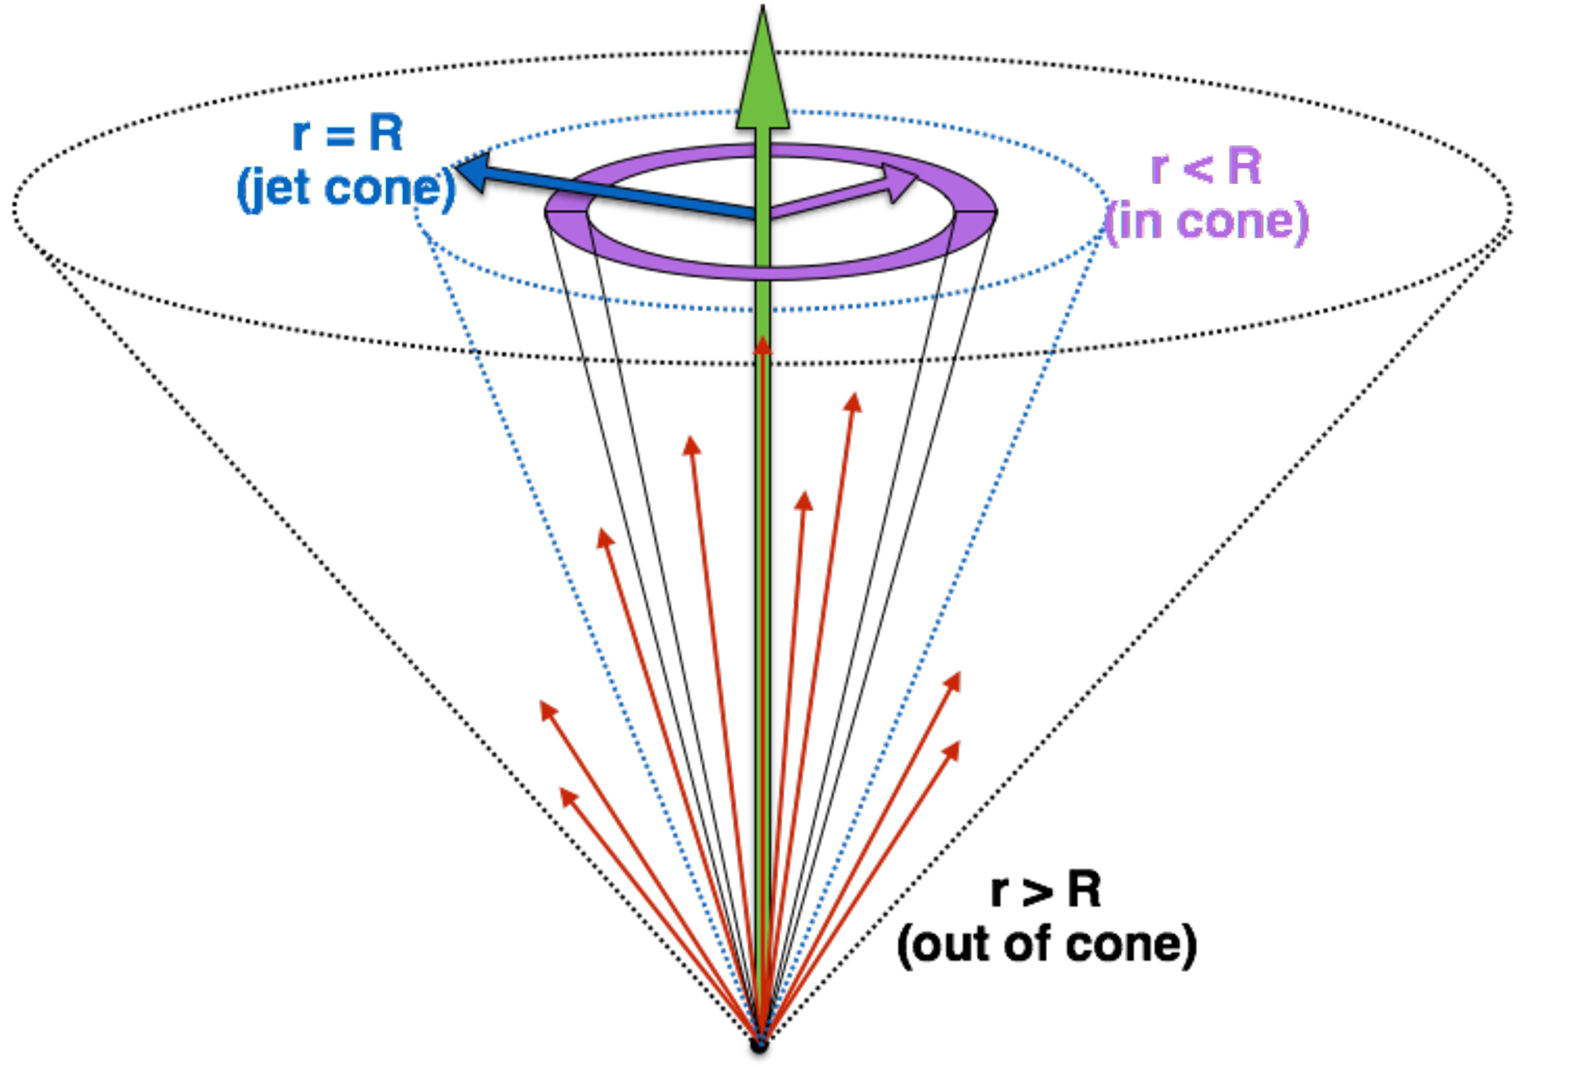
\includegraphics[width=0.55\textwidth]{figures_general/fragScheme_Shape.pdf} }
\caption{Illustration of the tracks in and around the jet. }
\label{Fig:dpt_def}
\end{figure}

%These distributions are of interest because they indicate how the energy of the jet is lost both in and outside the jet in \pbpb\ collisions. Similar measurements have been made by CMS~\cite{CMSPASHIN16020, Chatrchyan:2014ava}, and ATLAS~\cite{ATLAS502FFConf, Aaboud:2017bzv}.

The entire analysis flow of this measurement, along with the various cuts and corrections (discussed in Sec.~\ref{sec:cuts_corrections}) is shown in Fig:\ref{Fig:analysis_flow} and briefly described in the following paragraph.

\begin{figure}
\centerline{
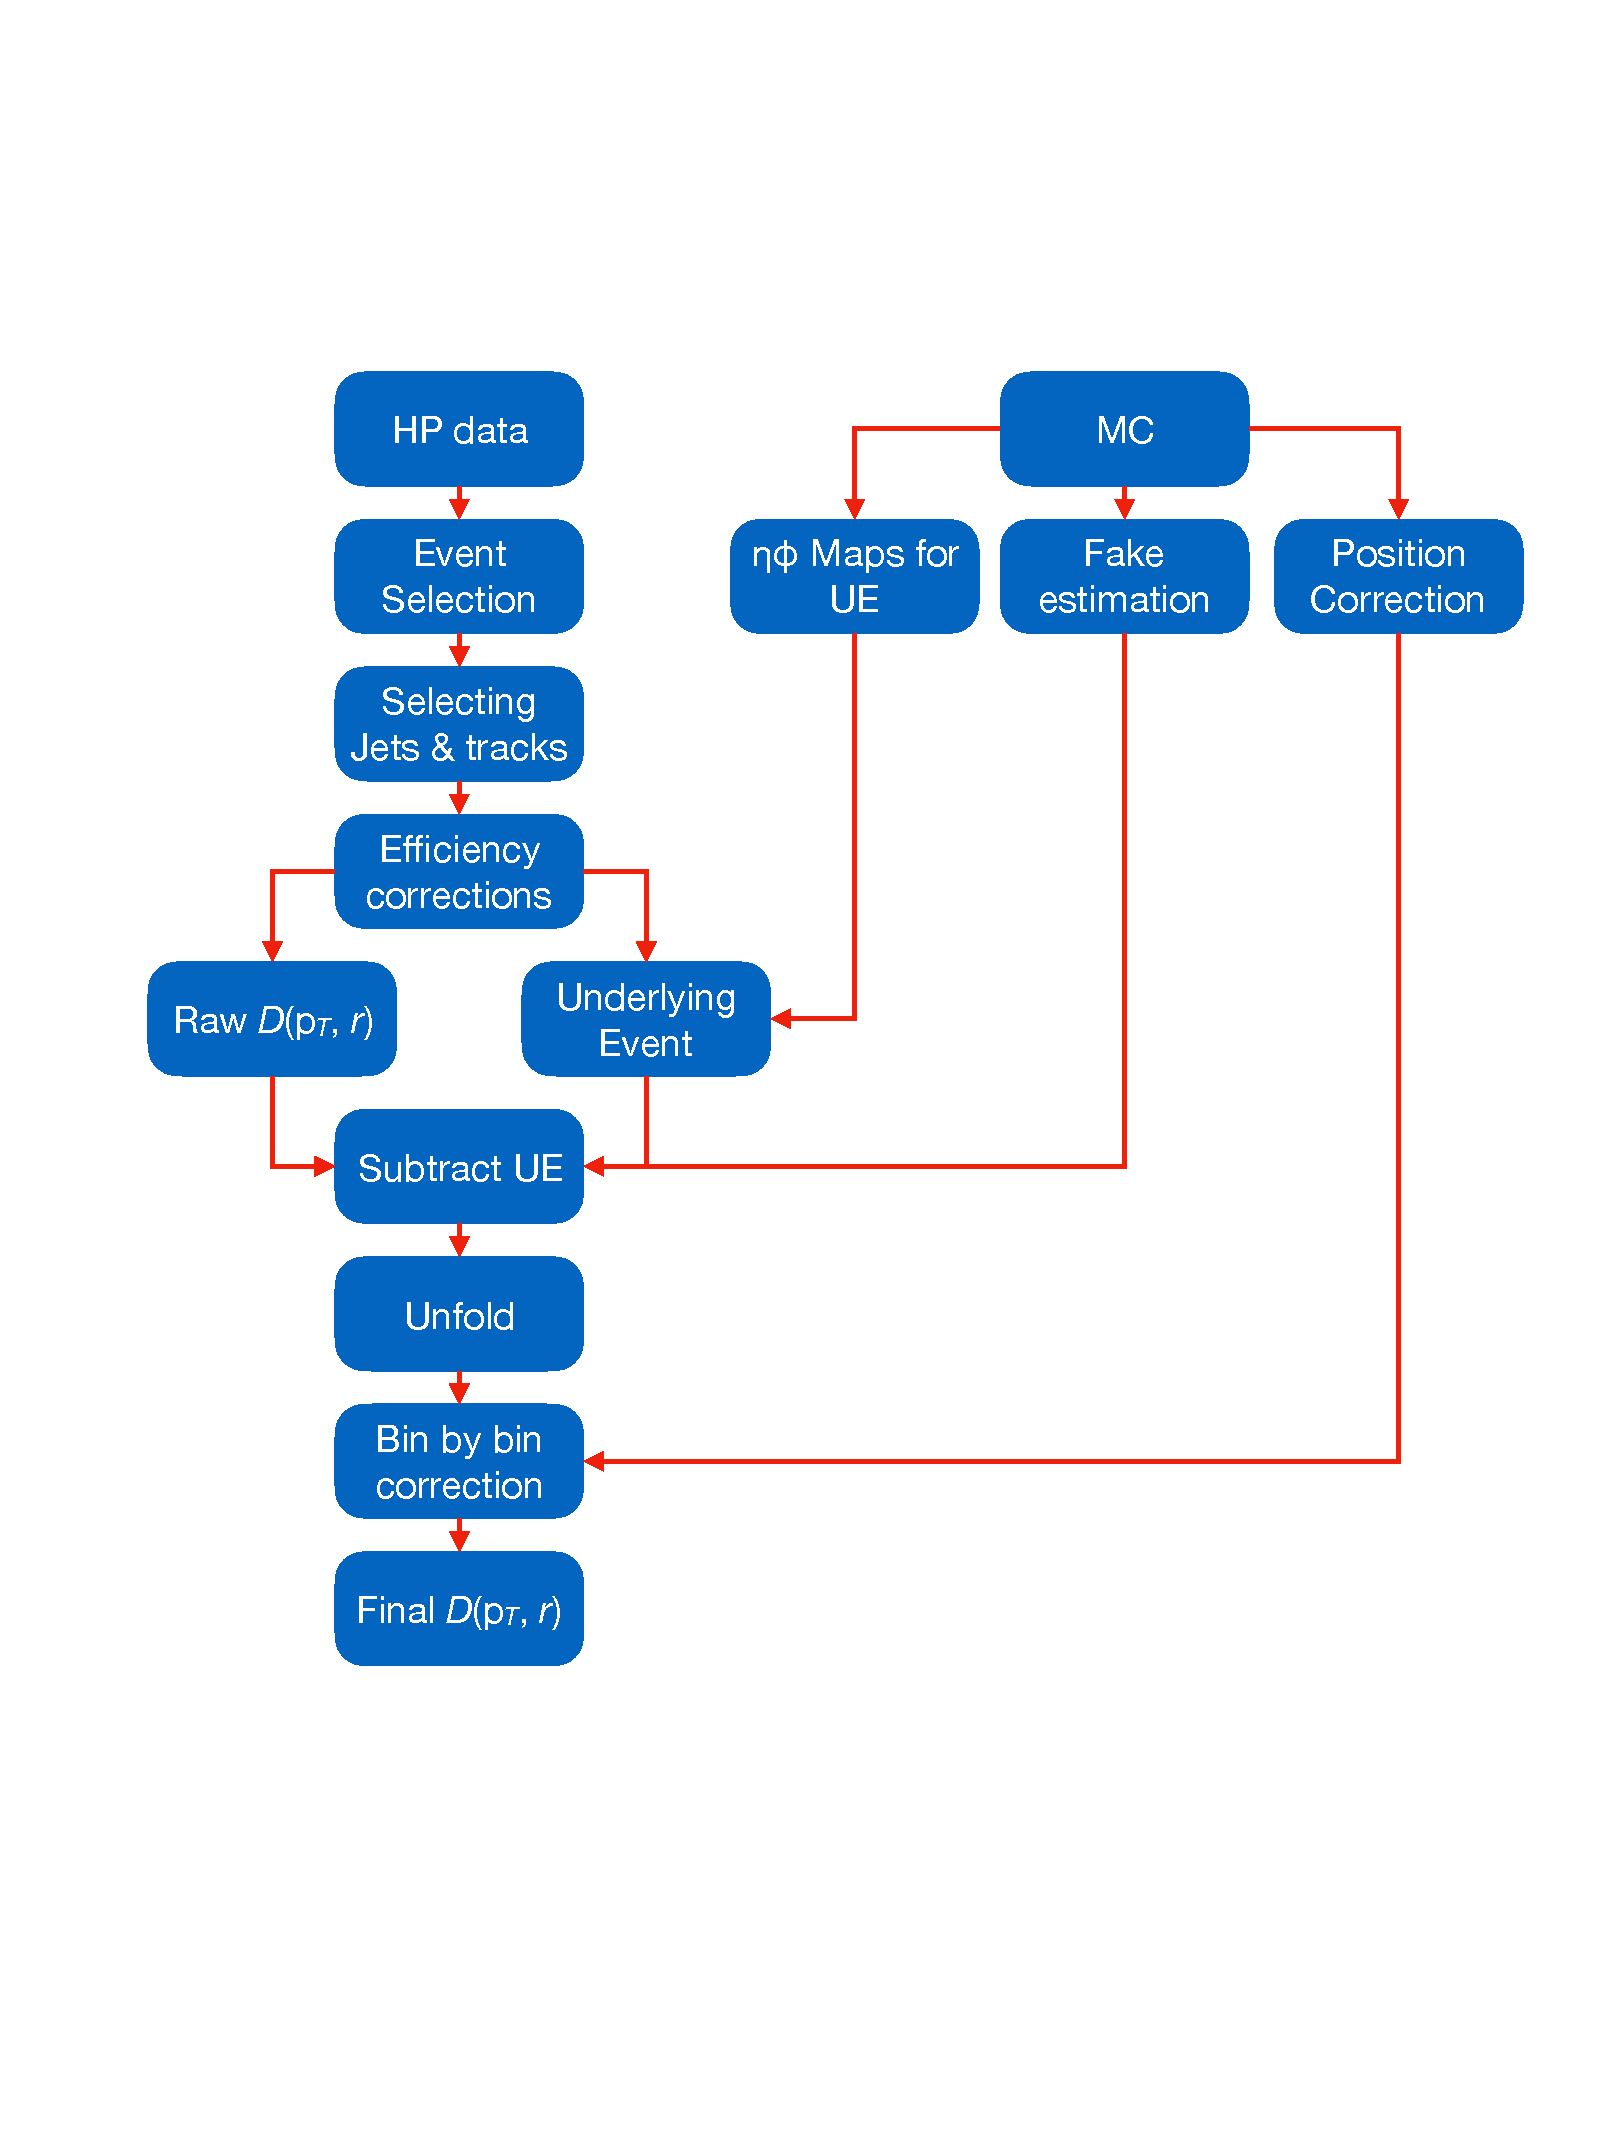
\includegraphics[width=20.cm]{figures_general/Shape_analyses_flow.pdf}
}
\caption{The diagram presents various corrections and cuts that are applied during the analysis.}
\label{Fig:analysis_flow}
\end{figure}

First, the measured charged particle yield, $\text{d}n^{\text{meas}}_{\text{ch}}/\text{d}\pTch$, within an annulus with radii $r_{\text{min}}$ and $r_{\text{max}}$ is evaluated as:
\begin{equation}
\frac{\text{d}n^{\text{meas}}_{\text{ch}}}{\text{d}\pTch} = \frac{1}{\epsilon(\pttrk, \etatrk)} \frac{\Delta N_{\text{ch}} (\pTch, r)}{\Delta \pTch}
\end{equation}

where $\Delta N_{\text{ch}} (\pTch, r)$ is the number of charged particles in a given \pTch\ range that passed the jet and track selection criteria, $r = (r_{\text{min}} + r_{\text{max}}) / 2$, and $\epsilon(\pttrk, \etatrk)$ is the charged particles reconstruction efficiency correction, applied on a track-by-track basis. In \pbpb\ collisions, the measured distributions are affected by charged particles from the underlying event, and thus need to be subtracted out (see Sec.~\ref{sec:cuts_corrections} for details):

\begin{equation}
\frac{\text{d}n^{\text{sub}}_{\text{ch}}}{\text{d}\pTch} = \frac{\text{d}n^{\text{meas}}_{\text{ch}}}{\text{d}\pTch} - \frac{\text{d}n^{\text{UE}}_{\text{ch}}}{\text{d}\pTch}
\end{equation}

The final \Dptr\ distributions are then evaluated after unfolding and normalizing with respect to the unfolded number of jets, $N_{\text{jet}}^{\text{unfolded}}$, as well as the area $A$ of the annulus at given distance $r$ :
\begin{equation}
\Dptr = \frac{1}{N_{\text{jet}}^{\text{unfolded}}} \frac{1}{\text{A}} \frac{\text{d}n^{\text{unfolded}}_{\text{ch}}}{\text{d}\pTch} \quad \quad \text{where } A = \pi (r_{\text{max}}^2 - r_{\text{min}}^2)
\end{equation}

The unfolding procedure is a combination of a two-dimensional Bayesian unfolding method in \ptjet\ and \pttrk, one-dimensional Bayesian unfolding method to correct jet spectra for the normalization and a one-dimensional bib-by-bin correction for the jet and track position resolution. 

The analysis is performed differentially in \ptjet, and centrality, with the jet \pt\ bin size growing logarithmically with \ptjet\ to ensure good statistics in the full range of the measurement. This scheme was also used in other ATLAS jet measurements~\cite{ATLAS276FFConf}. 

In order to quantify the differences between charged particle spectra in \pbpb\ and \pp\  collisions, the ratios of the charged particle spectra in \pbpb\ collisions to those in \pp\ collisions are also reported:
\begin{equation}
   R_{\Dptr} \equiv \frac{\Dptr_{\pbpb}}{\Dptr{\pp}}
\end{equation}
In the absence of modifications to the charged particle spectra in \pbpb\ collisions, both ratios will be unity.



\clearpage
%%%%%%%%%%%%%%%%%%%%%%%%%%%
\section{Input Data}
\label{sec:used_data}
% !TEX root = trackjet_intnote.tex

\subsection{Data samples}
%\label{sec:data}

This analysis used the original processing of \pp\ (reconstruction tag 7744) and \PbPb\ (reconstruction tag 7874) collisions at \sqrtsnn~=~5.02~TeV recorded in 2015 with a total integrated luminosity of 25 pb$^{-1}$ and 0.49~nb$^{-1}$ respectively. The run numbers for each set are given below:
\begin{itemize}
\item 2015 \pp\ data: 286282, 286361, 286364, 286367, 286411, 286474
\item 2015 \PbPb\ data: 286711, 286717, 286748, 286767, 286834, 286854, 286908, 286990, 287038, 287044, 287068, 287222, 287224, 287259, 287270, 287281, 287321, 287330, 287334, 287378, 287380, 287382, 287560, 287594, 287632, 287706, 287728, 287827, 287843, 287866, 287924, 287931
\end{itemize}


%\begin{itemize}
%   \item
%286711,  287068,  287560,
%286717,  287222,  287594,
%286748,  287224,  287632,
%286767,  287259,  287706,
%286834,  287270,  287728,
%286854,  287281,  287827,
%286908,  287321,  287843,
%286967,  287330,  287866,
%286990,  287334, 287924,
%286995,  287378,  287931,
%287038,  287380,
%287044,  287382
%\end{itemize}
Various hard probe triggers (high-\pT\ jets, muons, electrons, and photons) are group into a Hard Probe (HP) stream and Main stream in \PbPb\ and \pp\ data taking periods respectively. The \pp\ data samples from the Main stream used in this analysis are listed in Table~\ref{tab:events}. For the analysis of the \pbpb\ data the officially produced HION7 derivation samples from the Hard Probe stream are used. The list of datasets together with detailed description of HION7 derivation setup can be found in Ref.~\cite{HIdataderviation}. Additionally to the jet triggered data sample, \PbPb\ collisions recorded by Minimum-Bias (MB) triggers grouped in to MB stream are utilized in this analysis. The following MB data sets are used: \texttt{data15\_hi.0028*.physics\_MinBias.merge.AOD.r7874\_p2580}.



\begin{table}[h]
\begin{center}
\begin{tabular}{|c|c|c|}
\hline
description & data set names & \# runs \\ \hline
%\pp, MB &  {\tt \footnotesize data13\_2p76TeV.00219*.physics\_MinBias.merge.NTUP\_HI.f519\_m1313} & 6 \\
%2013 \pp, hard probes &  {\tt \footnotesize data13\_2p76TeV.00219*.physics\_HardProbes.merge.NTUP\_HI.f519\_m1313} 
	    & & 6 \\ \hline
2015 \pp, hard probes &  {\tt \footnotesize data15\_5TeV.periodK.physics\_Main.PhysCont.AOD.repro20\_v03} 
& 5 \\ \hline
2015 \pp, hard probes &  {\tt \footnotesize data15\_5TeV.periodVdM.physics\_Main.PhysCont.AOD.repro20\_v03} 
& 1 \\ \hline
\end{tabular}
\caption{Summary of data samples used in the \pp\ analysis.}
\label{tab:events}
\end{center}
\end{table}

\subsection{Trigger Selection}

%The data used in this study utilize the jet triggered data samples grouped into Hard Probe (HP) stream. 

To maintain efficiency for events containing hard probes specific jet triggers are used. First, events are identified at the L1 trigger by various L1 triggers. These L1 ``seeds'' are passed to the High Level Trigger (HLT) where jet trigger algorithm with various thresholds on \pT\ of the jet was used for the final selection. 

Low \pT\ HLT jet triggers in \pp\ collisions were seeded by L1 MB random trigger ($\texttt{L1RD0}$) or L1 triggers requiring different thresholds on total energy in the calorimeter ($\texttt{L1TE}$). High \pT\ HLT jet triggers in \pp\ collisions were seeded by different L1 jet triggers performing a simple sliding window algorithm to find jet candidates ($\texttt{L1J}$). In \PbPb\ collisions, L1 total energy triggers were used to seed all HLT jet trigger chains.

We analyze jets selected from jet triggers in the region of jet \pt\ for which the triggers are fully efficient\footnote{Efficiency is better than 99\%} for jets. Since the analysis only used jets above 100 GeV, the appropriate triggers were selected. For \pp, only the {\footnotesize{HLT\_j85}} trigger (fully efficient above 88.8 GeV) was used. For \pbpb\, the only trigger used was the {\footnotesize{HLT\_j75\_ion\_L1TE50}} (fully efficient above 91 GeV).
   
  The performance of the jet trigger in 2015 is described in~\cite{HITMF} and the trigger efficiency is presented in Figure~\ref{Fig:Trigger_pp5} (\pp\ collisions) and Figure~\ref{fig:Trigger_PbPb} (\pbpb\ collisions). The trigger efficiency for two low thresholds is evaluated using MB events. The low \pT\ thresholds are used as the reference to evaluate the performance at higher \pT. The efficiency for the higher threshold is bootstraped from lower thresholds. The broader turn-on of the jet trigger in \pbpb\ compared to \pp\ collisions is caused by significant differences between the HI jet trigger reconstruction algorithm used at the time of the data taking and the current version of the offline reconstruction software.

  \begin{figure}[h]
 \centerline{
 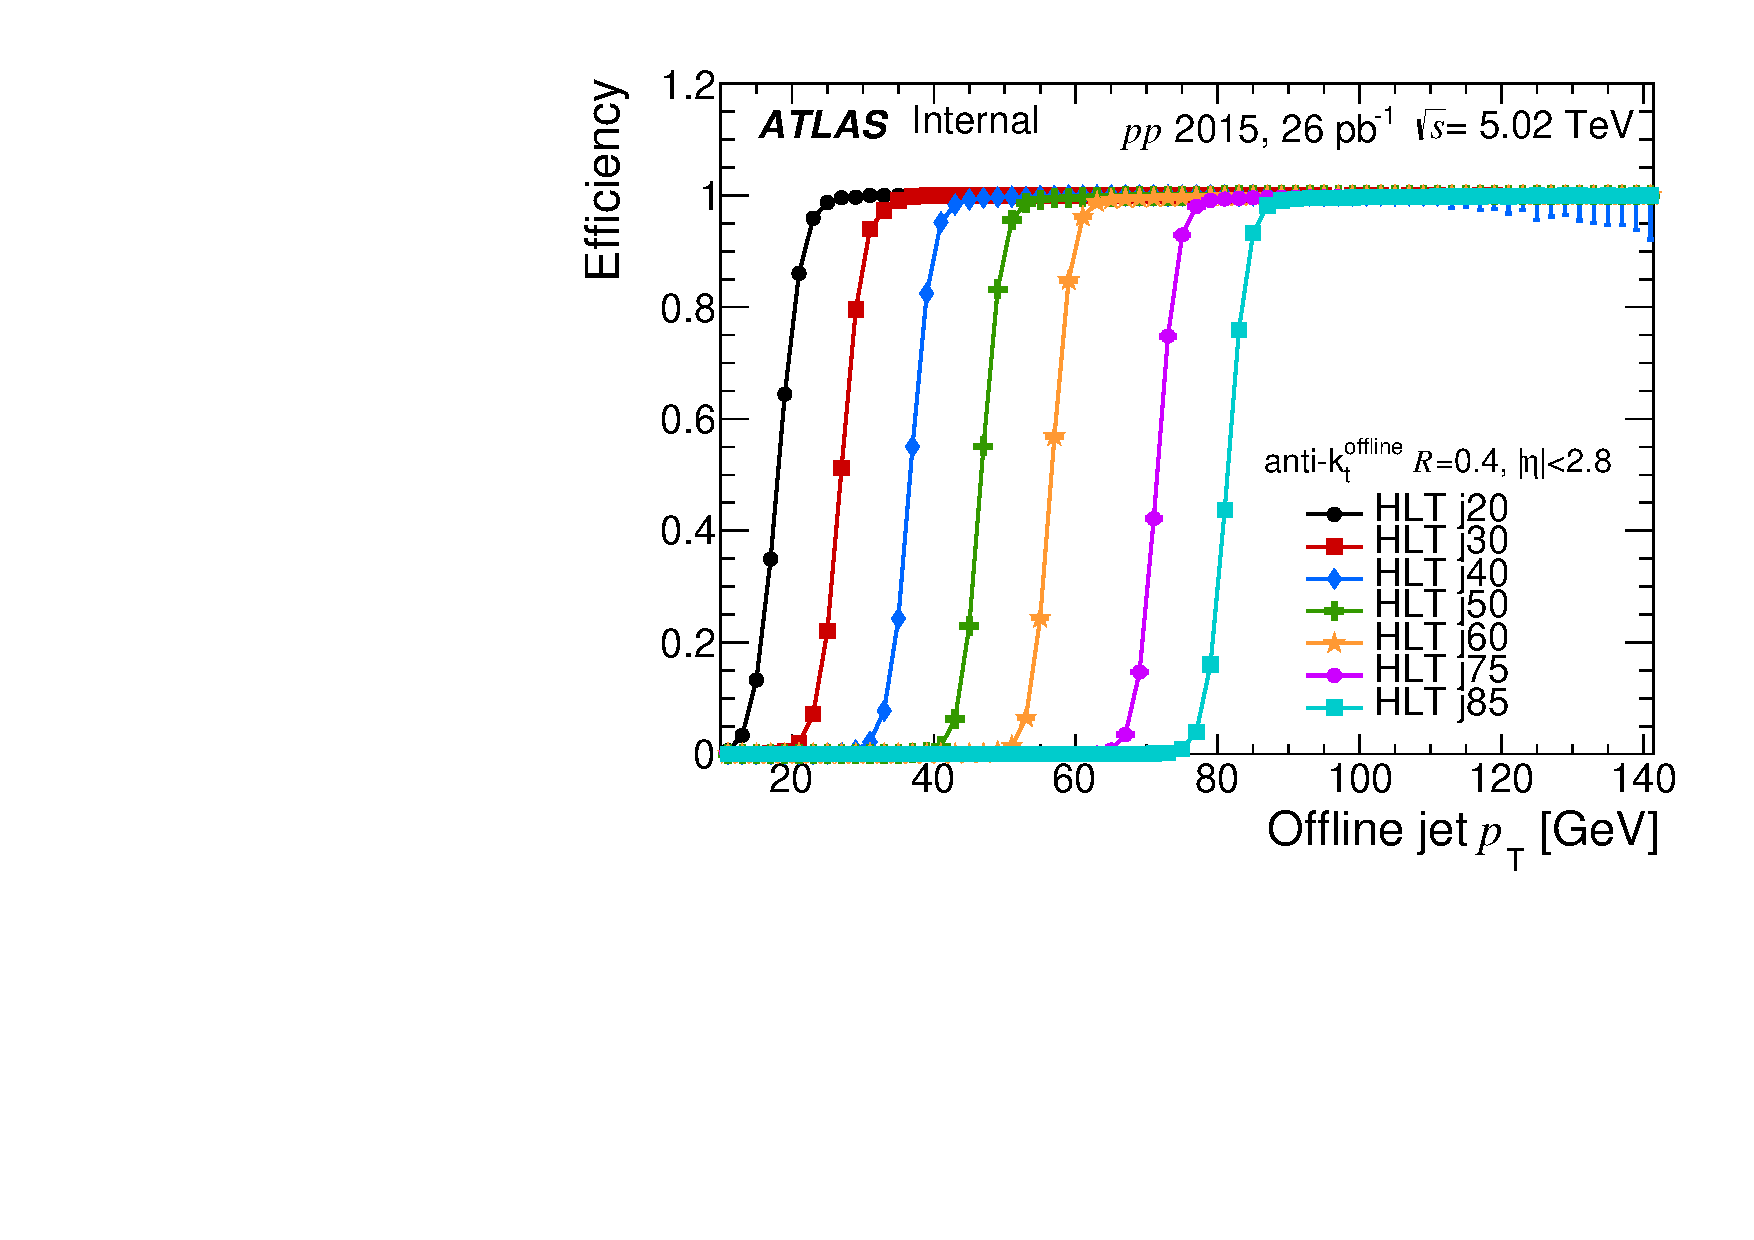
\includegraphics[width=0.75\textwidth]{figures_general/Eff_pp_5TeV_central.pdf}
}
 \caption{Trigger efficiencies for R=0.4 offline jets for seven HLT jet triggers in \pp\ collisions at 5.02 TeV.}
 \label{Fig:Trigger_pp5}
 \end{figure}


 \begin{figure}[h]
    \centerline{
       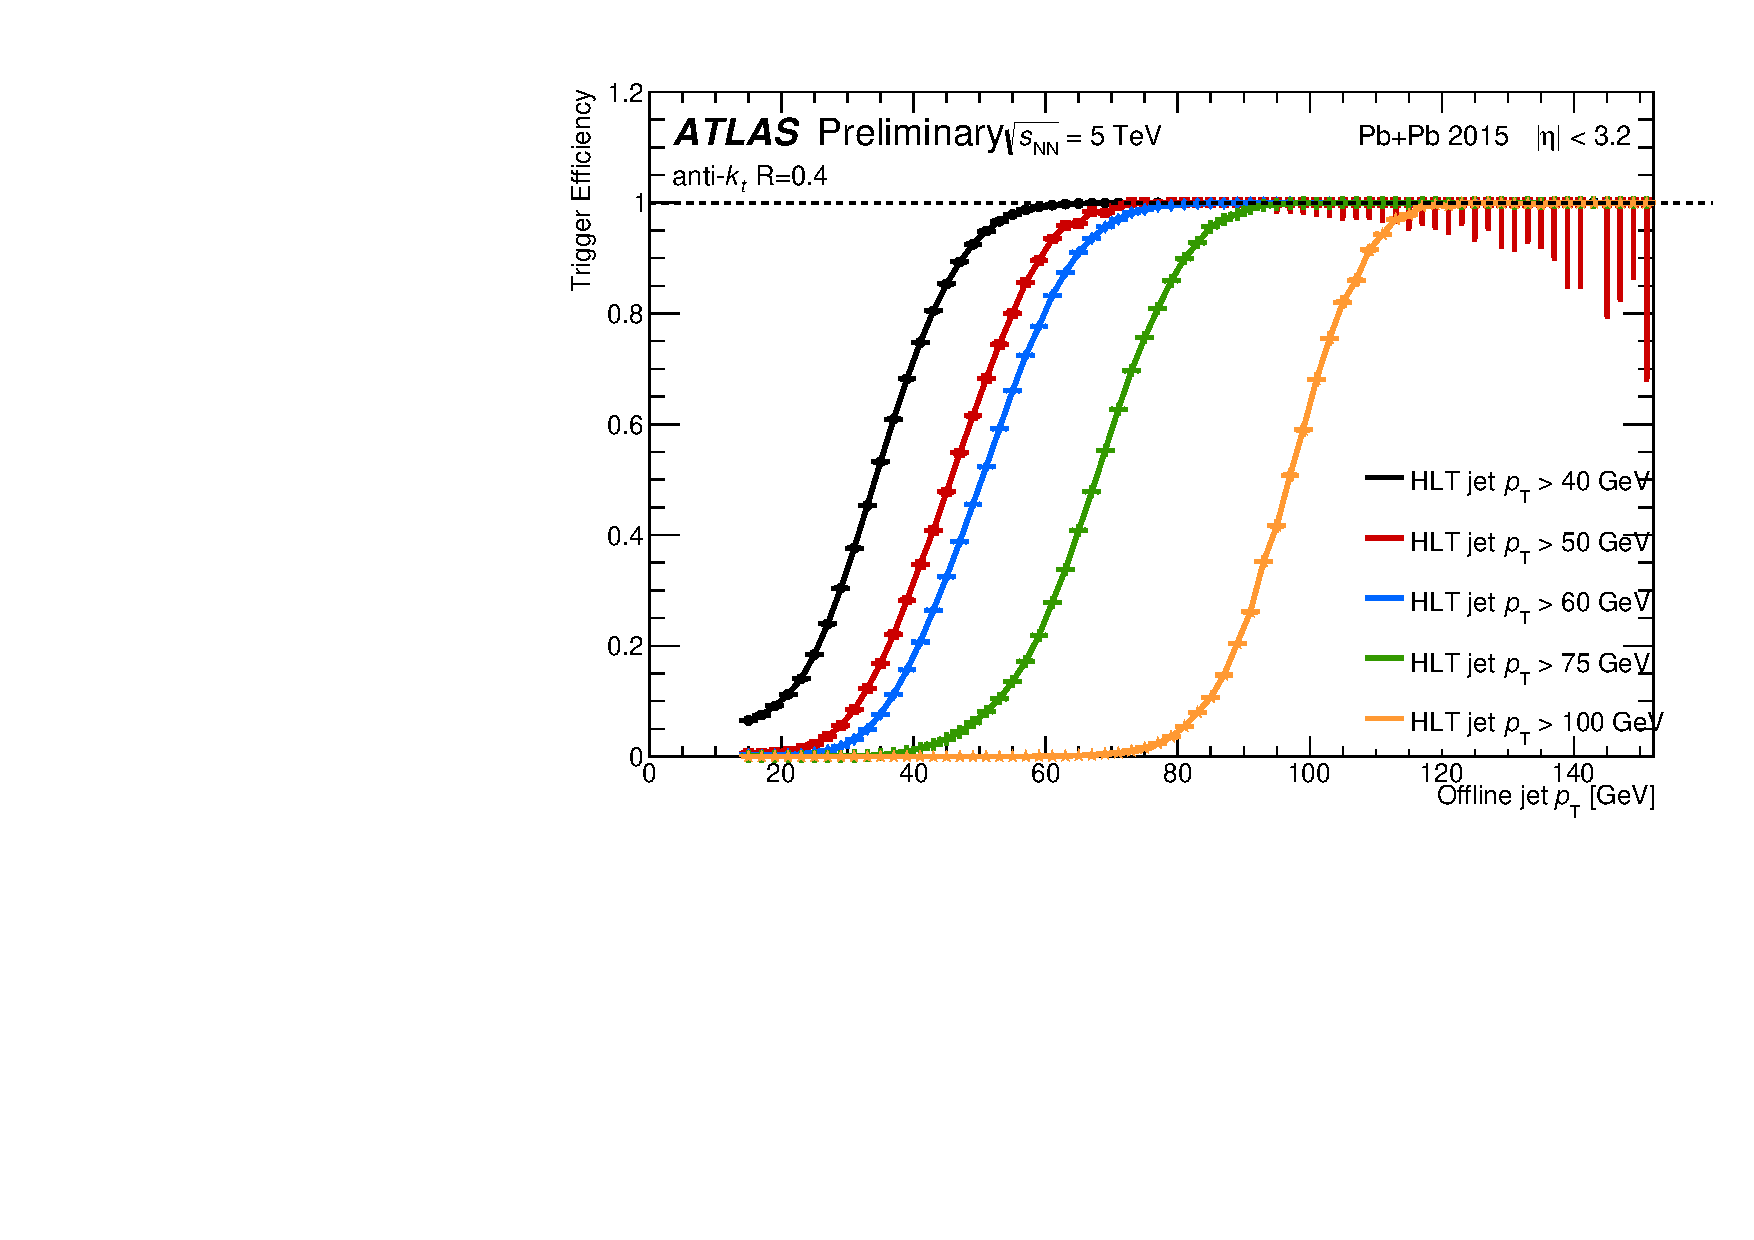
\includegraphics[width=0.75\textwidth]{figures_general/trigger_eff_PbPb_CentInclusive.pdf}
    }
    \caption{Jet trigger efficiency in centrality inclusive (0-80\%) \pbpb\ collisions for R=0.4 offline
    jets.}
    \label{fig:Trigger_PbPb}
 \end{figure}

In addition to the jet triggered sample, a MB triggered sample defined by a logical OR of the total energy trigger with a threshold of 50~\GeV\ and the ZDC coincidence trigger was used as part of the MC overlay procedure

The event fraction as a function of run number for both the hard probes stream and the minimum bias overlay stream in \pbpb\ is shown in Fig.~\ref{fig:evnt_fraction}

 \begin{figure}[h]
    \centerline{
       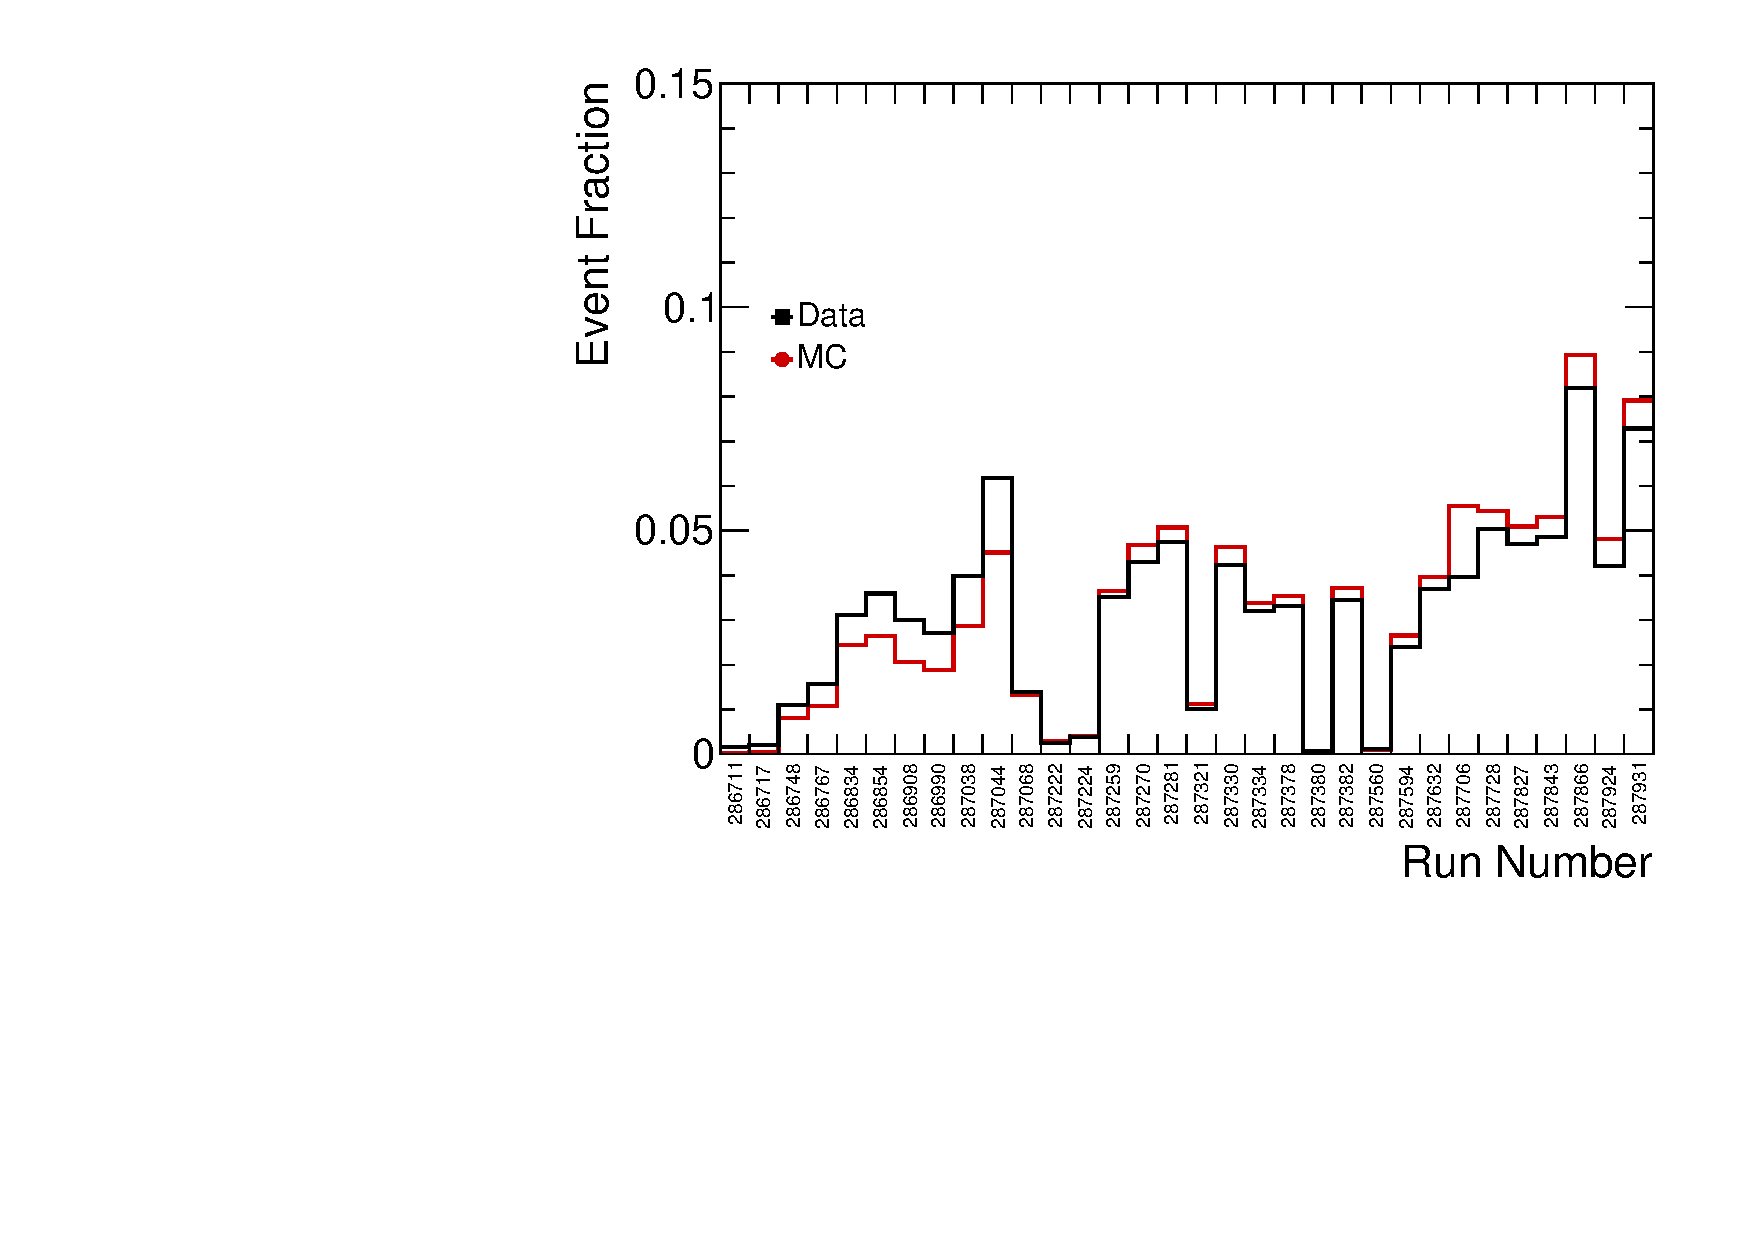
\includegraphics[width=0.9\textwidth]{figures_general/EventPercentages.pdf}
    }
    \caption{Event fraction as a function of runs for Hard Probes and the Minimum Bias Overlay Streams in \pbpb\ collisions.}
    \label{fig:evnt_fraction}
 \end{figure}

The run dependence of the underlying event (a core part of this measurement) was tested by dividing the data and MC into three periods with approximately equal number of events in each period: 286711 -- 287259, 287270 -- 287632, and 287706 -- 287931. The underlying event determined for each period compared to the nominal underlying event evaluated for the entire dataset is shown in Fig.\ref{fig:weighted_runs}, and it can be seen that the UE is stable throughout the data taking period.
%The systematic uncertainty associated with the run dependence was included in the calculation of the systematic uncertainty on the result.

 \begin{figure}[h]
    \centerline{
       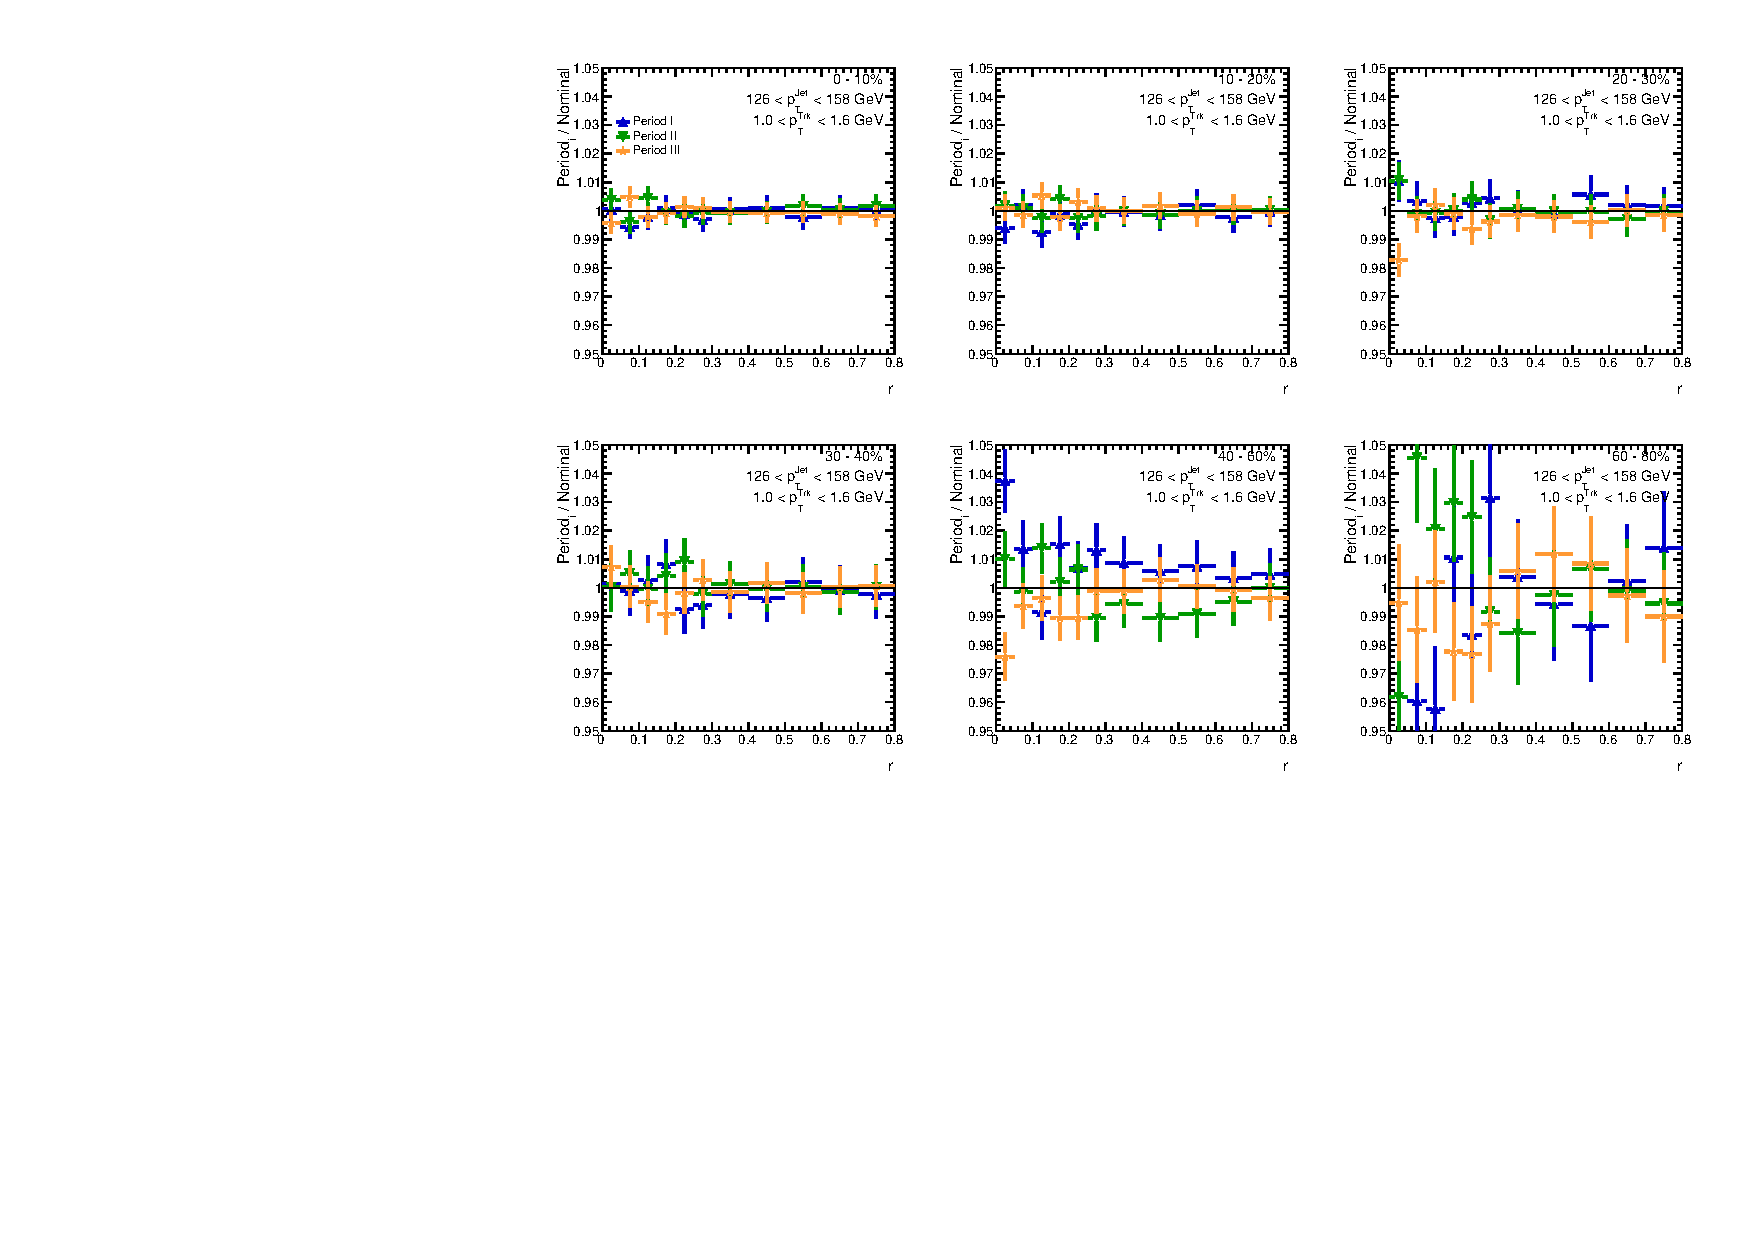
\includegraphics[width=0.75\textwidth]{figures_general/weightedRuns.pdf}
    }
    \caption{Stability of the underlying event for three different periods of the data taking. The different curves indicate the ratio of the underlying event in each period of data taking to the underlying event determined in the entire dataset.}
    \label{fig:weighted_runs}
 \end{figure}



% two separate MB data sample are used: 1) to estimate the underlying event contribution of charged particles to measured distributions; 2) to study detector performance in conditions that match the data. The first sample was recorded by MB triggers requiring either to have the transverse energy in the whole calorimeter exceeding 50 GeV at the Level-1 trigger (HLT\_noalg\_mb\_L1TE50) or to have a track reconstructed in the inner detector in coincidence with ZDC signals on both sides (HLT\_mb\_sptrk\_ion\_L1ZDC\_A\_C\_VTE50). The second sample was recorded with the MB trigger defined by a logical OR of the total energy trigger with a threshold of 50~\GeV\ and the ZDC coincidence trigger. This sample was used because it was utilized in the MC overlay procedure. Furthermore, two total transverse-energy triggers requiring 1.5~\TeV\ and 6.5~\TeV\ were used to enhance higher multiplicity events.

%
%   \begin{table}[h]
%\centering
%\begin{tabular}{|c|c|}
%\hline
%trigger & \ptjet (GeV) \\
%\hline
%%{\tt \footnotesize EF\_j20} & 25.7-35.2\\
%%{\tt \footnotesize EF\_j30\_L1TE5} & 35.2-43.6\\
%%{\tt \footnotesize EF\_j40\_L1TE5}  & 43.6-52.8\\
%%{\tt \footnotesize EF\_j50\_L1J12} & 52.8-62.5\\
%%{\tt \footnotesize EF\_j60\_L1J15} & 62.5-78.8\\
%%{\tt \footnotesize EF\_j75\_L1J20} & 78.8-88.8\\
%{\tt \footnotesize EF\_j85} & $>$~88.8\\
%\hline
%\end{tabular}
%\caption{Triggers used in the analysis of 2015 \pp\ data and the corresponding \ptjet\ ranges.}
%\label{tab:jettrigpp5}
%\end{table}
%
%\begin{table}
%\centering
%\begin{tabular}{|c|c|}
%\hline
%trigger & \ptjet (GeV) \\
%\hline
%{\tt \footnotesize EF\_j75\_ion\_L1TE50} & $>$~91\\
%%{\tt \footnotesize EF\_j100\_ion\_LITE50} & $>$~114\\
%\hline
%\end{tabular}
%\caption{Triggers used in the analysis of 2015 \pbpb\ data and the corresponding \ptjet\ ranges.}
%\label{tab:jettrigpbpb5}
%\end{table}


\subsection{Monte Carlo Samples}
%The studies in this note utilize high-statistic MC samples that are used to study the performance of the analyses and in the unfolding procedure. The MC12 PYTHIA6.4 \pp\ di-jet events at $\sqrt{s} =5.02$~TeV with the same rapidity shift in the center of mass as in the data, were embedded on top of heavy ion MB data events collected during the 2013 run using a MB trigger in \texttt{MinBiasOverlay} stream. The \texttt{MinBiasOverlay} records the data without zero suppression. The signal from this trigger was combined with the signal from PYTHIA6.4 at the digitization stage and then reconstructed as a combined event. MC samples are used for both the period A and period B running conditions. Truth jets with \pTtrue\ were defined in the MC sample as the output of the \antikt\ algorithm with \RFour\ applied to the final-state particles generated by PYTHIA6.4.

 

This analysis also utilizes MC15 \pythiaeight\ \pp\ jet events at $\sqrt{s} =5.02$~TeV with the A14 ATLAS tune and the NNPDF23LO pdfs~\cite{ATL-PHYS-PUB-2014-021}. The definitions of the \pp\ MC samples can be found in Tab.~\ref{Tab:MCSamples_pp5}. The \pbpb\ MC uses POWHEG+\pythiaeight\ events that are overlayed on top of MB \PbPb\ collisions.  
These samples are listed in Tab.~\ref{tab:overlay}. 

\begin{table}[htbp]
\centering
\begin{tabular}{|l|p{0.65\linewidth}|}
\hline
\multicolumn{1}{|c|}{JZ} & \multicolumn{1}{c|}{Dataset Name}                 		                                  \tabularnewline \hline
2	& {\tt \footnotesize mc15\_5TeV.420022.PowhegPythia8EvtGen\_A14\_NNPDF23LO\_CT10ME\_ jetjet\_JZ2R04.merge.DAOD\_HION7.e4109\_s2860\_r7792\_r7676\_p3442}                                                     \tabularnewline \hline
3	& {\tt \footnotesize mc15\_5TeV.420023.PowhegPythia8EvtGen\_A14\_NNPDF23LO\_CT10ME\_ jetjet\_JZ3R04.merge.DAOD\_HION7.e5067\_s2860\_r7792\_r7676\_p3442}                                                                                  \tabularnewline \hline
4	& {\tt \footnotesize mc15\_5TeV.420024.PowhegPythia8EvtGen\_A14\_NNPDF23LO\_CT10ME\_ jetjet\_JZ4R04.merge.DAOD\_HION7.e5067\_s2860\_r7792\_r7676\_p3442}                                                                   \tabularnewline \hline
\end{tabular}
\begin{tabular}{| c | c | c | c | c |} \hline
J & \RFour\ \pTtrue\ [\GeV]  & $\sigma$ [$\mathrm{nb}$] $\times$ $\epsilon$ & $\#$events \\ \hline
2  & 60--160 &  (6.4 $\times$ 10$^5$) $\times$ (4.27 $\times$ 10$^{-3}$) & 5.8 M \\ \hline
3  & 160--400 &  (4.7 $\times$ 10$^3$) $\times$ (5.28 $\times$ 10$^{-3}$) & 5.9 M \\ \hline
4  & 400--800 &  (2.7 $\times$ 10$^1$)  $\times$ (4.58 $\times$ 10$^{-3}$) & 5.8 M \\ \hline
\end{tabular}
\caption{5.02 TeV \pythiaeight\ \pp\ MC samples.}
\label{Tab:MCSamples_pp5}
\end{table}


\begin{table}[htbp]
\centering
\begin{tabular}{|l|p{0.65\linewidth}|}
\hline
\multicolumn{1}{|c|}{JZ} & \multicolumn{1}{c|}{Dataset Name}                 		                                  \tabularnewline \hline
2	& {\tt \footnotesize mc15\_5TeV.420022.PowhegPythia8EvtGen\_A14\_NNPDF23LO\_CT10ME\_jetjet \_JZ2R04.merge.DAOD\_HION7.e4109\_d1421\_r8238\_r8052\_p3196}                                                     \tabularnewline \hline
3	& {\tt \footnotesize mc15\_5TeV.420023.PowhegPythia8EvtGen\_A14\_NNPDF23LO\_CT10ME\_jetjet \_JZ3R04.merge.DAOD\_HION7.e4109\_d1421\_r8238\_r8052\_p3196}                                                                                  \tabularnewline \hline
4	& {\tt \footnotesize mc15\_5TeV.420024.PowhegPythia8EvtGen\_A14\_NNPDF23LO\_CT10ME\_jetjet \_JZ4R04.merge.DAOD\_HION7.e4109\_d1421\_r8238\_r8052\_p3196}                                                                   \tabularnewline \hline
\end{tabular}
\caption{\pbpb\ data overlay datasets used here.}
\label{tab:overlay}
\end{table}

\clearpage

%\clearpage
%%%%%%%%%%%%%%%%%%%%%%%%%%%
\section{Event Selection }
\label{sec:event_selection}
% !TEX root = trackjet_intnote.tex

The standard ATLAS event quality requirements were applied for the event selection both for the \pp\ and \PbPb\ event selection.
\begin{itemize}
\item All the sub-detector systems were required to be fully functional: all the data were required to pass the official good run list:
 \\ $\texttt{\scriptsize data15\_5TeV.periodAllYear\_DetStatus-v75-repro20-01\_DQDefects-00-02-02\_PHYS\_HeavyIonP\_All\_Good.xml}$ (2015 \pp) 
 \\ $\texttt{\scriptsize data15\_5TeV.periodVdM\_DetStatus-v75-repro20-01\_DQDefects-00-02-02\_PHYS\_HeavyIonP\_All\_Good.xml}$ (2015, VdM \pp)
 \\ $\texttt{\scriptsize data15\_hi.periodAllYear\_DetStatus-v75-repro20-01\_DQDefects-00-02-02\_PHYS\_HeavyIonP\_All\_Good.xml } $ (2015 \pbpb).

\item All events are required to have a good reconstructed primary vertex.
\item The primary vertex must be within 150~mm from the center of ATLAS detector, as a fiducial tracking region.
 
\item Additional event cleaning to remove additional detector imperfections as described here~\cite{2015EventCleaning} is used. 
\item In \PbPb\ collisions the pileup contribution is removed using the  $\texttt{HIAnalysisTools}$ \cite{HIAnalysisTools}. 
\end{itemize}


Figures~\ref{Fig:EventCounts} presents the total number of \pp\ and \pbpb\ events, respectively, entering the analysis together with rejection power of various event quality cuts. A slightly higher fraction of empty events without primary vertex is observed in pp collisions. Some of these events are rejected by multiple cuts. ``Rejection by centrality'' indicates the number of event in HP stream that is outside the 0-80\% centrality bin.

\begin{figure}
\centerline{
\begin{tabular}{cc}
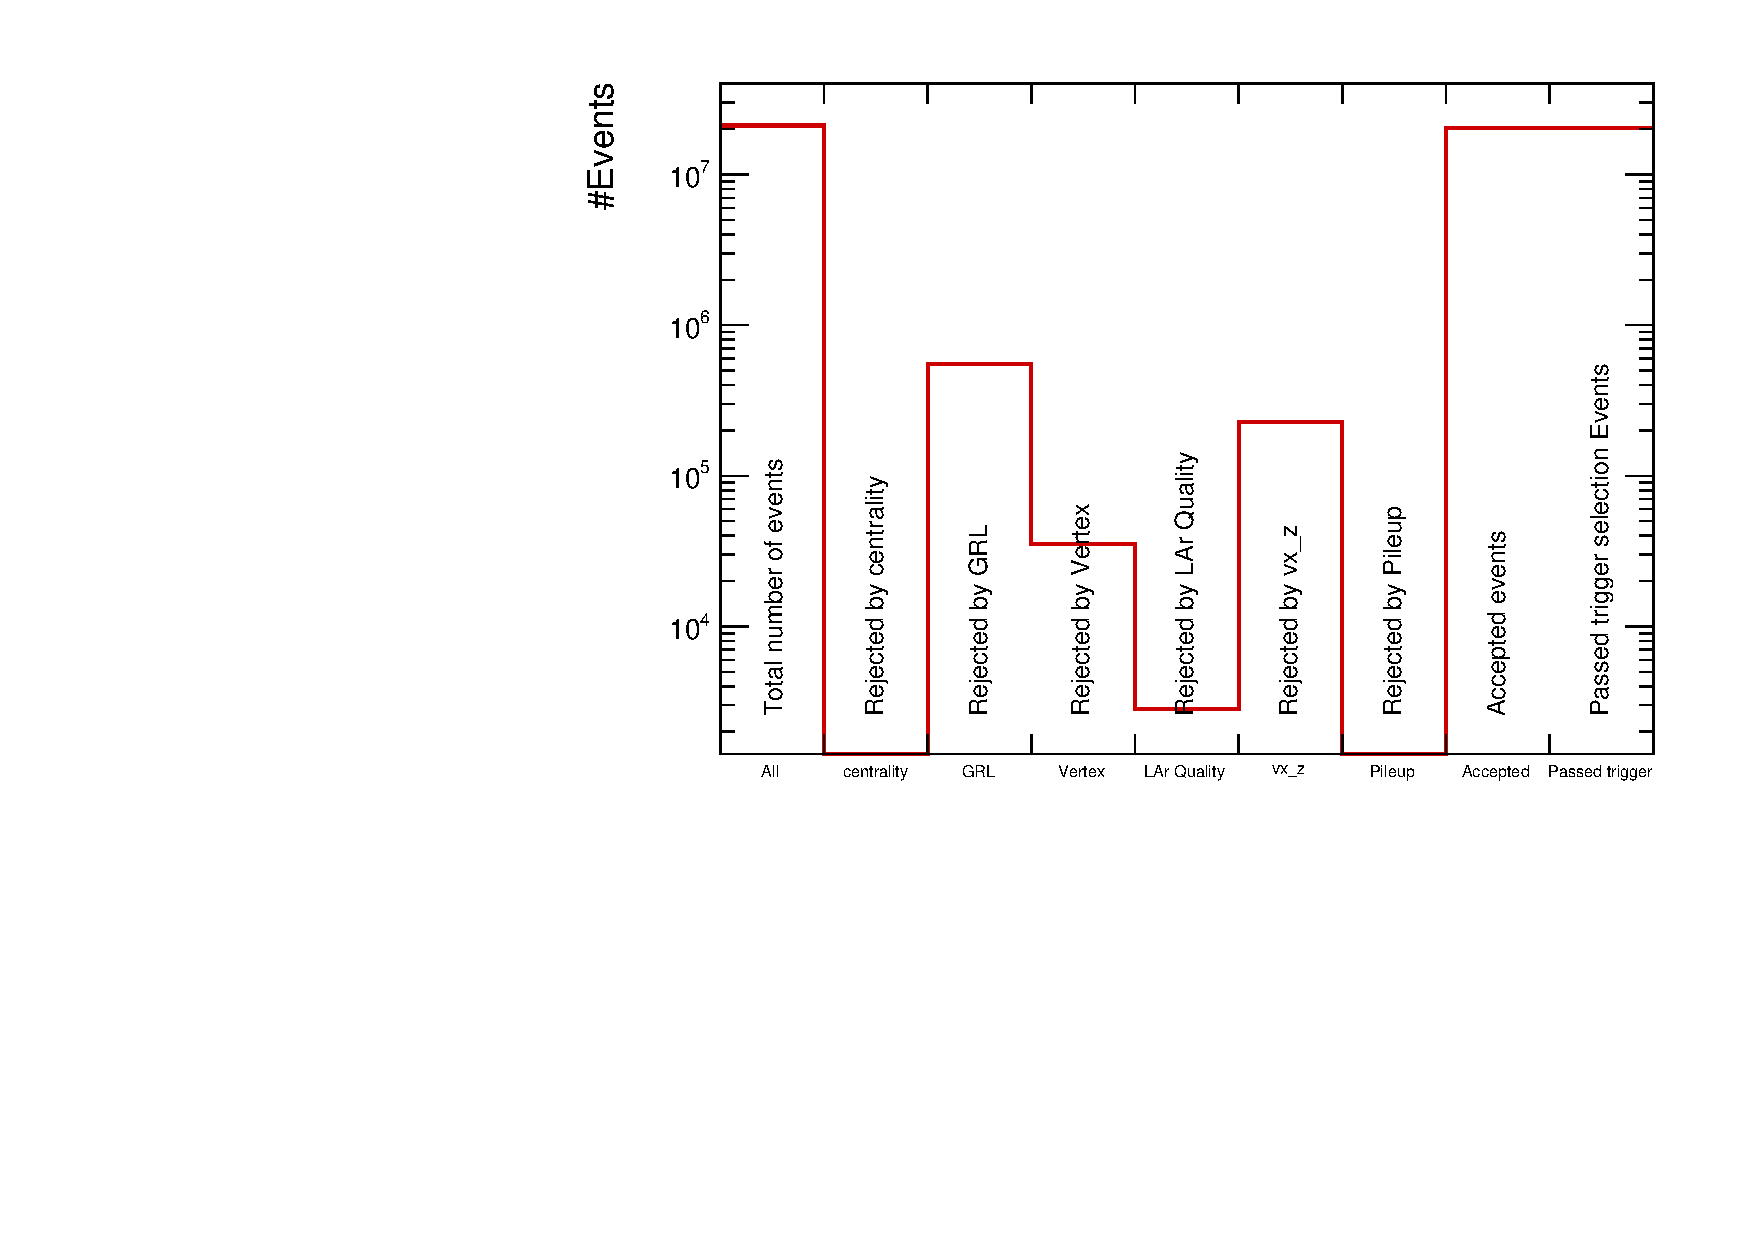
\includegraphics[width=0.45\textwidth]{figures_general/EventAccept_pp.pdf} & 
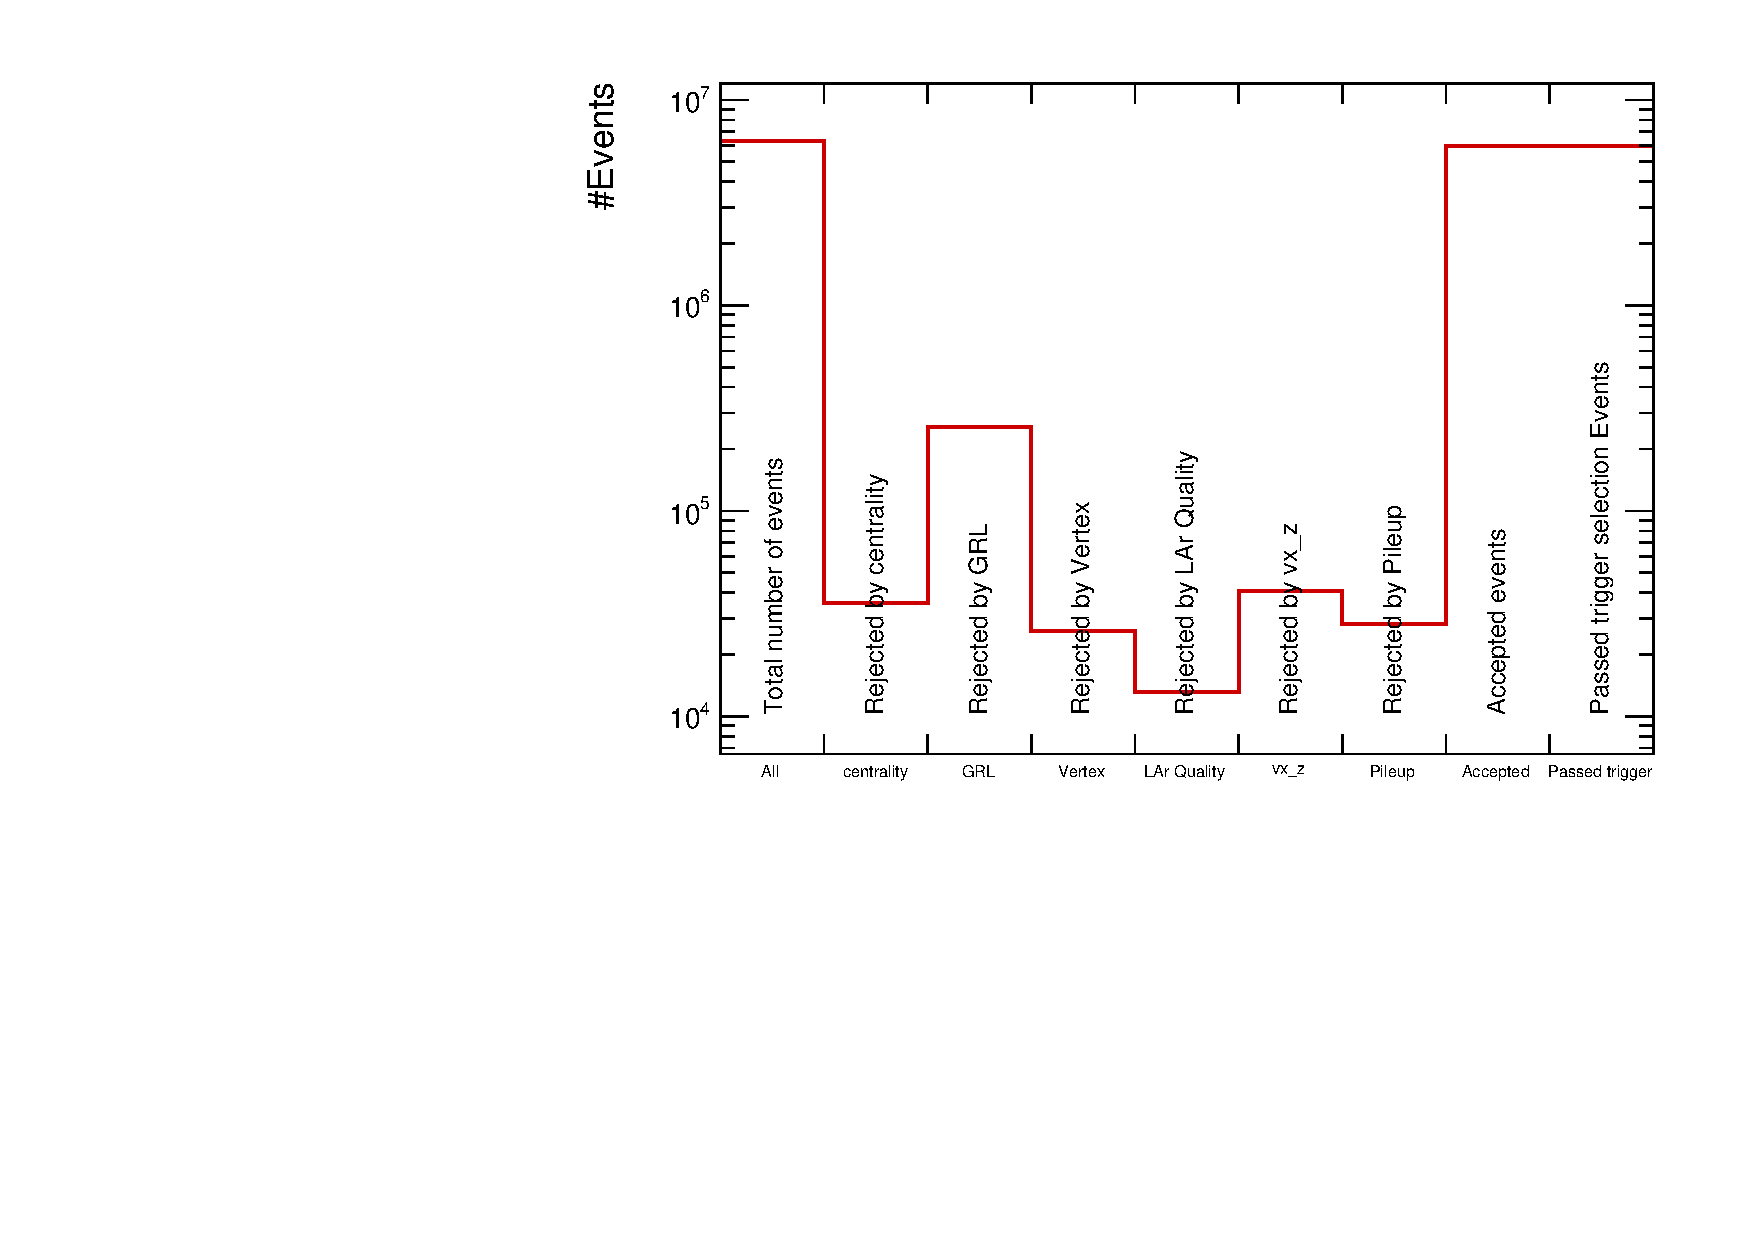
\includegraphics[width=0.45\textwidth]{figures_general/EventAccept_PbPb.pdf}
\end{tabular}}
\caption{
The number of 2015 \pp\  (left) and \PbPb\ (right) events used and rejected by various event quality cuts. }
\label{Fig:EventCounts}
\end{figure}


\subsection{Centrality Selection}
\label{sec:cent}

The centrality of the collision is a degree of the overlap of two colliding nuclei that can be quantified by the impact parameter that is the distance between the centers of the two nuclei. If they collide head on the collision is central, if they just graze each other we speak about peripheral collisions. We cannot measure the impact parameter to determine the centrality, but we can measure the overall event activity in the collision, characterized e.g. by the sum of \Et\ measured in FCal calorimeters on both sites. Central collisions have large \Et\ deposits in the FCal, peripheral have small \Et\ deposits.

In this analysis, The \ETfcal\ distribution is divided into percentiles of the total inelastic cross section for \PbPb\ collisions. The first percentile, $0-10\%$, represents the $10\%$ of collisions with the largest event activity, smallest impact parameter. The last percentile, $90-100\%$, represents the $10\%$ of collisions where there is the smallest event activity and largest impact parameter. 
Seven centrality classes have been used: 0-10\%, 10-20\%, 20-30\%, 30-40\%, 40-60\%, 60-80\%. 
The most peripheral collisions 80-100\%, are excluded due to  the small number of jets.
The centrality selections are documented in Ref.~\cite{ref:centrality}. The \PbPb\ MC is re-weighted in the way that it has the same centrality distribution as the jet triggered data sample.

\clearpage

\clearpage
\section{Jet Reconstruction}
\label{sec:reconstruction}
% !TEX root = trackjet_intnote.tex

\label{Sec:JetRec}
For the measurement presented here, we use the jets reconstructed in the calorimeter 
using the \antikt\ algorithm \cite{Cacciari:2008gp} with \RFour.
The underlying event (UE) contribution to jets is subtracted on 
an event by event basis at the cell level. The details on the jet reconstruction 
procedure and performance in heavy ion collisions have been described in 
\cite{ATLAS-COM-PHYS-2011-1733}, here we will only shortly summarize the main 
features of the heavy ion jet reconstruction.

In order to reconstruct jets in heavy ion collisions, a large background from 
the UE has to be subtracted from each jet. 
The UE subtraction procedure is done in several iterative steps. 
First an estimate of the UE average transverse energy density, $\rho_i(\eta)$, 
is evaluated for each calorimeter layer $i$ in intervals of $\eta$ of width 
$\Delta \eta = 0.1$ using all cells in each calorimeter layer, within a given 
$\eta$ interval excluding those within $\Delta R < 0.4$ of ``seed'' jets. In the first 
subtraction step, the ``seed'' jets are defined to be jets reconstructed using the 
\antikt\ algorithm with \RTwo\ jets which have at 
least one tower  (a tower is a 0.1x0.1 region of the calorimeter and the energy
associated with it is the sum of the energies from all contributing calorimeter layers
in that region)
with $\Et > 3$~GeV and which have a ratio of the maximum to 
the mean tower associated with the jet of at least 4. 
  The UE-subtracted cell energies  were calculated according to:
\begin{equation}
\label{eqn:UE}
E_{\mathrm{T},i}(\eta, \phi)^{\mathrm{sub}} = E_{\mathrm{T},i}(\eta, \phi) - A_i \times \rho_i(\eta) 
\end{equation}
where $E_{\mathrm{T},i}$, $\eta$, $\phi$,  and $A_i$ represent the $\Et$, $\eta$, 
$\phi$, and area of the cell in the layer $i$. The $\rho_i(\eta)$ is the energy density per unit area in the layer $i$. The kinematics for \RTwo\ jets 
generated in this first subtraction step were calculated via a four-vector sum 
of all (assumed massless) cells contained within the jets using the \Et\ values 
obtained from Eq.~\ref{eqn:UE}.

The second subtraction step starts with the definition of a new set of 
seeds using a list of \RTwo\ calorimeter jets from the first 
subtraction step, each with $\Et > 4$~GeV. Using this new set of 
seeds, a new estimate of the UE, $\rho'_i(\eta)$, was calculated excluding 
cells within $\Delta R < 0.4$ of the new ``seed'' jets, where $\Delta R = \sqrt{ 
(\eta_{\mathrm{cell}} - \eta_{\mathrm{jet}})^2 + (\phi_{\mathrm{cell}} - \phi_{\mathrm{jet}})^2}$.


The jet energy scale calibration is based on the numerical inversion method and provides calibration constants for all jet collections used in this study~\cite{CalibrationTwiki}. The final jet energy calibration using in-situ studies is applied in the offline analysis and it is described in Sec~\ref{Sec:JetSelection}.   



Similarly, the jet reconstruction performance in 5.02 TeV \pp\ collisions was evaluated using corresponding MC samples with a full detector simulation. The jet reconstruction efficiency, JES (in this case evaluated as $\langle (\ETreco)\rangle/\ETtrue$), and JER for \pp\ collisions is shown in Fig.~\ref{Fig:Performancepp5} for \RFour\ jet.
For \pbpb\ collisions the JES is shown in Fig.~\ref{Fig:PerformancepbpbJES} and the JER is shown
in Figure~\ref{Fig:PerformancepbpbJER}.  Further studies of the jet performance in the 2015 \pbpb\
data are found in Ref.~\cite{PbPbRaaNote}. Figures~\ref{Fig:PerformancepbpbJPReta0p4}-\ref{Fig:PerformancepbpbJPRphi0p4} present the jet angular resolution in $\eta$ and $\phi$ as a function of jet \pt\ evaluated in six centrality classes. The angular resolution is improving with the increasing jet \pT\ and decreasing collision centrality. The angular resolution is found to be significantly better for smaller jets as expected since the smaller jets are less affected by the presence of the UE. 

\begin{figure}
\centerline{
\begin{tabular}{cc}
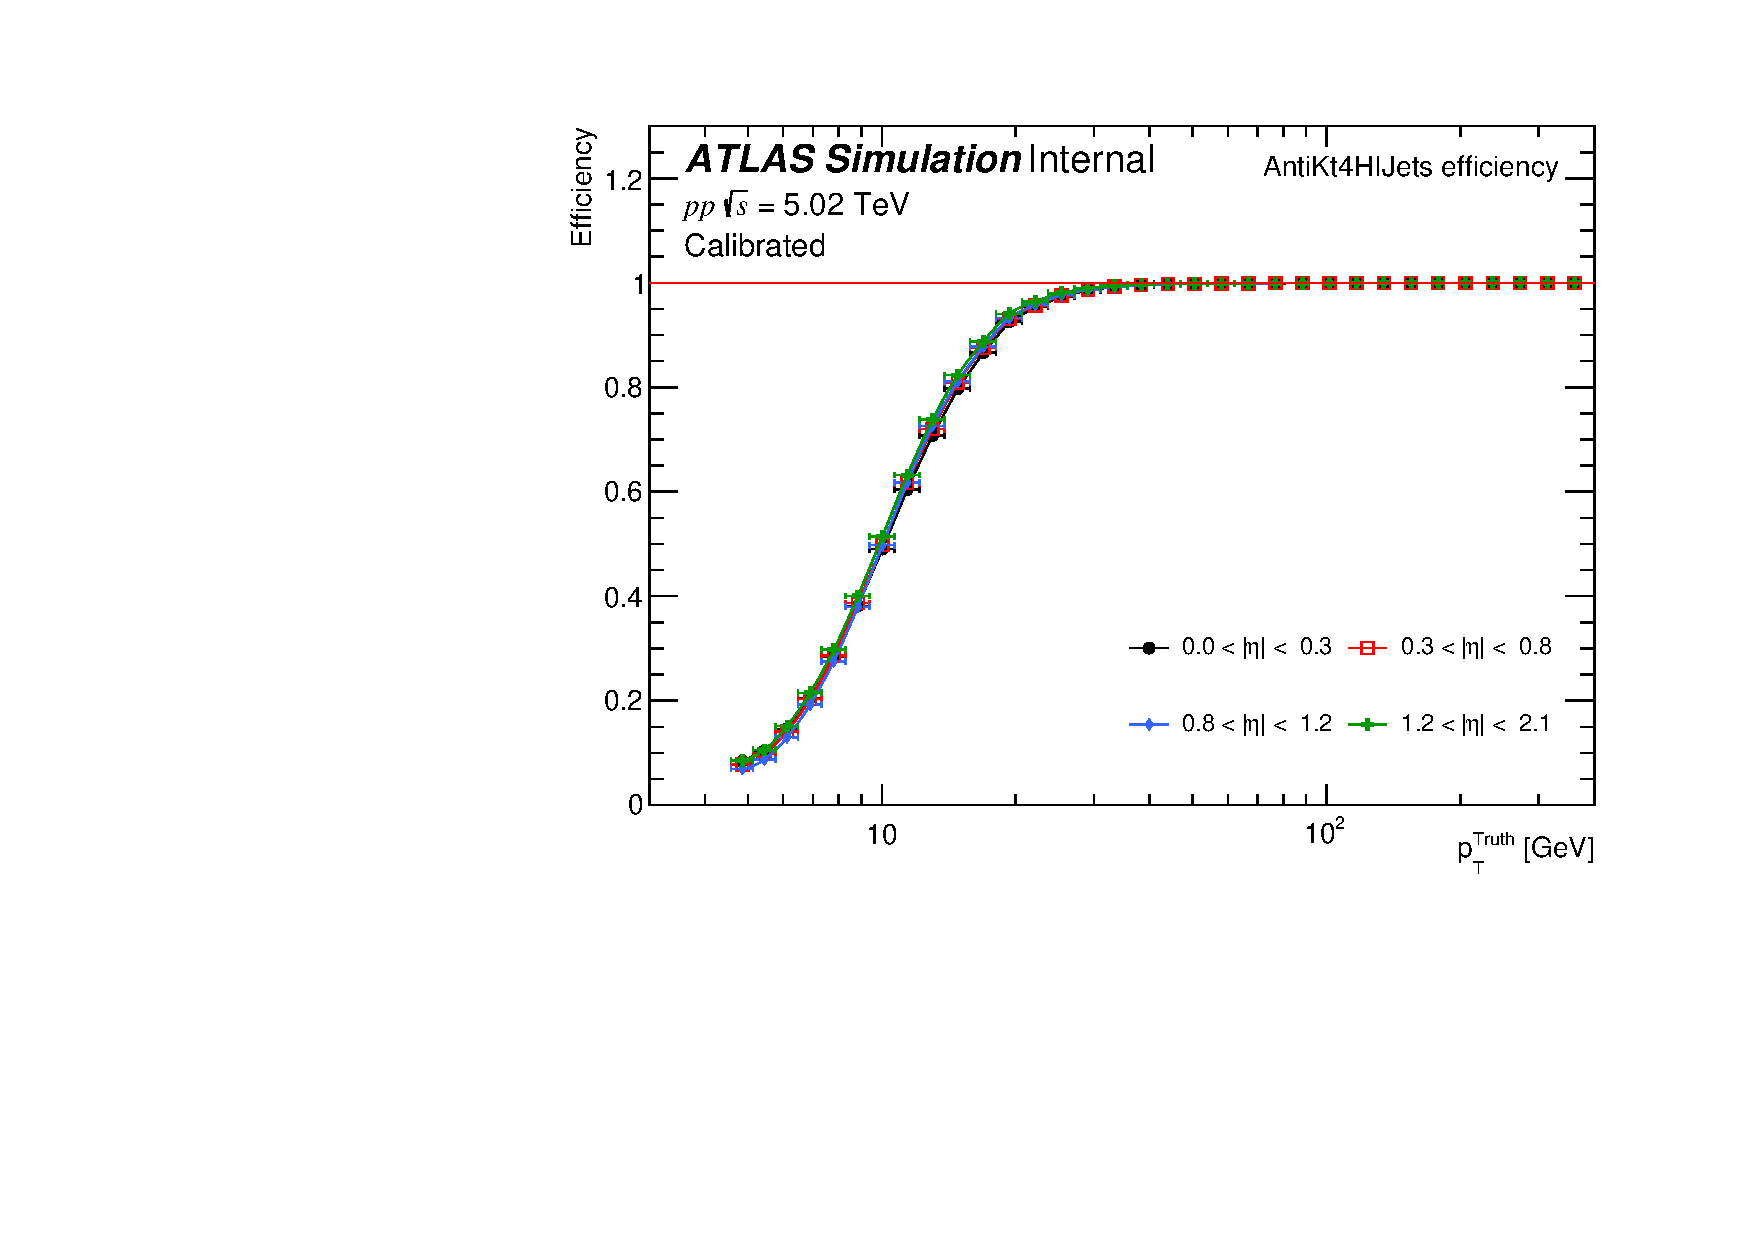
\includegraphics[width=7cm]{figures_general/Eff_pp5.pdf} &
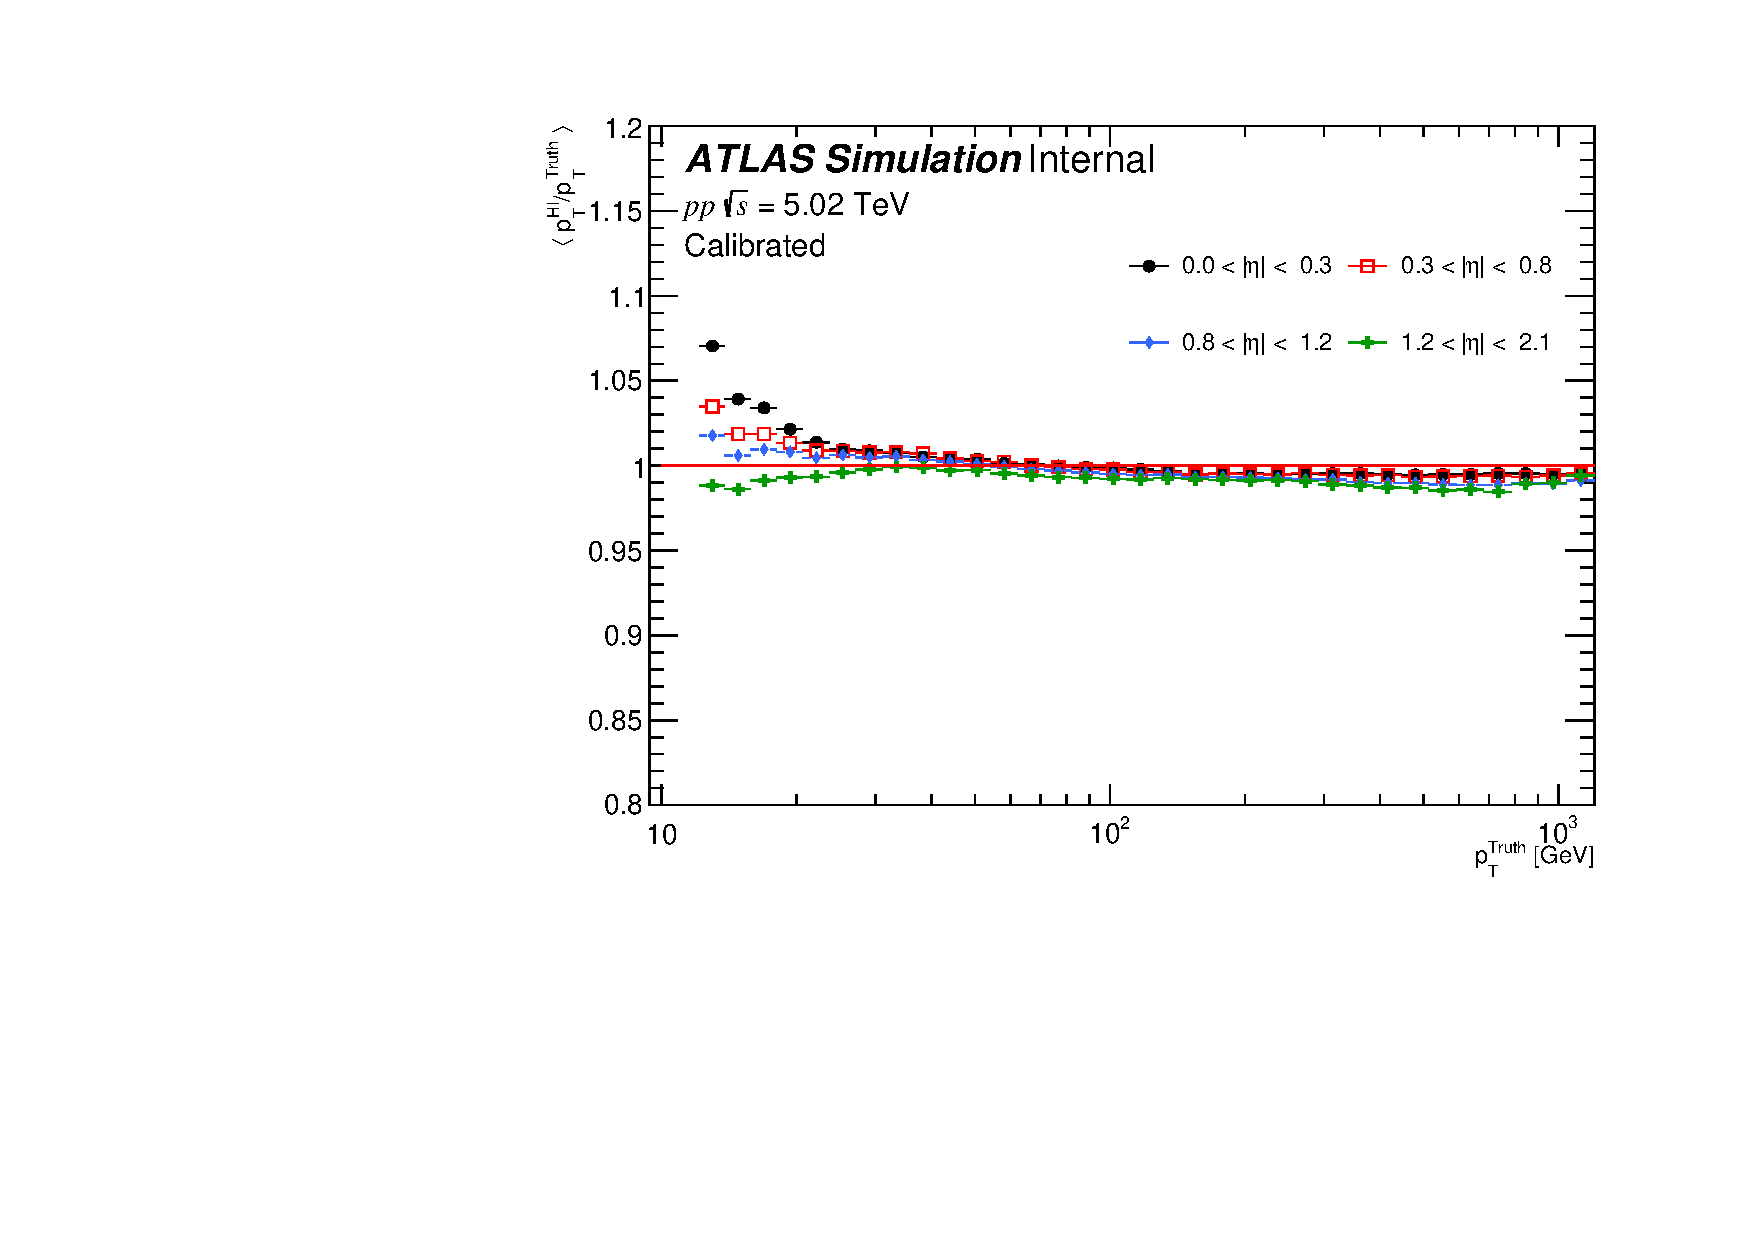
\includegraphics[width=7.3cm]{figures_general/JES_pp5.pdf} \\
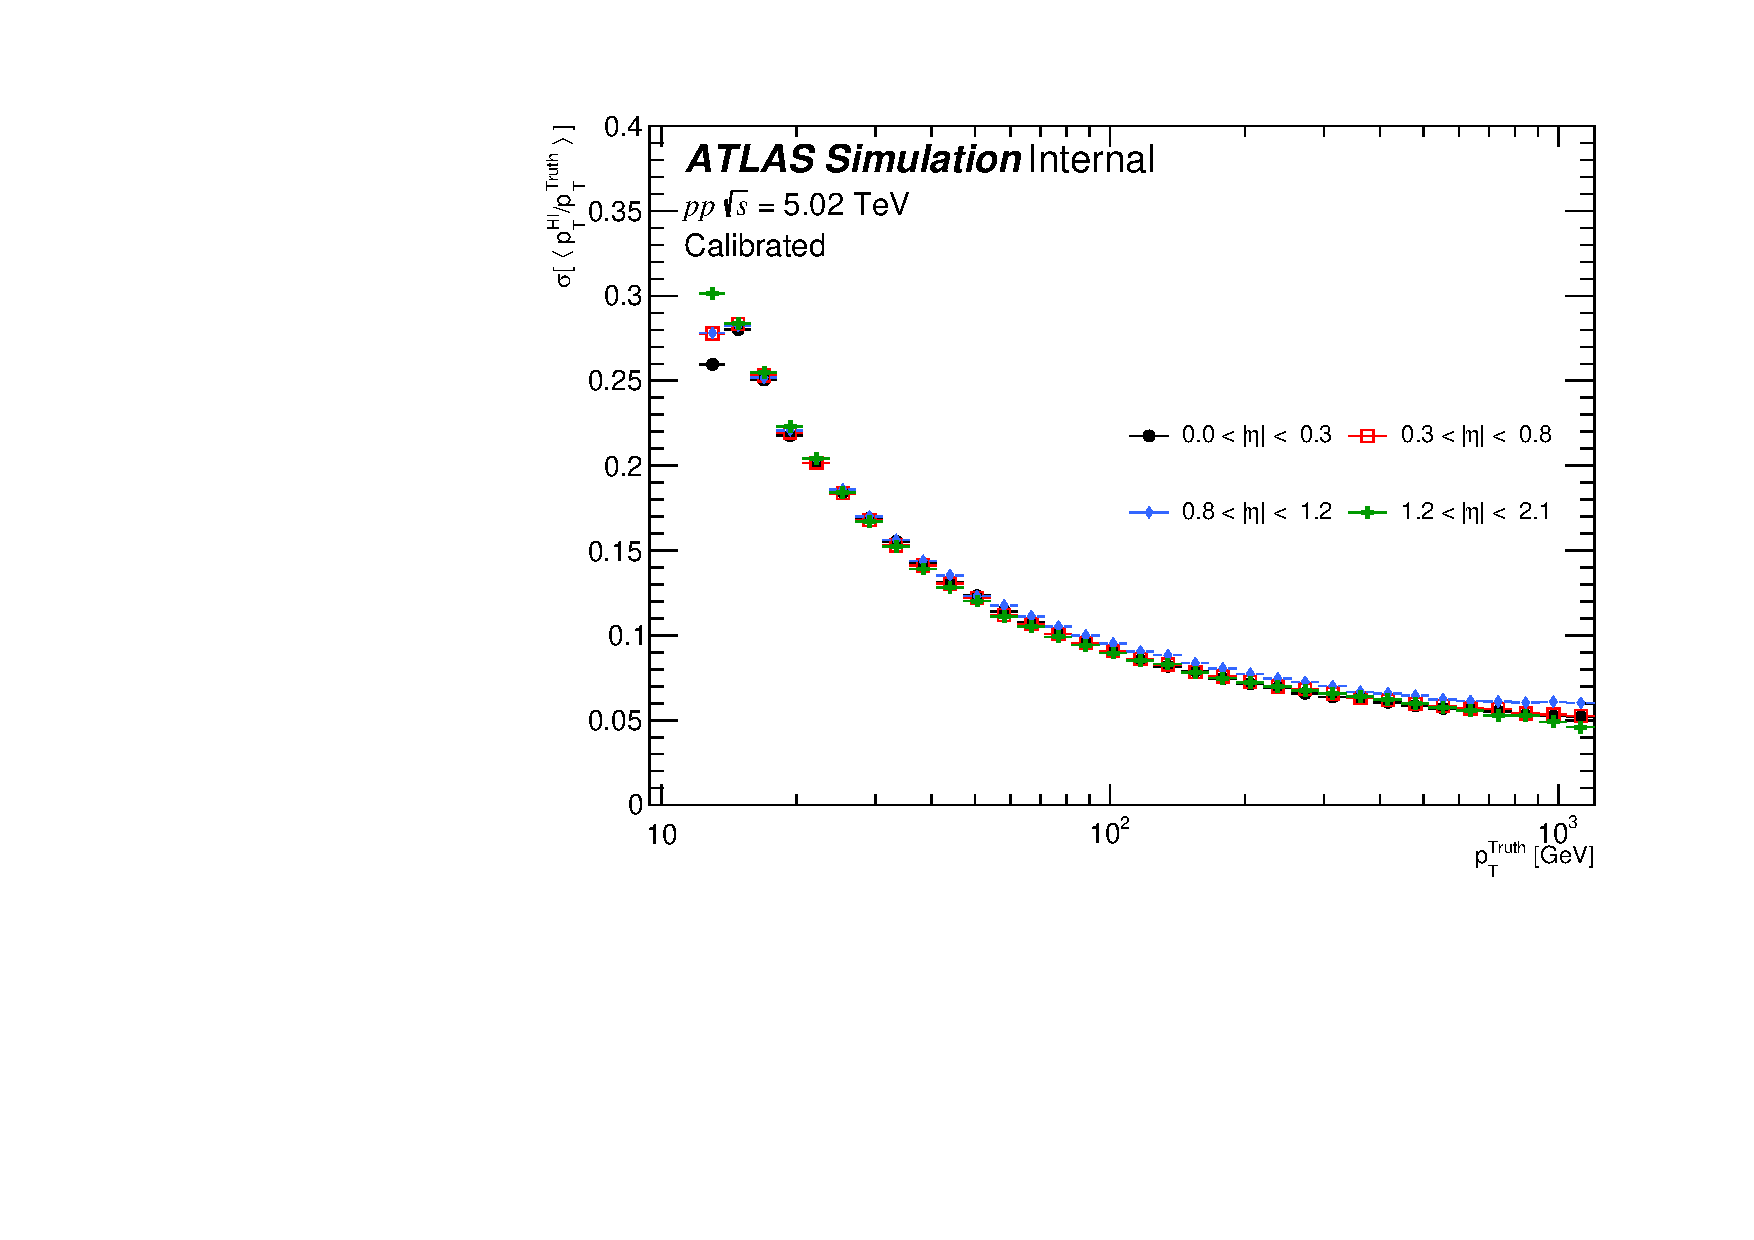
\includegraphics[width=7.3cm]{figures_general/JER_pp5.pdf} 
\end{tabular}}
\caption{
Top panels: Jet reconstruction efficiency in 5.02 TeV \pp\ collisions (left) as a function of truth jet \pT\ and different $\eta$ bins. Jet energy scale (JES) in 5.02 TeV \pp\ collisions (right) as a function of truth jet \pT\ and different $\eta$ bins. Bottom panels: Jet energy resolution (JER) in 5.02 \pp\ collisions as a function of truth jet \pT\ and different $\eta$ bins.
}
\label{Fig:Performancepp5}
\end{figure}

\begin{figure}
   \centering
   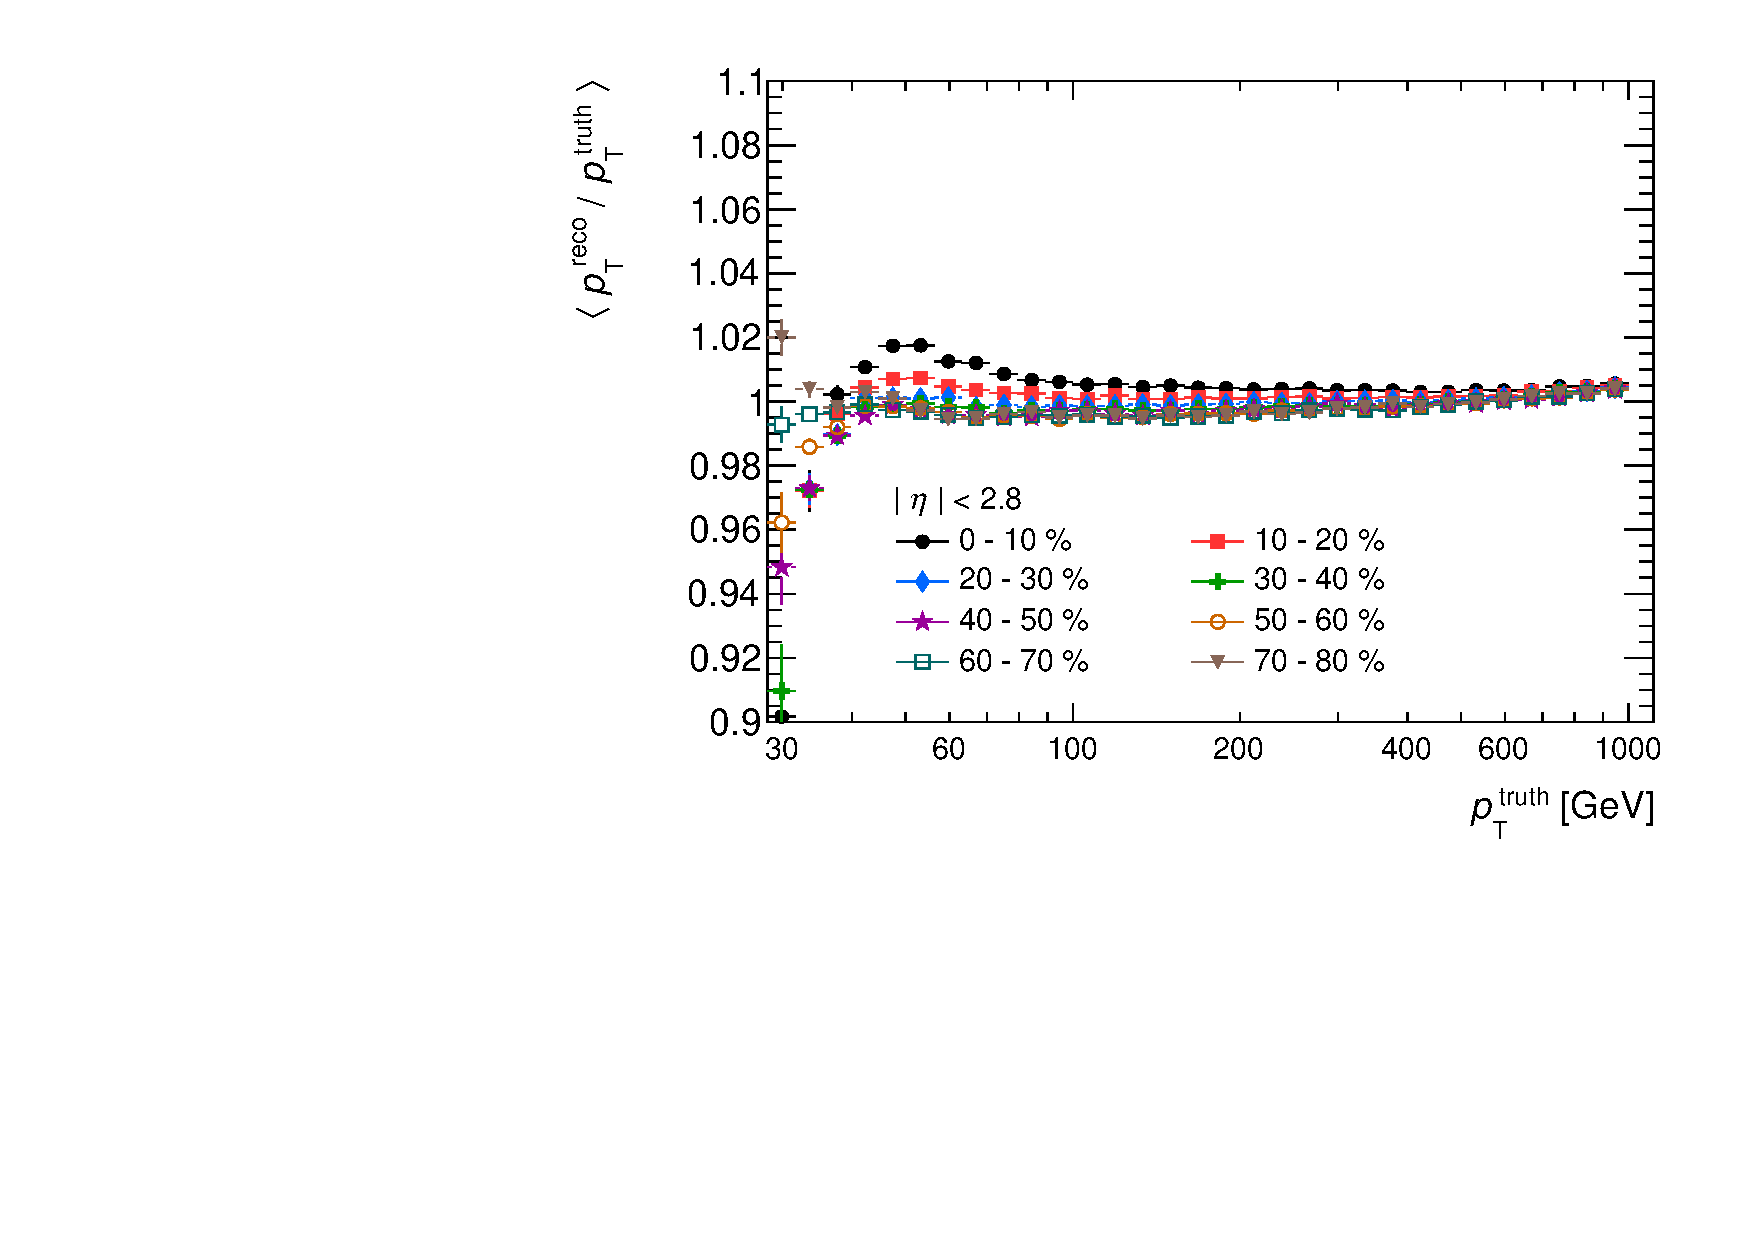
\includegraphics[width = 0.75\textwidth]{figures_general/PbPb_JES_pT_eta2p8.pdf}
   \caption{ JES in \pbpb\ collisions for eight centrality selections.  Plot is from Ref.~\cite{PbPbRaaNote}.}
   \label{Fig:PerformancepbpbJES}
\end{figure}

\begin{figure}
   \centering
   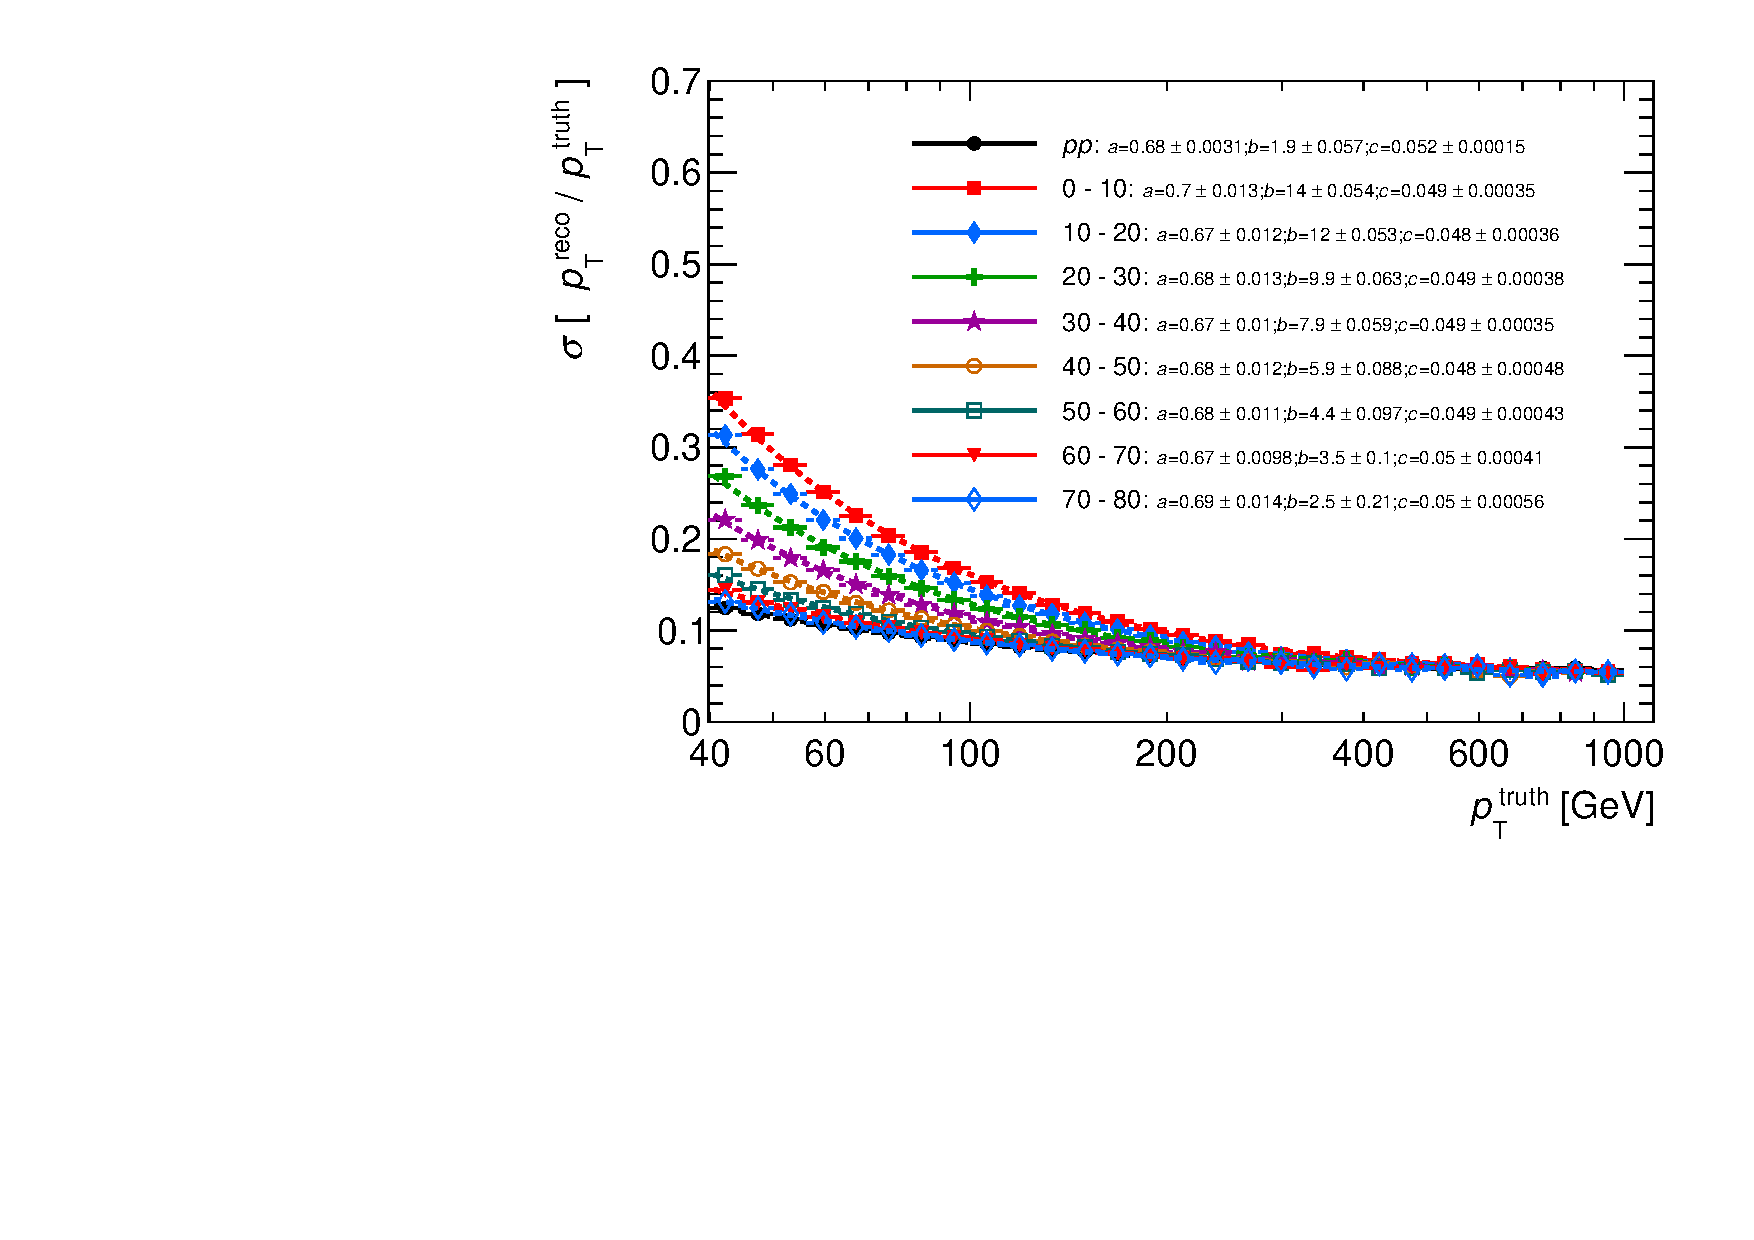
\includegraphics[width = 0.75\textwidth]{figures_general/PbPb_JER_pT_eta2p8.pdf}
   \caption{ JER in \pbpb\ collisions for eight centrality selections.  Plot is from Ref.~\cite{PbPbRaaNote}. The points are fit to the standard function that describes the calorimetric resolution.}
   \label{Fig:PerformancepbpbJER}
\end{figure}


\begin{figure}
   \centering
   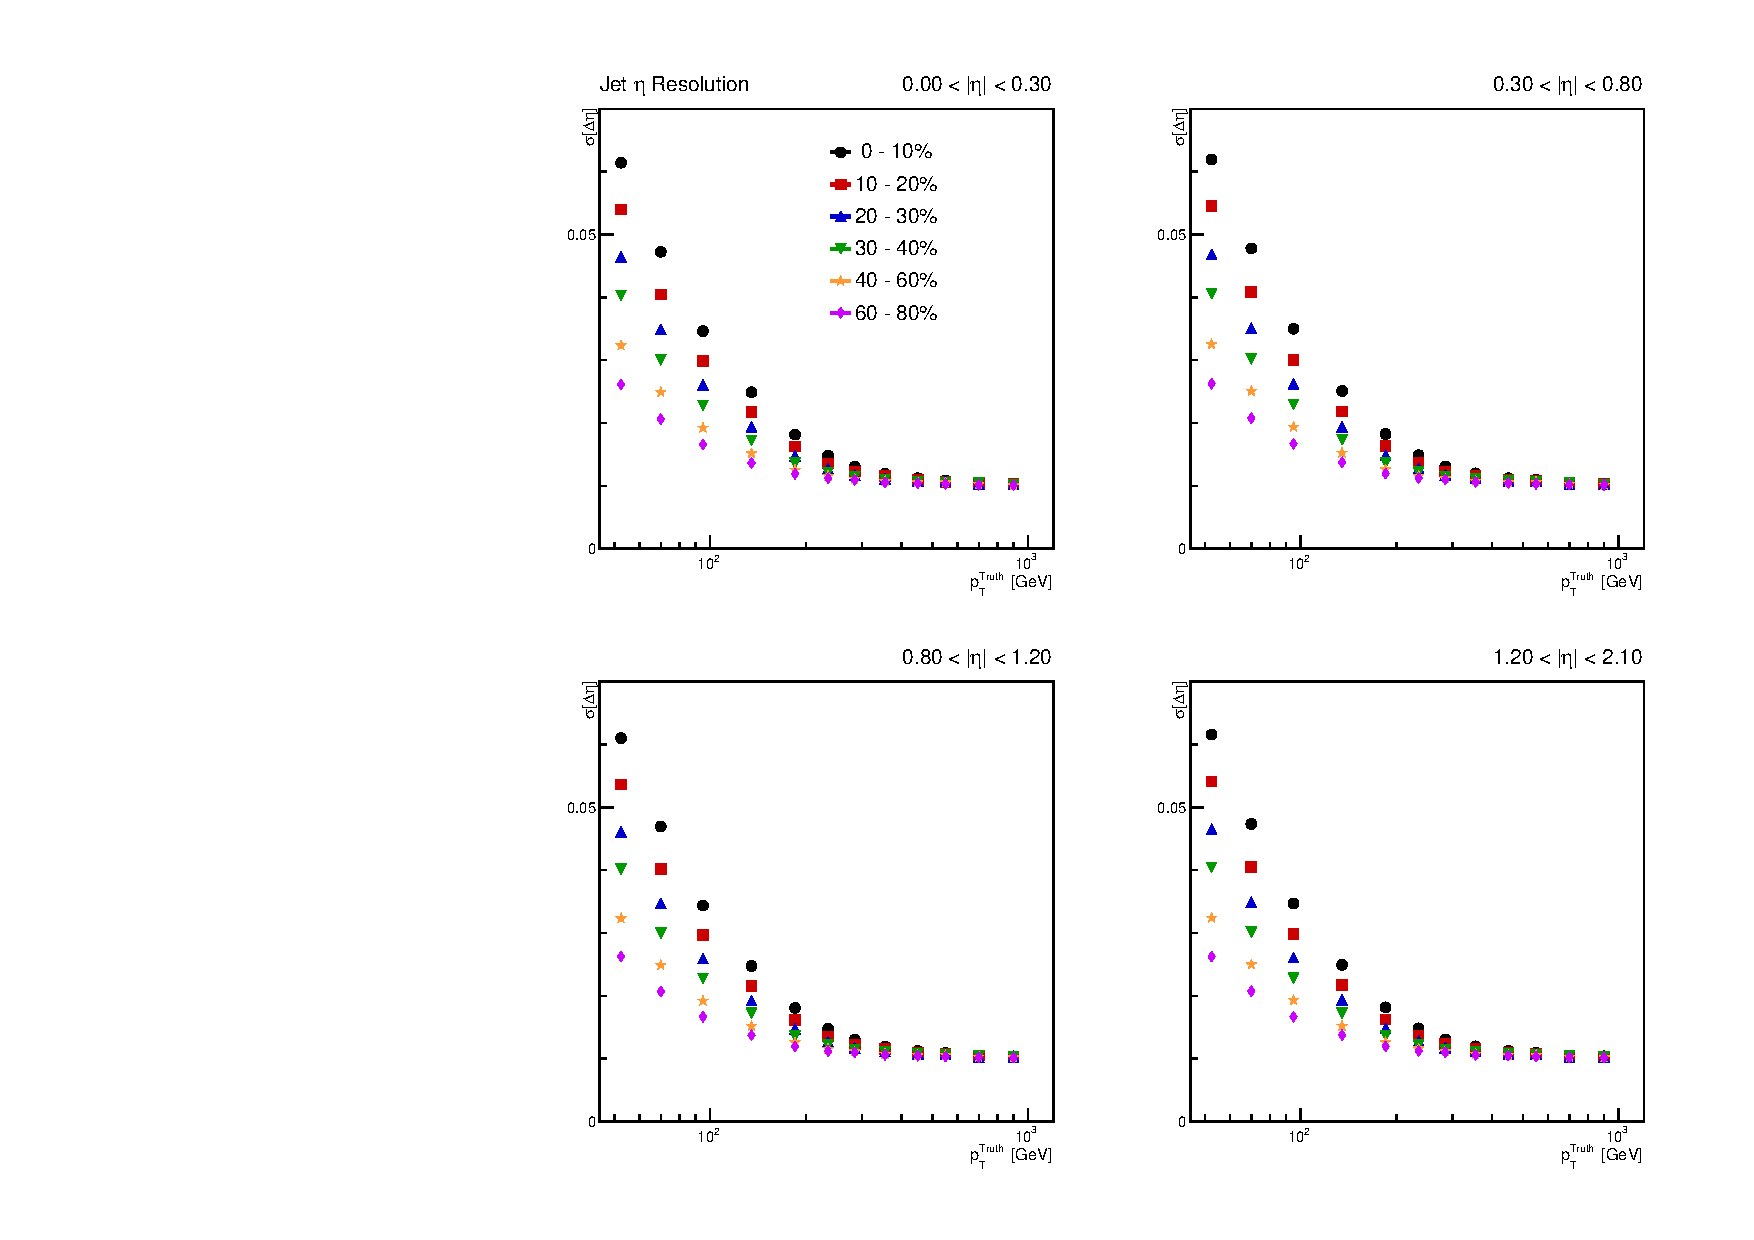
\includegraphics[width = 0.75\textwidth]{figures_general/jet_res_eta_r04.pdf}
   \caption{ Jet angular resolution in $\eta$ for $R=0.4$ jets in \pbpb\ collisions as a function of jet \pT\ for six centrality selections.}
   \label{Fig:PerformancepbpbJPReta0p4}
\end{figure}

\begin{figure}
   \centering
   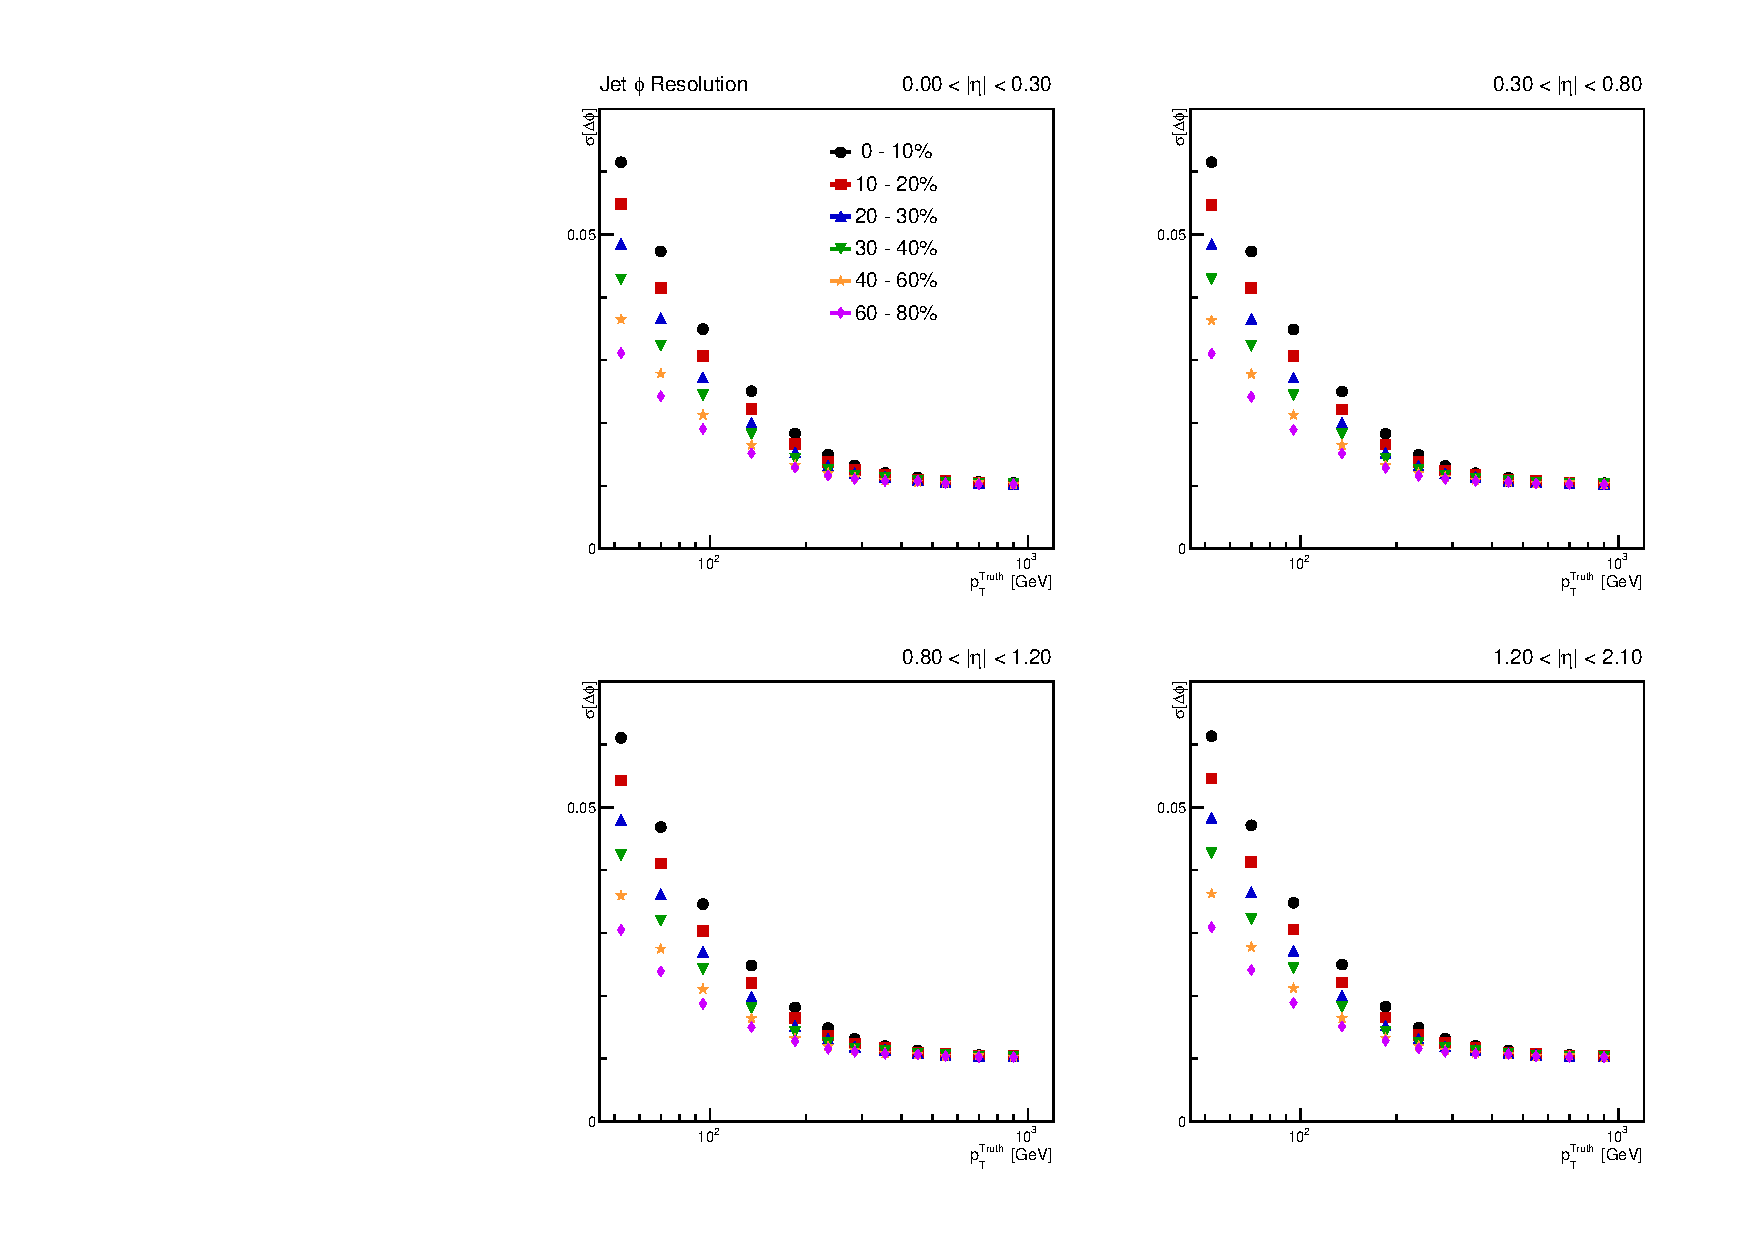
\includegraphics[width = 0.75\textwidth]{figures_general/jet_res_phi_r04.pdf}
   \caption{ Jet angular resolution in $\phi$ for $R=0.4$ jets in \pbpb\ collisions as a function of jet \pT\ for six centrality selections.}
   \label{Fig:PerformancepbpbJPRphi0p4}
\end{figure}

%\begin{figure}
%   \centering
%   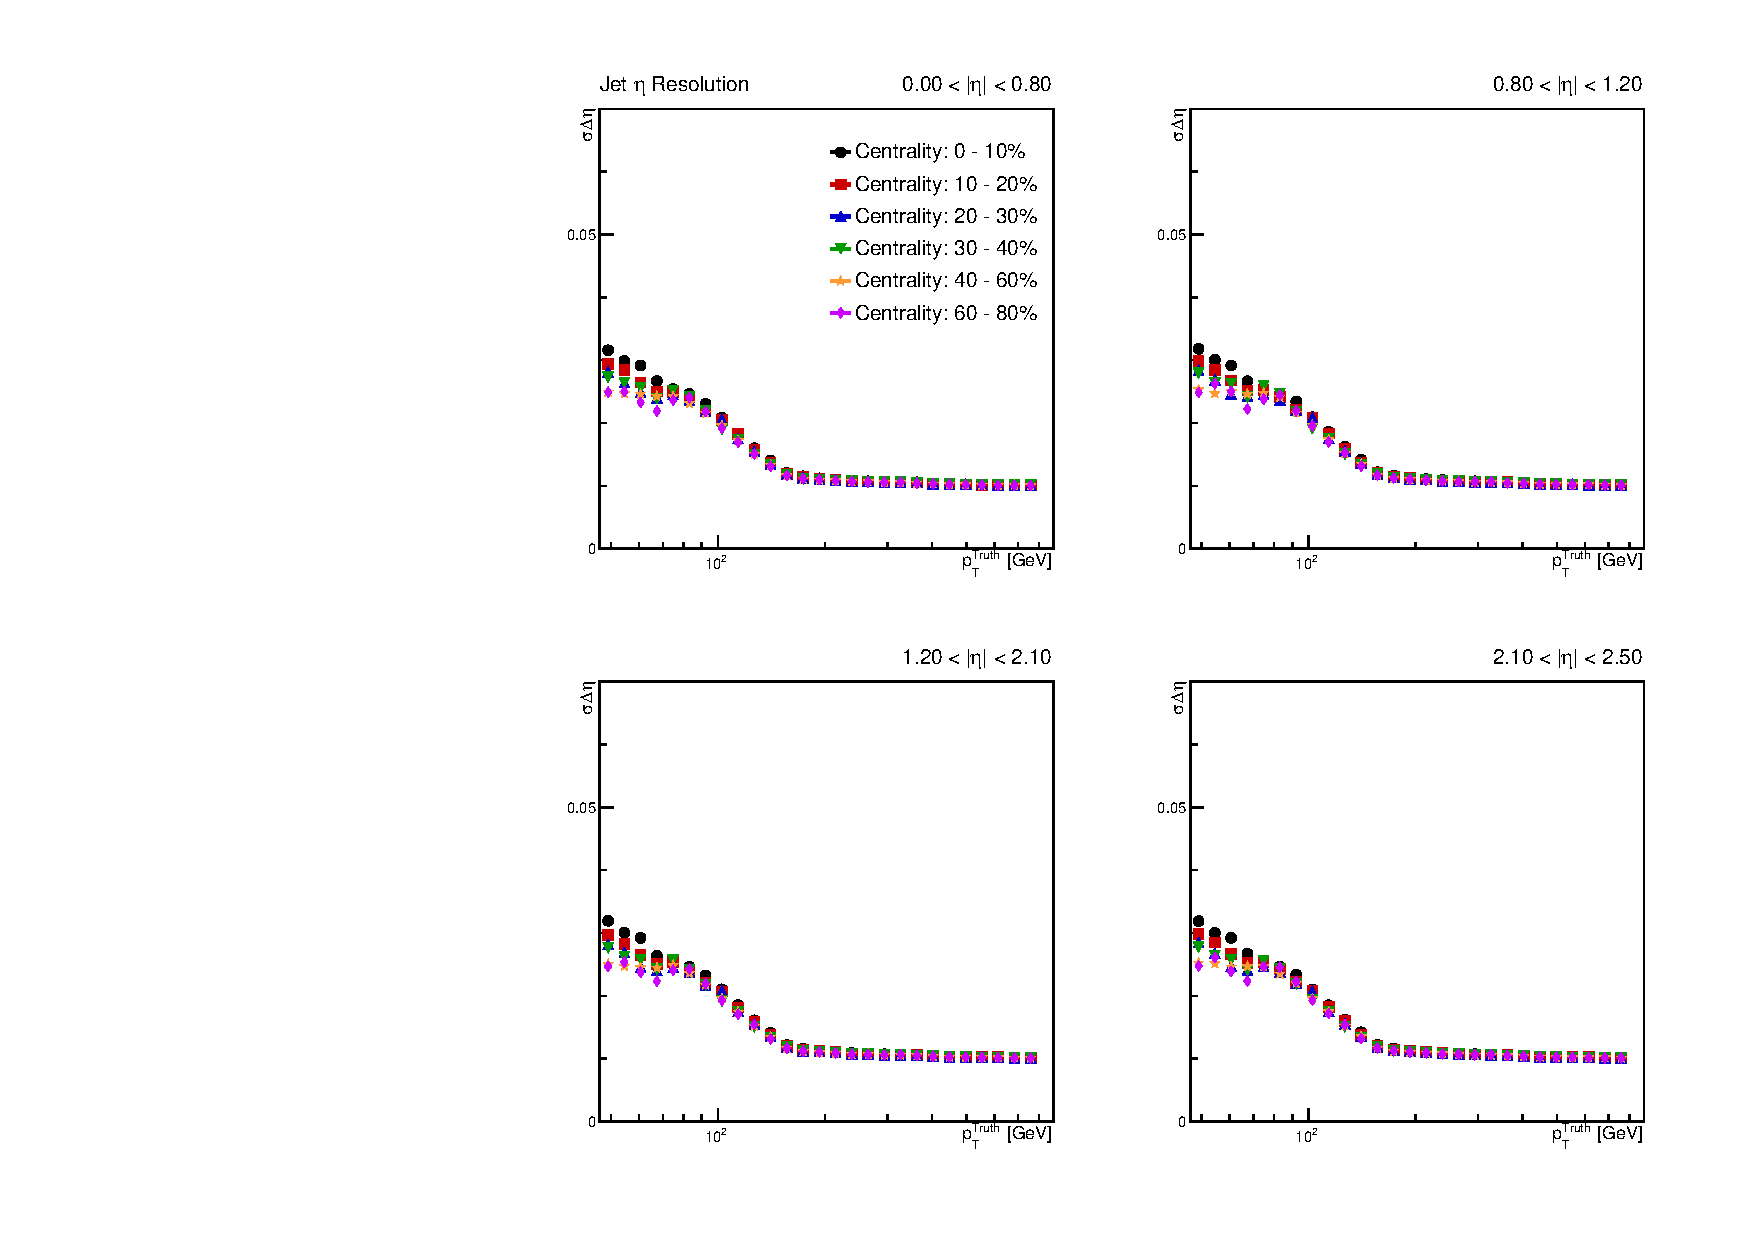
\includegraphics[width = 0.75\textwidth]{figures_general/jet_res_eta_r02_new.pdf}
%   \caption{ Jet angular resolution in $\eta$ for $R=0.2$ jets in \pbpb\ collisions as a function of jet \pT\ for six centrality selections.}
%   \label{Fig:PerformancepbpbJPReta0p2}
%\end{figure}
%
%\begin{figure}
%   \centering
%   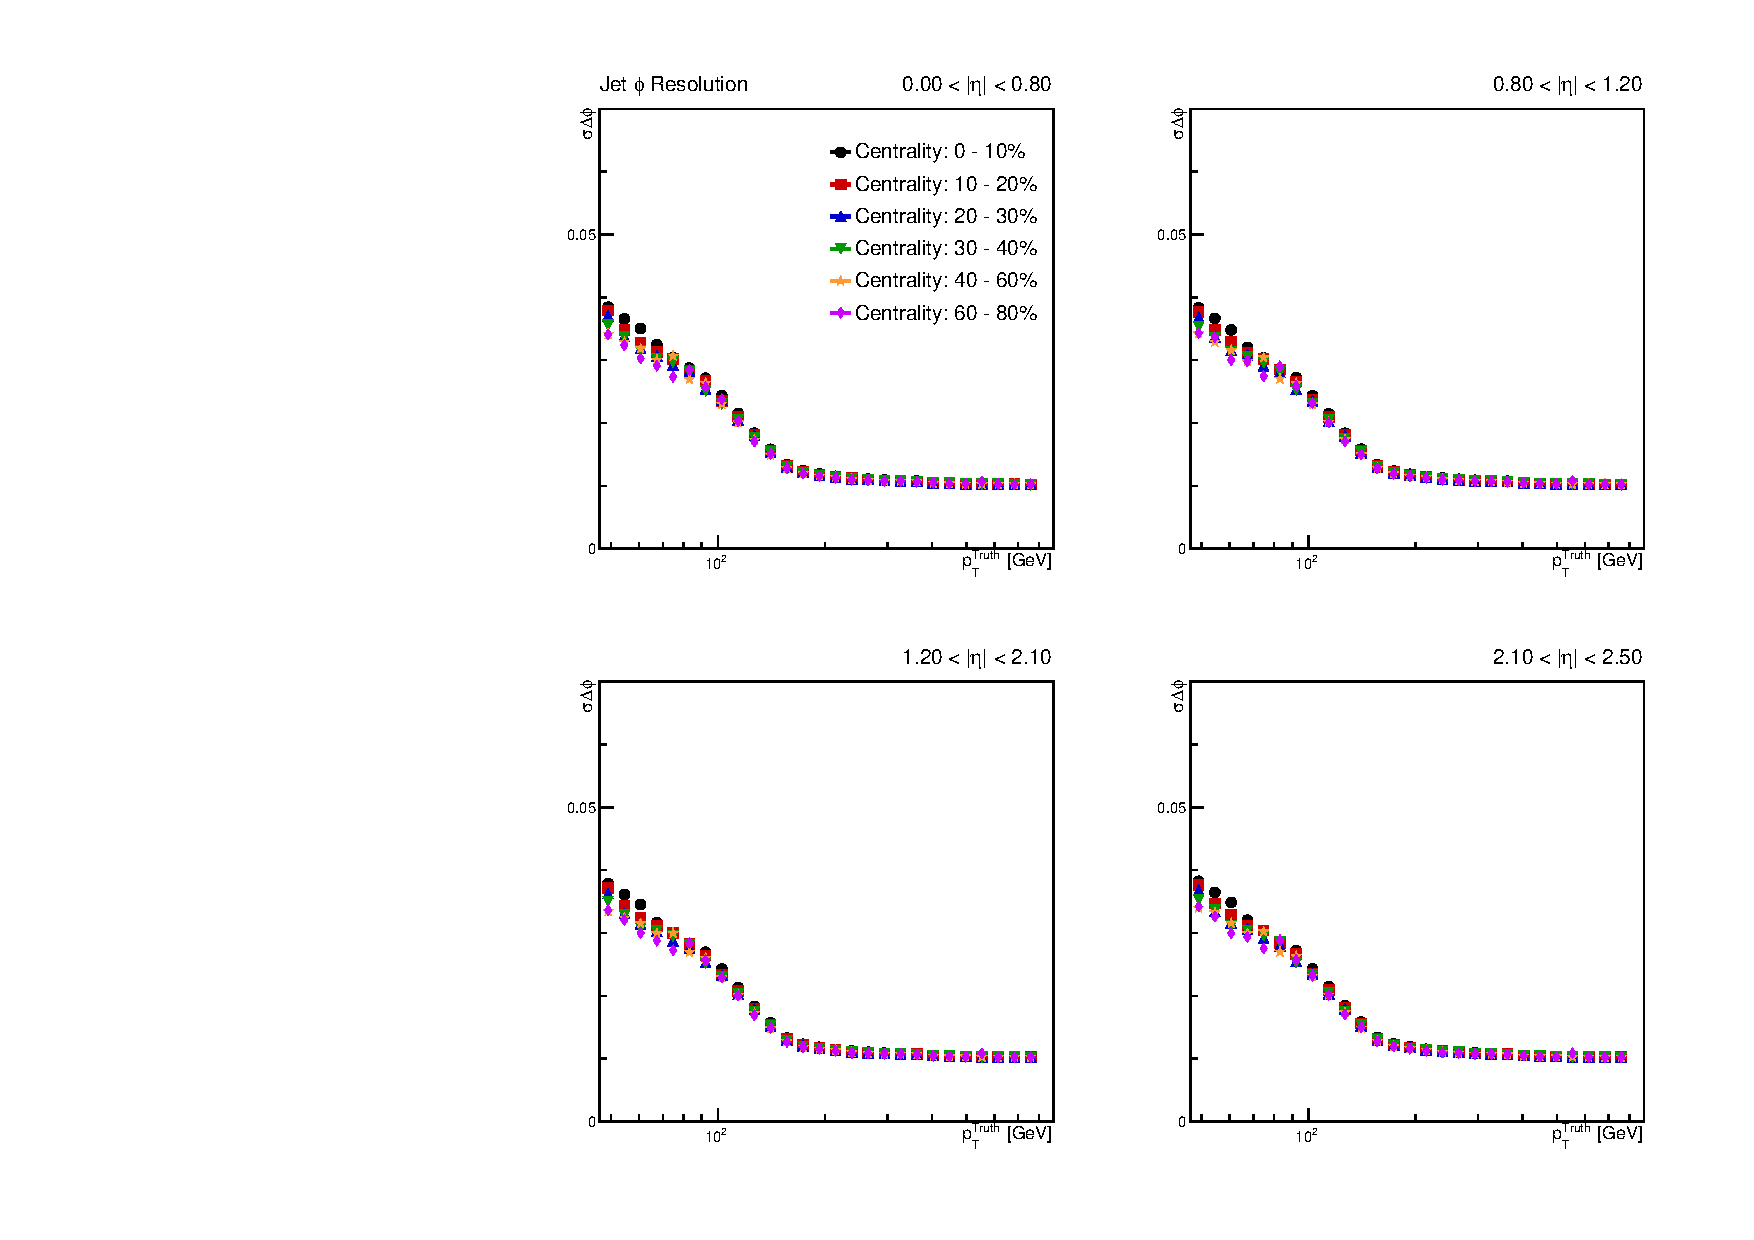
\includegraphics[width = 0.75\textwidth]{figures_general/jet_res_phi_r02_new.pdf}
%   \caption{ Jet angular resolution in $\phi$ for $R=0.2$ jets in \pbpb\ collisions as a function of jet \pT\ for six centrality selections.}
%   \label{Fig:PerformancepbpbJPRphi0p2}
%\end{figure}

\clearpage
%%%%%%%%%%%%%%%%%%%%%%%%%%%
\section{Basic Cuts and Corrections}
\label{sec:cuts_corrections}
% !TEX root = trackjet_intnote.tex

A description of the analysis procedure to reconstruct the $\Dptr$ distribution, along with the derivation and application of the various corrections is presented in the following sections. The analysis structure is illustrated by the diagram in Fig.~\ref{Fig:analysis_flow} where each part of the analyses is described in a separate subsection and it can be summarized as follows: 


\begin{itemize}
\item Jet selection and calibration
\item Track selection
\item Track momentum correction
\item Fake rates
\item Tracking efficiency
\item Underlying event subtraction of tracks
\item Unfolding
\end{itemize}


\subsection{Jet Selection and final energy calibration}
\label{Sec:JetSelection}
Since the Inner Detector (ID) covers the $|\eta| < 2.5$, the analysis can 
only be performed for jets within the pseudorapidity interval of $|\eta| < 1.7$ to have the entire $r=$0.8 cone under investigation fully covered by the tracking detector. In both collision systems, jets are 
measured with \ptjet\ between 126~GeV and 316~GeV in following four successive intervals: 126--158, 158--200, 200--251, and 251--316~GeV. This binning was motivated by the large fake rate below 100 \GeV. An underflow bin was also needed for the unfolding procedure, and hence, the measurement starts at 126 \GeV. This binning is also used in previous heavy ion jet measurements (\cite{ATLAS502FFConf}). Truth jets were associated with the nearest reconstructed jet using the matching of $\dR<0.2$ for the performance study and to build response matrices for the unfolding procedure. The same \dR\ matching criteria were employed in previous ATLAS HI jet analyses and are justified by a detailed performance study~\cite{Aad:12081967v1}. To prevent nearby jets from distorting the measurement of \Dptr\ distributions, 
jets are rejected if there is another jet with a higher \ptjet\ than the considered jet anywhere
within a distance of $\Delta R < 1.0$. The isolation cut removes approximately 0.01\% of jets (see Figure \ref{fig:ISO}), and has almost no impact on the final measurement.

\begin{figure}
\centering{
\begin{tabular}{cc}
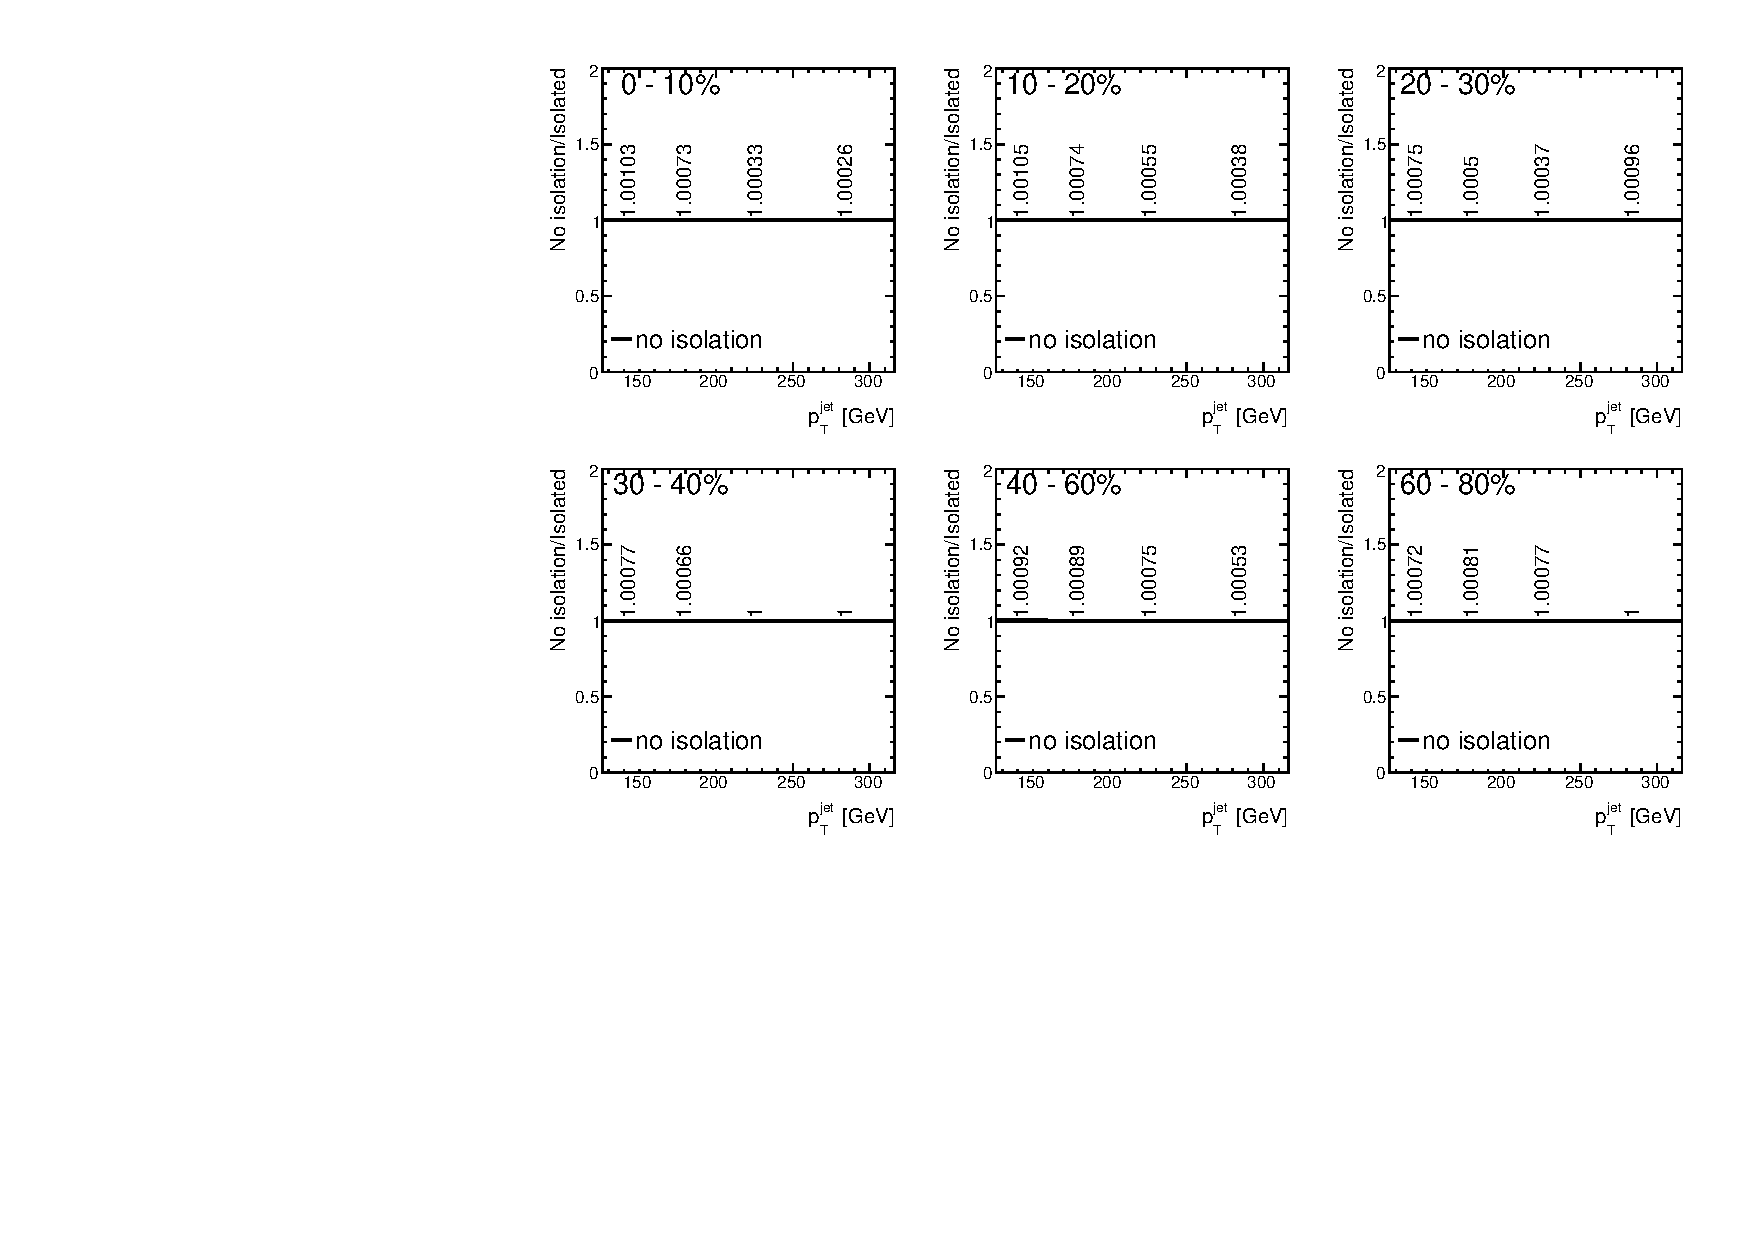
\includegraphics[width=0.9\textwidth]{figures_performance/jet_iso.pdf} \\
\end{tabular}}
\caption{The ratios of the jet spectra with no isolation to that with isolation in the kinematic range of interest for \pbpb\ collisions, in all centralities. The isolation requirement rejects less that 0.1\% of jets, and has almost no impact on the final measurement}
\label{fig:ISO}
\end{figure}  




A final calibration, referred to as a cross-calibration��~\cite{cc2015}, 
was applied to the data to account for observed differences in the calorimetric response between data and MC. The cross-calibration factors were estimated using in-situ calibration studies~\cite{HIjesnote} where jets are measured in events while recoiling against objects for which the energy scale is well known. 
No correction for the jet reconstruction efficiency is necessary, as the analysis is performed in the jet \pT\ region where the jet reconstruction is fully efficient~\cite{ATLAS-COM-PHYS-2013-1369}. 

The jet energy measured in the calorimeter can be affected by the presence 
of dead cells or cells with a bad response, by noise spikes in the hadronic end-cap, by a noise in EM calorimeter and by out-of-time energy deposits from cosmic rays and beam backgrounds. In the \pp\ analysis, the set of recommended cuts of ``LooseBad'' is used to remove bad jets. The rate of these jets in the kinematic region of interest (100--316 \GeV) is less than 0.5\%. This cleaning procedure is not applied in \PbPb\ collisions because it is incompatible with the heavy ion jet reconstruction procedue, and also because the low luminosity ensures noise bursts are negligible. This is standard procedure for all heavy ion jet analyses.
 

%\subsection{Jet isolation}
%
%Jets were required to be isolated. Any jet having another jet with higher 
%\pt\ than the original jet within $\Delta R < 1.0$ has been discarded. Jet isolation has been required in 
%order to not bias the fragmentation measurement by a potential presence of 
%split jets. The procedure is adopted from the fragmentation analyses in \pp~\cite{Aad:2011sc,FF7TeVInt}. 
%
%To test the sensitivity of this requirement, the \pT\ threshold on the second jet within $\Delta R < 1.0$ was decreased to 80\% of the original jet. The ratios of the raw fragmentation functions with the default cut to version with the more strict isolation requirement applied is shown in Fig~\ref{fig:ISO80}. The impact of this correction is small and the difference in the measured distributions is less than 1\%.

%\begin{figure}
%\centering{
%\begin{tabular}{cc}
%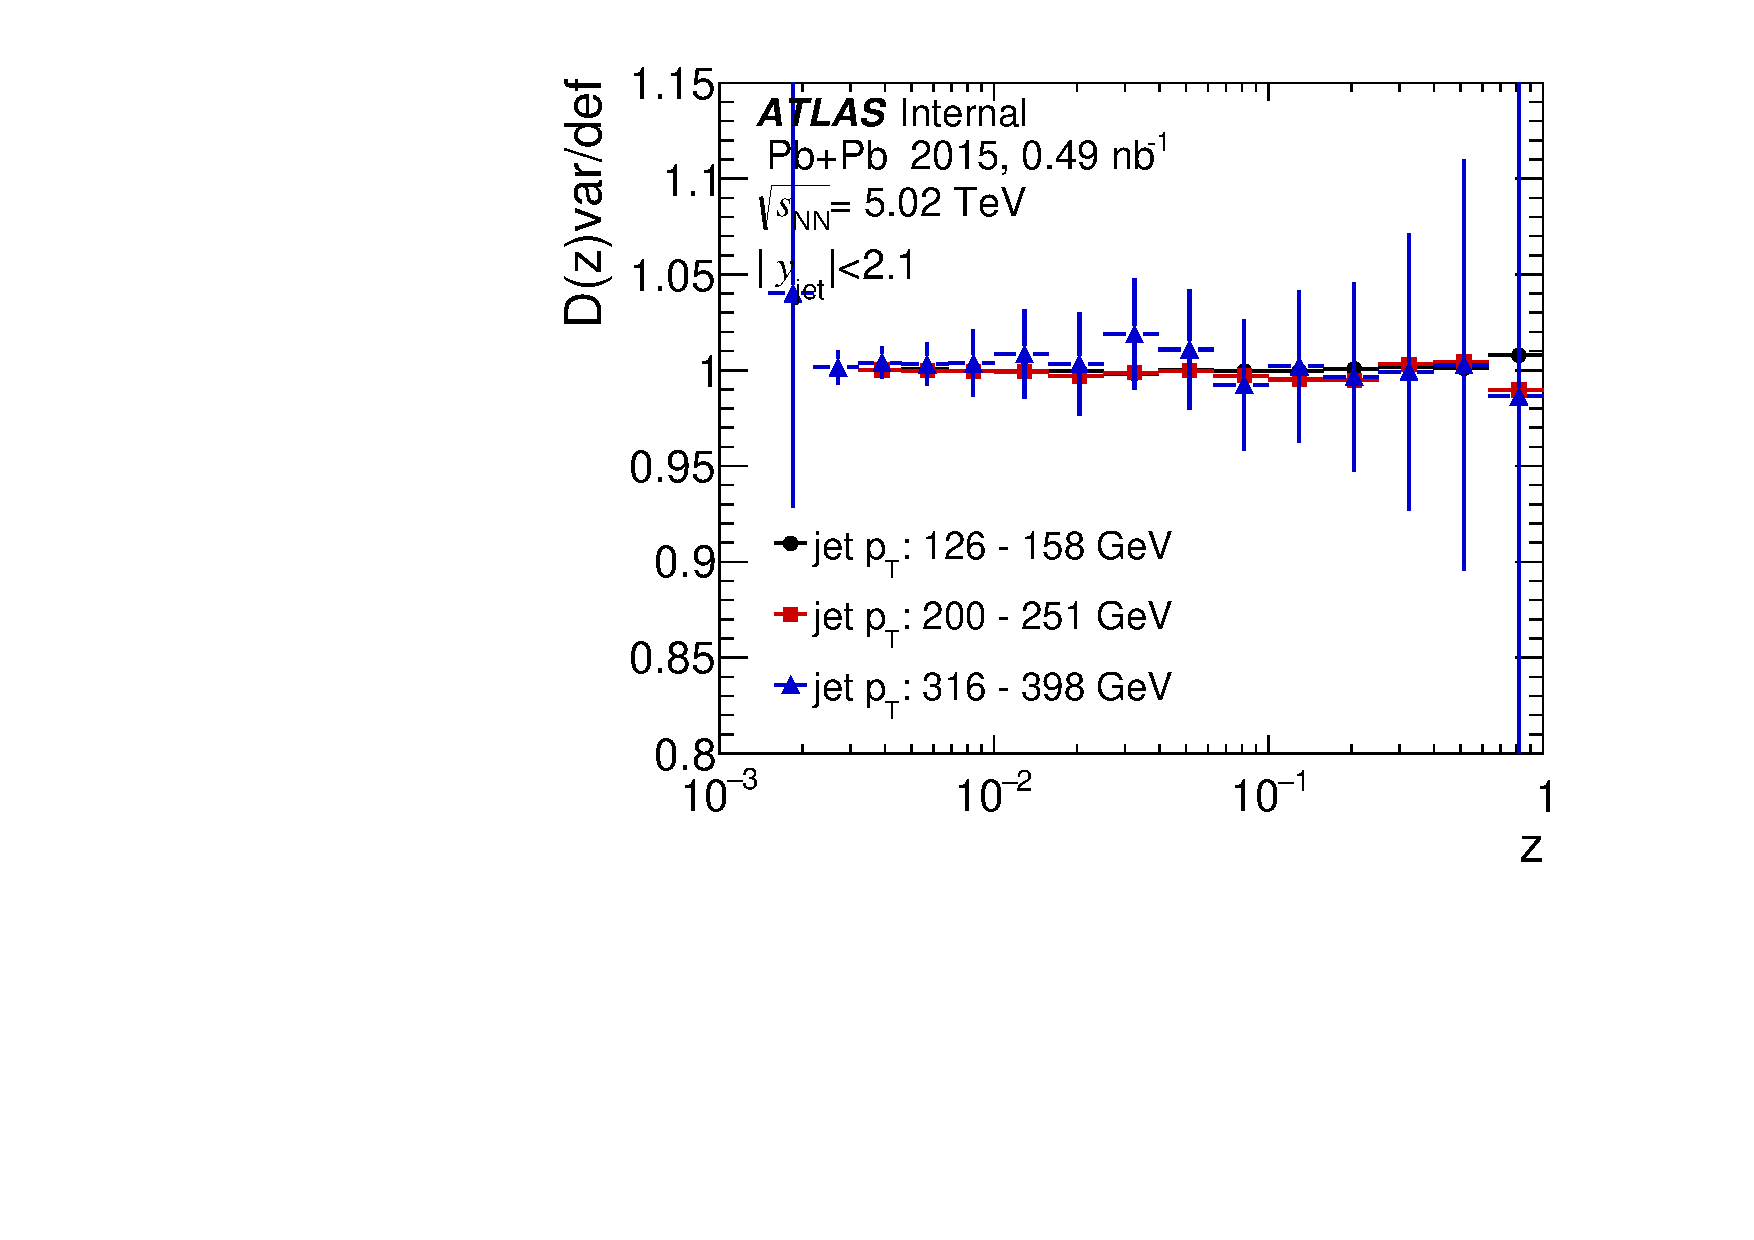
\includegraphics[width=0.45\textwidth]{figures_corrections/ff_data_comaparison_eta4_cent0_iso08.pdf} &
%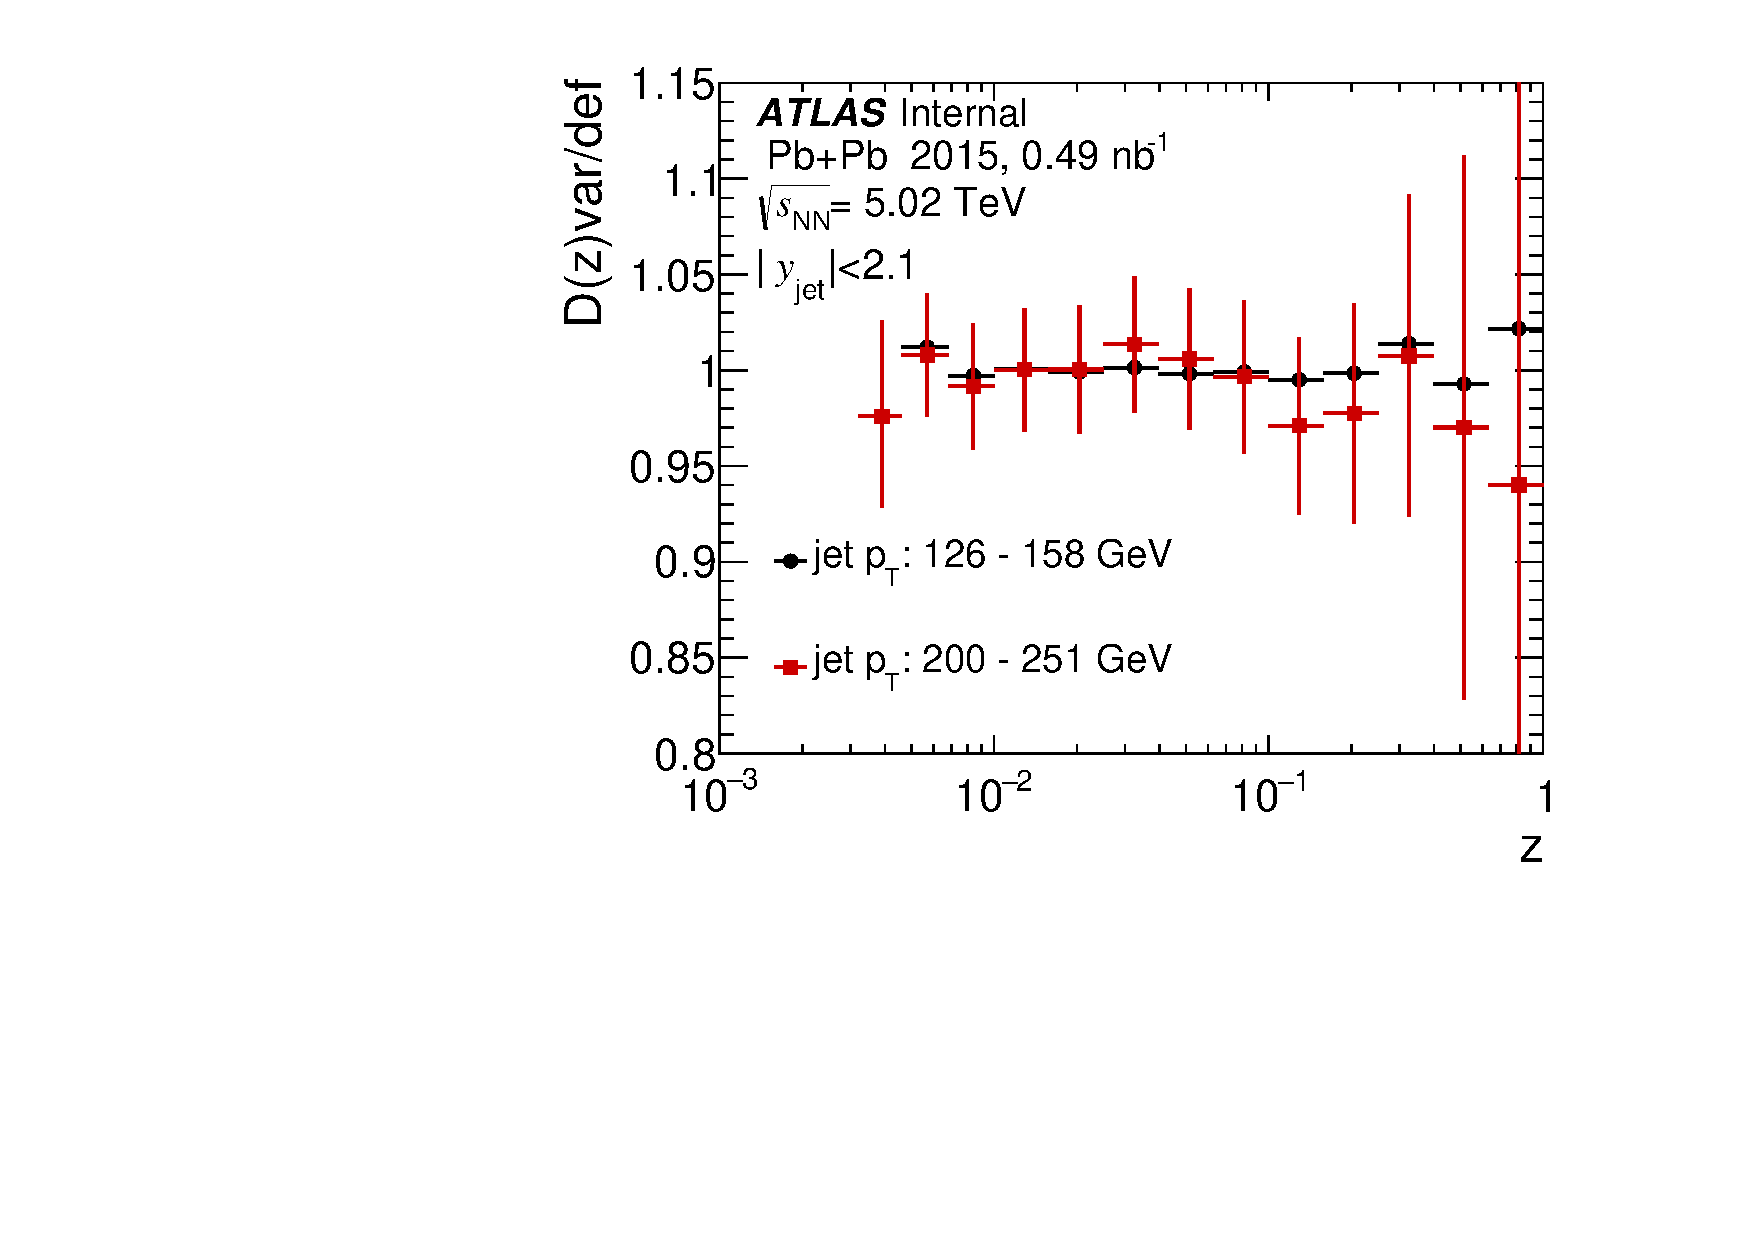
\includegraphics[width=0.45\textwidth]{figures_corrections/ff_data_comaparison_eta4_cent5_iso08.pdf} \\
%\end{tabular}}
%\caption{The ratios of the raw fragmentation functions evaluated with the more strict isolation requirement to the default version in \PbPb\ data in central (left) %and peripheral (right) collisions.}
%\label{fig:ISO80}
%\end{figure}  

%Fig.~\ref{fig:RdR} presents conditional yield of jets with $\pt^{2}$ that accompany a higher \pt\ jet with $\pt^{1}$ as a function of their angular separation $\mathrm{d}R$ in different centrality classes.
%\begin{figure}
%\centering{
%\begin{tabular}{cc}
%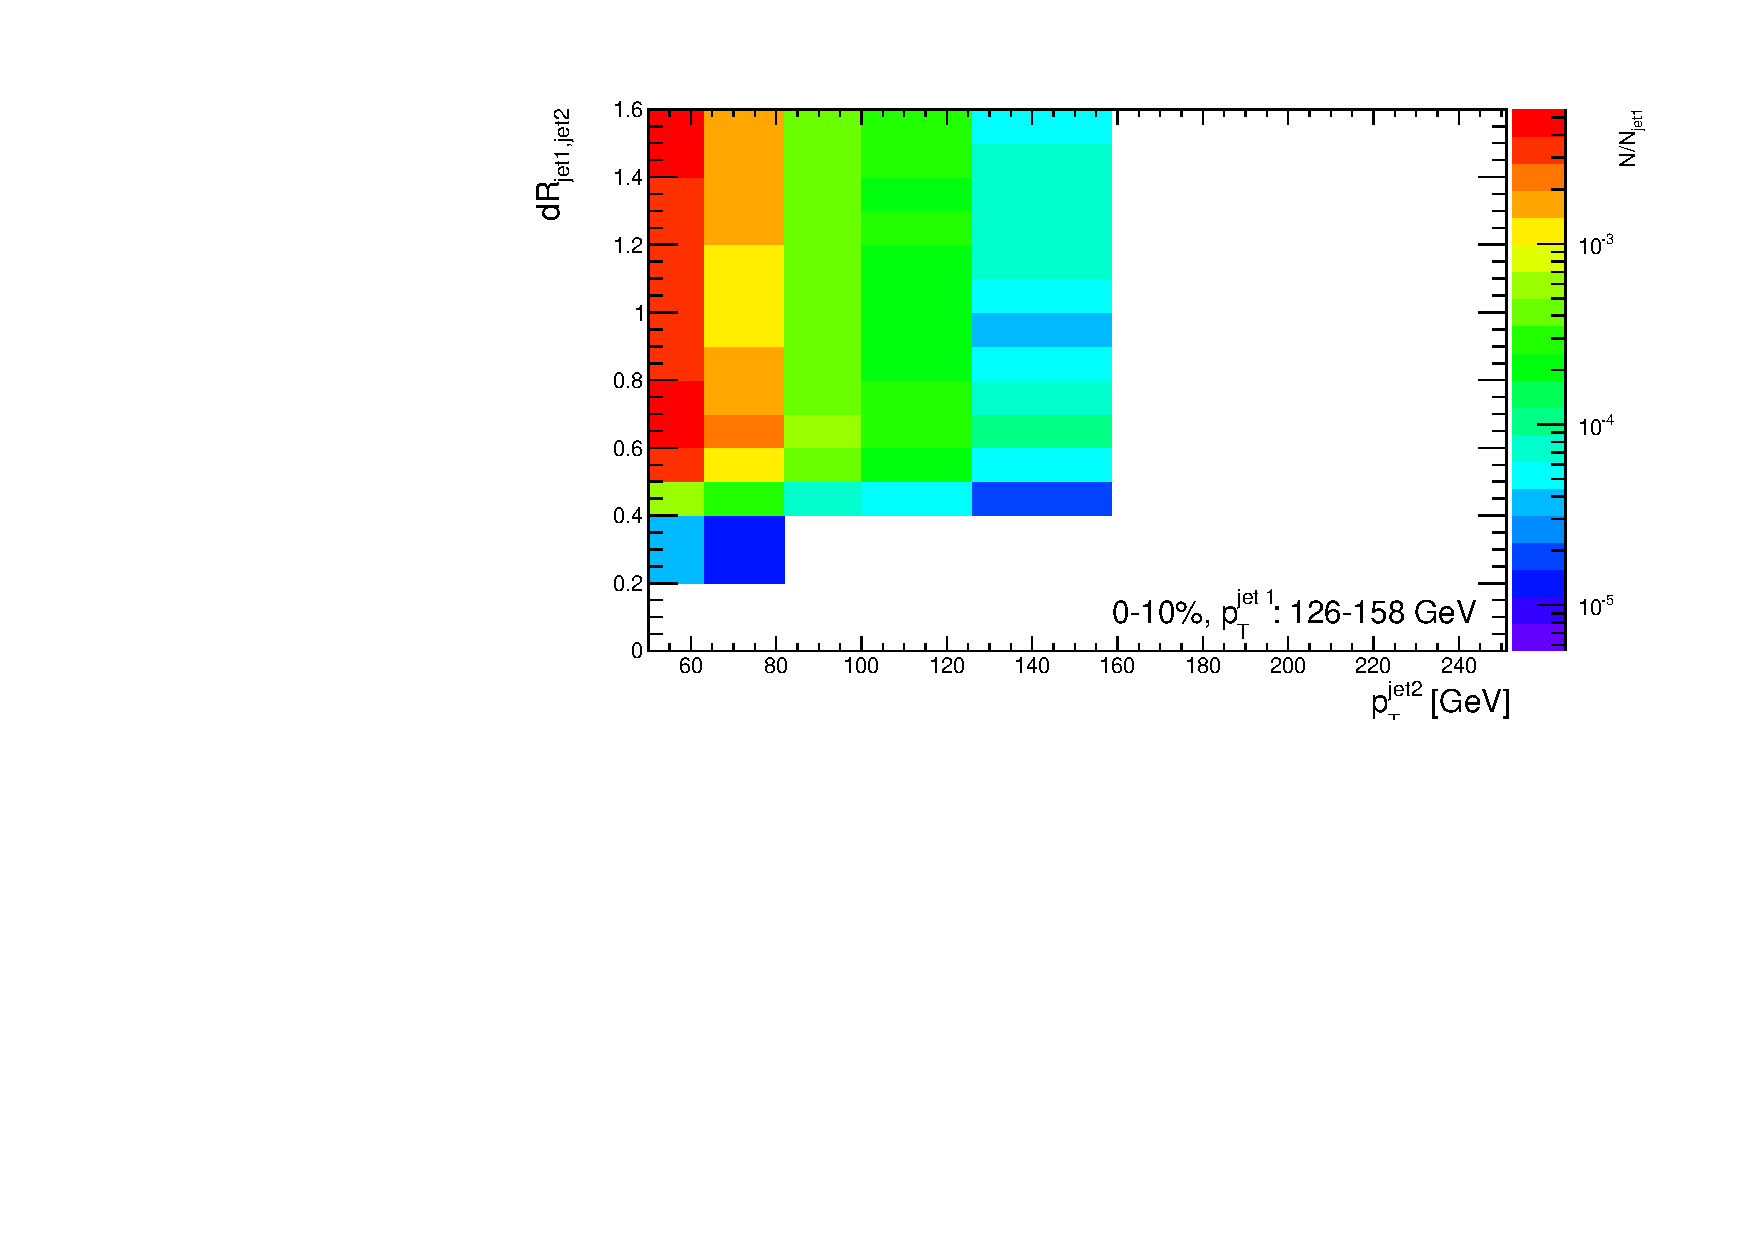
\includegraphics[width=0.45\textwidth]{figures_corrections/RdR_126_158GeV_c0.pdf} &
%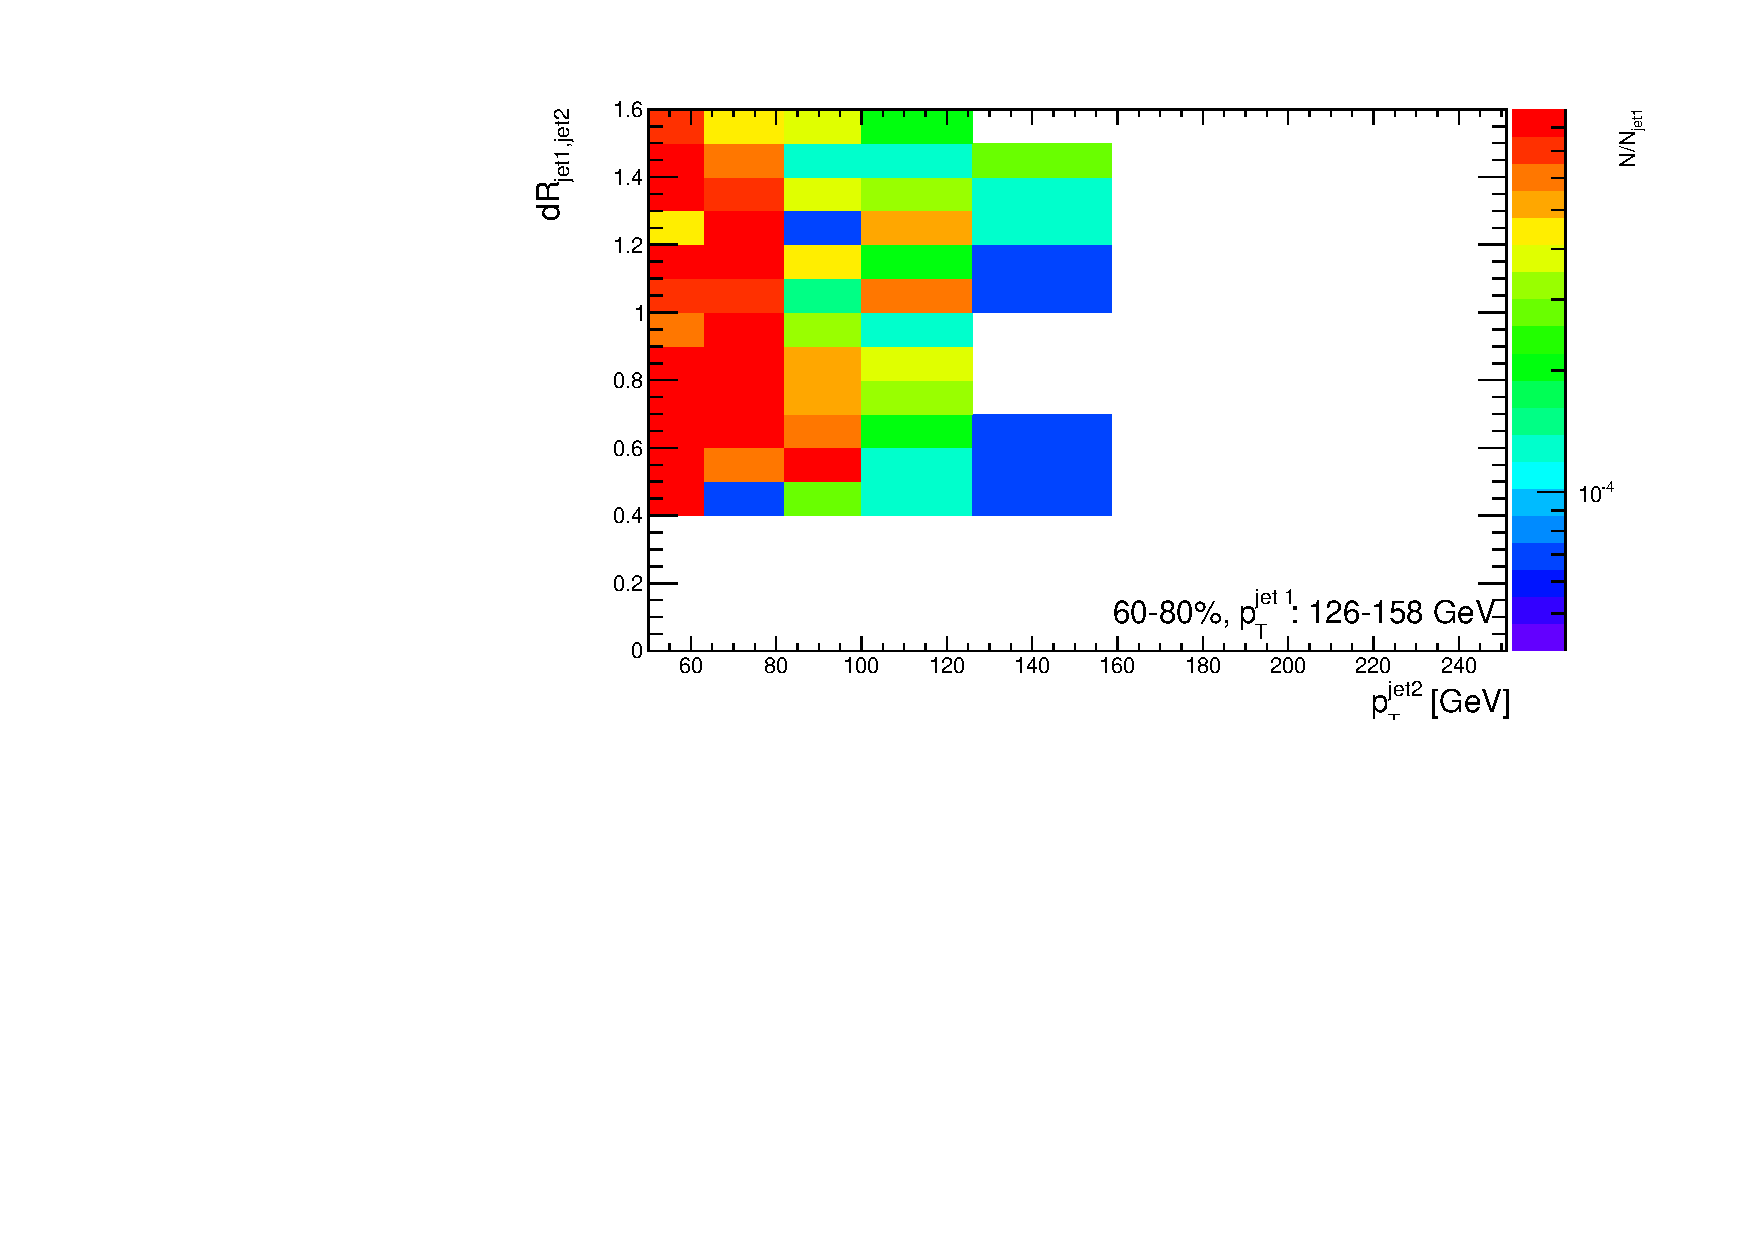
\includegraphics[width=0.45\textwidth]{figures_corrections/RdR_126_158GeV_c5.pdf} \\
%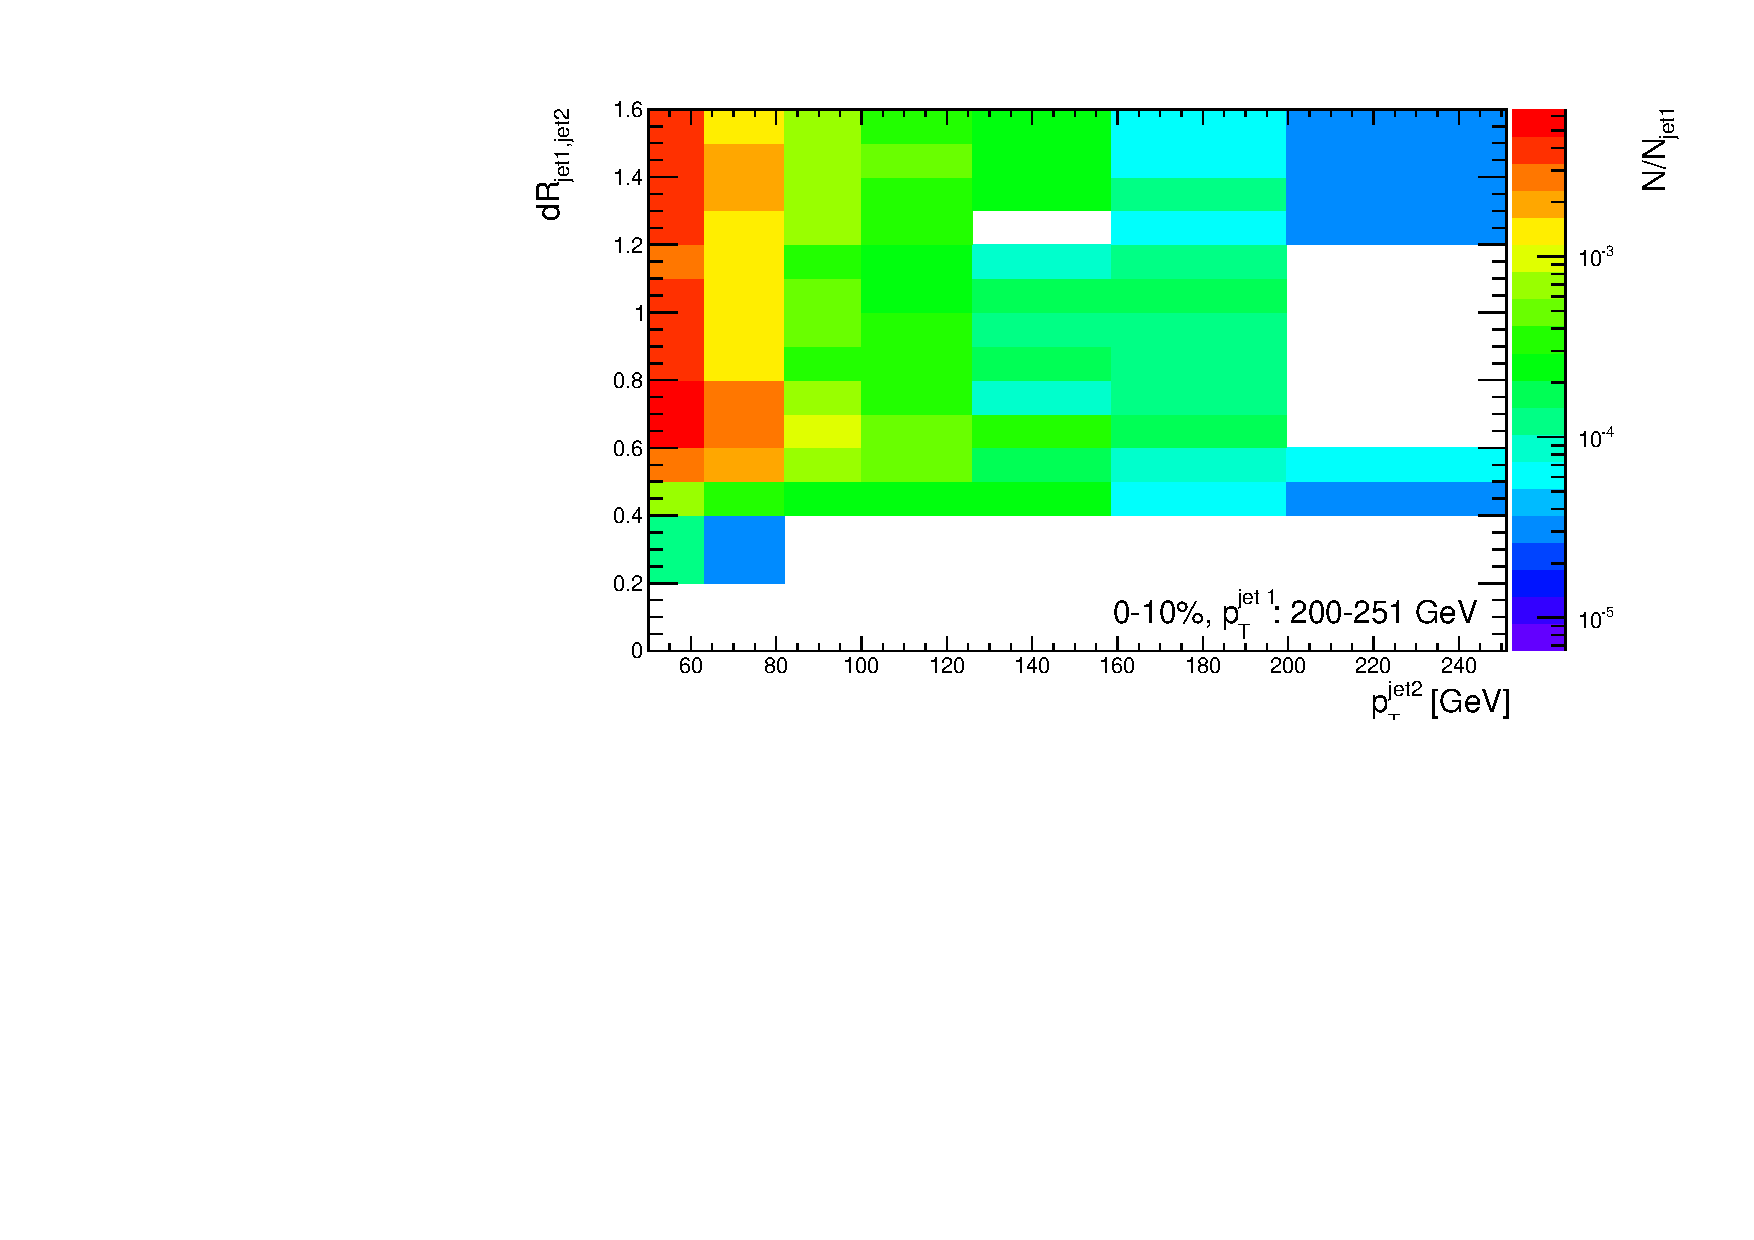
\includegraphics[width=0.45\textwidth]{figures_corrections/RdR_200_251GeV_c0.pdf} &
%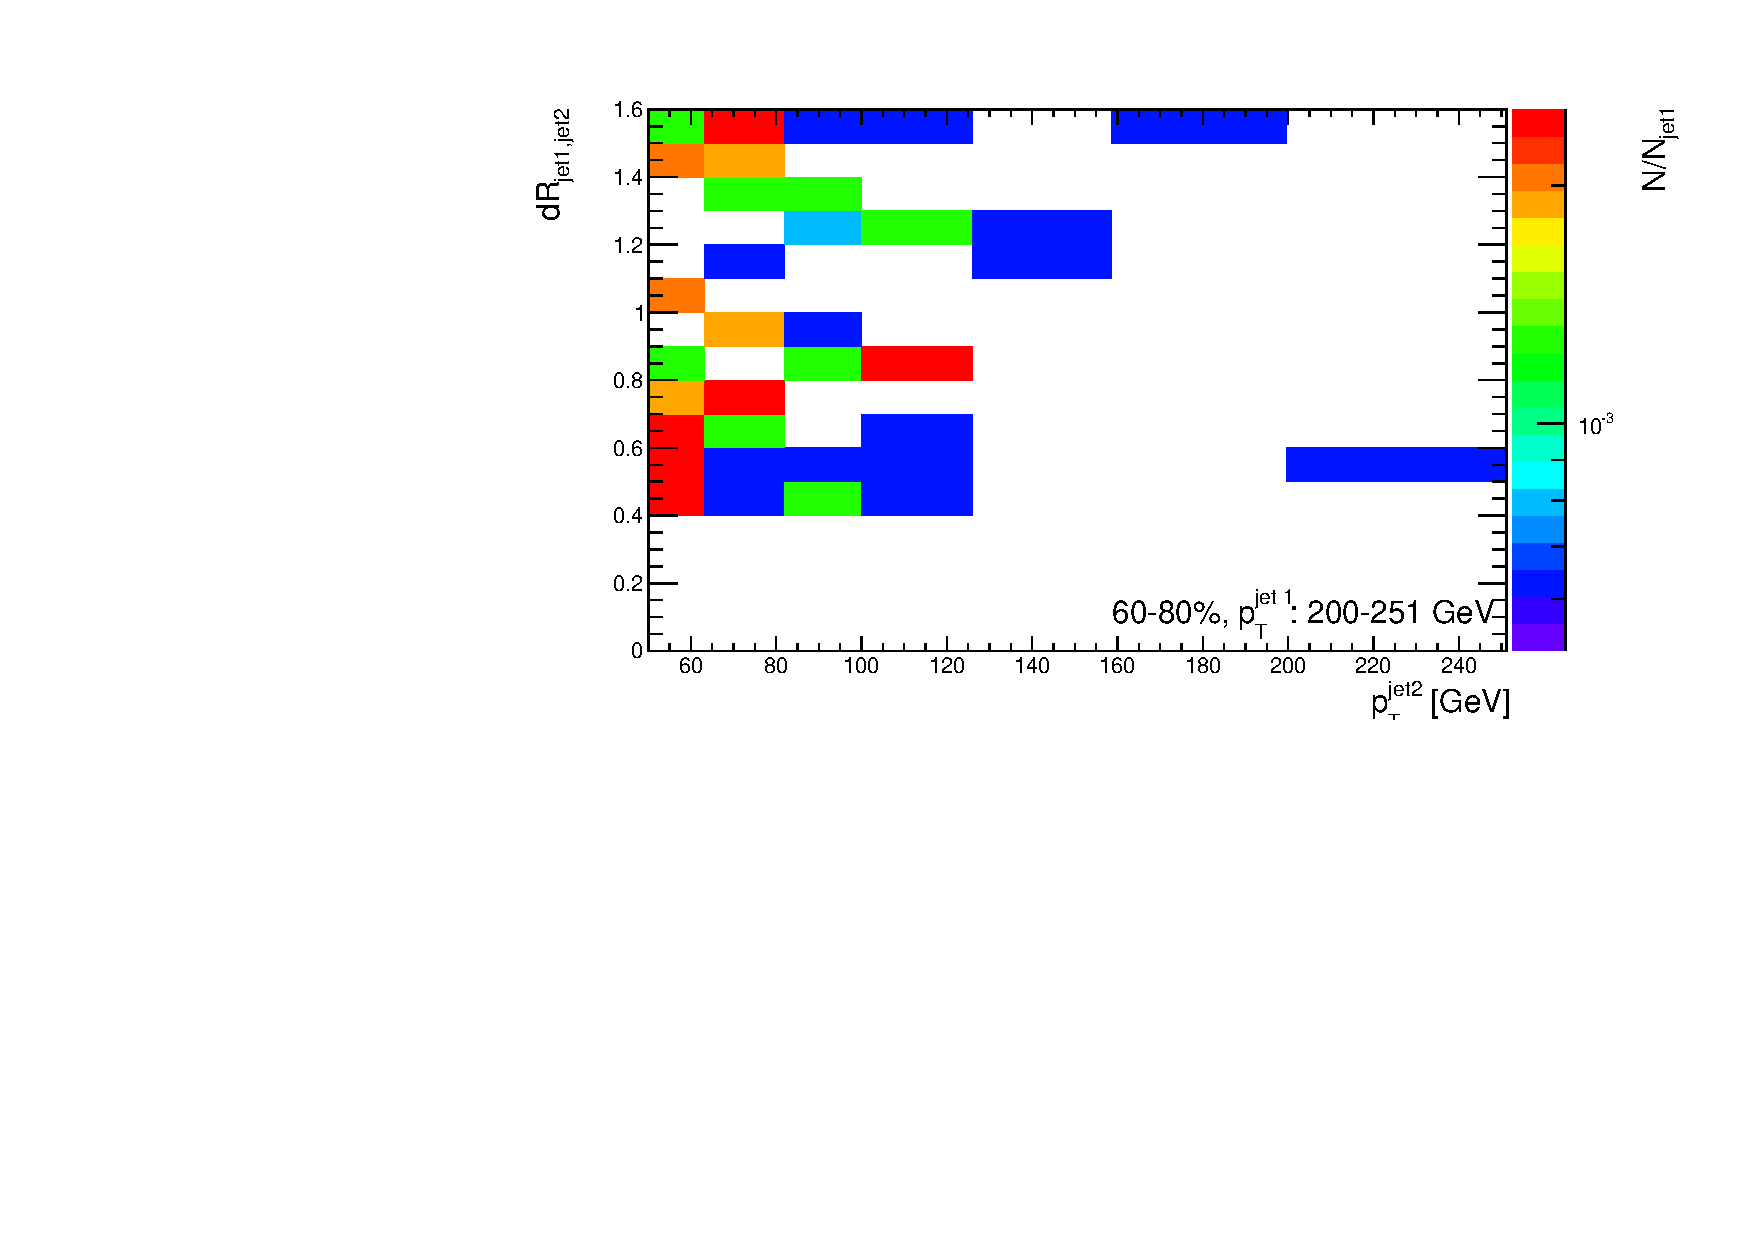
\includegraphics[width=0.45\textwidth]{figures_corrections/RdR_200_251GeV_c5.pdf} \\ 
%\end{tabular}}
%\caption{Conditional yield of jets with $\pt^{2}$ that accompany a higher \pt\ jet with $\pt^{1}$ as a function of their angular separation $\mathrm{d}R$. Distributions are presented for two different centrality bins and two different intervals of $\pt^{1}$.}
%\label{fig:RdR}
%\end{figure}  
 

\subsection{Track selection}
\label{sec:trackselection}

The track selection cuts used here follow the cuts used in~\cite{ATLAS502FFConf}. These provide a low level of fake tracks and 
a track reconstruction efficiency that is independent of the \pt\ of the jet the track is associated with.  
The cuts used here are the ``tight" cuts as described in Ref.~\cite{ref:tracktwiki} and were utilized in previous HI jet fragmentation measurements. The default tracking cuts used both in \pp\ and \PbPb\ analysis are:
\begin{itemize}
\item{ track $\pT>$~1~GeV}
\item{ track $|\eta|<$~2.5}
\item{ tracks should have at least 9 silicon hits in $|\eta|\leq1.65$}
\item{ tracks should have at least 11 silicon hits in $|\eta|>1.65$}
\item{ tracks should have at least 1 hit in IB-layer + B-layer.}
\item{tracks should have a IB-layer hit if it is expected, i.e. if the track passed an active module.}
\item{tracks should have a B-layer hit if it is expected and IB-layer hit is not expected.}
\item{ tracks should have  less than 3 holes in silicon detectors.}
\item{ tracks should have 0 holes in pixel detector.}
\item{impact parameters of track with respect to primary vertex:  $|d_0|<$$< 0.47\times \exp{(-0.15\times\pT)} + 0.19\times \exp{(0.00034\times\pT)}$~mm, $|z_0*\sin\theta|<$1.0~mm. Recommendation values are  $|d_0| < 1.5$~mm for tracks with $\pt<10$~GeV and $|d_0| < 0.2$~mm for tracks with $\pt>10$~GeV.
  	
  	This was chosen to guarantee a smooth behavior of the $d_{0}$ parameter as a function of track momentum. }
\item{ An additional cut on the track to jet \pT\ ratio is included. All tracks with 
\begin{equation}
\pTtrk >  \ptjet + \sqrt{ (3 \times \sigma_{\mathrm{JER}}(\ptjet))^2 + (3 \times \sigma_{\mathrm{TMR}}(\pTtrk))^2} 
\end{equation}
are rejected from the analysis. Where the $TMR$ stands for track momentum resolution. The purpose of this cut is to reduce the fake rate by removing tracks that have significantly larger \pt\ than the jet that they belong to.
 }
\end{itemize}

 

A tighter tracking selection is used for systematic studies (``tight+'' cuts).  These cuts include all of the default
cuts plus a 3$\sigma$ cut on the significance of the $d_0$ and $z_0 \sin\theta$.
Figures~\ref{fig:trkdataMCcomp_pp}-\ref{fig:trkdataMCcomp_pbpb_highpt}
shows comparisons of the data and MC tracking quantities in \pp\ and
\pbpb\ collisions, respectively, for different track \pT\ intervals.  Overall the MC describes the data well. A ~20\% discrepancy is observed for low impact parameters. The discrepancy is present far from the values of corresponding tracking cuts. A small overall shift of the $z0$ distribution is observed in MC samples. This difference is caused by the allowance of a small difference in the $z$ position of the primary vertex in the MC overlay procedure. However this has negligible impact on the analysis as the overall quality requirement on the pointing in the $z0$ is 1~mm. Furthermore, Fig.~\ref{fig:trkdataMCcomp_pbpb_highpt} shows the same comparison for high \pt\ tracks. All the comparisons of distributions show the same qualitative features as seen at lower \pt\ with improving pointing with increasing track \pt. The comparison of the reconstructed \pttrk\ with the generated
kinematics for tracks passing these cuts is shown in Fig.~\ref{fig:momres_pp}.

\begin{figure}
\centering{
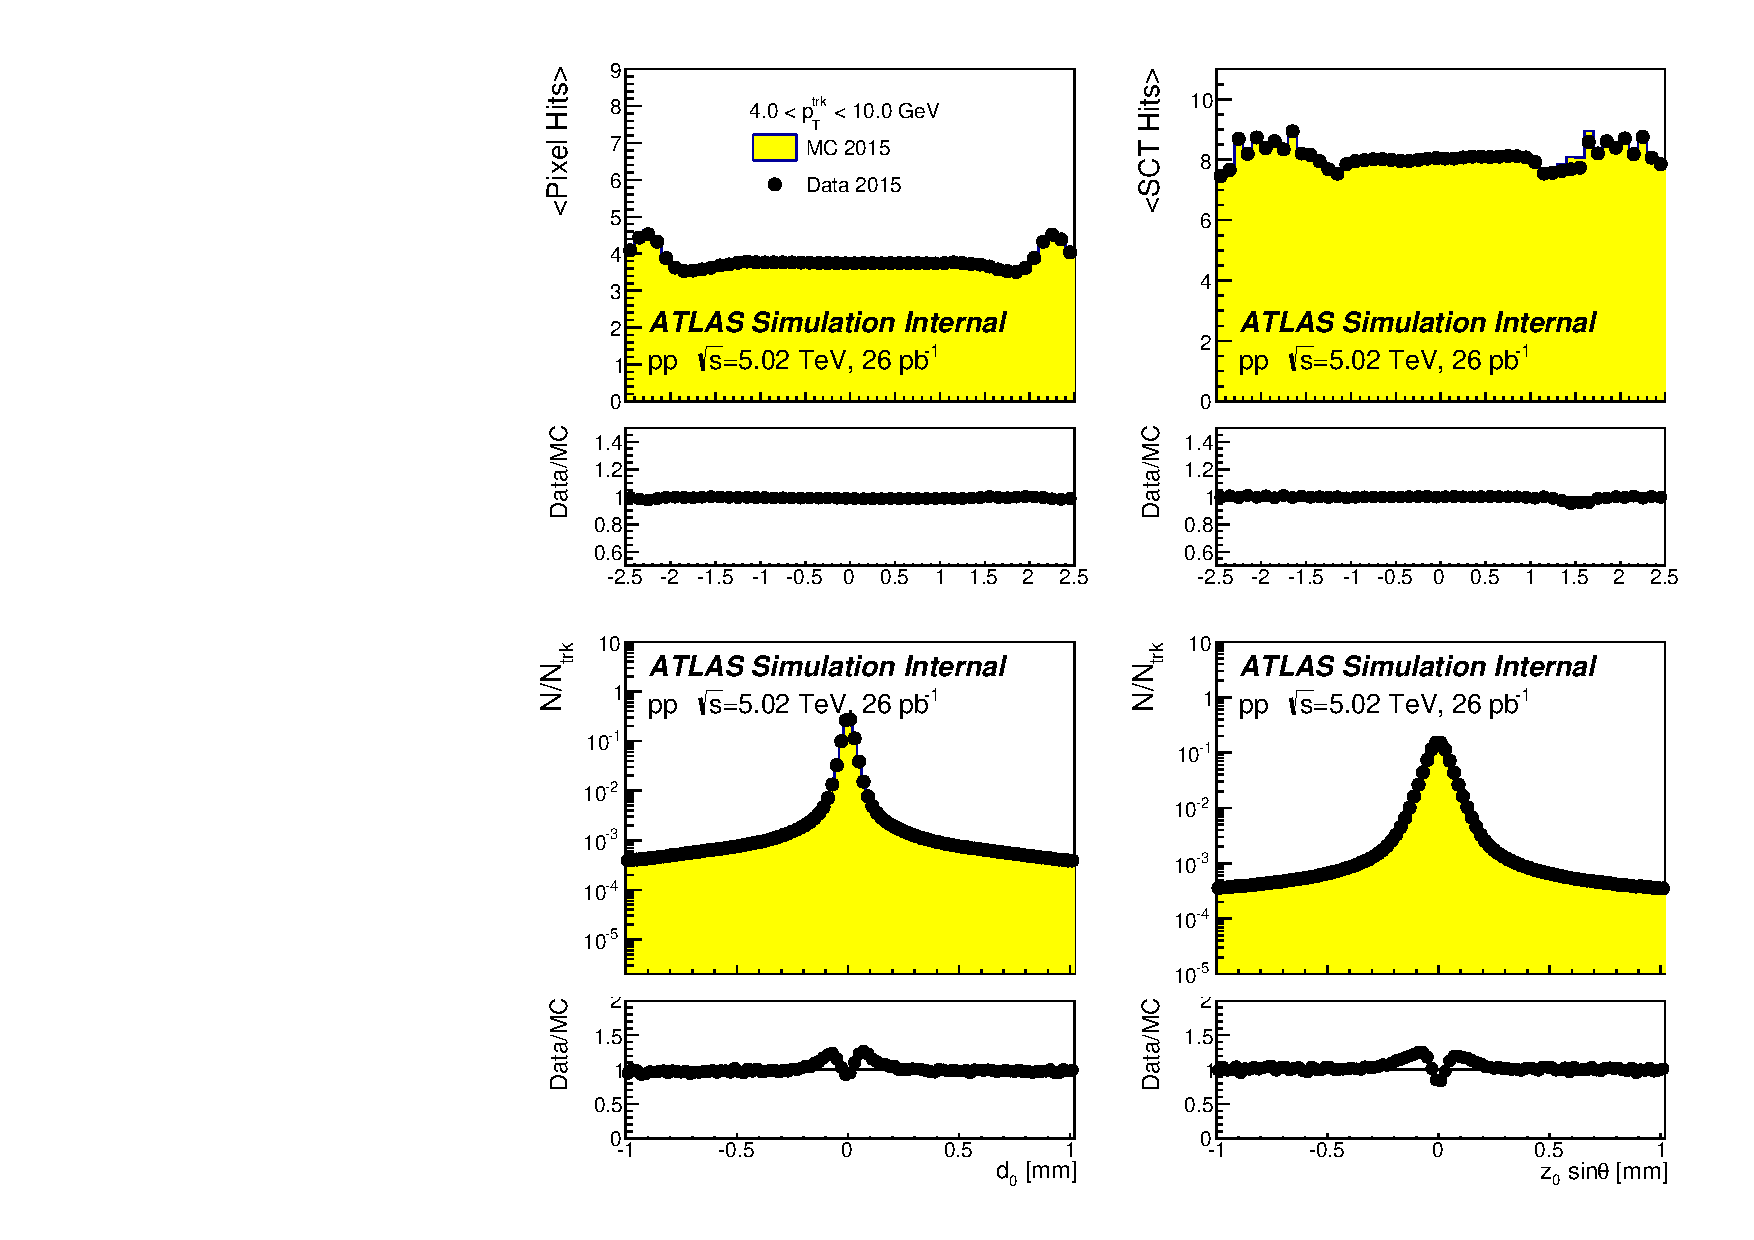
\includegraphics[width=0.75\textwidth]{figures_performance/TrkPerforPlots_5TeV_pp.pdf} }
\caption{Track quantity comparison between data (points) and MC (yellow histogram) in \pp\ collisions.  
Tracks are selected to have 4.2~$<\pttrk<$~10~GeV. Below each direct data and MC overlay is the 
corresponding data to MC ratio.  The quantities compared are: average number of pixel hits as a function
of $\etatrk$ (top left), average number of SCT hits as a function of $\etatrk$ (top right),
and number of tracks, $N_{\mathrm{trk}}$, normalized $d_0$ (bottom left), and $z_0 \sin\theta$ distributions (bottom right).}
\label{fig:trkdataMCcomp_pp}
\end{figure}

\begin{figure}
\centering{
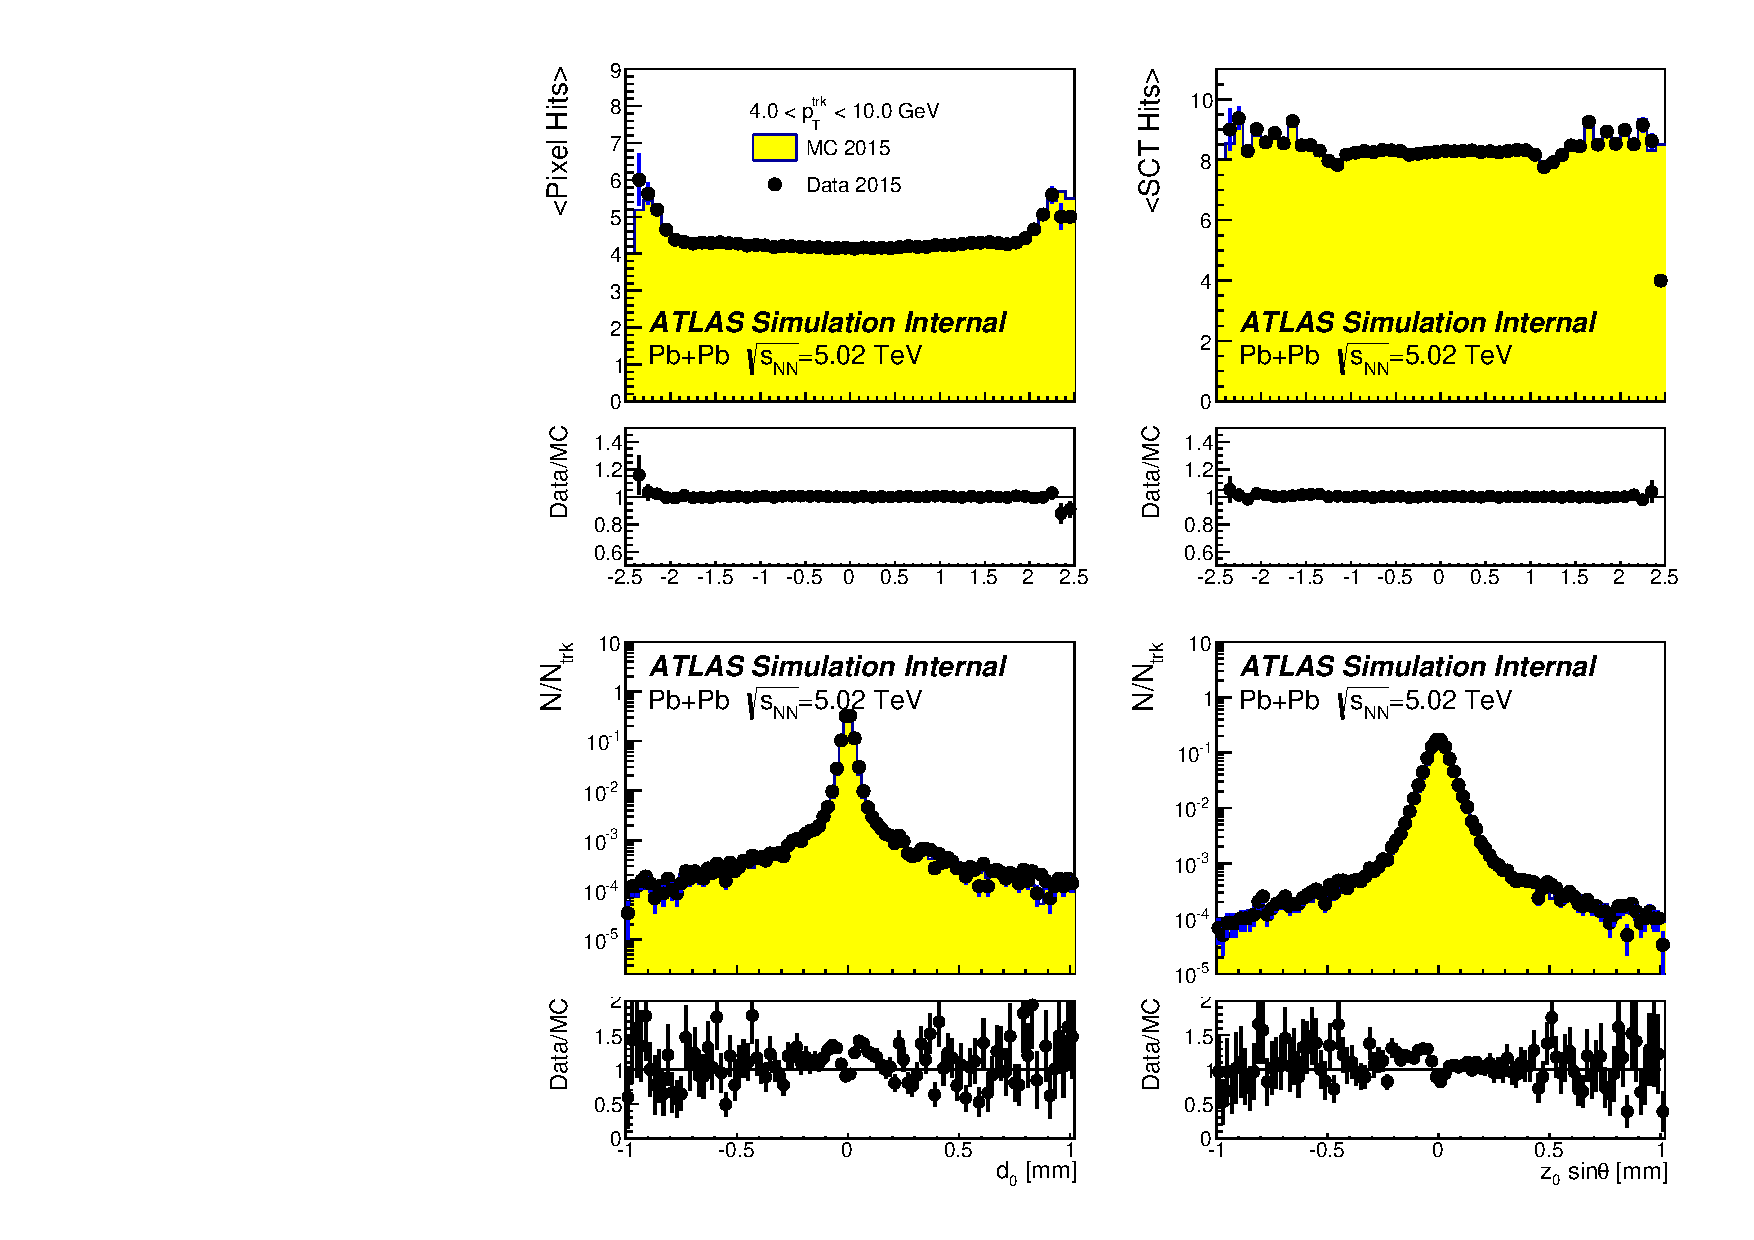
\includegraphics[width=0.75\textwidth]{figures_performance/TrkPerforPlots_PbPb_pt4p2_10p0GeV.pdf} }
\caption{Track quantity comparison between data (points) and MC (yellow histogram) in 0-10\%
   central \pbpb\ collisions.  
Tracks are selected to have 4.2~$<\pttrk<$~10~GeV. Below each direct data and MC overlay is the 
corresponding data to MC ratio.  The quantities compared are: average number of pixel hits as a function
of $\etatrk$ (top left), average number of SCT hits as a function of $\etatrk$ (top right),
track $d_0$ (bottom left), and track $z_0 \sin\theta$ (bottom right).}
\label{fig:trkdataMCcomp_pbpb}
\end{figure}

\begin{figure}
\centering{
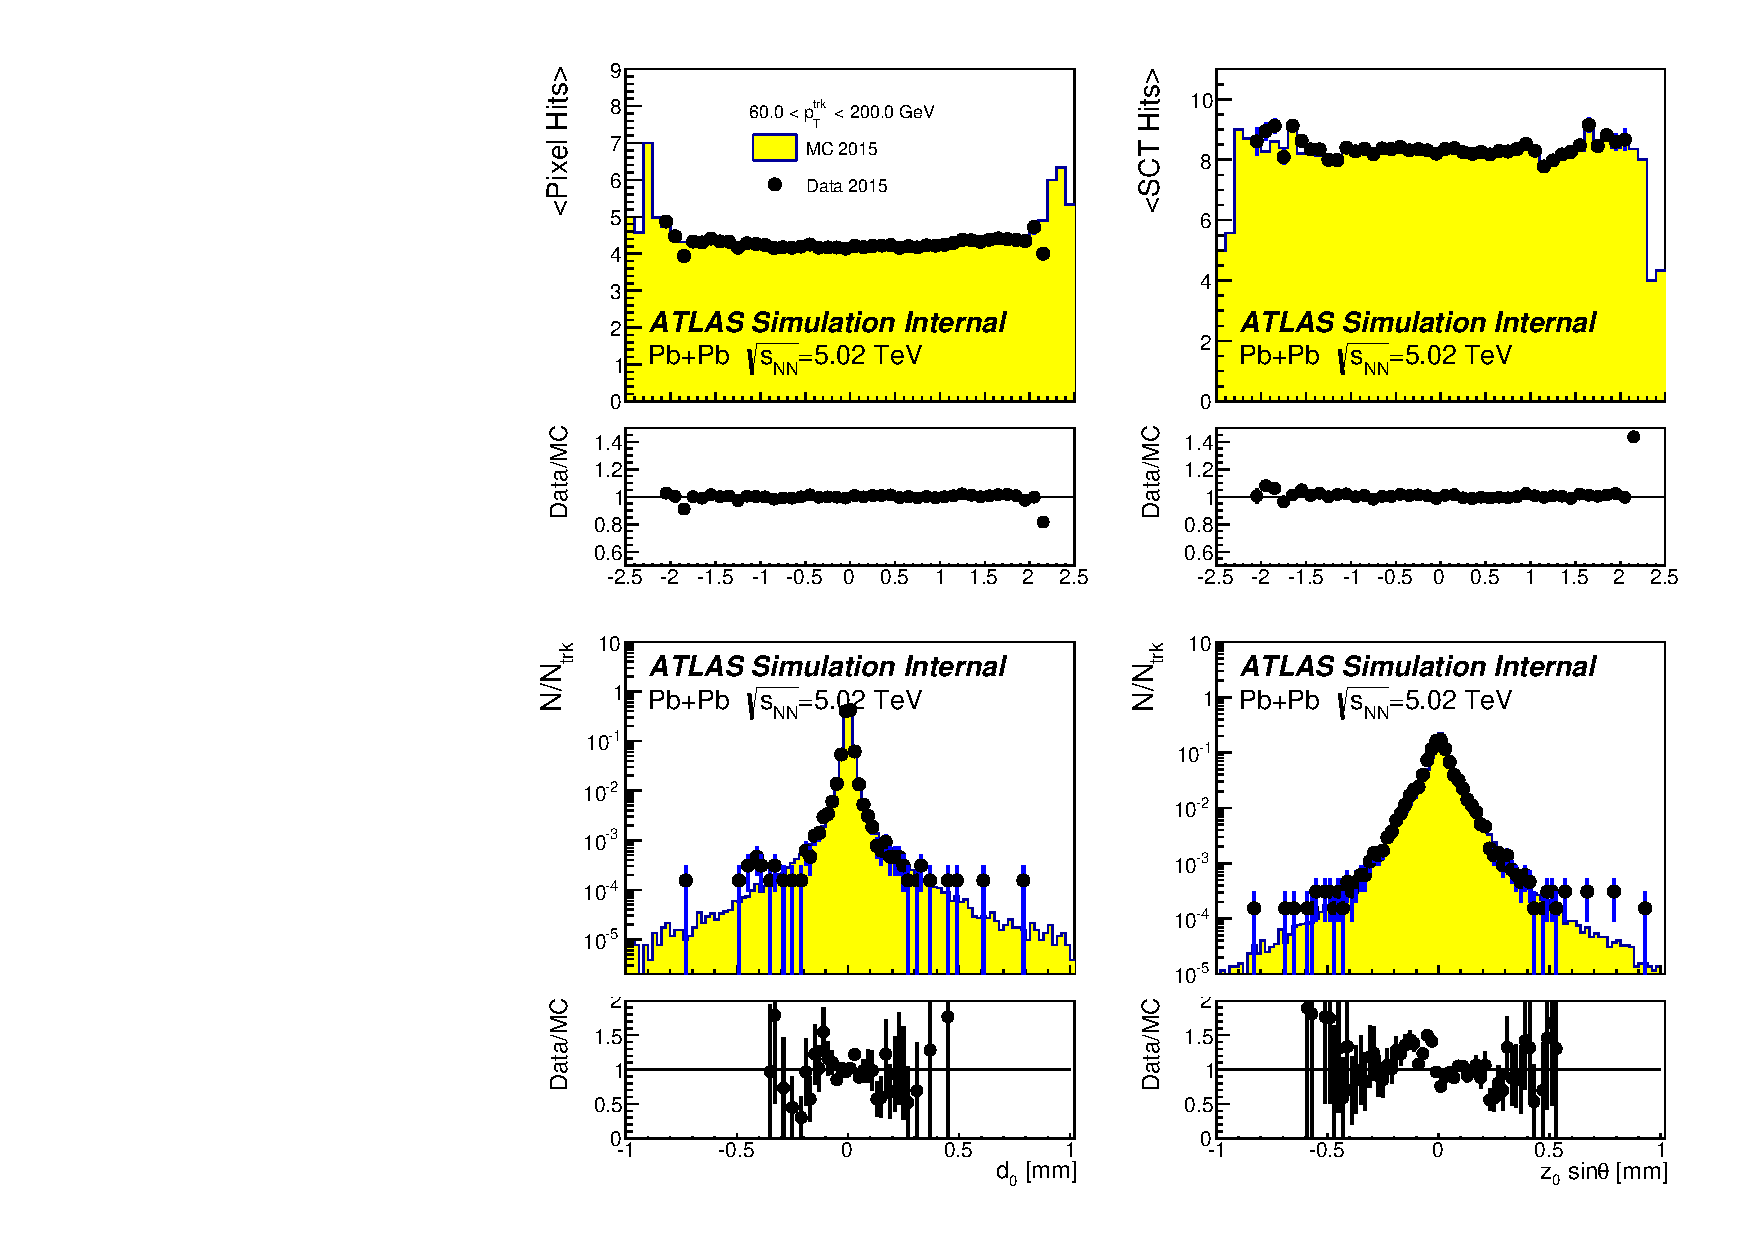
\includegraphics[width=0.75\textwidth]{figures_performance/TrkPerforPlots_PbPb_pt60_200GeV.pdf} }
\caption{Track quantity comparison between data (points) and MC (yellow histogram) in \pbpb\ collisions inclusive in collisions centrality.  
Tracks are selected to have 60~$<\pttrk<$~200~GeV and to originate from jet with \pt\ in the interval from 251 to 316 GeV. Below each direct data and MC overlay is the 
corresponding data to MC ratio.  The quantities compared are: average number of pixel hits as a function
of $\etatrk$ (top left), average number of SCT hits as a function of $\etatrk$ (top right),
track $d_0$ (bottom left), and track $z_0 \sin\theta$ (bottom right).}
\label{fig:trkdataMCcomp_pbpb_highpt}
\end{figure}


\begin{figure}
\centering{
\begin{tabular}{cc}
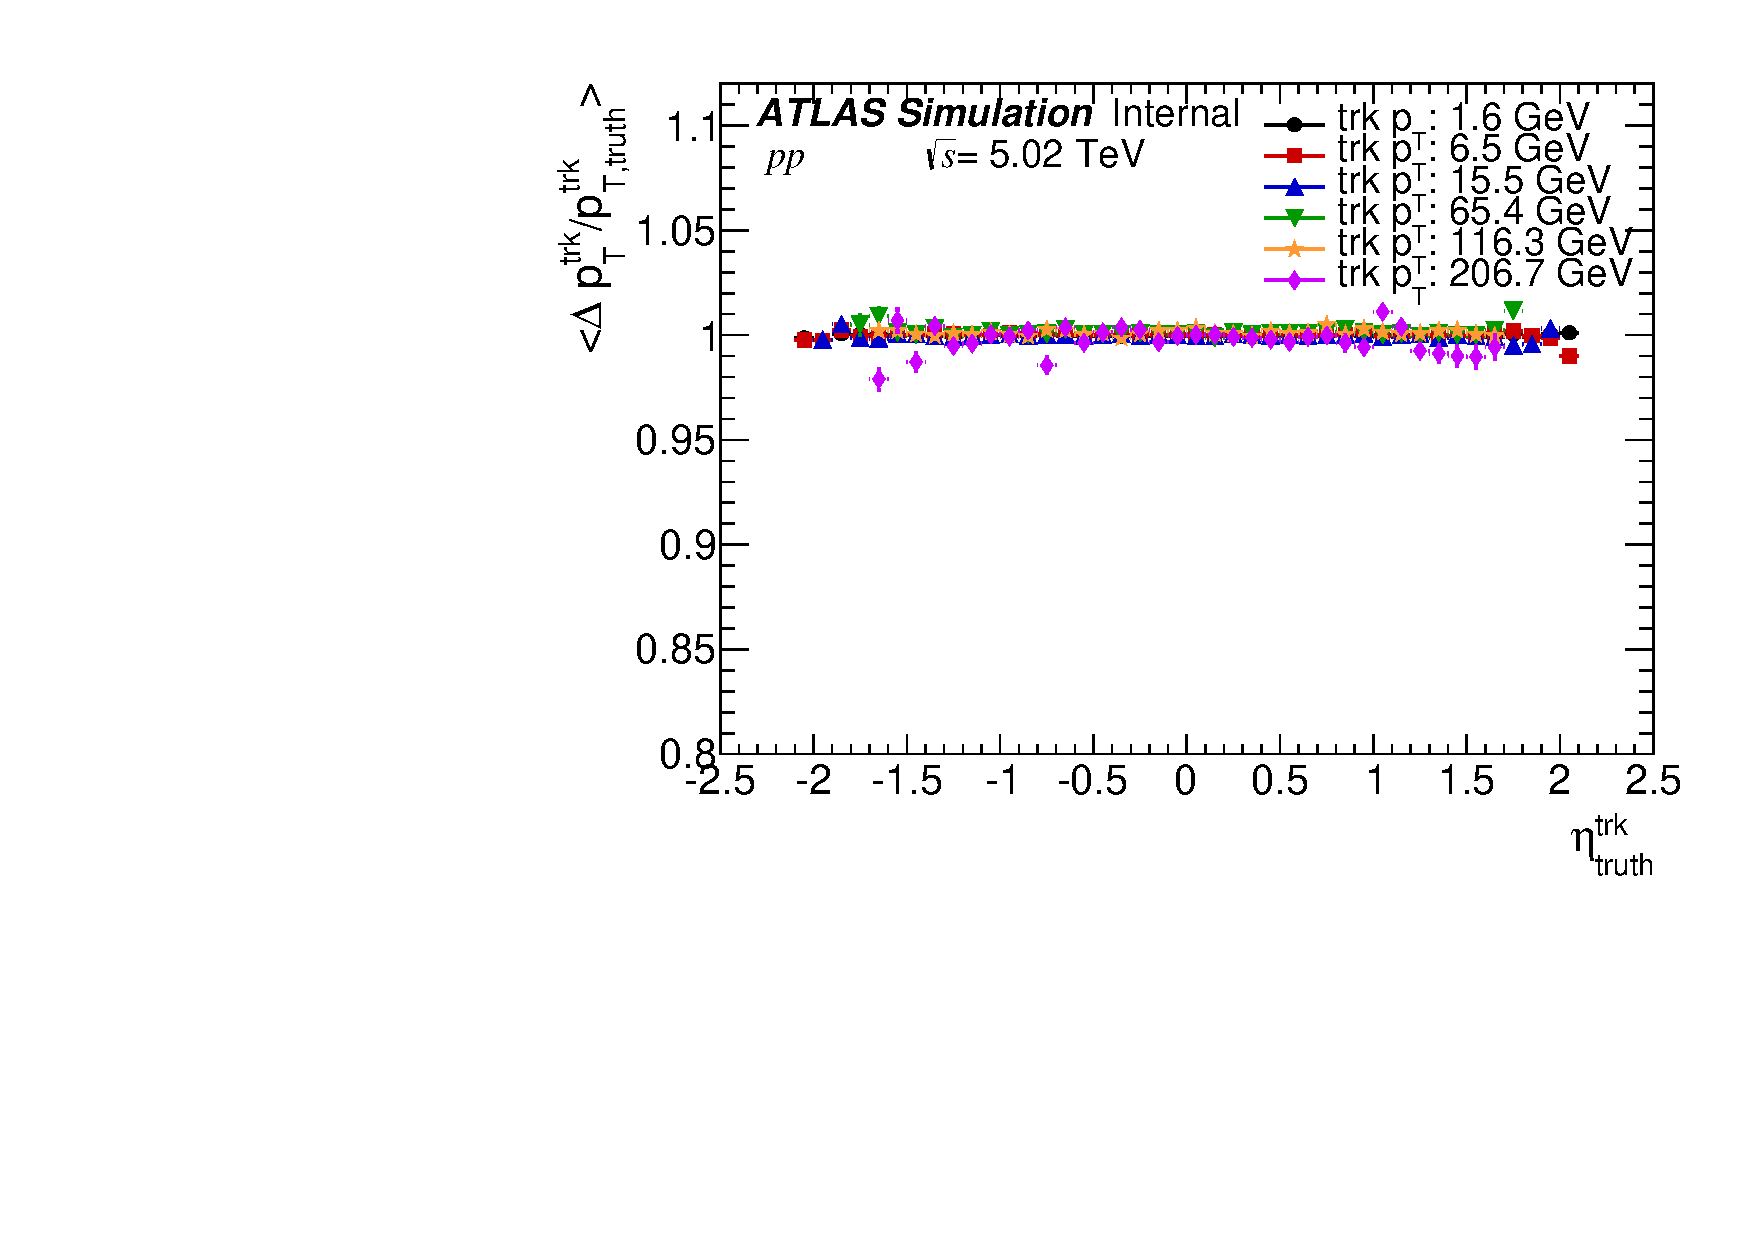
\includegraphics[width=0.45\textwidth]{figures_performance/scale_v_eta_pp.pdf} &
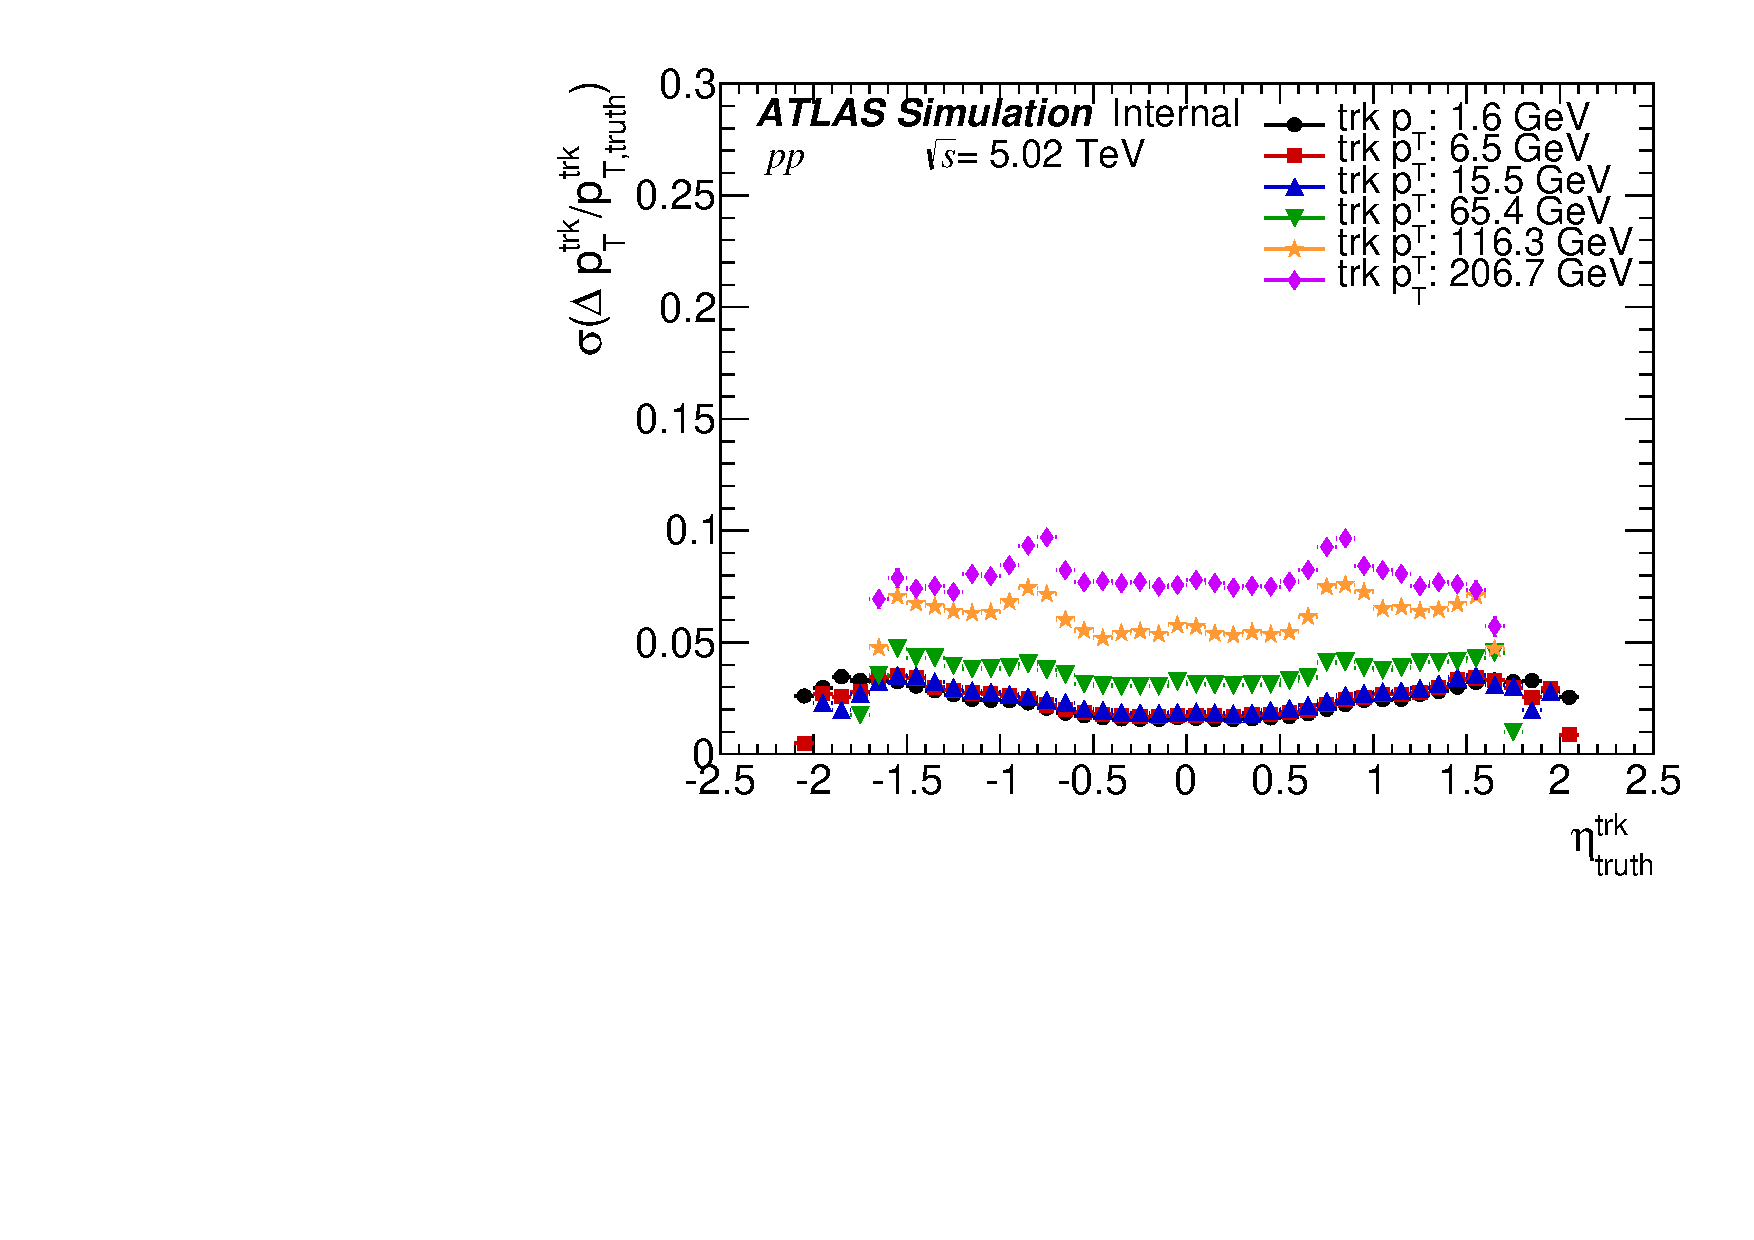
\includegraphics[width=0.45\textwidth]{figures_performance/resolution_v_eta_pp.pdf} \\ 
\end{tabular}}
\caption{(left) Comparison of the generated and reconstructed track \pt\ as a function of \etatrktruth\ for 
five track \pttrktruth\ selections. 
(right) Track momentum resolution as a function of \etatrktruth\ for five \pttrktruth\ selections.
Both plots are for \pp\ MC.  
All tracks shown in this plot have passed the 2015 default tracking cuts defined in this section.}
\label{fig:momres_pp}
\end{figure}



Figure~\ref{fig:ppcutflow_eta} presents the impact of individual tracking requirements in terms of the ratio of the number of tracks that pass given cut and the total number of reconstructed tracks in \pp\ MC. The study is presented as a function of track pseudorapidity in two different track \pT\ intervals and as a function of track \pT\ in two different pseudorapidity intervals. The highest rejection for low \pT\ tracks is provided by the cut on $d_{0}$ pointing. At high \pT\, the dominant effect is seen from the requirement on the number of silicon hits. Similarly, Fig.~\ref{fig:PbPbcutflow_eta} presents the impact of individual tracking requirements in \PbPb\ MC. The difference between the impact of individual cuts can be attributed to a different setting of the tracking algorithm and to the overall increase of the track multiplicity as the number of rejected tracks does not linearly scale with the multiplicity that enters the denominator.       

\begin{figure}
\centering{
\begin{tabular}{cc}
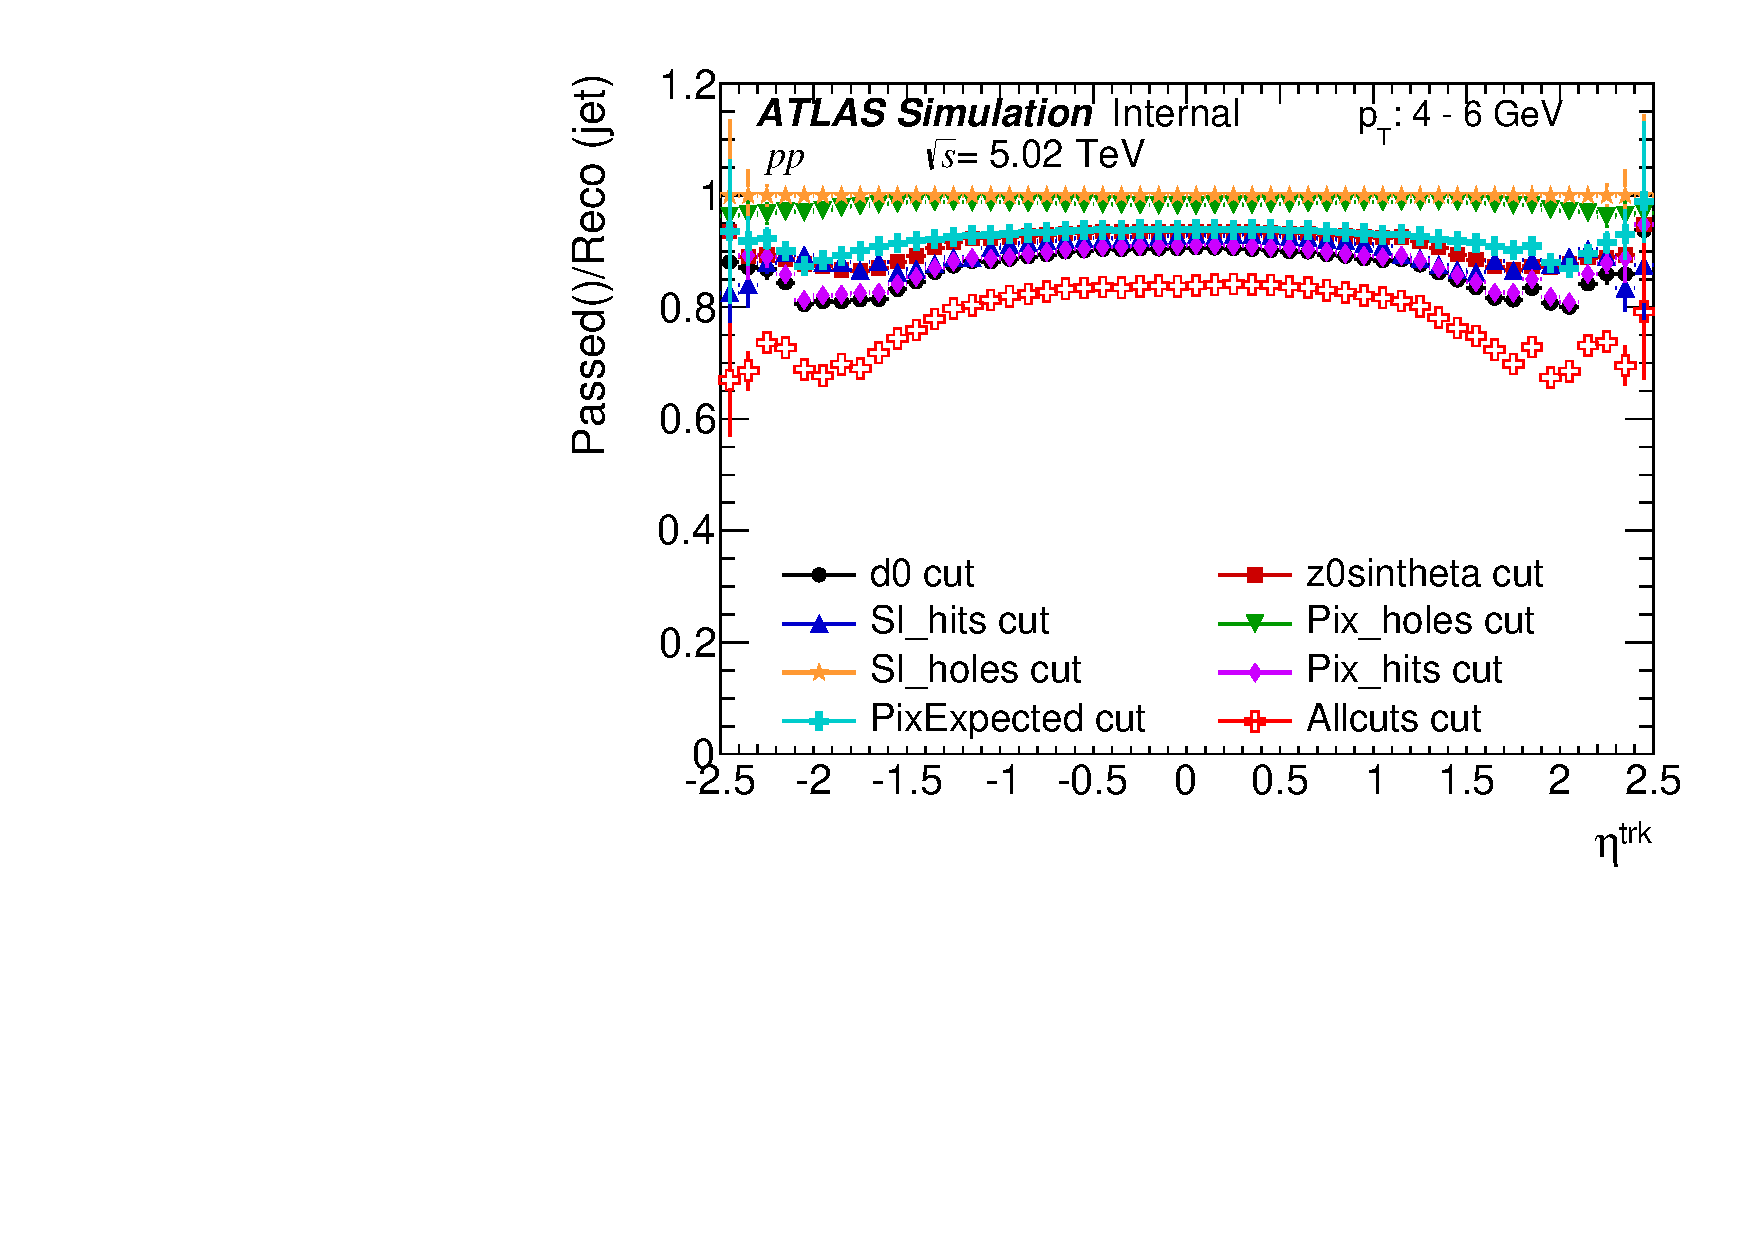
\includegraphics[width=0.45\textwidth]{figures_performance/cut_flow_RecoNorm_MC_pT_4_6_jet.pdf} &
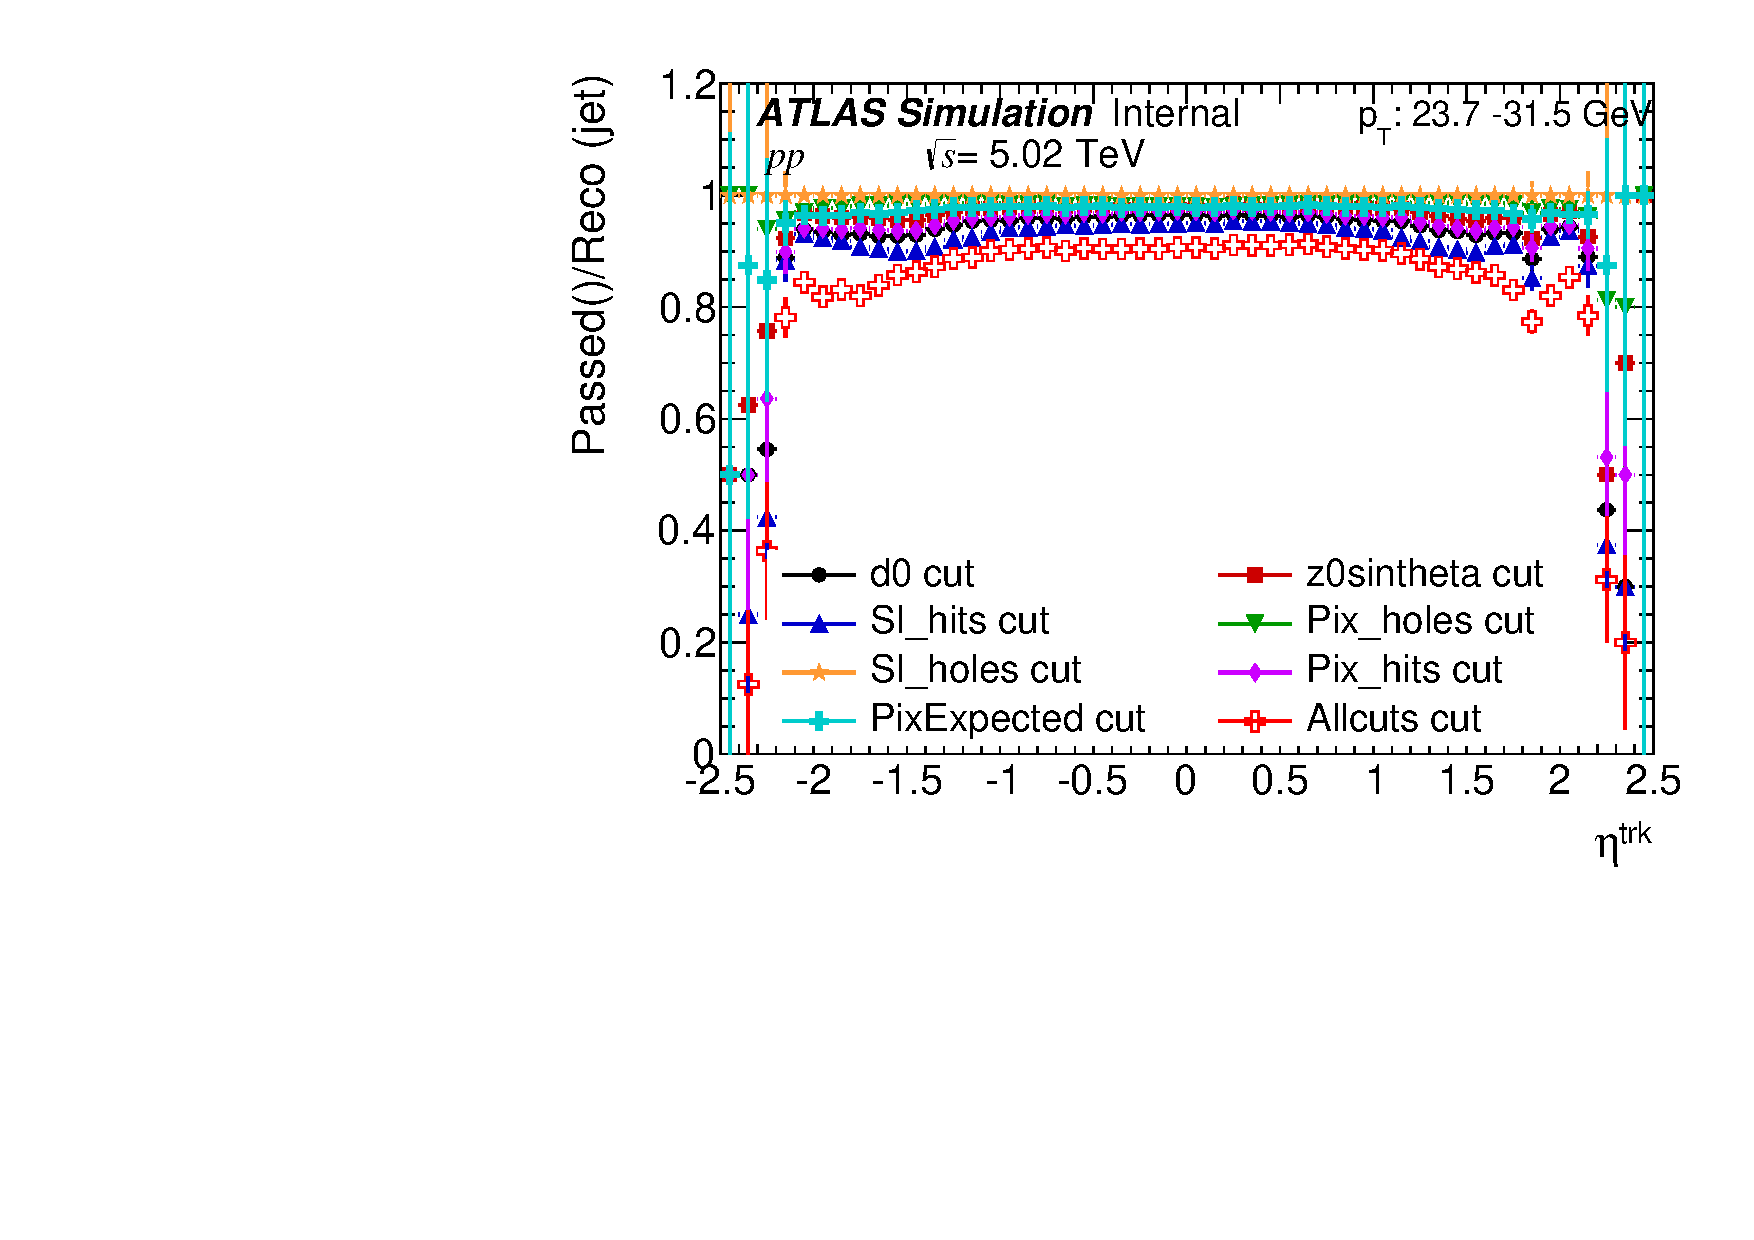
\includegraphics[width=0.45\textwidth]{figures_performance/cut_flow_RecoNorm_MC_pT_23p7_31p5_jet.pdf} \\
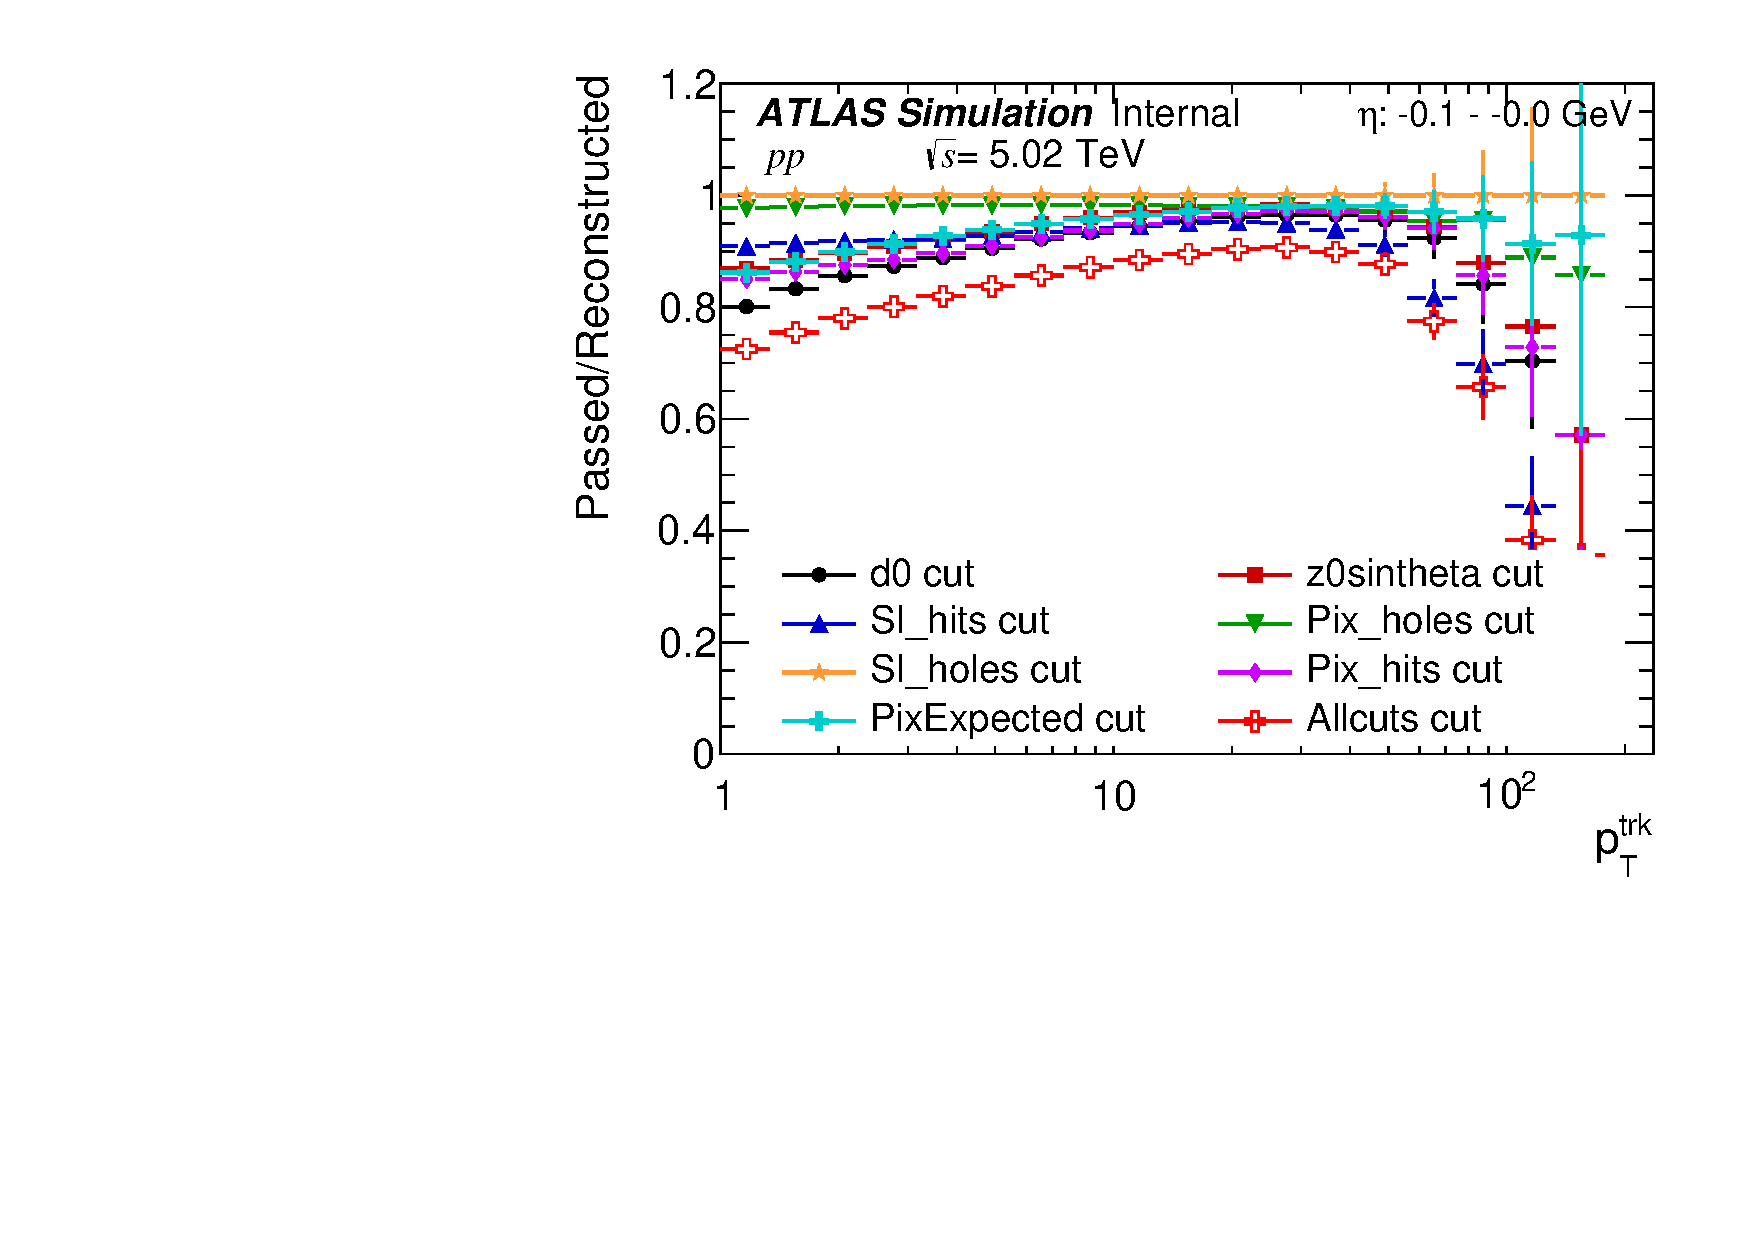
\includegraphics[width=0.45\textwidth]{figures_performance/cut_flow_RecoNorm_MC_eta_0p05_jet.pdf} &
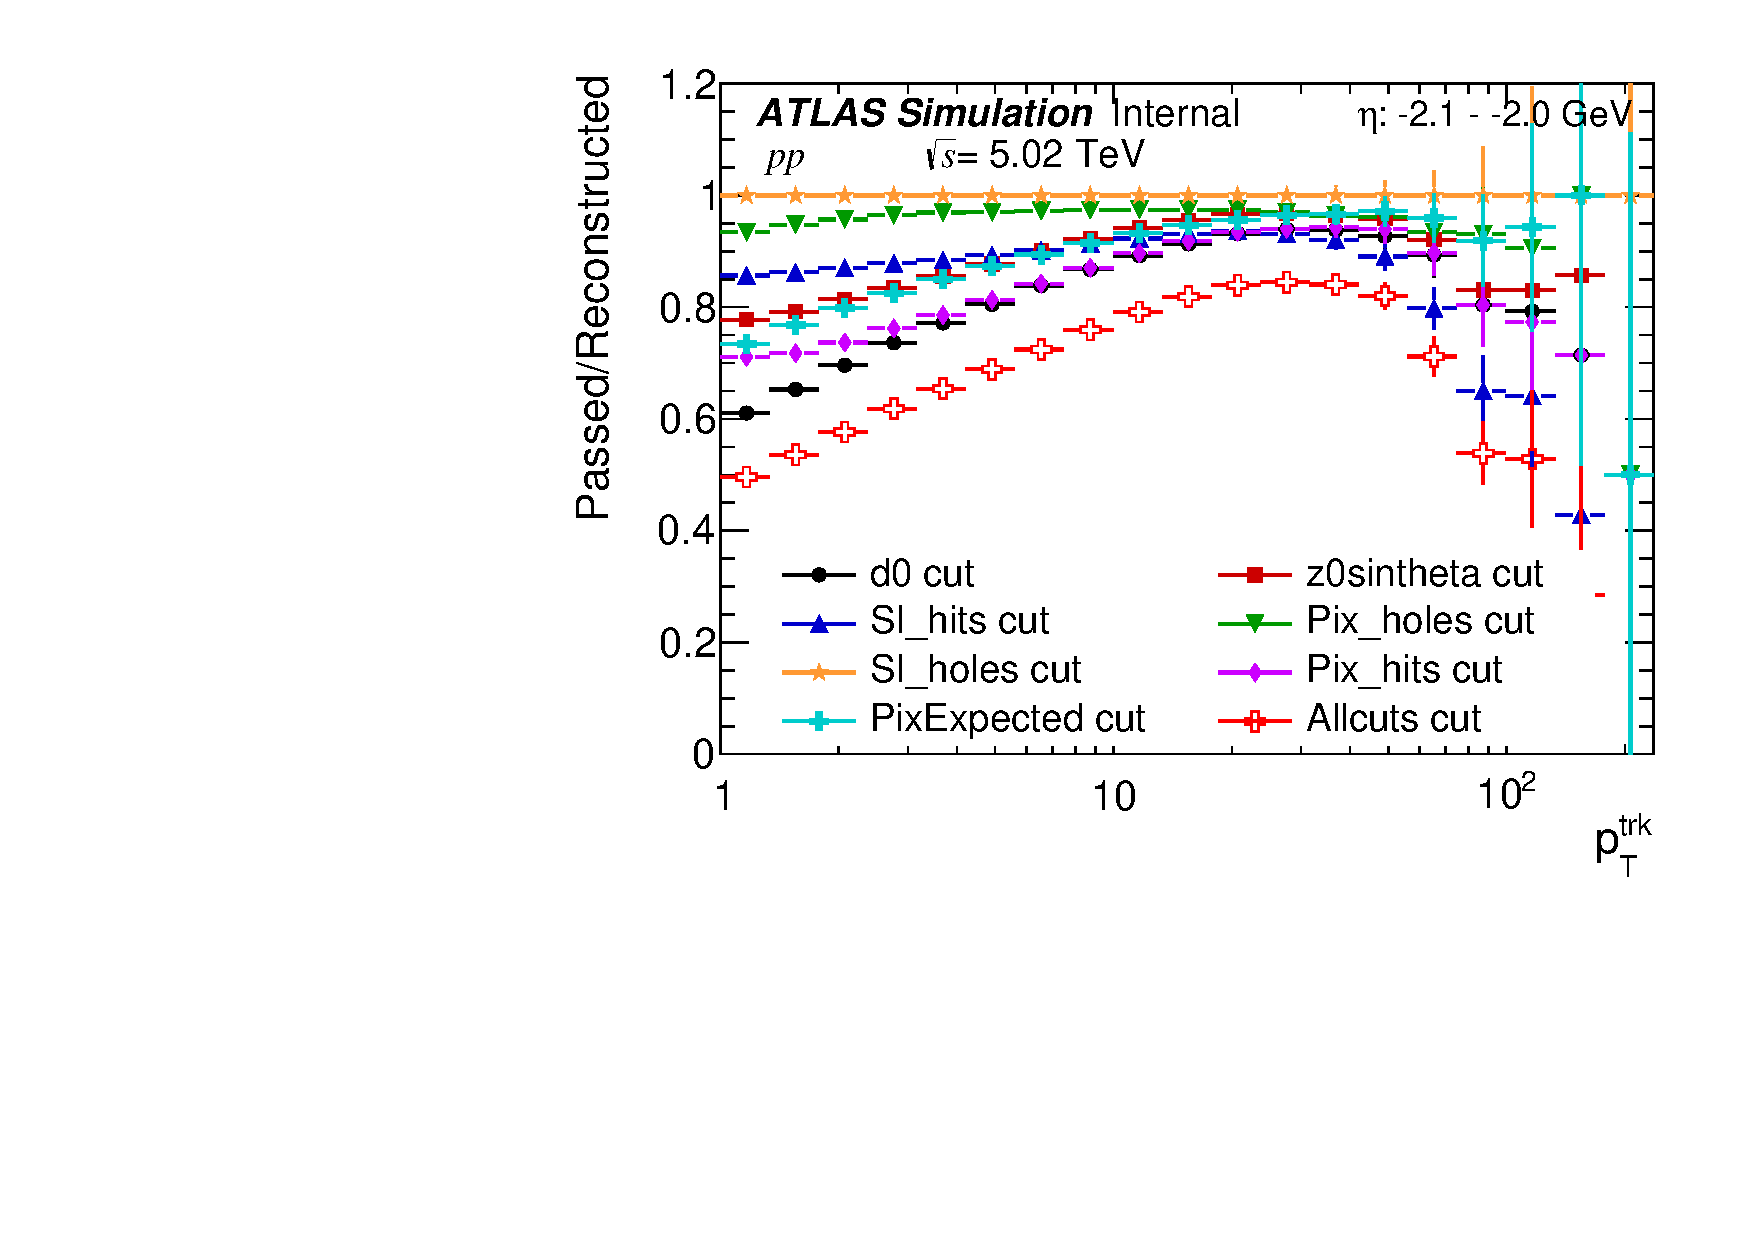
\includegraphics[width=0.45\textwidth]{figures_performance/cut_flow_RecoNorm_MC_eta_2p05_jet.pdf} \\
\end{tabular} }
\caption{The impact of each cut applied individually in the \pp\ MC 
to the starting collection of tracks, as a function of
\etatrk (top) for 4.6~$>\pttrk>$~1.3~GeV (left) and for 23.7~$<\pttrk<$~31.5~GeV and as a function of track \pT\ for two different pseudorapidity intervals (bottom).  The final combination of all cuts is shown as well.}
\label{fig:ppcutflow_eta}
\end{figure}

\begin{figure}
\centering{
\begin{tabular}{cc}
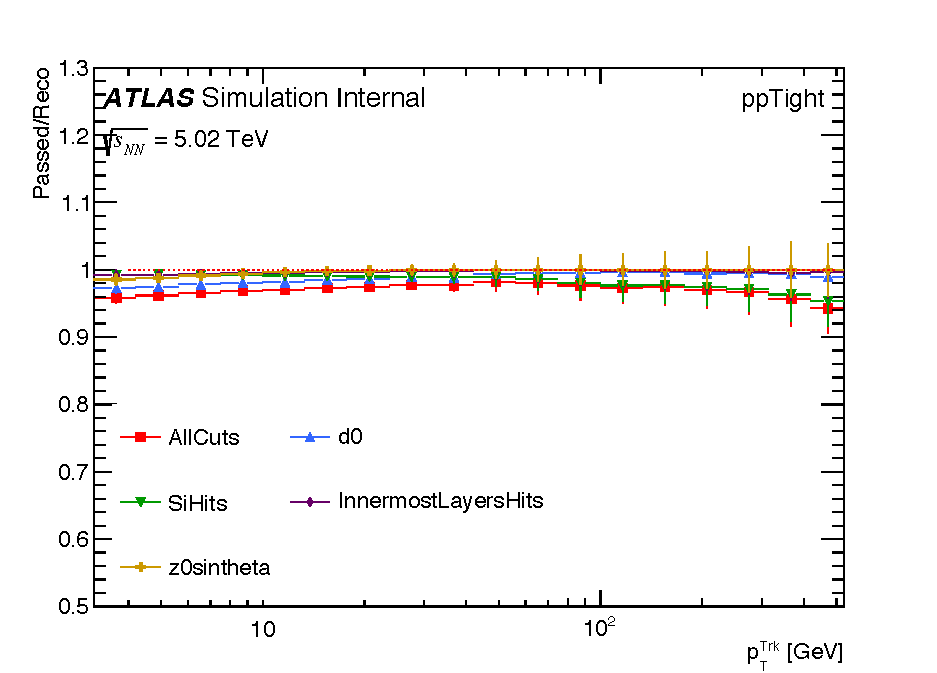
\includegraphics[width=0.45\textwidth]{figures_performance/PbPb_cutflow_pptight.pdf} &
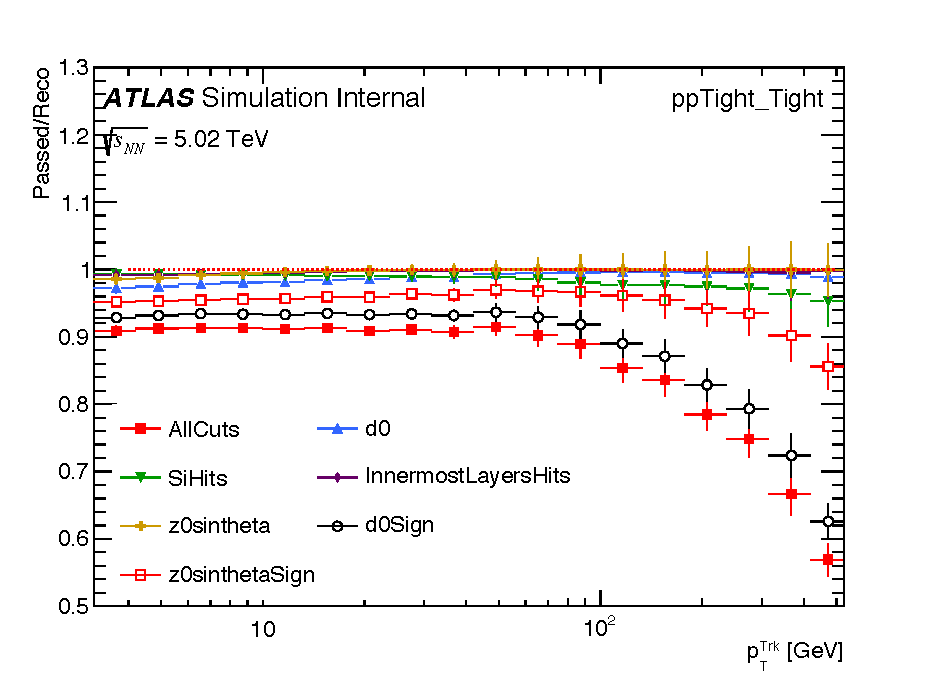
\includegraphics[width=0.45\textwidth]{figures_performance/PbPb_cutflow_pptight_tight.pdf} \\
\end{tabular} }
\caption{The impact of each cut applied individually in the \PbPb\ MC 
to the starting collection of tracks, as a function of the track \pT\ inclusive in collision centrality for the default and the tight set of tracking requirements. The final combination of all cuts
is shown as well.}
\label{fig:PbPbcutflow_eta}
\end{figure}

\subsection{Track momentum correction}
\label{Sec:Trackmomentumcorrection}
Specific correction is needed for track momentum in 5~TeV \pp\ and \PbPb\ data to account for miss-alignment introduced in the track reconstruction. The sign charge dependent momentum scale shift was observed in \pp\ data when the transverse momentum of muons reconstructed using muon spectrometer was compared to the transverse momentum of muons from the inner detector. The difference as a function of muon momentum can be seen in Fig.\ref{Fig:ChMomentumScale}. The correction to track \pt\ as a function of track $\eta$ and track $\phi$ is applied through sagitta bias maps introduced in InDetTrackSystematicsTools-00-00-19~\cite{TrackingRec}.

\begin{figure}[h]
\centerline{
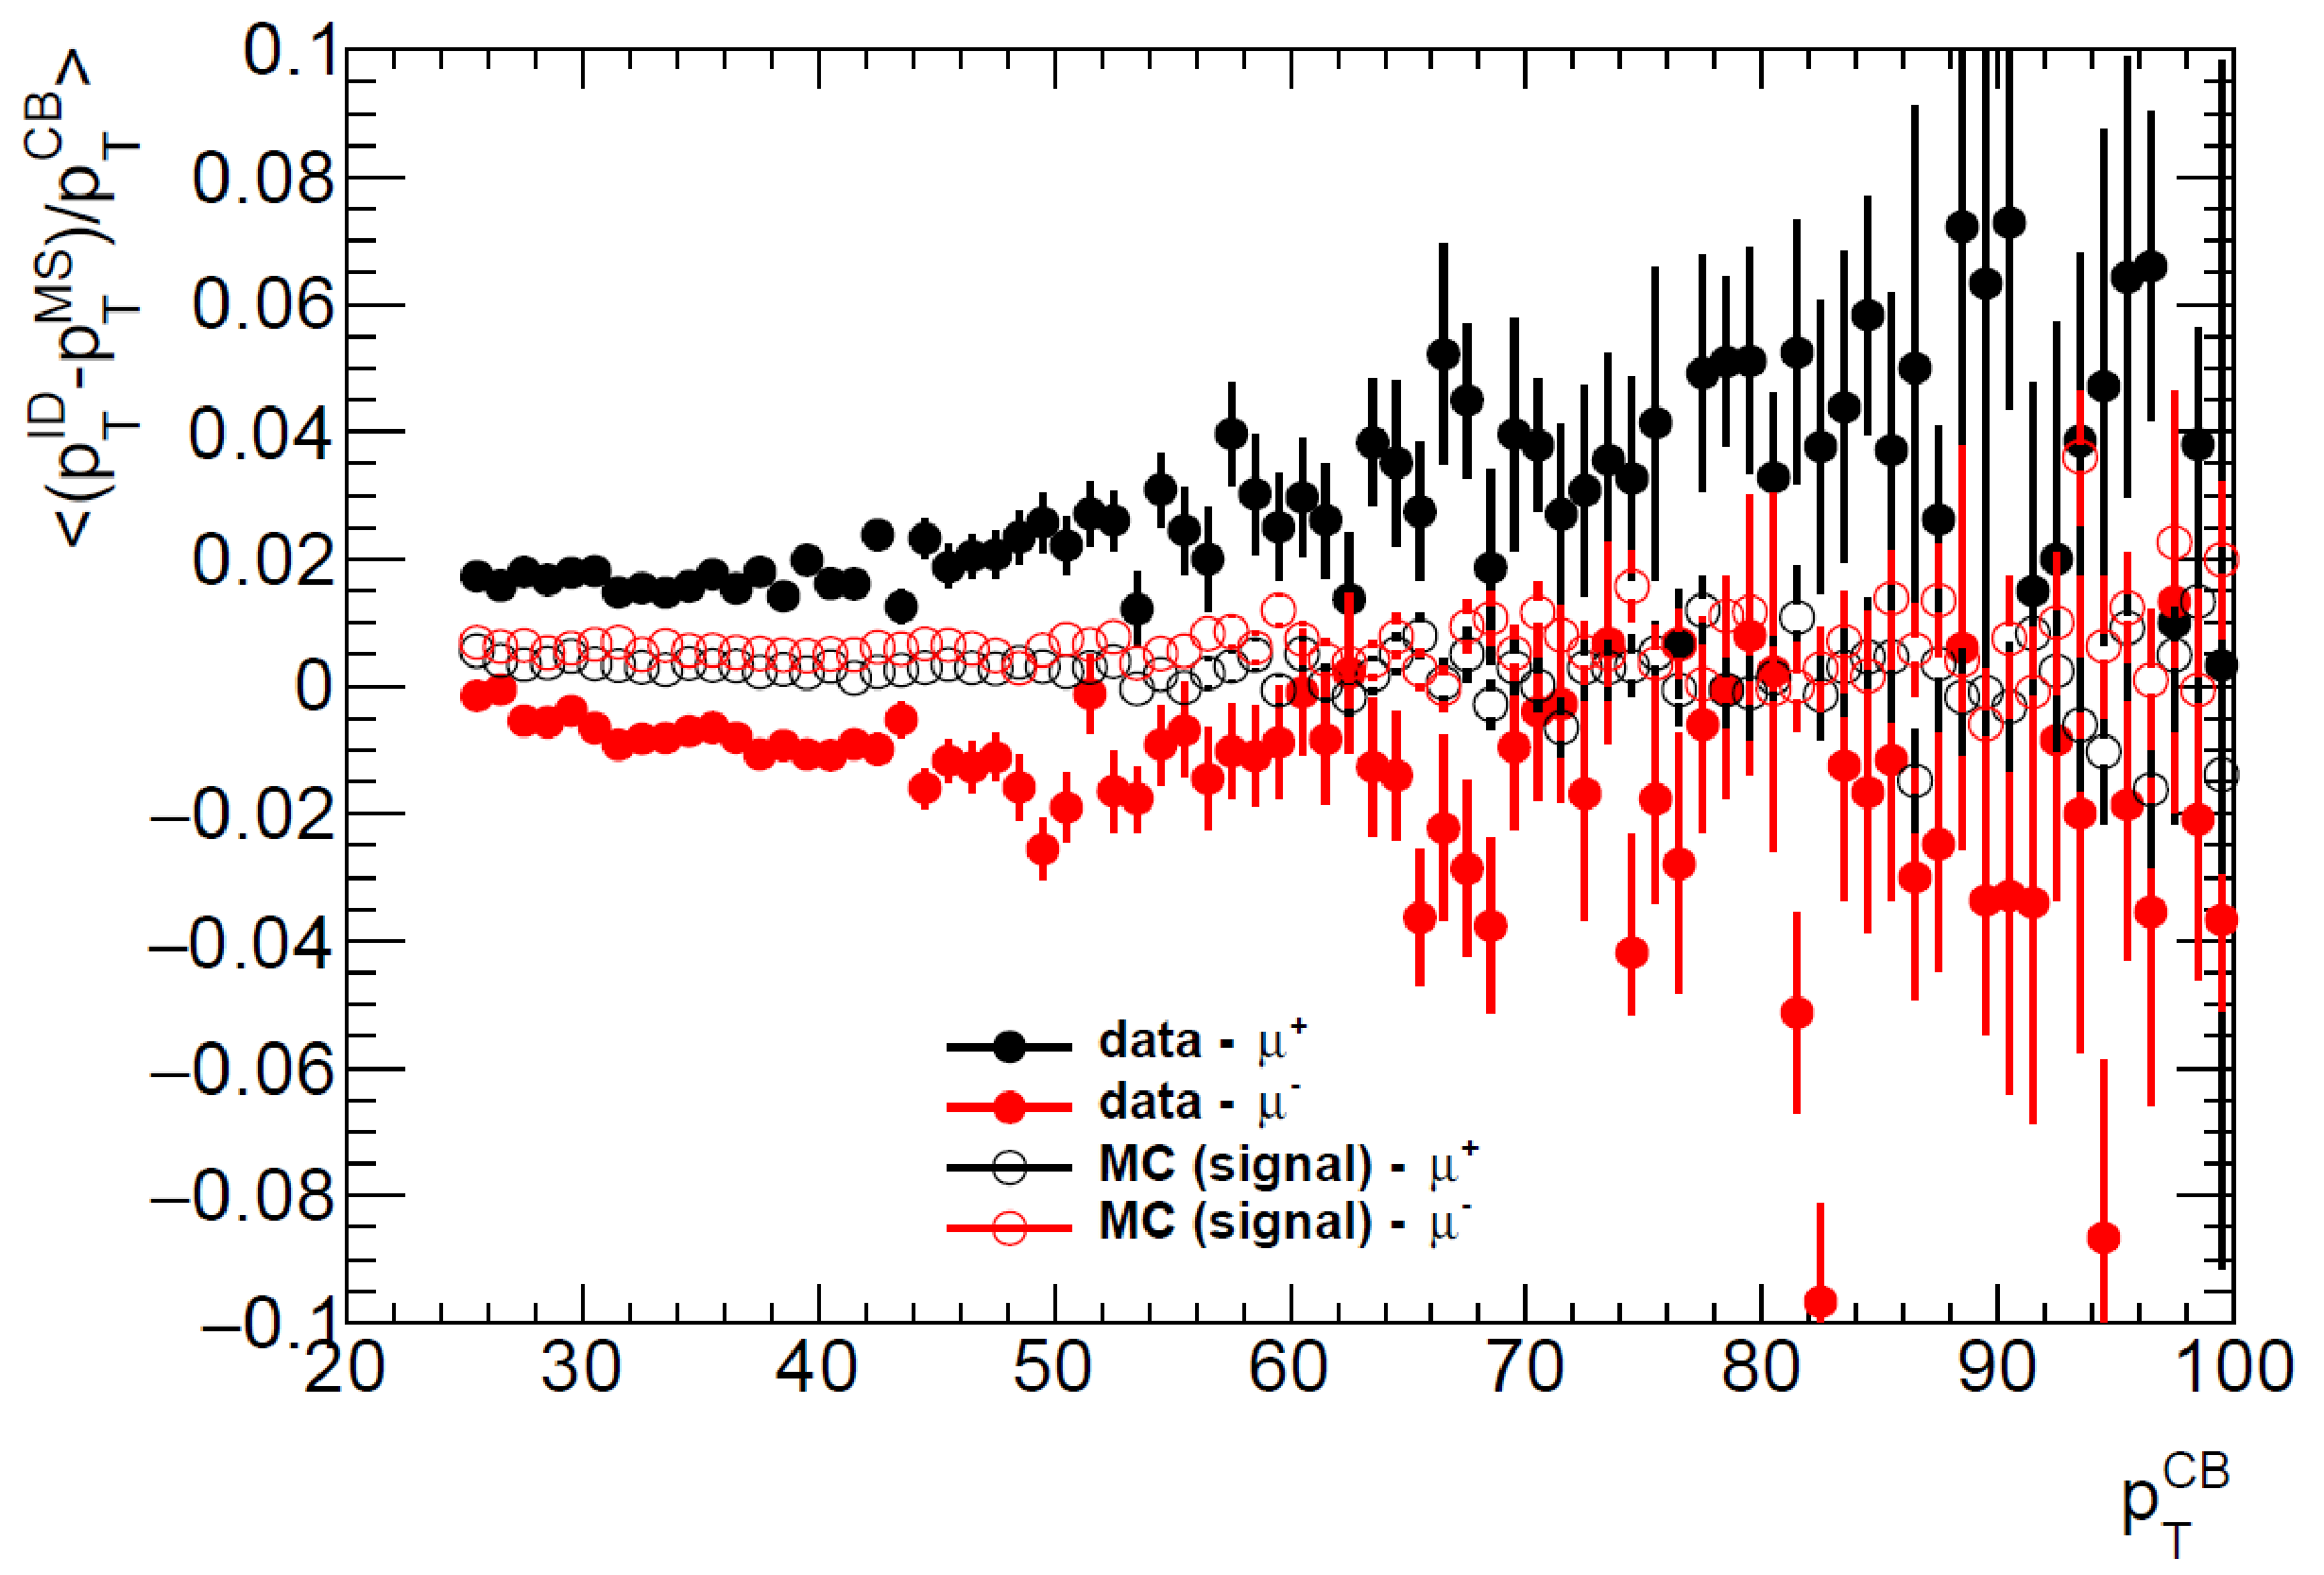
\includegraphics[width=0.75\textwidth]{figures_corrections/MuonPerf.pdf}
}
\caption{Comparisons of track momentum scale of positive and negative muons reconstructed using muon spectrometer and inner detector. The muon traverse momentum evaluated from muon spectrometer (MC) is compared by that evaluated using the inner detector (ID) and the relative scale is normalized by the momentum that uses both detectors (CB). \cite{Bold:2194917}}
\label{Fig:ChMomentumScale}
\end{figure}

%\clearpage


\subsection{Track reconstruction efficiency}
\label{sec:trackreco}

The track reconstruction efficiencies are evaluated by using MC tracks. The tracking reconstruction efficiency is defined as the ratio between the number of primary truth charged particles that are reconstructed and the total number of primary truth charged particles in the given \pt\ and $\eta$ bin. Primary particles are defined as particles with a mean lifetime $\tau > 0.3 \times 10^{-10}$~s either directly produced in \pp\ interactions or
from subsequent decays of particles with a shorter lifetime. All other particles are considered to be secondary.  Tracks are required to pass all the tracking cuts imposed on the data. 

Matching between the reconstructed and the truth track is done via a cut on $mc_{\mathrm{prob}}$. The $mc_{\mathrm{prob}}$ variable is calculated according to:
\begin{equation}
mc_{\mathrm{prob}} = \frac{10N^{\mathrm{common}}_{\mathrm{pix}} + 5N^{\mathrm{common}}_{\mathrm{SCT}} + N^{\mathrm{common}}_{\mathrm{TRT}}}{10N^{\mathrm{track}}_{\mathrm{pix}} + 5 N^{\mathrm{track}}_{\mathrm{SCT}} + N^{\mathrm{track}}_{\mathrm{TRT}}
\label{eq:mc_prob}}
\end{equation}
 where $N^{\mathrm{common}}_X$  are the number of hits in detector $X$ in common between the truth and reconstructed track.  $N^{\mathrm{track}}_X$ is the number
of total hits in the reconstructed track.  
Tracks with a $mc_{prob}$ greater than 0.3 are associated with the truth track and those with a lower value are not and are classified as fake tracks. The choice of the $mc_{prob}$ cut of 0.3 is based on the recommendation from the tracking group and was used in~\cite{ATL-COM-PHYS-2016-1707}. The sensitivity of the measurement on the value of the $mc_{prob}$ cut is included in the systematic uncertainties.

In MC samples, the ``track barcode'' classifies reconstructed tracks to different classes based on the origin (primary, secondary, pileup, beam halo, fake...).  We require $0 < \mathrm{barcode} < 200000$ in evaluation of the tracking efficiency to remove pileup, beam halo, secondary particles, and fake particles.  Reconstructed tracks which do not have a matched truth track with given $mc_{\mathrm{prob}}$ are labeled as all together as fake tracks. The tracking cuts need to provide both good efficiency for generator level tracks and to adequately reject fakes.

\begin{figure}[ht]
   \centerline{
      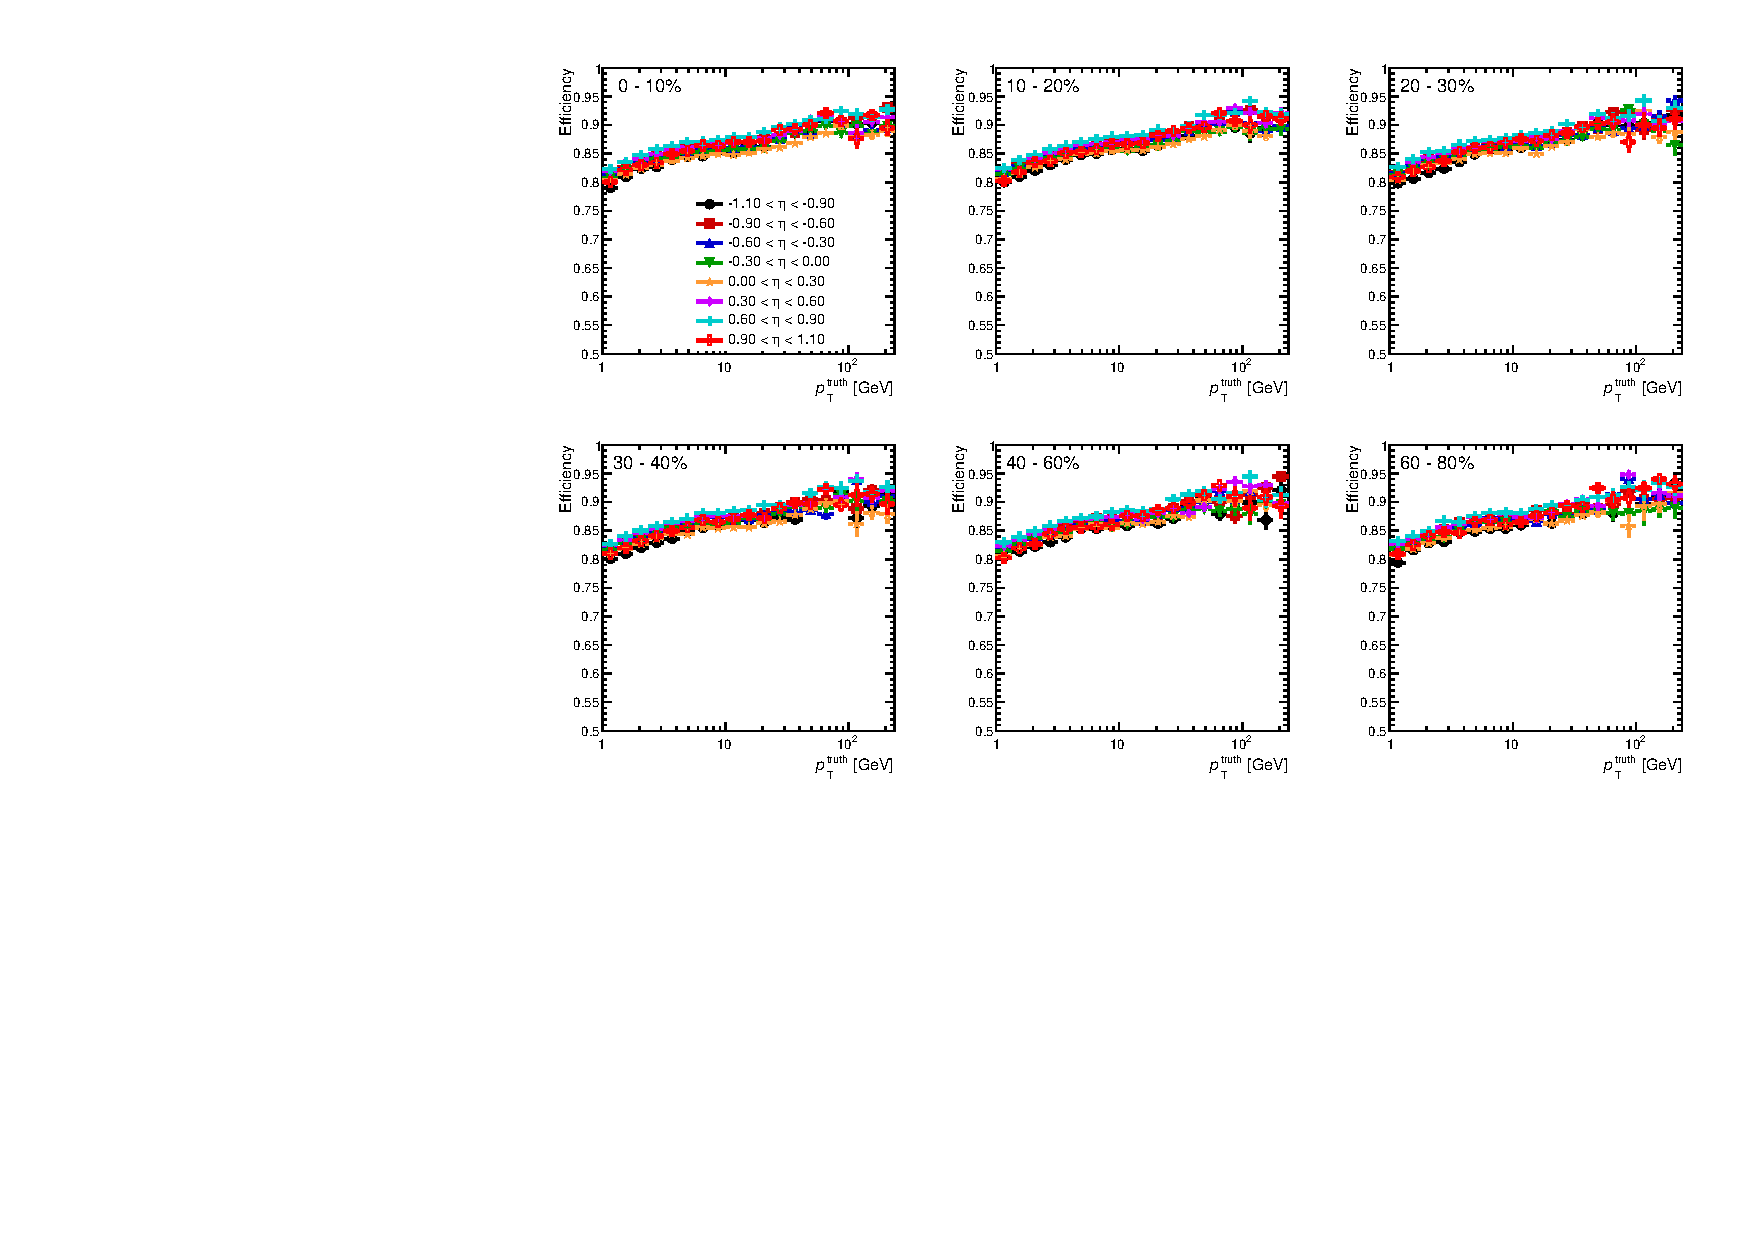
\includegraphics[width=0.9\textwidth]{figures_corrections/eff_cent_trketa_PbPb_ppTight.pdf}
   }
   \caption{Efficiency for reconstructing tracks evaluated using the default tracking selections in different track \eta\ bins in the data overlay \pbpb\ MC samples. Each panel is a different centrality bin..}
   \label{fig:pbpbeffdefault_final}
\end{figure}

\begin{figure}[ht]
   \centerline{
      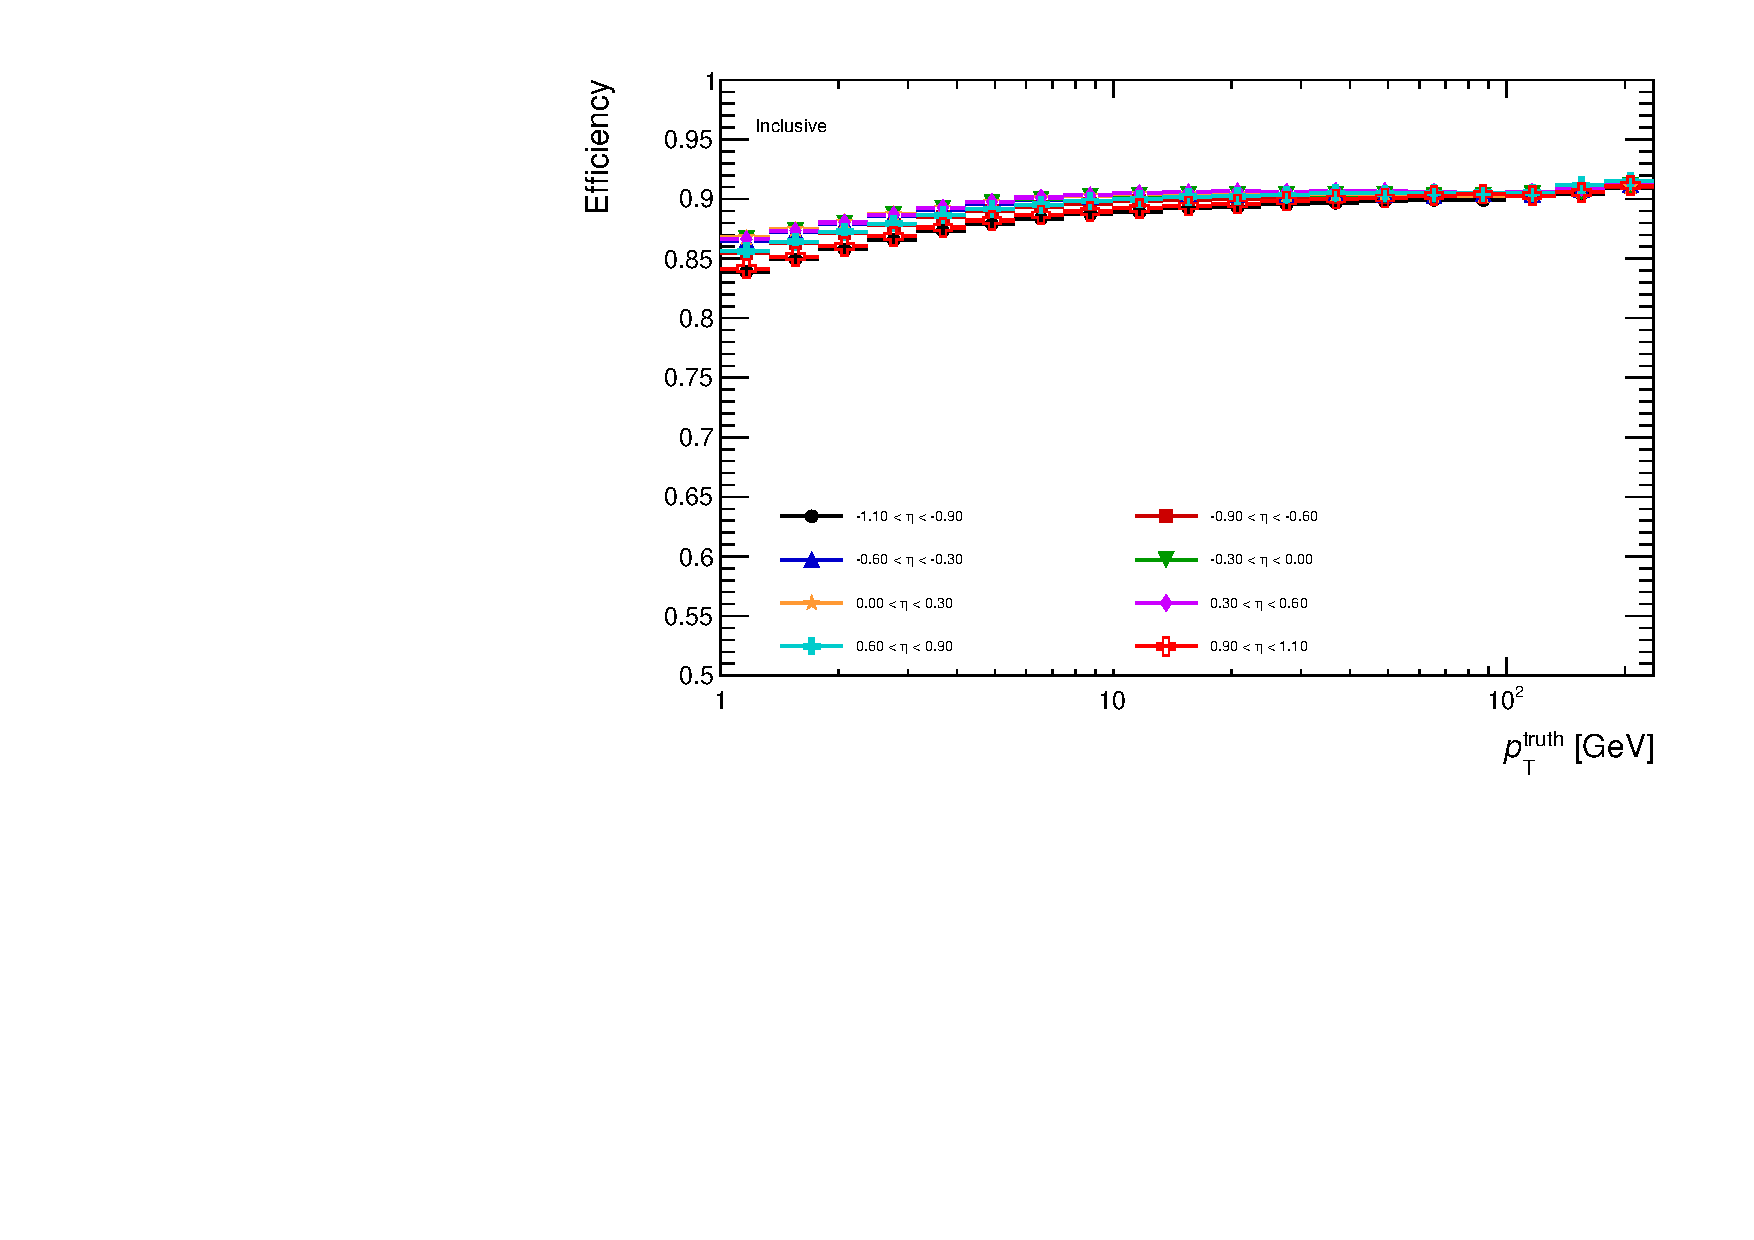
\includegraphics[width=0.55\textwidth]{figures_corrections/eff_cent_trketa_pp_ppTight.pdf}
   }
   \caption{Efficiency for reconstructing tracks evaluated using the default tracking selections in different track \eta\ bins in the \pp\ MC samples.}
   \label{fig:ppeffdefault_final}
\end{figure}

The final efficiency corrections applied were determined and applied as a function track \pt\ and track \eta, and can be seen in Figures~\ref{fig:pbpbeffdefault_final}-\ref{fig:ppeffdefault_final} for \pp\ and \PbPb\ collisions. No significant dependence on the collision centrality is observed. The efficiency exhibits a small, but monotonic increase with the track \pt. Only a small variation with the track $\eta$ is observed in the region $|\eta|<1.1$ The efficiency correction is applied on a track-by-track basis, assuming $\pttrk = \pTtrue$. While that assumption is not strictly valid, the efficiency varies sufficiently slowly with $\pTtrue$ that the error introduced by this assumption is negligible, up to 1\%. The tracking efficiency determined in Ref.~\cite{ATLAS502FFConf} was not seen to be dependent on \ptjet\ for $\pttrk \lesssim 40$ GeV as can be seen in Fig.~\ref{fig:pbpbeffdefaultjetpt_y0}-\ref{fig:ppeffdefaultjetpt}. The small depletion of the efficiency for tracks with $\pt \sim 10-40$~GeV was attributed to the convolution of how jet fragments and with the performance of the track reconstruction in the dense core of the jet~\cite{ATLAS502FFConf}. 


\begin{figure}[ht]
   \centerline{
      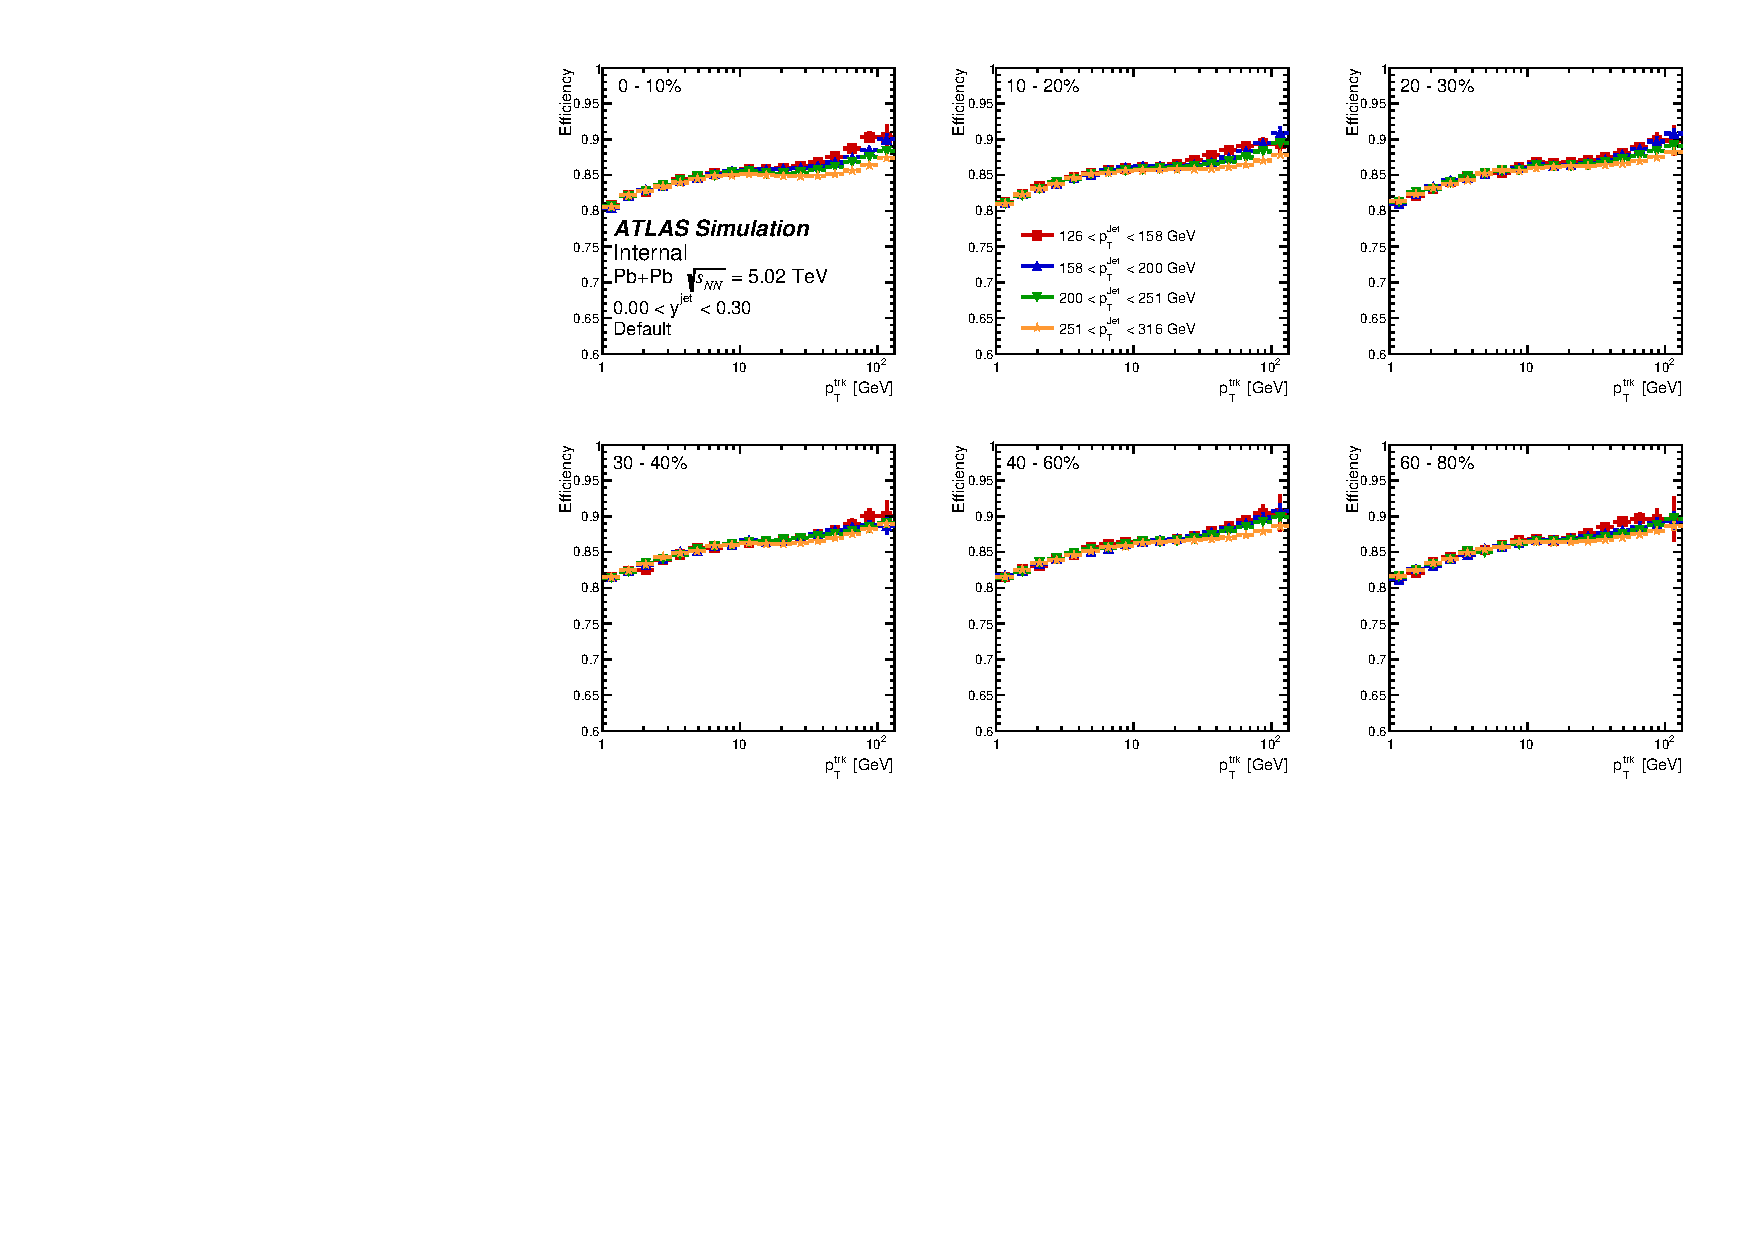
\includegraphics[width=0.9\textwidth]{figures_corrections/eff_centrality_jetpt_jety0_ppTight.pdf}
   }
   \caption{Efficiency for reconstructing tracks evaluated using the default tracking selections in different jet \pT\ bins and jet rapidity interval $|y|<0.3$ in the data overlay \pbpb\ MC samples. Each panel is a different centrality bin..}
   \label{fig:pbpbeffdefaultjetpt_y0}
\end{figure}

\begin{figure}[ht]
   \centerline{
      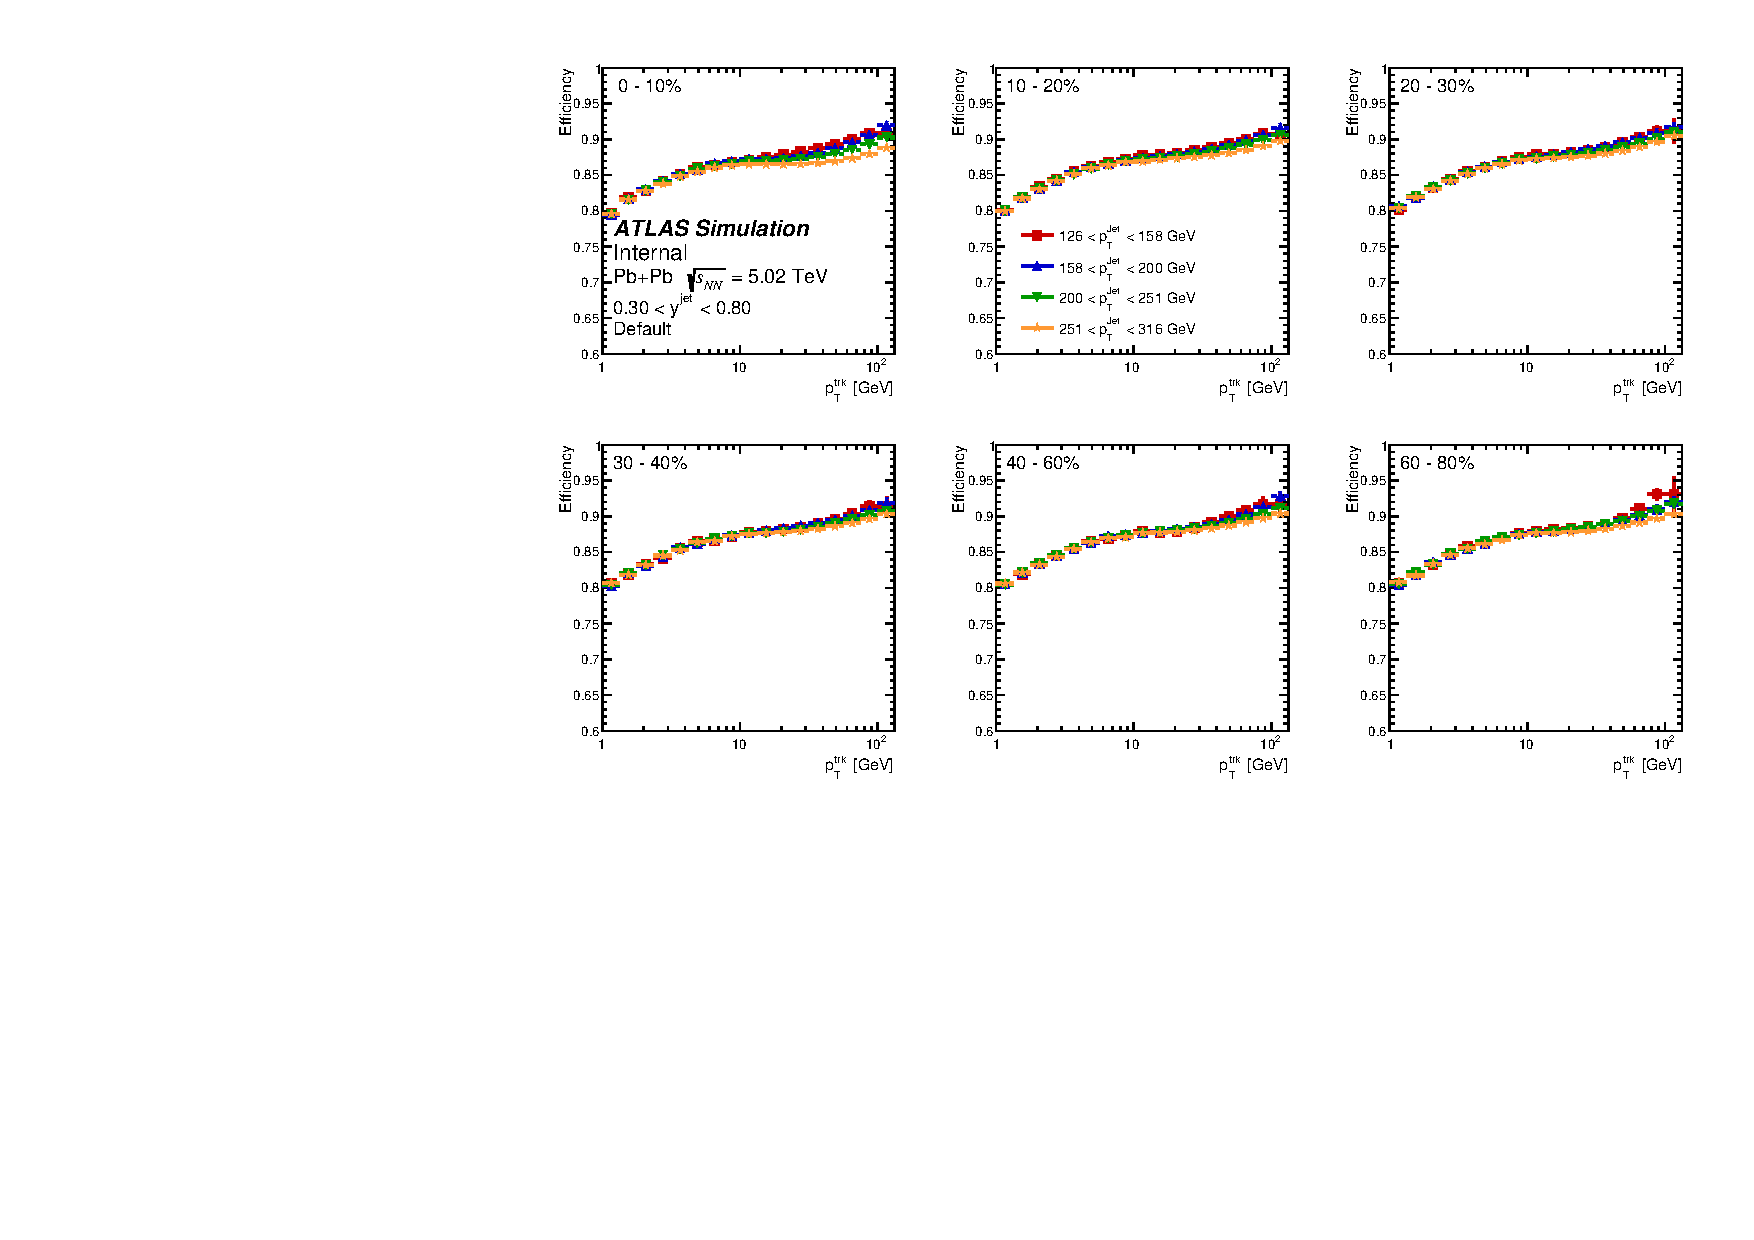
\includegraphics[width=0.9\textwidth]{figures_corrections/eff_centrality_jetpt_jety1_ppTight.pdf}
   }
   \caption{Efficiency for reconstructing tracks evaluated using the default tracking selections in different jet \pT\ bins and jet rapidity interval $0.3<|y|<0.8$ in the data overlay \pbpb\ MC samples. Each panel is a different centrality bin..}
   \label{fig:pbpbeffdefaultjetpt_y1}
\end{figure}

\begin{figure}[ht]
   \centerline{
      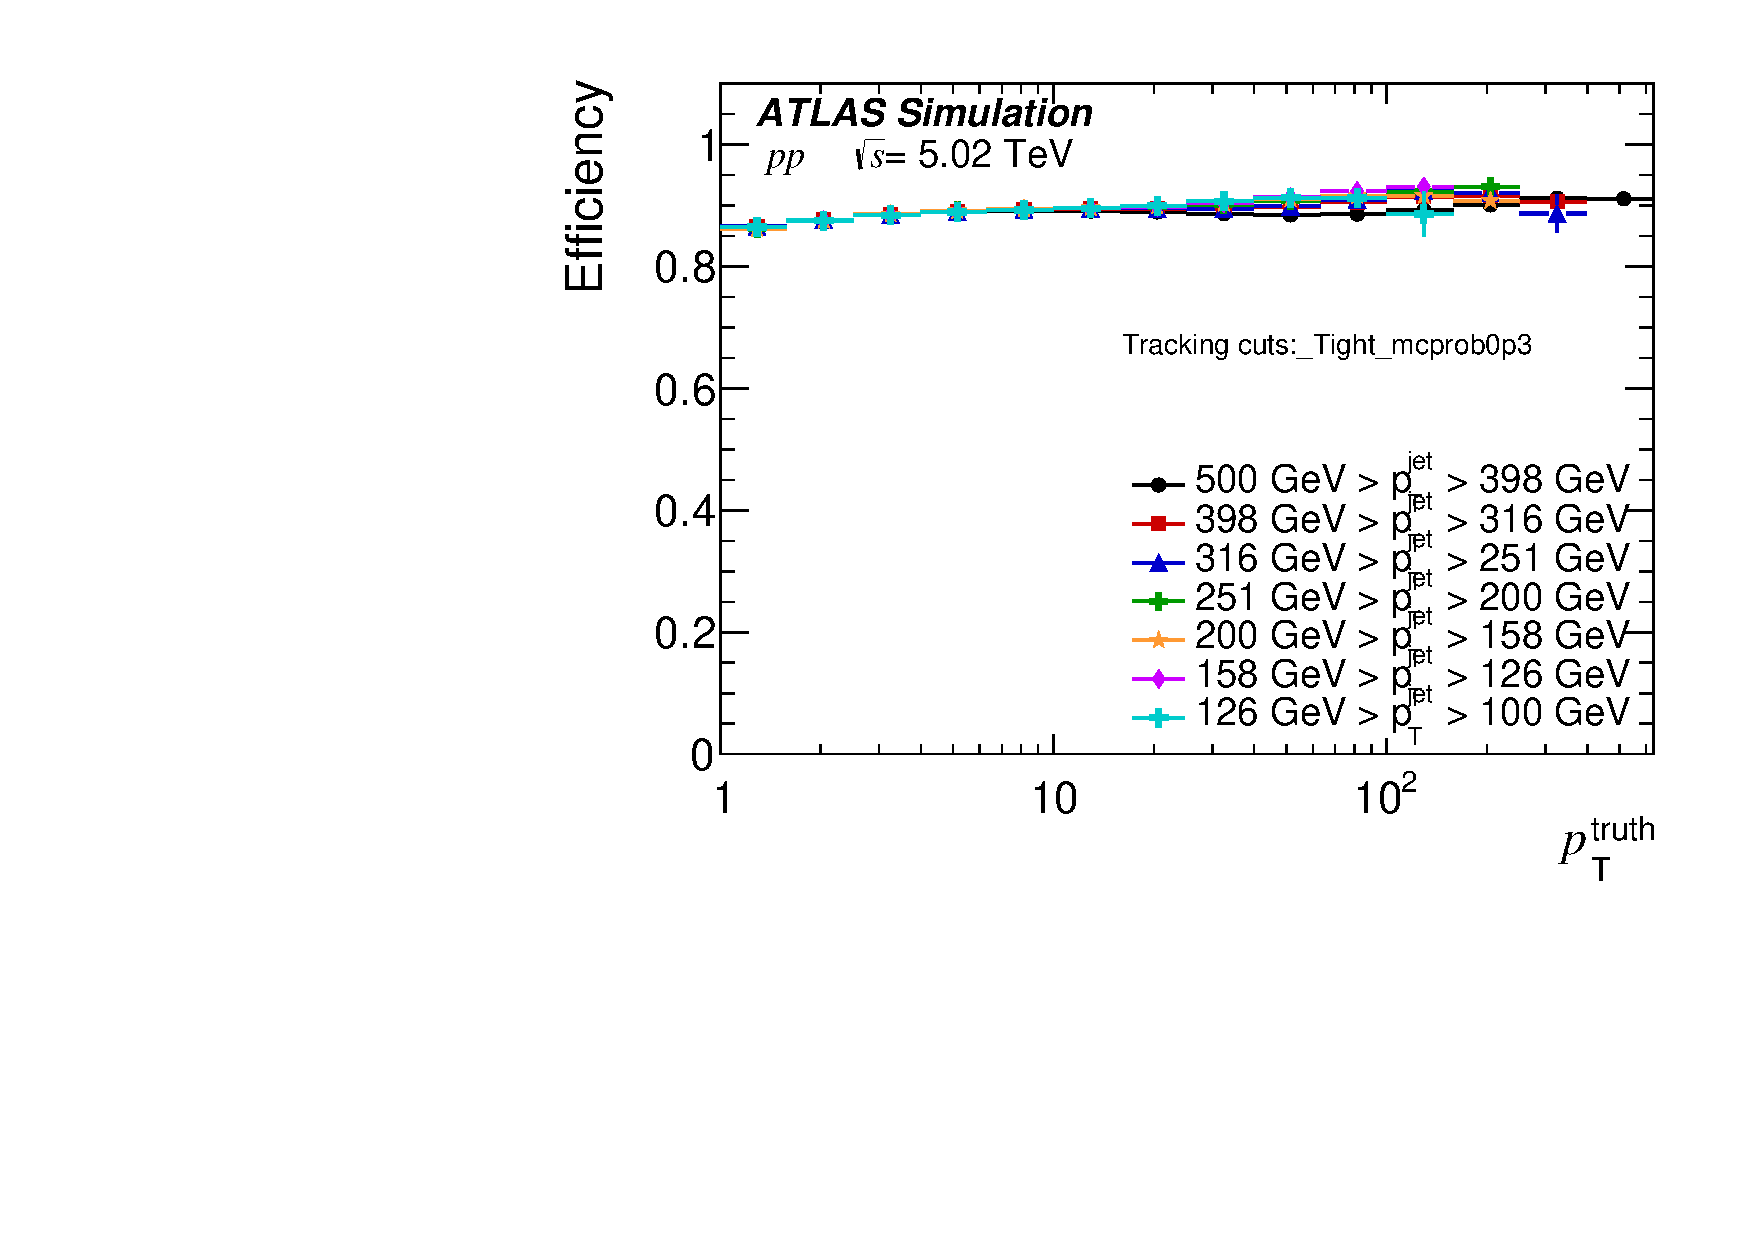
\includegraphics[width=0.55\textwidth]{figures_corrections/Trk_eff_v_pt_r005f_Tight_mcprob0p3_CX_Injet_0p0_0p3_pp_5p02.pdf}
   }
   \caption{Efficiency for reconstructing tracks evaluated using the default tracking selections in different jet \pT\ bins, in the \pp\ MC samples. }
   \label{fig:ppeffdefaultjetpt}
\end{figure}

\clearpage


\subsection{Fake rates}
\label{sec:fakerates}

The rate of fake tracks was evaluated and extensively studied in Ref.~\cite{ATLAS502FFConf} in the \pp, \pbpb\ HIJING MC, and in \pbpb\ MC+overlay samples. The MC overlay sample is used to crosscheck the fake rate at higher \pt, but is not used for any corrections. It was shown that as the \pttrk\ approaches the  \ptjet\ the fraction of fake tracks increases due to the steeply falling spectra of generator level tracks. Figures~\ref{fig:fakeratepp} and~\ref{fig:fakeratepbpb} show the fraction of tracks that are identified as fakes, secondaries, or part of UE in case of \PbPb\ collisions as a function of \pttrk\ for selections in \ptjet in
\pp\ and \pbpb\ collisions, respectively.  The rate 
decreases with \pttrk\ up to approximately 10~GeV and then remains constant until \pttrk\ approaches \ptjet\
where the rate increases again.  In \pbpb\ collisions, the ``fake'' rate also includes tracks which are from the underlying event from the real collisions into which the jet is overlaid.  The rate of these underlying event tracks increases with decreasing \pttrk\ and increasing collision centrality. The contribution from UE is negligible for tracks with \pT\ above 10 GeV as no centrality dependence is seen. The Fig.~\ref{fig:fakeratepbpb} excludes the very low \pT\ region where the distribution would be completely dominated by the UE. The size of the UE is then presented further in Fig.~\ref{fig:UEimpact_r2}-\ref{fig:UEimpact_r6}. To separate the contribution of UE tracks (see section~\ref{sec:cuts_UE}) from the fake tracks in \PbPb\ collisions and cross-check the centrality dependence of the fake rate, 0.2M MB \PbPb\ fully reconstructed HIJING MC~\cite{Wang:1991hta} events was used. The HIJING MC generator is capable of simulating global properties of HI collisions. The estimated fake rate of tracks associated with jets with $\pT>40$ GeV is at the level of 1\% and it exhibits similar behavior as observed in Fig.~\ref{fig:fakeratepbpb}. No significant dependence of the fake rate on the collision centrality was found~\cite{ATLAS502FFConf}.
  
  \begin{figure}[ht]
  \centerline{
  \begin{tabular}{cc}
  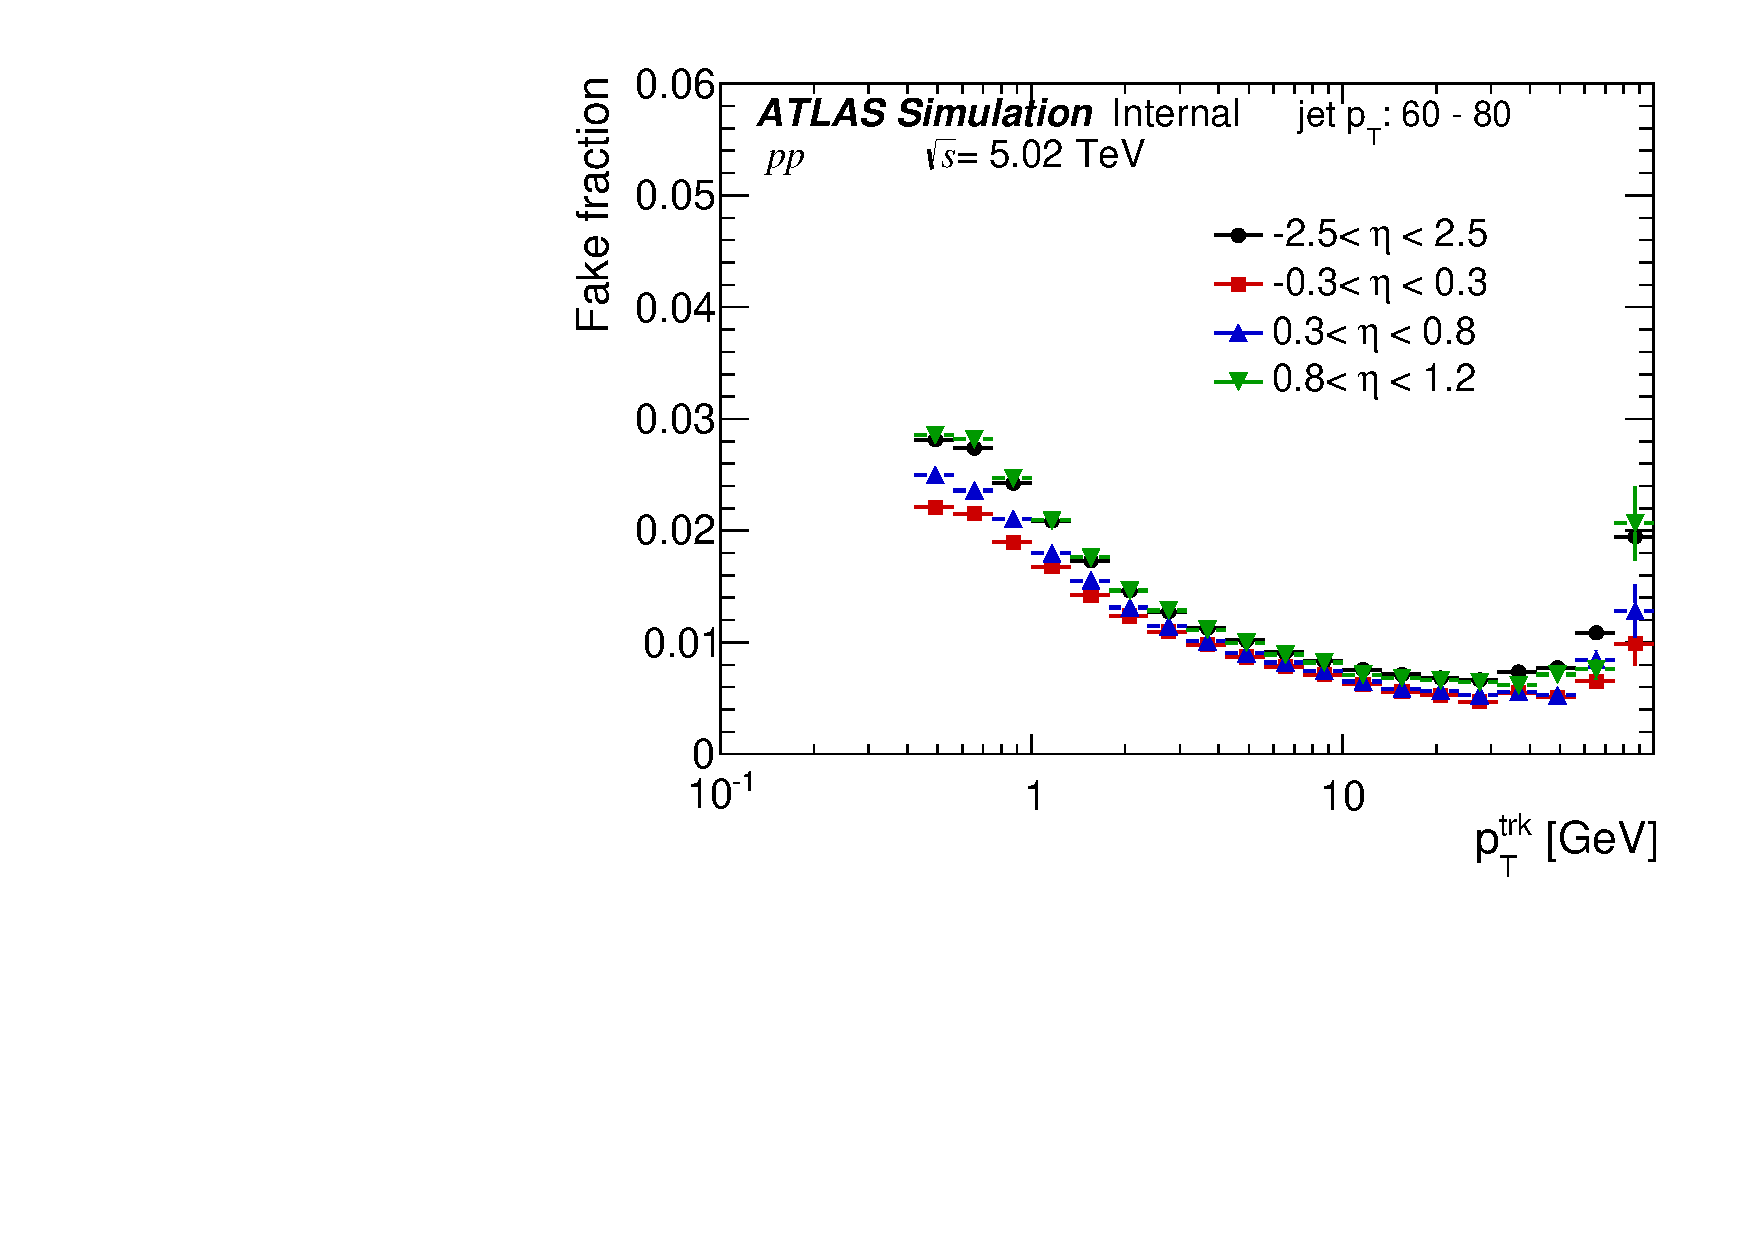
\includegraphics[width=0.45\textwidth]{figures_corrections/fake_rates/FakesEta_pp_5p02_r003_Tight_mcprob0p3_JZ2_jetpt_2.pdf} &
  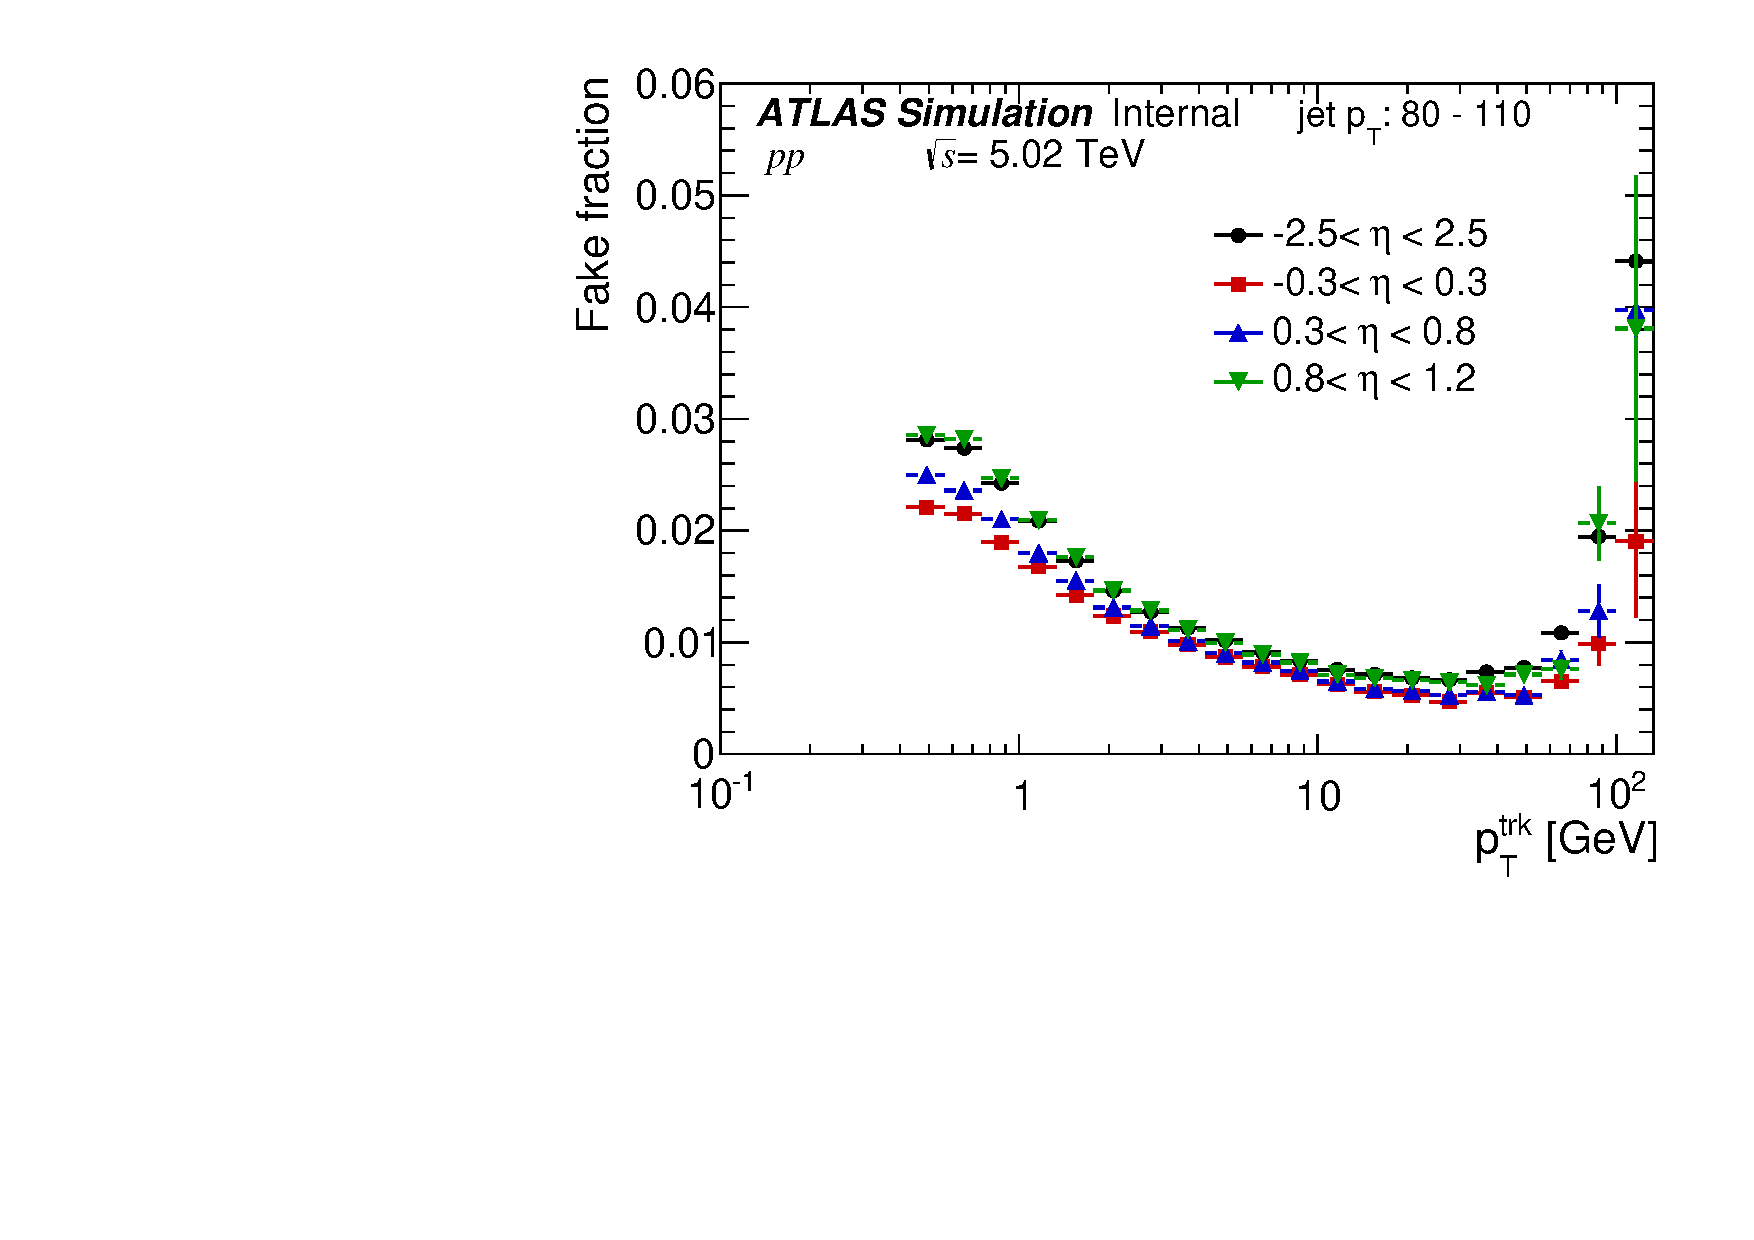
\includegraphics[width=0.45\textwidth]{figures_corrections/fake_rates/FakesEta_pp_5p02_r003_Tight_mcprob0p3_JZ2_jetpt_3.pdf} \\
    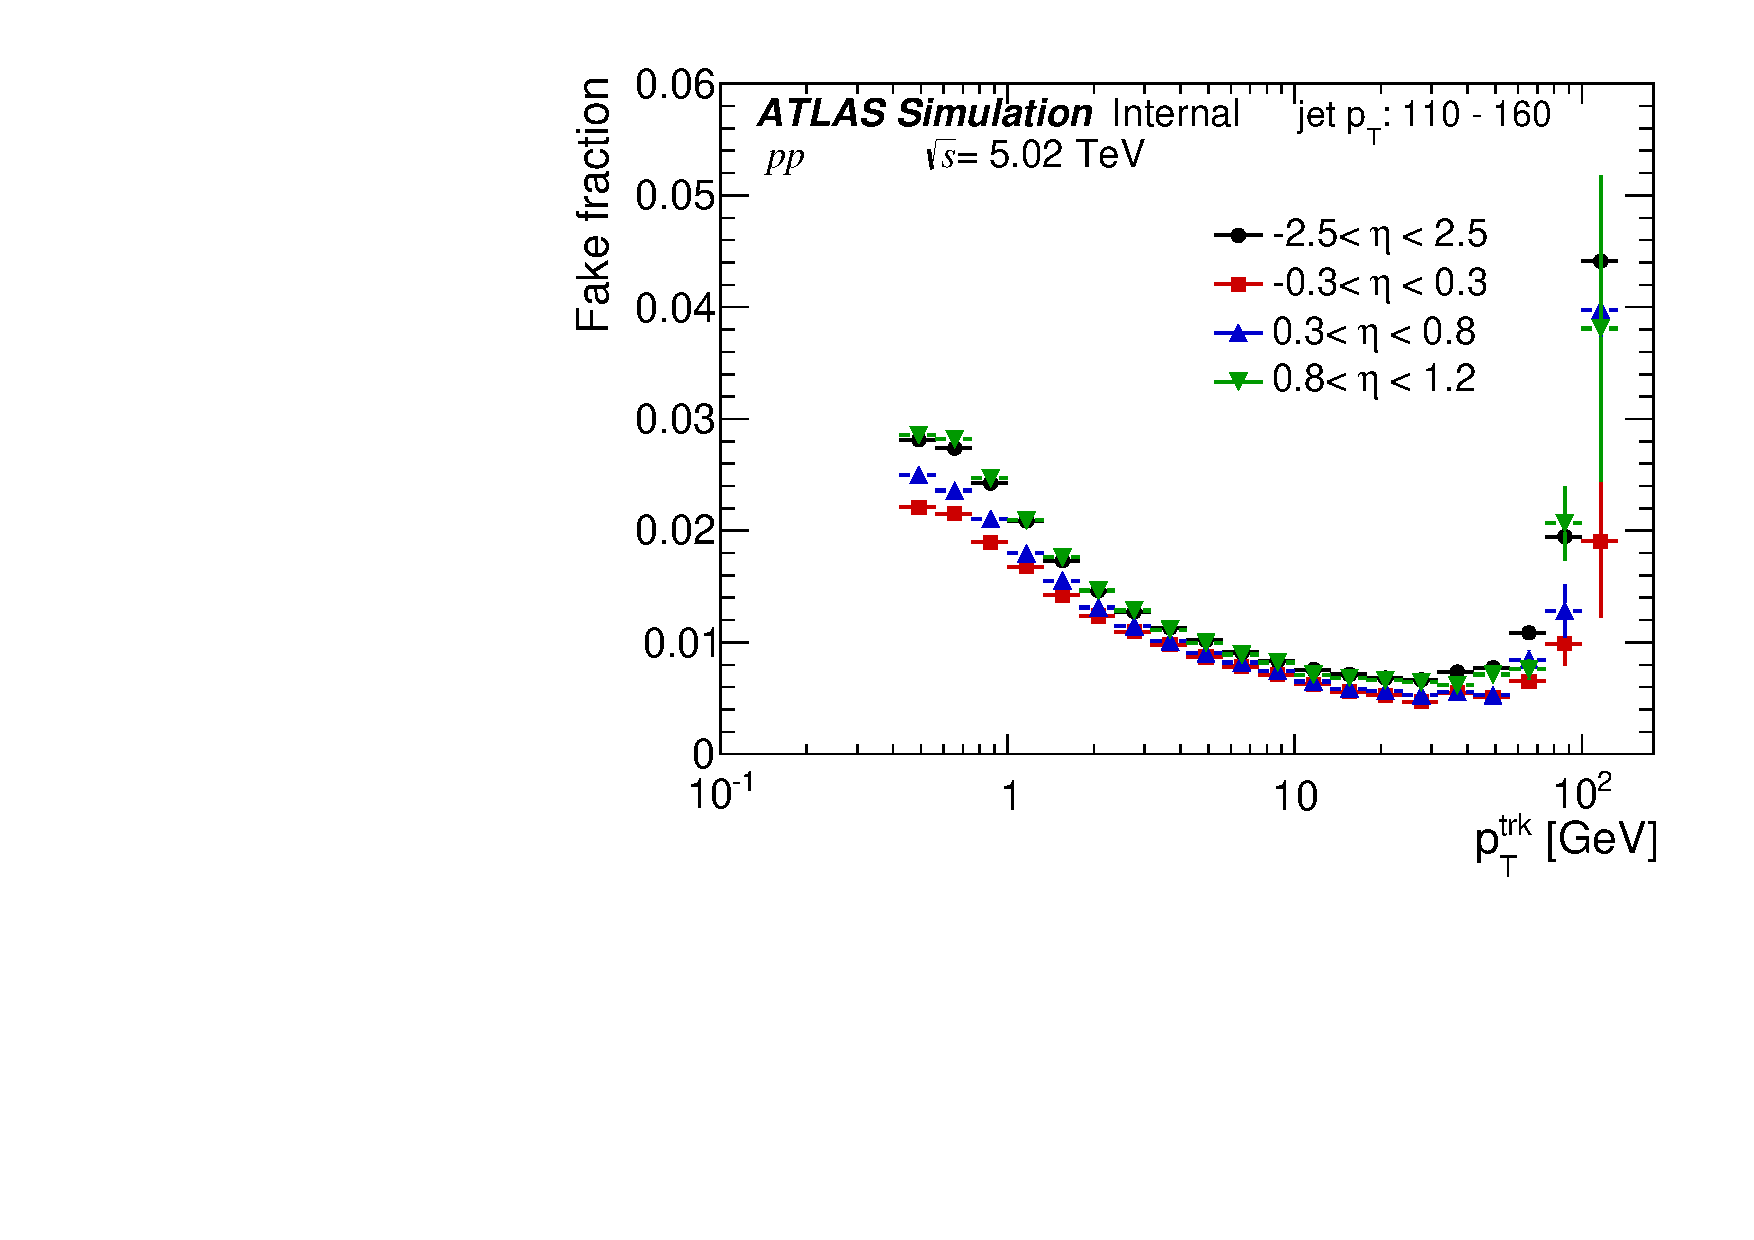
\includegraphics[width=0.45\textwidth]{figures_corrections/fake_rates/FakesEta_pp_5p02_r003_Tight_mcprob0p3_JZ2_jetpt_4.pdf} &
    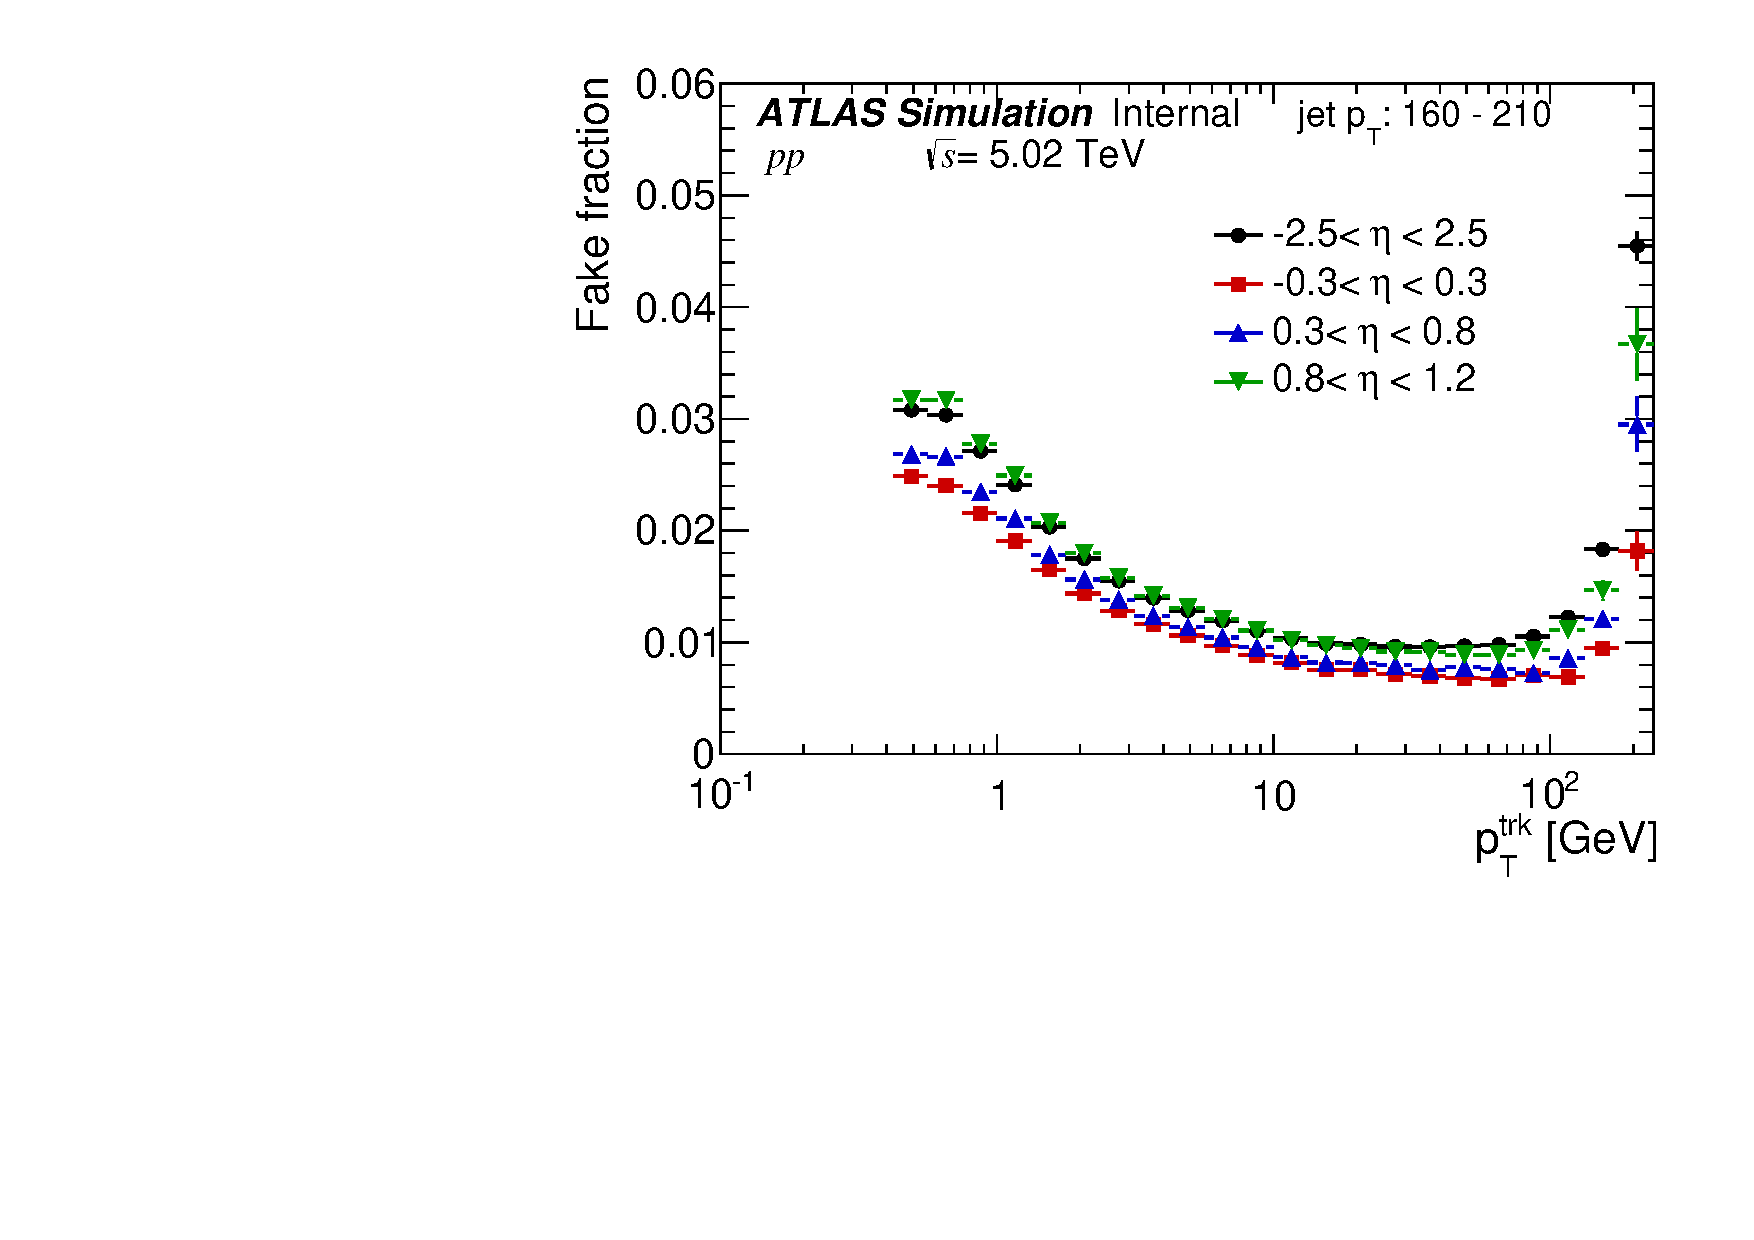
\includegraphics[width=0.45\textwidth]{figures_corrections/fake_rates/FakesEta_pp_5p02_r003_Tight_mcprob0p3_JZ3_jetpt_5.pdf} \\
      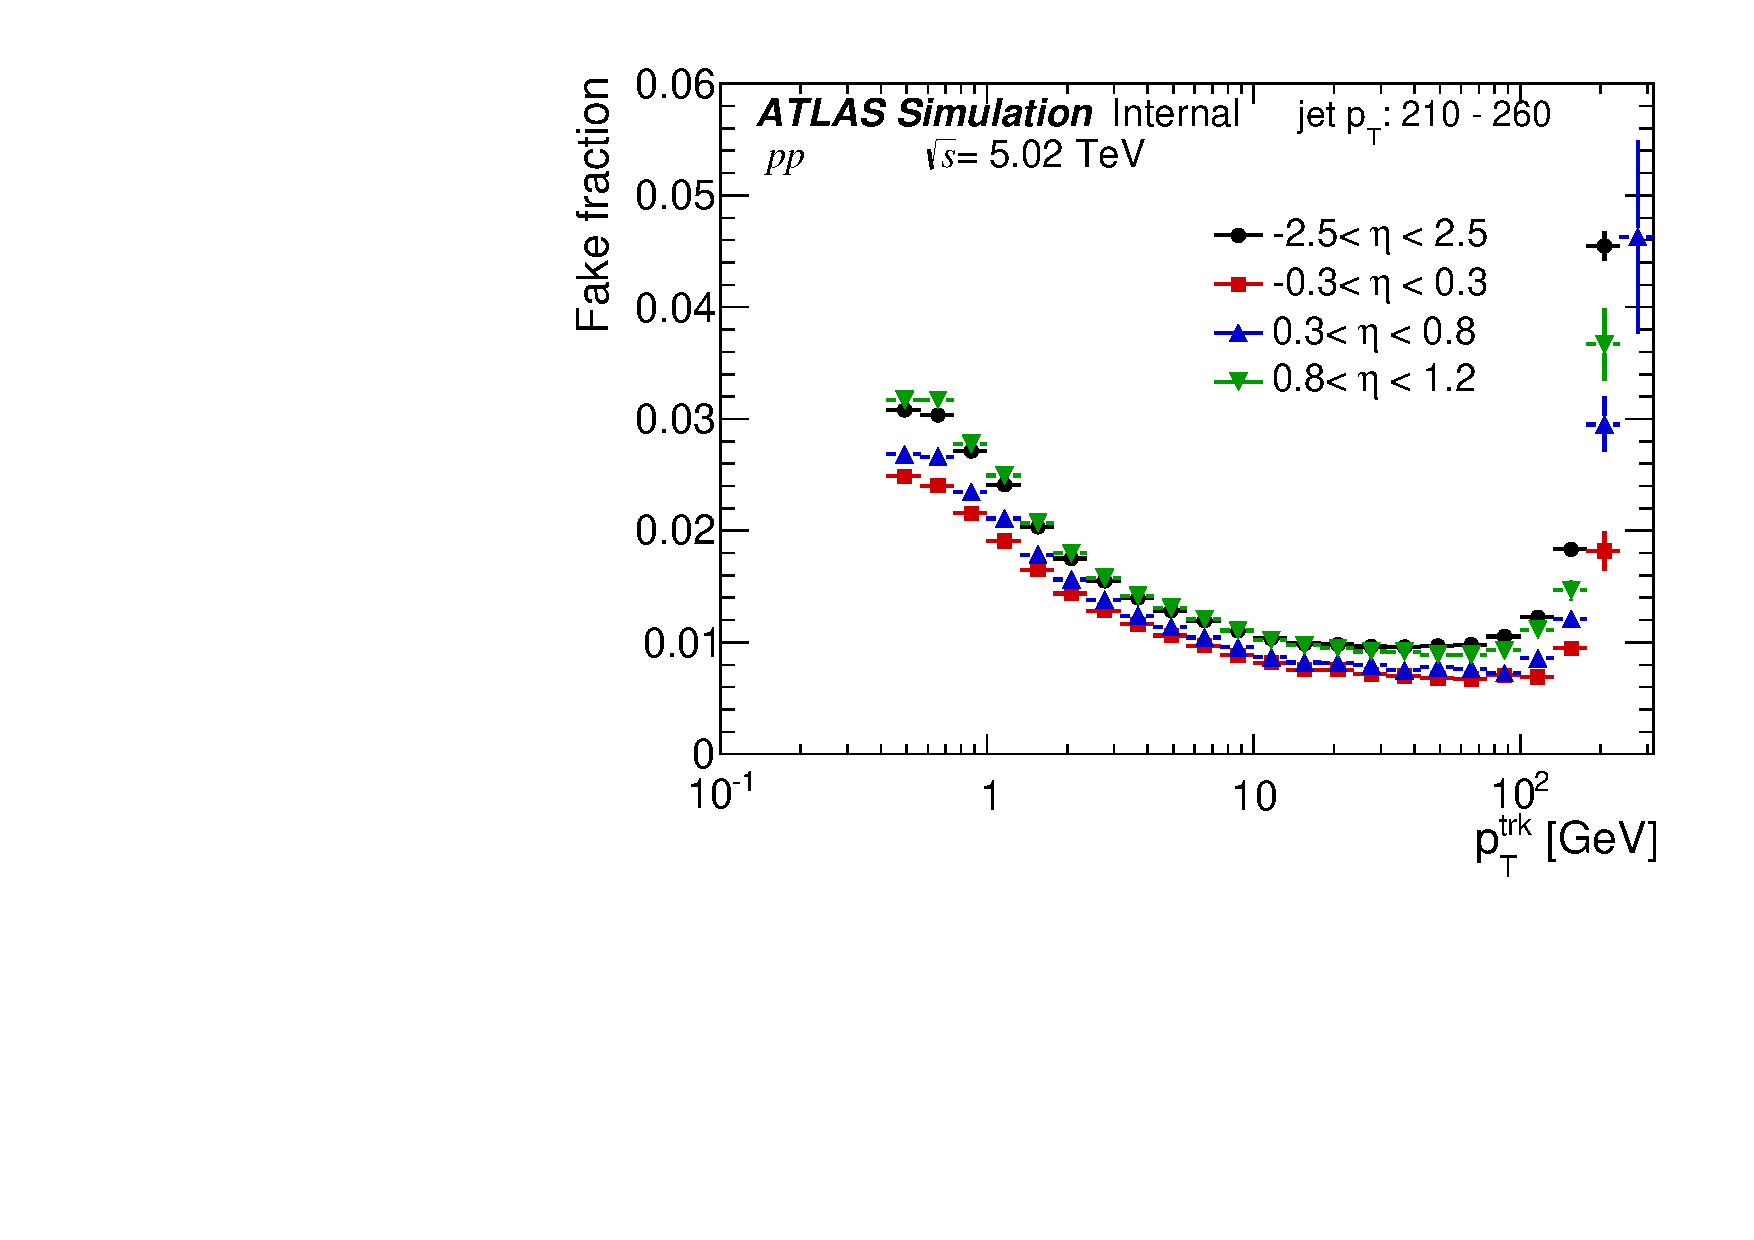
\includegraphics[width=0.45\textwidth]{figures_corrections/fake_rates/FakesEta_pp_5p02_r003_Tight_mcprob0p3_JZ3_jetpt_6.pdf} &
  \end{tabular}}
  \caption{Fake rate for five different \ptjet\ selections in 5.02 TeV \pp\ collisions and four pseudorapidity intervals. The fake rate is evaluated for default value of $MC_{\mathrm{prob}}$ cut of 0.3 used in 2015 analysis.}
  \label{fig:fakeratepp}
  \end{figure}  

  \begin{figure}[ht]
     \centerline{
	\begin{tabular}{cc}
	   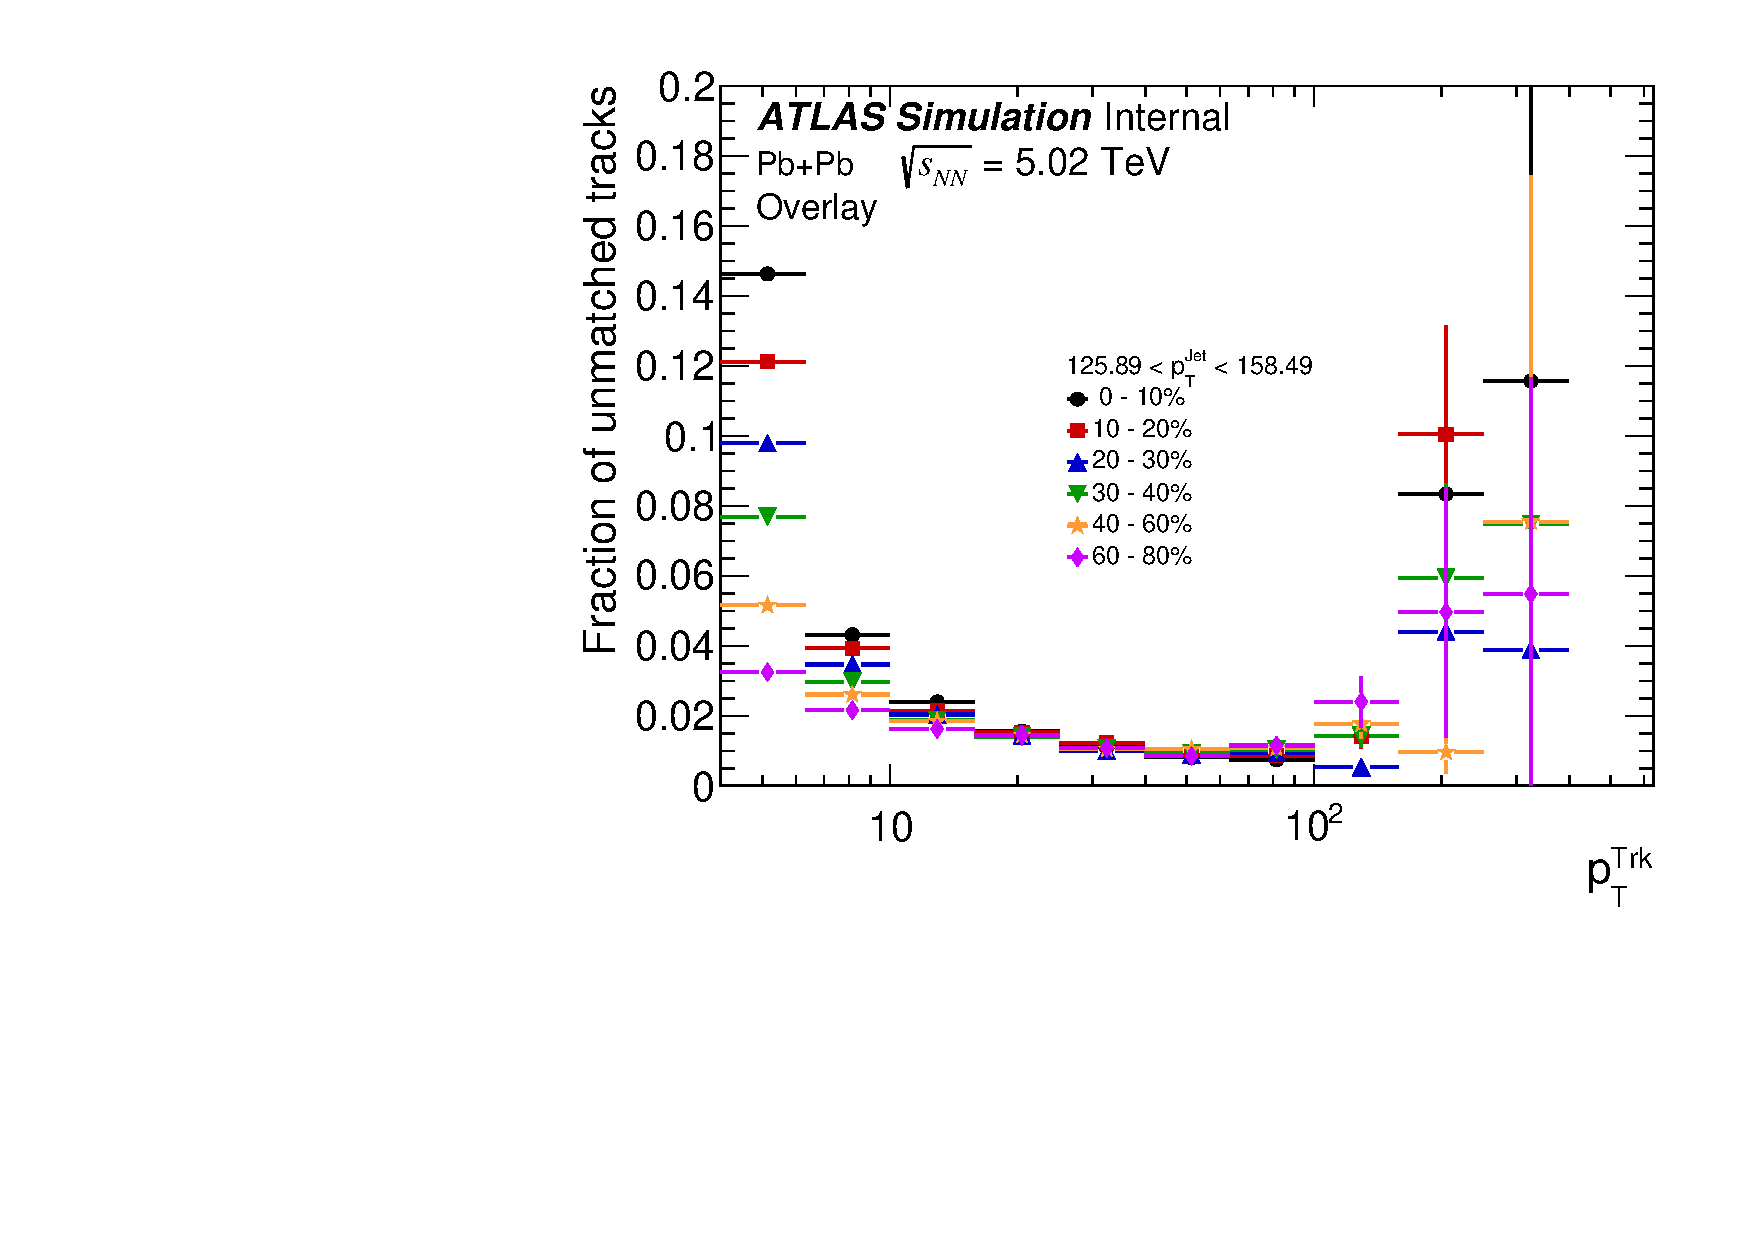
\includegraphics[width=0.45\textwidth]{figures_corrections/fake_rate_pt_125GeV.pdf} &
	   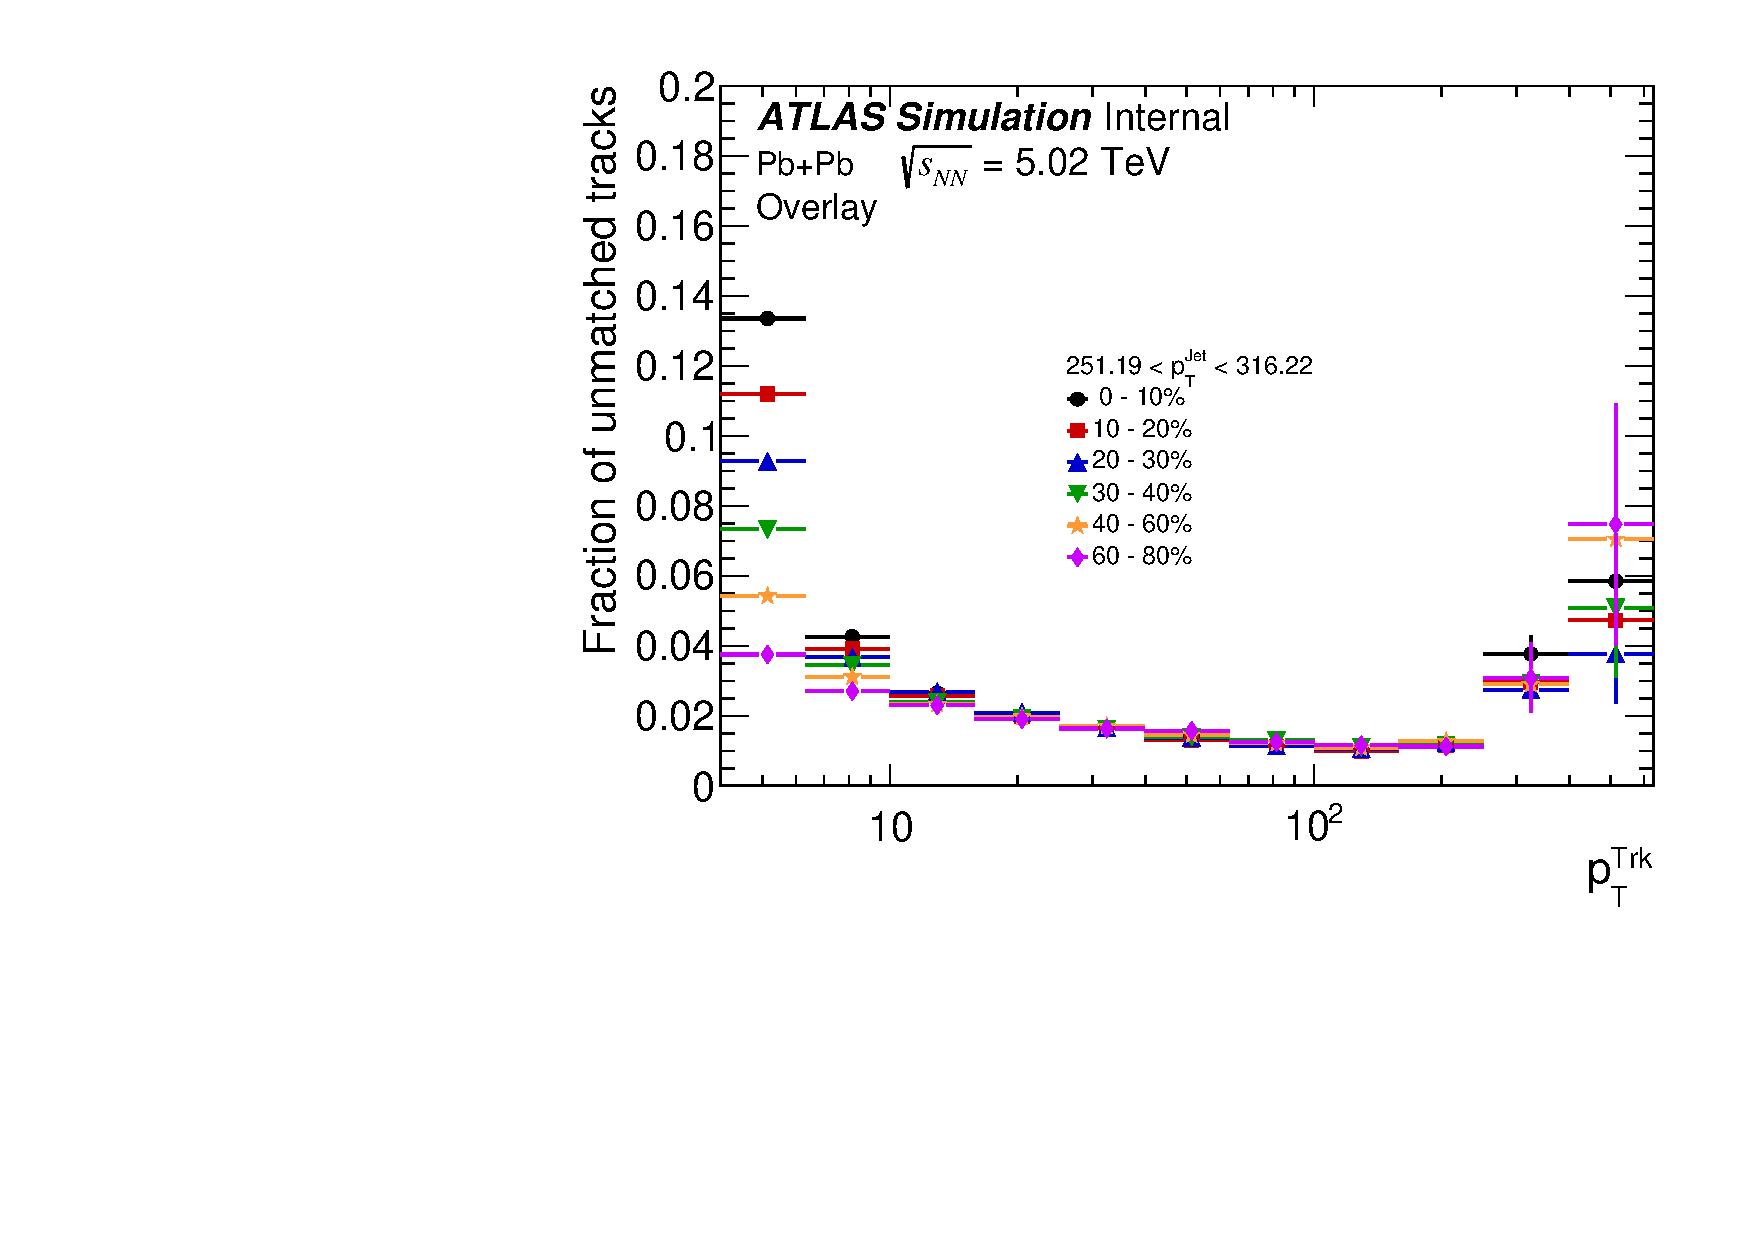
\includegraphics[width=0.45\textwidth]{figures_corrections/fake_rate_pt_251GeV.pdf} \\
	\end{tabular}
     }
     \caption{ Rate of tracks unmatched to truth tracks
	in \pbpb\ collisions for different centrality selections as indicated on the plot as a function of \pttrk.  
	The unmatched tracks include both fake tracks and tracks from the underlying event.  The panels show
	two \ptjet\ selections: 126-158~GeV (left) and 251-316~GeV (right). The low \pT\ part is omitted as it is dominated by the contribution from the UE.}
     \label{fig:fakeratepbpb}
  \end{figure}

  \begin{figure}[ht]
  \centerline{
	   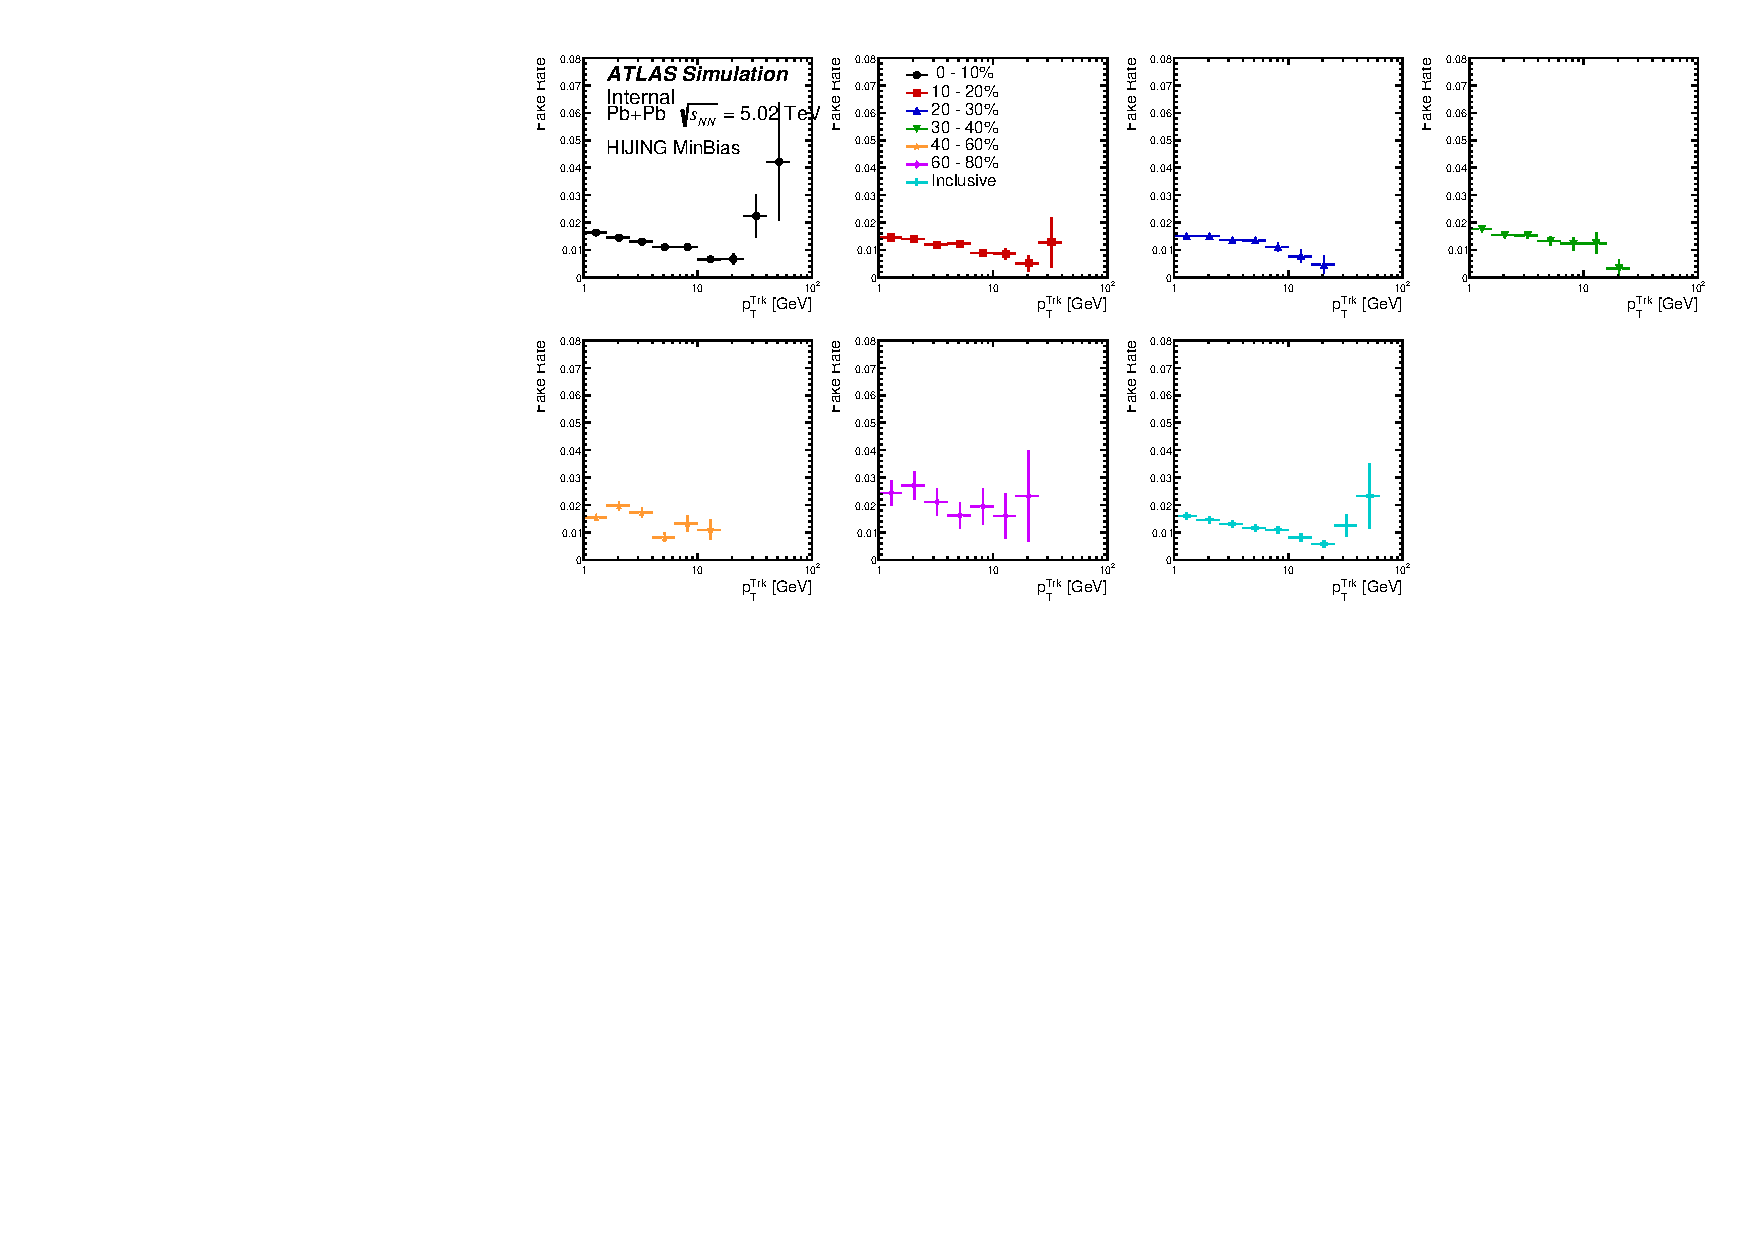
\includegraphics[width=1.\textwidth]{figures_performance/fake_rate_hijingMB.pdf}
	   }
     \caption{ Fake rate for six different centrality intervals in 5.02 TeV \pbpb\ HIJING MC collisions. The fake rate is evaluated for default value of $\mathrm{MC_{Probcut}}$ of 0.3 used in 2015 analysis. }
     \label{fig:fakeratehijing}
  \end{figure}



To correct for the contribution from fake and secondary particles, charged particle distributions are estimated using reconstructed tracks that do not have a truth match as defined by criteria described in previous paragraphs. These distributions are then subtracted from the measured distributions both in the data and MC. This procedure is applied for tracks above 10 GeV in \PbPb\ collisions and for tracks above 1 GeV in \pp\ collisions.  The correction also removes any residual UE above 10~GeV in case of \PbPb. The choice of the 10 GeV cut is based on the centrality dependence of the rate of truth-unmatched tracks in MC overlay samples shown in Fig.~\ref{fig:fakeratepbpb}. The correction for UE, fake and secondary tracks below 10 GeV in \PbPb\ collisions is discussed in the next section.

\clearpage

\subsection{Underlying event subtraction of tracks}
\label{sec:cuts_UE}

The underlying event subtraction performed on the calorimetric jet energy is described in Sec.~\ref{sec:reconstruction}. Charged particles from the nucleon-nucleon scatterings that are not associated with the hard scattering in question constitute a background to the \Dptr\ distributions that needs to be subtracted from the measured distributions. This background strongly depends on the collisions centrality and on the charged particle \pt. In the measurement of the inclusive jet fragmentation functions it was found that the UE contribution is negligible for charged particles with $\pt>10$~GeV~\cite{PbPb5TeVIntNote}. This can be seen in the centrality dependence of the combined rate of fake and underlying event charged particles shown in Fig.~\ref{fig:fakeratepbpb} where no significant centrality dependence is observed for track above 10 GeV. 

Two methods are used to estimate the underlying event for this analysis. The nominal ``Map method", and the alternative ``Cone method" to provide a systematic uncertainty. The former uses charged particle distributions of $\mathrm{d}N_{\mathrm{ch}}/\mathrm{d}\phi\mathrm{d}\eta(\mathrm{cent},\pt, \mathrm{d}\Psi_{\mathrm{ch}})$ in MC overlay events, while the latter evaluates the underlying event on an event-by-event basis using a grid of cones. 

\subsubsection{Map Method}
\label{sec:map_method}

%The UE contribution to a given annulus around the jet is estimated via $\mathrm{d}N_{\mathrm{ch}}/\mathrm{d}\phi\mathrm{d}\eta(\mathrm{cent},\pt, \mathrm{d}\Psi_{\mathrm{ch}})$ distributions of charged particles in MB overlay events.

In the "Map Method", $\eta-\phi$ maps of the average number of UE charged particles in a given annulus around a jet ($\nchUE^{\mathrm{Map}}$) are determined in MB overlay events using tracks without a truth match. The maps are filled as a function of the distance from the jet, \ptjet, \etajet, \phijet, angle of the jet to the reaction plane $ \mathrm{d}\Psi_{\mathrm{ch}}$, \pt\ and centrality.
%The reaction plane $\Psi$ is determined using the energy from the forward calorimeter. 
Examples of the these distributions for three different annuli (0--0.05, 0.25 -- 0.30, 0.60--0.70), in the $\mathrm{d}\Psi$ interval of  0.80 -- 1.00, for six collision centrality classes and for 1--1.6 GeV particles in 126 -- 158 GeV jets are shown in Fig.\ref{fig:ue_map}. The number of UE particles associated with a jet decreases with size of the annulus, decreasing centrality, increasing track \pT\ and increasing distance to the reaction plane. 
\begin{figure}[ht]
\centerline{
\begin{tabular}{ccc}
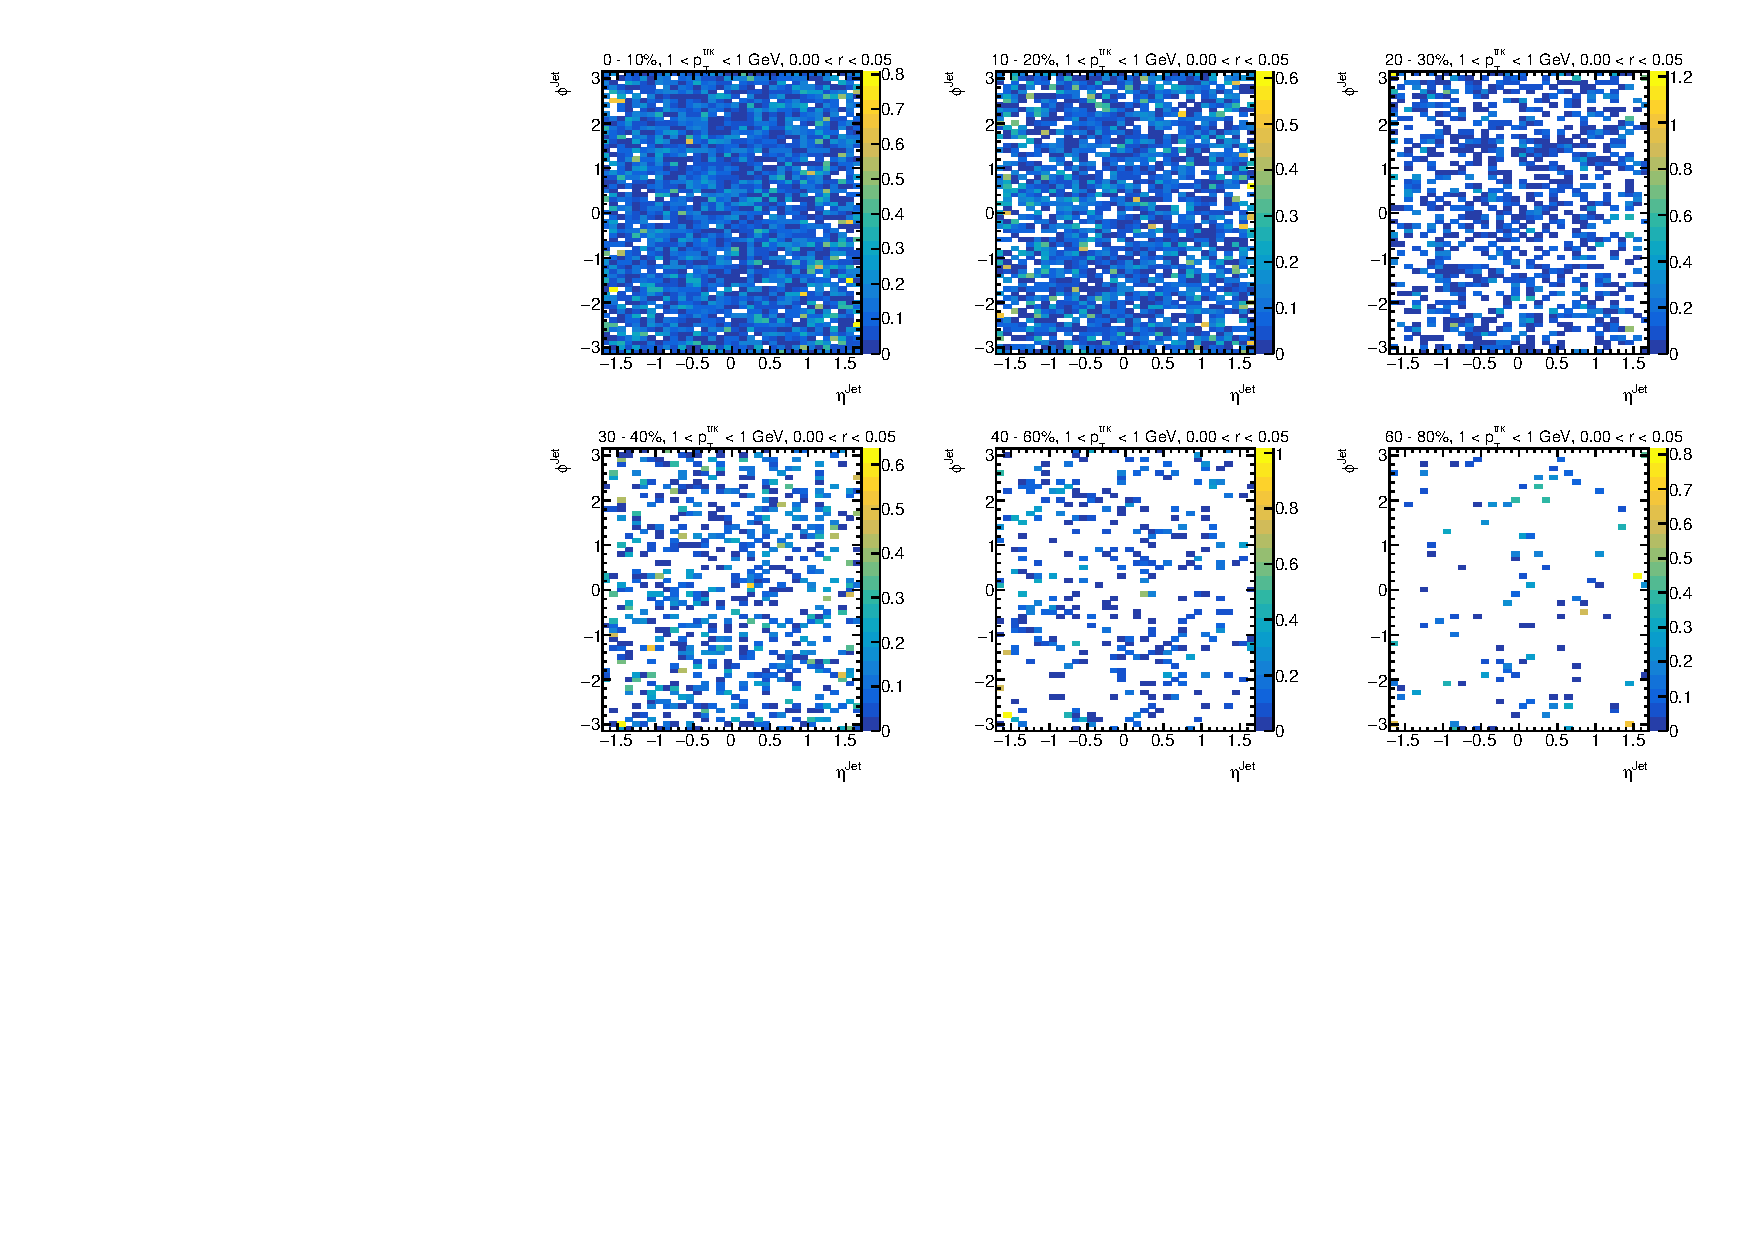
\includegraphics[width=0.7\textwidth]{figures_UE/eta_phi_map_trk2_dR0.pdf} \\
\includegraphics[width=0.7\textwidth]{figures_UE/eta_phi_map_trk2_dR5.pdf} \\
\includegraphics[width=0.7\textwidth]{figures_UE/eta_phi_map_trk2_dR9.pdf} \\
\end{tabular}}
\caption{
Per jet $\nchUE^{\mathrm{Map}}$ distributions of charged particles evaluated in the jet core, near the jet edge, and far from the jet, for  $\mathrm{d}\Psi$ in the interval 0.8--1.00 for six centralities, 1--1.6 GeV tracks, and 126--158 GeV jets.}
\label{fig:ue_map}
\end{figure}

The underlying event in MC is determined by applying the map method to MC. This is achieved by convoluting the $\nchUE^{\mathrm{Map}}$ distributions with the $\eta_{\mathrm{jet}}$, $\phi_{\mathrm{jet}}$, and $\mathrm{d}\Psi_{\mathrm{jet}}$ distributions of jets. The UE estimated by this method in MC consists of tracks without a truth match, and hence is the ``true'' underlying event by definition. This $\mathrm{UE}^{\mathrm{MC}}$ can then be used to correct any correlations between the underlying event as determined by the cone method and the JER (discussed in later sections). The UE normalized to unit area, as a function of $\Delta R$ with respect to the jet axis is shown in Fig.\ref{fig:UEdR} for the lowest track \pt\ interval where the UE contribution is the largest. The two distributions are the UE with and without secondary particles~\footnote{Secondary particles comes from weak decays of $\Lambda$, $K_{S}$, $\Xi$, $\Sigma$, $\Omega$ and from particles created in interactions with the material.}. The UE strongly decreases for more peripheral collisions and for increasing track \pt. Little radial dependence is seen when the secondaries are not included. A small effect is expected because there is an enhancement in the number of jets at mid rapidity, along with a decrease in the UE yield as a function of $\eta$. Since the secondaries are generated by primary PYTHIA particles, the enhancement is expected towards the jet core, where there is a higher multiplicity of primary particles.

The map method is then applied to data to measure the UE charged particle contribution to the measured \Dptr\ distributions. Since this method uses real MB \pbpb\ collisions (from the MC overlay samples), the underlying event distribution is that same as in the data. This method does not require a correction for the correlation between the underlying event and the JER because it is based on tracks without a truth match.
   
\begin{figure}[ht]
     \centerline{
        \includegraphics[width=0.9\textwidth]{figures_UE/UE_v_dR_pt1GeV.pdf}
     }
     \caption{UE estimated from tracks which do not have an associated truth particle in jet with \pt\ from 126 to 158 GeV and for the lowest track \pt\ interval (1--1.58 GeV). The two different distribution shows the UE with and without the contribution from the secondary particles.}
     \label{fig:UEdR}
  \end{figure}   

\subsubsection{Cone Method}
\label{sec:cone_method}
The cone method uses a regular grid of 9 cones of size $R = 0.8$ covering the full inner detector region (shown in Fig.\ref{fig:cone_grid}). The size of the cone corresponds to the radial phase space being investigated (0.8 in this case). Cones within a distance of $dR=1.6$ to a reconstructed jet are excluded if $\ptjet > 90$ GeV. They are also excluded if they contain a track with $\pt > 10$ GeV. The 10 GeV was cut was chosen based on the small centrality dependence of the combined rate of fake and underlying event tracks above 10 GeV as shown in Fig.\ref{fig:fakeratehijing}. The fraction of events as a function of number of cones used is shown in Fig.\ref{fig:cone_stats}. It can be seen that in MC the number of cones used is consistent with there being no jet quenching. Moreover, quenching in data leads to only one jet causing exclusions, consistent with most events using 7 cones.

\begin{figure}[ht]
     \centerline{
        \includegraphics[width=0.45\textwidth]{figures_UE/cone_grid.pdf}
     }
     \caption{Illustration of the cone method to estimate the underlying event. Cones numbered 3, 6, and 7 are excluded based based on the jet shown in red.}
     \label{fig:cone_grid}
  \end{figure}   

\begin{figure}[ht]
     \centerline{
        \includegraphics[width=0.45\textwidth]{figures_UE/cone_stats.pdf}
     }
     \caption{Fraction of events as a function of the number of cones used for the estimation of the underlying event.}
     \label{fig:cone_stats}
  \end{figure}   

The resulting UE charged particle yields $\fd \nchUE^{\mathrm{Cone}}/ \fd \pTch$ is evaluated over the 1 -- 10 GeV range as a function of \pt\, \ptjet\, centrality, and \rvar, and then averaged over all cones according to.

 \begin{eqnarray}
 \label{eq:Dptsub}
\frac{\fd n_{\mathrm{ch}}^{\mathrm{UE Cone}}}{\fd \pTch}  = \frac{1}{N_{\mathrm{cones}}} \frac{1}{\varepsilon} \frac{\Delta N^{\mathrm{cone}}_{\mathrm{ch}} (\pTch, \ptjet, \etajet)}{\Delta \pTch}
 \end{eqnarray}

Here $N_{\mathrm{cones}}$ is the number of background cones associated with a given jet with \ptjet. $\Delta N^{\mathrm{cone}}_{\mathrm{ch}}$ is the number of charged particles summed across all background cones associated to the jet in question. The cone method estimates the UE yields only from events containing jets included in the analysis, ensuring that the background automatically had the correct distribution of centralities within a given centrality bin. The UE contribution as measured using the cone method in data needs to be further corrected for three effects:
%\begin{itemize}
%\item
 \subparagraph{Correction for $\eta$-dependence: } To account for differences in the yields of UE particles at the position of the jet and at the position of the track for the random cone entering the UE estimate, the $\eta$ distribution of charged particles from MB overlay events is used to appropriately weigh the UE tracks. The correction is then the ratio of the value of the $\fd \nch / \fd\eta$ at the position of the jet and the track. The impact of the correction in 0-10\% \pbpb\ collisions is shown in Fig.\ref{fig:eta_corr}

\begin{figure}[ht]
\centerline{ \includegraphics[width=0.45\textwidth]{figures_UE/eta_correction.pdf} }
\caption{ Ratio of the $\NchUECone$ distributions with and without the correction for $\eta$ dependence in the most central 0-10\% \pbpb\ collisions, evaluated with a subset of the data (70k events).}
\label{fig:eta_corr}
\end{figure}


 \subparagraph{Correction for flow: }  Elliptic flow is the characteristic sinusoidal modulation of the yields of particles along the azimuth in heavy ion collisions. The maximum amplitude of the modulation determines the reaction plane, with more momenta being measured in plane than out of plane. Ref \cite{ATLAS-CONF-2016-105} provides a basic measurement of the magnitude of the elliptic flow, and its \pt\ dependence. The correction for this effect was based on a parametrization of the \pTch and centrality dependence of previously measured elliptic flow coefficients, $v_{2}$ \cite{ATLAS-CONF-2016-105}. The reaction plane angle $\Psi$ is estimated on an event-by-event basis by using the $\phi$ variation of transverse energy in the forward calorimeter. The correction factor is evaluated as a function of the distance of the jet from the reaction plane $\cos2(\phijet - \Psi)$. The correction is less (greater) than unity for jets in a direction perpendicular (parallel) to the reaction plane. Jets perpendicular (parallel) to the plane typically have a lower (higher) UE, and a cone at a random position in the ID is corrected down (up). The size of the correction is at the level of a few percent, and decreases with increasing track \pt, as is shown in Fig.\ref{fig:flow_corr}
 
 \begin{figure}[ht]
\centerline{ \includegraphics[width=0.45 \textwidth]{figures_UE/flow_correction.pdf} }
\caption{ Ratio of the $\NchUECone$ distributions with and without the correction for elliptic flow in the most central 0-10\% \pbpb\ collisions, evaluated with a subset of the data (70k events).}
\label{fig:flow_corr}
\end{figure}

\subparagraph{UE and JER correlation}
%Since the MC samples utilize the overlay procedure, where the real MB \PbPb\ collisions are used overlaid onto PYTHIA di-jets events, the UE distribution is the same as in data. 

%The UE distributions can alternatively be calculated in MC samples from tracks that do not have an associated truth particle, $\fd \nchUE^{\mathrm{TM}}/ \fd \pTch$. This allowed us to study the size of the UE as a function of $r$ with respect to the jet axis. The UE estimated using this method is also needed to correct for the correlation between UE and JER and the enhancement of the rate of secondary particles in the jet which will be described below. The UE distribution normalized to unit area plotted as a function of $r$ with respect to the jet axis is shown in Fig.~\ref{fig:UEdR} for the lowest track \pt\ interval where the contribution of the UE is the largest. The two distributions represent the UE with and without the secondary particles. The UE strongly decreases with decreasing number of binary nucleon-nucleon as the collision centrality decreases. Only a very small dependence on the $r$ is seen for the UE when the secondary particles are not included. A small effect is expected as result of the pseudorapidity distribution of jets is enhanced towards the mid-rapidity region and the yields of UE particles decreases as a function of $\eta$, i.e. towards large $\Delta R$. As the secondary particles are generated by primary PYTHIA particles it is expected to see the enhancement towards the core of the jet when the multiplicity of primary particles is increased.      
  

The interplay between the UE and the JER will be described here is discussed in detail in Ref.~\cite{ATLAS-COM-PHYS-2012-1653}. Due to the steeply falling nature of the jet \pt\ spectra, the smearing due to jet energy resolution leads to a net migration of jets from lower \pt\ to higher \pt\ values (hereafter referred to as ``up-feeding'') such that a jet reconstructed with a given \pTrec\ will correspond, on average, to a lower truth jet \pT, \avgpttrue. The up-feeding was observed to induce in the MC a difference between the UE yields determined using the MB overlay events and the actual UE contribution to reconstructed jets. The magnitude of this difference was found to be centrality dependent and exhibited a weak \pTjet\ dependence.
That difference was found to result from intrinsic correlations between the UE contribution to the yield of particles measured inside the jet and the MC \pTjet\ shift, $\Delta p_{\mathrm{T}}^{\mathrm{jet}}= \pTrec - \pTtrue$.  In particular, jets with positive (negative) $\Delta p_{\mathrm{T}}^{\mathrm{jet}}$ were found to have an UE contribution larger (smaller) than jets with $\Delta p_{\mathrm{T}}^{\mathrm{jet}} \sim 0$.  
 
  To correct for this effect, the centrality-, $\pTjet$-, $r-$ and $\pTch$-dependent multiplicative correction factors were applied on $\fd \nchUE^{\mathrm{Cone}}/ \fd \pTch$ distributions. 
  These multiplicative factors, $w_{\mathrm{UE}}$, were estimated as a ratio of UE distributions calculated in MC samples using the "Map method", $\Dptr_{f}$, and the "Cone Method".
  \begin{eqnarray}
  w_{\mathrm{UE}} (\pT) = \frac{\fd \nchUE^{\mathrm{Map}}/ \fd \pTch}{\fd \nchUE^{\mathrm{Cone}}/ \fd \pTch}\bigg|_{\mathrm{MC}}
  \end{eqnarray}   
Examples of these factors are shown in Fig~\ref{fig:UEweights_r2}-\ref{fig:UEweights_r6}. The correction by construction corrects also for fakes and secondary contribution in the track \pT\ region 1-10~GeV in \PbPb\ collisions. These factors are also shown in Figure~\ref{fig:UEweights_r_jet0}, as a function of \rvar\ for different track \pt\ bins, for $126 < \ptjet\ < 158 \GeV$.  The size of these corrections integrated over $\rvar = 0.4$ is comparable to the UE-JER correction done in \cite{ATLAS502FFConf}.

A comparison between the cone method and the map method is shown in Fig.\ref{fig:conemethod_mapmethod}. The difference between the methods varies slowly with \ptjet\ and track \pT, with a small centrality dependence coming from fact that the underlying event strongly depends on the centrality.

\begin{figure}[ht]
\centerline{
\includegraphics[page=2,width=1.\textwidth]{figures_UE/UE_factors.pdf} \\
}
\caption{
The multiplicative correction factors that correct for the correlation between the UE and the JER, fake and secondary particles in different centrality classes and $ 0.05 < r < 0.10$.}
\label{fig:UEweights_r2}
\end{figure}

\begin{figure}[ht]
\centerline{
\includegraphics[page=6,width=1.\textwidth]{figures_UE/UE_factors.pdf} \\
}
\caption{
The multiplicative correction factors that correct for the correlation between the UE and the JER, fake and secondary particles in different centrality classes and $ 0.25 < r < 0.30$.}
\label{fig:UEweights_r6}
\end{figure}

\begin{figure}
\centerline{\includegraphics[page=2,width=1.\textwidth]{figures_UE/UE_x_ratio}}
    \caption{The difference between the cone method and the map method as a function for \rvar\ for 0-10\% \pbpb\ collisions, in 126-158 GeV jets, 1-1.6 GeV tracks.}
    \label{fig:conemethod_mapmethod}
\end{figure}




\begin{figure}[ht]
\centerline{
\includegraphics[page=1,width=1.\textwidth]{figures_UE/UE_factors_r.pdf} \\
}
\caption{
The multiplicative correction factors that correct for the correlation between the UE and the JER, fake and secondary particles in different centrality classes, as a function of $r$ for $126 < \ptjet < 158 \GeV$.}
\label{fig:UEweights_r_jet0}
\end{figure}


Outside that region and in \pp\ system fake contribution is corrected as described at the beginning of Section~\ref{sec:trackreco}.  The corrected UE distributions, $\fd \cnchUE / \fd \pTch$ are then subtracted from measured distributions as follows
 %
 \begin{eqnarray}
 \label{eq:Dptsub}
\frac{\fd n_{\mathrm{ch}}^{\mathrm{sub}}}{\fd \pTch}  = \frac{\fd n_{\mathrm{ch}}^{\mathrm{meas}}}{\fd \pTch} - {w_{\mathrm{UE}} (\pT)} \left( \frac{\fd \nchUE^{\mathrm{Cone}}}{\fd \pTch} \bigg|_{\mathrm{Data}} \right)  = \frac{\fd n_{\mathrm{ch}}^{\mathrm{meas}}}{\fd \pTch} - \frac{\fd \cnchUE}{\fd \pTch}
 \end{eqnarray}

%The size of the $w_{\mathrm{UE}}$ correction is less than 1\% in kinematic regions where the UE is the largest, i.e. for low \pT\ charged particles inside the jet and at large $r$ distances for all track \pt. 
The absolute magnitude of the correction increases towards the higher track \pt\ in the jet core where the UE is smaller. This behavior originates from 1) the intrinsic correlations between the UE contribution to the yield of particles measured inside the jet and the MC \pTjet\ shift as it was discussed earlier; 2) the correlation of production of secondary particles with the jet.  The production of secondary particles is associated with presence of primary particles. Thus, the production of secondary particles is enhanced in the jet due to the higher density of primary particles compared to the regions outside a jet. This is shown in Fig.~\ref{fig:UEdR} where the UE evaluated in term of particles without matching to truth particles in MC with and without the contribution from secondary particles is presented and where the yield of secondary particles is significant only at smaller $dR$, i.e. within a jet.  Fig.~\ref{fig:UEdR} also shows that the relative yield of secondary particles to the yield of the UE particles is increasing with decreasing collisions centrality. Furthermore, the relative contribution of secondary particles to the UE increases with the track \pT\ as the fraction of the secondary particles decreases only slowly with the increasing track \pT\ (Figs.\ref{fig:fakeratepbpb}), however, the UE decreases strongly with the increasing track \pT\ (Fig.\ref{fig:UEimpact_r2}-\ref{fig:UEimpact_r6}). This results in lower UE contribution estimated using the MB collisions where tracks are not associated to a jet.

%The two methods give almost identical UE at angles outside the $R=0.4$ jet as the role of the two effect discussed here decreases.
     

The impact of the underlying event and fake track subtraction on the \Dptr\ distributions is shown in 
Figure~\ref{fig:UEimpact_r2}-\ref{fig:UEimpact_r6}.
The magnitude of this correction is the largest for low track \pt\ in central \pbpb\ collisions and the largest annulus. In the most extreme case the S/B ratios can be as low as 1/100.  The size of the correction decreases rapidly with increasing track \pt, decreasing centrality and towards the core of the jet.  In \pp\ collisions the magnitude of the fake track subtraction
is always much less than 5\%.

\begin{figure}[ht]
\centerline{
 \includegraphics[page=2,width=0.8\textwidth]{figures_UE/ChPS_B2S_PbPb_data.pdf} \\
}
 \caption{Ratio between the raw \Dptr\ distributions without and with the UE 
        subtraction in different centrality classes and different jet \pT\ intervals for $ 0.05 < r < 0.10$.}
    \label{fig:UEimpact_r2}
 \end{figure}

\begin{figure}[ht]
\centerline{
\includegraphics[page=6,width=0.8\textwidth]{figures_UE/ChPS_B2S_PbPb_data.pdf} \\
}
\caption{Ratio between the raw \Dptr\ distributions without and with the UE
subtraction in different centrality classes and different jet \pT\ intervals for $ 0.25 < r < 0.30$.}
\label{fig:UEimpact_r6}
\end{figure}


The basic performance of the UE subtraction has been tested in the MC overlay dataset. The closure test was performed using the MC overlay sample that has the same UE as in the data and will be discussed in the next subsection. The truth \Rdptr\ distributions were compared to fully corrected \Rdptr\ distributions where the  UE contribution is subtracted by the same method as used in the data (see Figure~\ref{fig:PbPb_ChPS_closure}). From the above mentioned tests we have concluded that the UE subtraction procedure is correct and works well. The UE estimate is subjected to variation as part of the systematic uncertainties. For the \pp\ data, we have not performed any UE subtraction.

\clearpage

\subsection{Unfolding}
\label{sec:unfolding}

Instrumental effects are corrected by an unfolding procedure. This analysis uses three separate unfolding procedures that are discussed in this section. 
\begin{itemize}

\item One dimensional unfolding for the \ptjet\ spectra for the normalization.
\item Two dimensional Bayesian unfolding in \pttrk\ and \ptjet for jet \pt\ dependent yields of charged particles.
\item Bin by bin correction for the jet and track position resolution.

\end{itemize}

 To achieve better correspondence with the data, the response matrices for both the one and two dimensional unfolding are reweighed so that the distributions match the shapes in the reconstructed data.
 
%The closure of the unfolding is checked by applying the response matrices from MC to the reconstructed spectra in MC.

\subsubsection{One Dimensional Unfolding for Jet Spectra}
\label{sec:1dunfolding}
The charged particle spectra need to be normalized by the number of jets in given jet \pt\ interval. Thus, the jet spectra needs to be corrected for bin migration due to the finite JER by unfolding procedure. 
%Since the primary effect to be unfolded for is the jet energy resolution (which is a much larger effect than the \pt\ resolution for charged tracks), one dimensional or bin-by-bin unfolding might seem to be appropriate. 
The unfolding is done via a one dimensional Bayesian unfolding procedure with 4 iterations implemented as part of the RooUnfold~\cite{Adye:2011gm} package. The \pp\ and \PbPb\ MC samples are used to construct two dimensional response matrices in terms of \ptjettruth\ and \ptjetreco. These matrices can be seen in Fig:\ref{fig:PbPb_jetspect_respmatrix}-\ref{fig:pp_jetspect_respmatrix} and are evaluated separately for \pp\ and in different centrality intervals for \PbPb\ collisions. The performance of the unfolding was verified by closure test, where the MC sample was used to derive the responses matrices that were then used to unfold the reconstructed jet spectra. Such unfolded distributions are than compared to those evaluated using truth jets. The jet spectra and MC closure is shown in Fig:\ref{fig:PbPb_jetspect_closure}-\ref{fig:pp_jetspect_closure}, as a function of \ptjet\ for jets in the. $|y| < $ 1.3 region. A good recovery of the truth distribution is seen, the MC closure is well within 1\% for \pbpb\ and \pp\ MC samples.

\begin{figure}[ht]
\centering
\includegraphics[page=5, width=0.9\textwidth]{figures_corrections/resp_matrix_jet_PbPb_MC.pdf}
\caption{The response matrices in terms of \ptjetreco\ and \ptjettruth\ in the jet $|y| < $1.3 region, in data overlay \pbpb\ MC samples. Each panel is a different centrality bin.}
\label{fig:PbPb_jetspect_respmatrix}
\end{figure}

\begin{figure}[ht]
\centering
\includegraphics[page=5, width=0.55\textwidth]{figures_corrections/resp_matrix_jet_pp_MC.pdf}
\caption{The response matrices in terms of \ptjetreco\ and \ptjettruth\ in the jet $y < $1.3 region, in \pp\ MC samples.}
\label{fig:pp_jetspect_respmatrix}
\end{figure}

\begin{figure}[ht]
\centering
\includegraphics[page=5, width=0.9\textwidth]{figures_corrections/spect_closure_PbPb_MC.pdf}
\caption{The jet spectra and MC closure as a function of \ptjet\ in the jet $|y| < $1.3 region, in data overlay \pbpb\ MC samples. The closure is seen to be well within 1\%. Each panel is a different centrality bin.}
\label{fig:PbPb_jetspect_closure}
\end{figure}

\begin{figure}[ht]
\centering
\includegraphics[page=5, width=0.55\textwidth]{figures_corrections/spect_closure_pp_MC.pdf}
\caption{The jet spectra and MC closure as a function of \ptjet\ in the jet $|\eta| < $1.3 region, in \pp\ MC samples. The closure is seen to be well within 1\%.}
\label{fig:pp_jetspect_closure}
\end{figure}



\subsubsection{Two Dimensional Unfolding for Charged Particle Spectra}
\label{sec:2dunfolding}


Observed correlation between the jet response in the detector and the jet fragmentation necessitates a two dimensional unfolding~\cite{ATLAS502FFConf}. 
%The dependence of the jet response on the fragmentation pattern of a particular jet has been studied extensively in ATLAS.
For example, gluon jets, which have in general a softer fragmentation function, are observed to have a lower energy response than quark jets~\cite{Aad:2014bia}.  The Global Sequential Calibration to the \pp\ jet collections~\cite{ATLAS:2015oia}, reduces the fragmentation dependence to the JES, but these calibrations are not available for the HI jet collections used in this analysis.

We use the RooUnfold~\cite{Adye:2011gm} implementation of the two dimensional iterative Bayesian unfolding~\cite{D'Agostini:1994zf} with 4 iterations. The MC \pbpb\ and \pp\ samples are used to construct a 4-dimensional response matrix in \pttrktruth, \ptjettruth, \pttrkreco, and \ptjetreco, shown in Fig:\ref{fig:PbPb_ChPS_respmatrix}-\ref{fig:pp_ChPS_respmatrix}. The response matrix $A_{ijkl}$ describes the probability that event from the truth track \pt\  bin $j$ and truth jet \pT\ bin $l$ is found in reconstructed bin $i$,$k$:
\begin{equation}
\mu_{jl} = \sum_{i,k} A_{ijkl}x^{\text{truth}}_{jl}.
\end{equation} 


\begin{figure}[ht]
\centering
\includegraphics[page=5, width=1.0\textwidth]{figures_corrections/resp_matrix_ChPS_PbPb_MC.pdf}
\caption{The response matrices in terms of \ptjetreco, \ptjettruth, \pttrkreco, and \pttrktruth, for reconstructed track - reconstructed jet pairs, that have 0.20 $< r < $0.25, in data overlay \pbpb\ MC samples. Each panel is a different centrality bin.}
\label{fig:PbPb_ChPS_respmatrix}
\end{figure}

\begin{figure}[ht]
\centering
\includegraphics[page=5, width=1.0\textwidth]{figures_corrections/resp_matrix_ChPS_pp_MC.pdf}
\caption{The response matrix in terms of \ptjetreco, \ptjettruth, \pttrkreco, and \pttrktruth, for reconstructed track - reconstructed jet pairs, that have 0.20 $< r < $0.25, in \pp\ MC samples}
\label{fig:pp_ChPS_respmatrix}
\end{figure}


\subsubsection{Bin-by-bin correction for Angular resolution}
\label{sec:bbbcorrection}

There is an additional unfolding procedure applied in this analysis to correct for the jet and the track position resolution that results in the migration in angular distance $r$. The migration is dominated by the poor jet angular resolution (Fig.\ref{Fig:PerformancepbpbJPReta0p4}-\ref{Fig:PerformancepbpbJPRphi0p4}), since the track angular resolution (Fig.\ref{fig:PbPb_trk_eta_res}-\ref{fig:PbPb_trk_phi_res}) is very good.

\begin{figure}[ht]
\centering
\includegraphics[width=0.9\textwidth]{figures_corrections/trk_res_eta_ppTight.pdf}
\caption{The $\eta$ resolution of the tracker in different $\eta$ bins for data overlay \pbpb\ MC samples. The different curves are different centralities, and it can be seen that there is no centrality dependence.}
\label{fig:PbPb_trk_eta_res}
\end{figure}

\begin{figure}[ht]
\centering
\includegraphics[width=0.9\textwidth]{figures_corrections/trk_res_phi_ppTight.pdf}
\caption{The $\phi$ resolution of the tracker in different $\phi$ bins for data overlay \pbpb\ MC samples. The different curves are different centralities, and it can be seen that there is no centrality dependence.}
\label{fig:PbPb_trk_phi_res}
\end{figure}

The correction factors are derived using response matrices that correlate the reconstructed and truth angular distance $r$. These matrices are evaluated for different jet and track \pT\ in different centrality classes. Examples of the response matrices are shown in Fig~\ref{fig:PbPb_bbb_2d_response} and Fig.~\ref{fig:pp_bbb_2d_response} for \pbpb\ and \pp\ MC samples. The bin-by-bin correction procedure is applied to \Dptr\ distribution unfolded to the particle level in terms of track and jet \pT\ by the two unfoldings discussed above. Thus, the correction factors for angular resolution were derived using the the reconstructed jets and tracks where the reconstructed jet and track \pT\ is replaced by the corresponding truth \pT. The bin-by-bin factors are then estimated as ratio of projections from the response matrices on the truth and reconstructed axis. These correction factors are shown in Fig.~\ref{fig:pos_corr_factors_PbPb_c0} and Fig.~\ref{fig:pos_corr_factors_pp} for \pbpb\ and \pp\ collisions as a function of \rvar.

\begin{figure}[ht]
\centering
\includegraphics[page=1, width=0.9\textwidth]{figures_corrections/ShapeResponse2D_PbPb.pdf}
\caption{The response matrix for the bin by bin correction applied to the unfolded charged particle spectra. This accounts for the jet position resolution. Each panel is a different \pttrk\ bin, for $126 < \ptjet\ < 158$ GeV jets, in central collisions from data overlay \pbpb\ MC samples}
\label{fig:PbPb_bbb_2d_response}
\end{figure}

\begin{figure}[ht]
\centering
\includegraphics[page=1, width=0.9\textwidth]{figures_corrections/ShapeResponse2D_pp.pdf}
\caption{The response matrix for the bin by bin correction applied to the unfolded charged particle spectra. This accounts for the jet position resolution. Each panel is a different \pttrk\ bin, for $126 < \ptjet\ < 158$ GeV jets, from \pp\ MC samples}
\label{fig:pp_bbb_2d_response}
\end{figure}


\begin{figure}[ht]
\centering
\includegraphics[page=1, width=0.9\textwidth]{figures_corrections/RatioProj_PbPb}
\caption{The correction factors applied to the unfolded charged particle spectra, shown for the most central collisions, as a function of $r$, with each panel showing a different track \pt\ bin, and each curve showing a different \ptjet\ range. These factors correct for the jet position resolution in \pbpb\ collisions.}
\label{fig:pos_corr_factors_PbPb_c0}
\end{figure}

\begin{figure}[ht]
\centering
\includegraphics[page=1, width=0.9\textwidth]{figures_corrections/RatioProj_pp}
\caption{The correction factors applied to the unfolded charged particle spectra, as a function of $r$, with each panel showing a different track \pt\ bin, and each curve showing a different \ptjet\ range. These factors correct for the jet position resolution in \pp\ collisions..}
\label{fig:pos_corr_factors_pp}
\end{figure}


The \Dptr\ distributions at various stages of the analysis in \pp\ MC and data (Fig:\ref{fig:evol_pp}), and \pbpb\ MC and data (Fig:\ref{fig:evol_PbPb_MC}-\ref{fig:evol_PbPb_data}) are also shown.

\begin{figure}[ht]
   \centerline{
      \begin{tabular}{c}
	\includegraphics[page=5, width=0.5\textwidth]{figures_corrections/evol_pp_MC.pdf}
	\includegraphics[page=5, width=0.5\textwidth]{figures_corrections/evol_pp_data.pdf}
   \end{tabular}
   }
   \caption{The evolution of the \Dptr\ distributions for \pp\ MC (left) and data (right) as various corrections are applied. The spectra is shown for tracks with $0.05 < \Delta r < 0.10$ away from the jet axis, for $126 < \ptjet < 158$ GeV. The ratios showing the effect of the unfolding and bin by bin corrections (left and right), as well as the MC closure (left) are shown in the lower half of the panels. }
      \label{fig:evol_pp}
   \end{figure}


\begin{figure}[ht]
\centerline{
\includegraphics[page=5, width=0.85\textwidth]{figures_corrections/evol_PbPb_MC.pdf}
}
\caption{The evolution of the \Dptr\ distributions for \PbPb\ MC as various corrections are applied. The spectra is shown for tracks with $0.05 < \Delta r < 0.10$ away from the jet axis, for $126 < \ptjet < 158 $GeV. The ratios showing the effect of the subtraction, unfolding and bin by bin correction (left and right), as well as the MC closure (left) are shown in the lower half of the panels. The different panels are different centrality selections.}
\label{fig:evol_PbPb_MC}
\end{figure}

\begin{figure}[ht]
\centerline{
\includegraphics[page=5, width=0.85\textwidth]{figures_corrections/evol_PbPb_data.pdf}
}
\caption{The evolution of the \Dptr\ distributions for \PbPb\ data (bottom six panels) as various corrections are applied. The spectra is shown for tracks with $0.05 < \Delta r < 0.10$ away from the jet axis, for $126 < \ptjet < 158 $GeV. The ratios showing the effect of the subtraction, unfolding and bin by bin correction (left and right), as well as the MC closure (left) are shown in the lower half of the panels. The different panels are different centrality selections.}
\label{fig:evol_PbPb_data}
\end{figure}


The MC closure of the charged particle spectra as a function of \pt\ in \pp\ and data overlay \pbpb\ MC samples can be seen in Fig:\ref{fig:PbPb_ChPS_closure}-\ref{fig:pp_ChPS_closure}, and is well within 1\% for low \pt\ particles.

\begin{figure}[ht]
\centering
\includegraphics[page=5, width=1.0\textwidth]{figures_corrections/ChPS_final_PbPb_MC.pdf}
\caption{The charged particle spectra and MC closure as a function of \pttrk\ for different \ptjet\ bins, reconstructed track - reconstructed jet pairs, that have 0.20 $< r < $0.25, in data overlay \pbpb\ MC samples. Each panel is a different centrality bin. The closure is seen to be well within 1\%.}
\label{fig:PbPb_ChPS_closure}
\end{figure}

\begin{figure}[ht]
\centering
\includegraphics[page=5, width=0.55\textwidth]{figures_corrections/ChPS_final_pp_MC.pdf}
\caption{The charged particle spectra and MC closure as a function of \pttrk\ for different \ptjet\ bins, reconstructed track - reconstructed jet pairs, that have 0.20 $< r < $0.25, in \pp\ MC samples. The closure is seen to be well within 1\%}
\label{fig:pp_ChPS_closure}
\end{figure}


\clearpage
%%%%%%%%%%%%%%%%%%%%%%%
\section{Systematic Uncertainties}
\label{Sec:systematic}
% !TEX root = trackjet_intnote.tex

This section gives an overview of the sources of systematic uncertainties on the \pp\ and \pbpb\ charged particle spectra associated with jet. The sources of systematic uncertainties in the measurement are the following and are further described below:

\begin{itemize}

\item Jet energy scale

\item Jet energy resolution

\item Track selection

\item Truth track definition

\item Detector material description in simulation

\item Tracking in dense environments

\item Fake track subtraction

\item Track momentum

\item Unfolding

\item Underlying event contribution

\item MC non-closure

\end{itemize}

The systematic uncertainties are evaluated separately for \Dptr\ distributions and for their ratios as a function of jet \pT\ for \pp\ and \pbpb\ collisions. For each systematic variation, the entire unfolding procedure is repeated (2D unfolding of the fragmentation
functions as a function of \ptjet\, the 1D unfolding of the single \ptjet\ spectrum and the bin-by-bin correction for position resolution). This is necessary because the jets are in both the 2D and the 1D unfolding procedures and must be treated in a consistent manner throughout the analysis (e.g. a shift in the JES should 
shift jets in the fragmentation functions as a function of \ptjet\ in the same manner
that the single jet spectrum itself is shifted).
%The positive relative uncertainty was used to calculate the upper bound of the systematic uncertainty, whereas the negative relative uncertainty was used to calculate the lower bound. All uncertainties except the unfolding and the MC non-closure are assumed to be correlated, and are evaluated by comparing the \Rdptr\ distributions for the various systematic variations and the nominal \Rdptr\ distributions. For uncorrelated systematic uncertainties, the uncertainty on the \RDptr\ distribution is evaluated by adding the uncertainties on the \pp\ and \pbpb\ \Dptr\ distributions in quadrature. 

The systematic uncertainties on the \Rdptr\ distributions for a selection of track \pt\ ranges (1.0--1.6 \GeV, 2.5--4.0 \GeV, 6.3--10 \GeV) in jets with \pt\ in the 126--158 \GeV\ range are shown in Figure~\ref{fig:rdptr_sys_uncert}. The systematic uncertainties for other jet \pT\ interval as show in appendix \ref{sec:appendixA}. 

\begin{figure}
\centering{
\begin{tabular}{cc}
	 \includegraphics[page=1, width=0.850\textwidth]{figures_systematics/Summary_ChPS_dR_sys_PbPb_error} 	
	 \includegraphics[page=3, width=0.850\textwidth]{figures_systematics/Summary_ChPS_dR_sys_PbPb_error} \\
	 \includegraphics[page=5, width=0.850\textwidth]{figures_systematics/Summary_ChPS_dR_sys_PbPb_error} 
	 \includegraphics[page=6, width=0.850\textwidth]{figures_systematics/Summary_ChPS_dR_sys_PbPb_error} \\
\end{tabular} }
   \caption{A summary of the systematic uncertainties on \RDptr\ distributions for different track \pt, bins, for jets with \pt\ 125--158 \GeV\ , as a function of \rvar\ for different centrality bins. The uncertainties from the JES, JER, UE, and Tracking  are shown, along with the total systematic uncertainty from all sources. }
      \label{fig:rdptr_sys_uncert}
\end{figure}

\subsection{Jet energy scale uncertainty}

The uncertainty on the JES for heavy ion jets has two parts.  The first is taken from
 \pp\ JES uncertainties for EMTopo jets while the second is specific to the heavy ion jets
and collision energies (for flavor related uncertainties).  For the \pp\ part we use the strongly reduced
set of 4 nuisance parameters (in Scenario 1) as described in Ref.~\cite{JESuncertaintytwiki}. Nuisance parameters that are not applicable for HI jet collections (pileup, b-jets, flavor and MC non closure) are removed or replaced (flavor uncertainties). The heavy ion specific components are from the cross calibration~\cite{cc2015} and the jet
flavor uncertainties at 5.02~TeV~\cite{pPbIntNote}.  For each component of the variation
the response matrices are regenerated with the shifted \ptjet:
\begin{equation}
   \pT^{\star,\mathrm{reco}} = \pT^{\mathrm{reco}} (1\pm U^{\mathrm{JES}}(\pT , \eta)).
\end{equation}
The data is then re-unfolded with these response matrices and the variation in the fragmentation 
functions is taken as the systematic uncertainty.

 The centrality dependent uncertainty on the JES was evaluated by shifting the jet \pt\ of all measured jets up and down by shift between 0\% and 0.5\%. The magnitude of the shift depends on the centrality in the way that the uncertainty on the jet \pt\ is 0.5\% in 1\% most central collisions and than linearly decreases to 0\% in 60\% peripheral bin. The size of the shift reflects the uncertainty on the JES evaluated as using the $r-$track study where the sum of \pT\ of the tracks associated to a reconstructed jet is compared to the reconstructed jet \pT\ in ratio that is than compared between PbPb data and MC~\cite{HIjesnote,PbPbRaaNote}.

\subsection{Jet energy resolution}
To account for systematic uncertainties due to disagreement between the jet energy resolution in data and MC, the unfolding procedure was repeated with a modified response matrix. The matrix was generated by repeating the MC study with modifications to the $\Delta \pt$ for each matched truth-reconstructed jet pair. 



     The procedure to generate modified migration matrices follows the standard procedure applied in p+p jet measurements 
     and is used for both the \pp\ and \pbpb\ collisions. 
     The $\texttt{JetEnergyResolutionProvider}$ tool~\cite{JERUncertaintyProviderRun2} was used to 
     retrieve uncertainty on the fractional resolution, $\sigma^{\mathrm{syst}}_{\mathrm{JER}}$ as a function of jet $\pt$ and $\eta$. An additional HI jet specific uncertainty from the cross calibration of the HI jet collections ~\cite{cc2015} is applied to jets in both \pp\ and \pbpb\ collisions.
     The full JER uncertainty on 2015 \pp\ data is shown also in Ref.~\cite{Aad:1696485}

     The jet $\pt^{\mathrm{reco}}$ was then smeared by
     \begin{equation}
	\pt^{\star, \mathrm{reco}} = \pt^{\mathrm{reco}}\times \mathcal{N}(1,\sigma^{\mathrm{eff}}_{\mathrm{JER}})\,,
     \end{equation}
     where $\mathcal{N}(1,\sigma^{\mathrm{eff}}_{\mathrm{JER}})$ is the normal distribution with the effective resolution $\sigma^{\mathrm{eff}}_{\mathrm{JER}}=\sqrt{(\sigma_{\mathrm{JER}} + \sigma^{\mathrm{syst}}_{\mathrm{JER}})^{2} - \sigma_{\mathrm{JER}}^{2}}$.
%      As this smearing is random the procedure is repeated 10 times.

     %The systematic uncertainties on the \Dptr\ distributions decreases with decreasing \pt\ and increasing jet \pT. The typical systematic uncertainty originating from JER changes varies from 10\% to 1\% depending on the jet \ET\ and $z$. 


\subsection{Track selection and efficiency}

\paragraph{Track selection}  This uncertainty was estimated by tightening the tracking cuts by adding the cuts
on the significance of $d_0$ and $z_0$ as described in the Section~\ref{sec:trackselection}.  
The entire analysis is redone with these track selections (including re-deriving the tracking efficiencies and the $\eta-\phi$ maps for the UE estimation) and the difference from the nominal analysis is taken as the systematic uncertainty. 


%\paragraph{Tracking efficiency fits}  This uncertainty comes from the statistical uncertainty on the fits
%used to parameterize the efficiency corrections.  Since this uncertainty is largely from the statistical 
%fluctuations of the uncertainty points it is taken to be uncorrelated between \pp\ and \pbpb. 
%This uncertainty is not yet added to the total systematics for fragmentation functions in \pbpb\ collisions.

\paragraph{Truth track definition}  
This uncertainty quantifies robustness of the matching of reconstructed to truth particles.
The uncertainty is taken as a difference in the final results obtained with  $MCprob>$ 0.3 
and results obtained with $MCprob>$ 0.5. This systematic included a re-derivation of the $\eta-\phi$ maps for UE estimation. The change in tracking efficiency is negligible.


\paragraph{Detector material description in simulation}
The uncertainty on the inner detector material
varies with \pttrk\ and \etatrk\ from 0.5\% to 2.0\%~\cite{ref:tracktwiki} on the efficiency correction. This systematic also included a re-derivation of the $\eta-\phi$ maps for UE estimation.


\paragraph{Tracking in dense environments}
There is a 0.4\% uncertainty on the efficiency due to tracking in dense environments (the core of the jet)~\cite{ref:tracktwiki}. This systematic also included a re-derivation of the $\eta-\phi$ maps for UE estimation.


\paragraph{Fake rate}
The uncertainty on the rate of fake tracks is 30\% independent of \pttrk\ and \etatrk~\cite{ref:tracktwiki}. 

\paragraph{Uncertainty on the track momentum}
To account for a possible miss-alignment in \pp\ and \PbPb\ data, the reconstructed \pT\ of each track (corrected first as described in section~\ref{Sec:Trackmomentumcorrection}) was changed according to~\cite{TrackingRec}:

\begin{equation}
\pt \rightarrow \pt \times (1 + q \times \pt \delta_{sagitta}(\eta, \phi))^{-1},
\end{equation}
where $q$ is charge of the track and $\delta_{sagitta}(\eta, \phi)$ is uncertainty on the track curvature. The uncertainty derived for 5.02~TeV \pp\ and \PbPb\ data is included in InDetTrackSystematicsTools-00-00-19. Due to statistical origin of the uncertainty the resulting systematic uncertainty is symmetrized. This systematic also included a re-derivation of the $\eta-\phi$ maps for UE estimation.

%The resulting systematic uncertainty is $<<1$\% for low and intermediate $z$ and \pT\ and reaches up to 4\% at high $z$. As the source of the shift is present both in \pp\ and \PbPb\ it does partially cancel in the ratios.  

\subsection{Systematic uncertainty due to unfolding}
The systematic uncertainty associated with the unfolding is connected with the sensitivity of the unfolding procedure to the choice of the input distributions. The systematic is evaluated by generating response matrices from the MC distributions without the reweighting factor that is used to match the jet spectrum and \Dptr\ distributions in data, and then unfolding the data using these response matrices. This has minimal effect on track \pt\ because of the good track momentum resolution in the kinematic region of interest. The uncertainty is evaluated by comparing the nominal result with the un-reweighed result, and is considered to be uncorrelated between \pbpb\ and \pp.


\subsection{Systematic uncertainty due to the UE event subtraction}
The systematic uncertainty associated with the estimation of the UE has two main components: one is the statistical uncertainty on the $\eta-\phi$ maps used in the map method (described in section~\ref{sec:map_method}) , and the other is the comparison of the map method to the alternative cone method (discussed in section~\ref{sec:cone_method}. More details on the cone method can be found in Ref.~\cite{PbPb5TeVIntNote}. 

\subparagraph{Uncertainty from map statistic:} 
The $\eta-\phi$ maps used in the estimation of the underlying event are sparsely populated for high track \pt\ and high \ptjet, and are susceptible to statistical fluctuations. To take this into account, 100 pseudo-experiments are conducted to re-estimate the set of maps, with a bin-by-bin gaussian variation where the mean and standard deviation were taken to be the bin content and bin error from the nominal set of maps. The distribution of the relative difference between each estimation of the shifted underlying event and and the nominal value ( $\delta (\mathrm{UE}) = \mathrm{GausWidth}(\mathrm{UE}_i - \mathrm{UE}_{\mathrm{nominal}} / \mathrm{UE}_{\mathrm{nominal}})$ is fit to a gaussian, and the width is taken to be the systematic uncertainty. This uncertainty is symmetrized to be conservative.  A few examples of the distribution of normalized relative differences can be seen in Fig. \ref{fig:gaus_diff}. The size of the systematic from this can be seen in Fig.\ref{fig:mapstat_corr}.

\begin{figure}
\centering{
\begin{tabular}{cc}
	 \includegraphics[width=1.\textwidth]{figures_systematics/map_stat_gaus}
\end{tabular} }
   \caption{Examples of the relative differences between the nominal and shifted values of the underlying event, fit to a gaussian distribution. The width on the gaussian is taken as the systematic uncertainty on the underlying. Wider distributions indicate a larger statistical uncertainty on the bin content in the $\eta-\phi$ map used to estimate the UE.}
      \label{fig:gaus_diff}
\end{figure}

\begin{figure}[h]
    \centerline{
       \includegraphics[width=0.75\textwidth]{figures_systematics/map_stat_size}
    }
    \caption{Size of the systematic uncertainty from the map statistic component, as a function for \pttrk\ and \ptjet\ for 0-10\% \pbpb\ collisions, $0.15 < r < 0.20$ away from the jet axis.}
    \label{fig:mapstat_corr}
 \end{figure}




\subparagraph{Uncertainty from cone method:} The difference between the UE from the two methods is discussed in section \ref{sec:cone_method} and is shown in Fig.~\ref{fig:conemethod_mapmethod}. The effect of the different UE estimation methods on the charged particle spectra is seen in Fig.\ref{fig:conemethod_chps_comparison}. This uncertainty is conservatively symmetrized. While the absolute size of the uncertainty on the UE is typically small, the small signal-to-background ratio makes this the dominant systematic uncertainty in central collisions for lowest \pT\ tracks and large \rvar.

%\begin{figure}
%\centerline{\includegraphics[page=2,width=1.\textwidth]{figures_systematics/UE_x_ratio}}
%    \caption{Size of the systematic uncertainty from the cone method, as a function for \rvar\ for 0-10\% \pbpb\ collisions, in 126-158 GeV jets, 1-1.6 GeV tracks.}
%    \label{fig:conemethod_corr}
%
%\end{figure}

\begin{figure}
\centerline{\includegraphics[page=2,width=1.\textwidth]{figures_systematics/ChPS_UE_Comparison}}
    \caption{Ratio of the charged particle spectra as determined using two different UE estimation methods as a function for \rvar\ for 0-10\% \pbpb\ collisions in 126-158 GeV jets and 1-1.6 GeV tracks. Deviations from unity are a combination of the difference between the two methods and the signal to background ratio.  The largest differences between the spectra are seen at large \rvar, where the signal to background is the smallest}
    \label{fig:conemethod_chps_comparison}
\end{figure}

\subsection{MC non-closure}
To make sure that all the sources of systematic uncertainties were covered the systematic uncertainty from the non-closure�� in the MC was also evaluated. It was 
calculated as a deviation from unity of ratios of fully corrected and reconstructed charged particle distributions in MC to the charged particle distributions
evaluated at the truth level. 
This uncertainty can be considered a measure of unknowns in the analysis, but it also includes fluctuations due to 
the finite statistics in the MC which are used to evaluate it (especially in high \pttrk\ regions of
the analysis. The non-closure can be seen in Fig.~\ref{fig:pbpbclosure}).  
The systematic uncertainty is taken to be uncorrelated between \pbpb\ and \pp 


\begin{figure}
\centerline{\includegraphics[page=1,width=1.\textwidth]{figures_systematics/ChPS_final_dR_PbPb_MC.pdf}}
    \caption{Size of the non-closure as a function for \rvar\ for 0-10\% \pbpb\ collisions, in 126-158 GeV jets for different \pttrk\ ranges.}
    \label{fig:pbpbclosure}

\end{figure}
\subsection{Correlations between the systematic uncertainties in \pbpb\ and \pp\ collisions}

Due to the common analysis and reconstruction procedure, and detector conditions, the systematic uncertainties are correlated between the \pp\ and
\pbpb\ collisions in most cases. Table~\ref{tab:systematics} summarizes correlations between \pp\ and \PbPb\ and also point-to-point correlations of individual distributions. The unfolding uncertainty is uncorrelated between the two systems because it
comes from the sensitivity of the unfolding to the starting MC distribution. In \pbpb\ collisions where the fragmentation is modified by the presence of the QGP, this sensitivity could be different than in \pp\ collisions where the fragmentation functions are quite similar to those in \pythiaeight~\cite{Aaboud:2017tke}. The impact of the modification of the fragmentation process in \PbPb\ compared to \pp\ and MC simulations is account for in the HI specific data-driven and centrality dependent uncertainty on the JES.

\begin{table}[h]
\begin{center}
\begin{tabular}{|c|c|c|c|}
\hline
uncertainty & \pp\ and \PbPb\ correlated & point-to-point correlated & one/two sided or symmetrized \\ \hline
JES (\pp) & yes & yes & two sided \\ \hline
JES (HI) & no & yes & two sided \\ \hline
JER & yes & yes & symmetrized \\ \hline
Track selection & yes & yes & one sided \\ \hline
Truth track definition & yes & yes & one sided \\ \hline
Material & yes & yes & one sided \\ \hline
Dense environment & yes & yes & one sided \\ \hline
Fake rate & yes & yes & symmetrized \\ \hline
Track momentum & yes & no & two sided \\ \hline
Unfolding & no & yes & one sided \\ \hline
UE subtraction & no & yes & symmetrized \\ \hline
MC non-closure & no & no & symmetrized \\ \hline
\end{tabular}
\caption{Summary of correlation of different systematic uncertainties.}
\label{tab:systematics}
\end{center}
\end{table}

In the case where the systematic uncertainties are correlated, we evaluate \Rdptr\ ratios using the systematic variation from the nominal distributions in both \pp\ and \pbpb. The variation in the ratio is used as the systematic uncertainty. The variations in the ratios are summed in quadrature to get the total systematic uncertainty on the ratio.



\clearpage
%%%%%%%%%%%%%%%%%%%%%%%
\section{Results}
\label{sec:results}
% !TEX root = trackjet_intnote.tex

The \Dptr\ distributions for \pp\ and \pbpb\ can also be seen in Figure~\ref{fig:dptr_pbpb_pp}. There is a kink at $R = 0.4$, which is an artifact of the jet reconstruction algorithm that has distance parameter $R = 0.4$ and it is present also at the particle level distributions. Furthermore, it can be seen that jets are being more collimated with the increasing jet \pt, with almost no high \pt\ tracks seen outside the jet cone. The \Dptr\ distributions become broader with decreasing charged particle \pT. The largest fraction of particles in the jet core carries \pT\ in the interval between 4 and 6~GeV.  

\begin{figure}
\centering{
\begin{tabular}{cc}
	 \includegraphics[width=0.45\textwidth]{figures_results/ChPS_final_dR_CONF_DpT_data_jet7_cent0} &
	 \includegraphics[width=0.45\textwidth]{figures_results/ChPS_final_dR_CONF_DpT_data_jet7_cent1} \\
	 \includegraphics[width=0.45\textwidth]{figures_results/ChPS_final_dR_CONF_DpT_data_jet7_cent2} &
	 \includegraphics[width=0.45\textwidth]{figures_results/ChPS_final_dR_CONF_DpT_data_jet7_cent3} \\
	 \includegraphics[width=0.45\textwidth]{figures_results/ChPS_final_dR_CONF_DpT_data_jet7_cent4} &
	 \includegraphics[width=0.45\textwidth]{figures_results/ChPS_final_dR_CONF_DpT_data_jet7_cent5} \\
\end{tabular} }
   \caption{ \Dptr\ as a function of \rvar\ for different centrality bins for charged particles with five different track \pT\ ranges (1.0--1.6~\GeV\, 1.6--2.5~\GeV\, 2.5--4.0~\GeV\, 4.0--6.3~\GeV\, 6.3--10.0~\GeV\ ), for jets with \pt\ 126--158 \GeV\, along with the corresponding \Dptr\ distributions from \pp\ collisions overlaid. }
      \label{fig:dptr_pbpb_pp}
\end{figure}



Figure~\ref{fig:rdptcent} shows \RDptr\ as a function of \rvar\ for seven \pt\ selections: 1.0--1.6~\GeV, 1.6--2.5~\GeV, 2.5--4.0~\GeV, 4.0--6.3~\GeV, 6.3--10.0~\GeV, 10.0--25.1~\GeV\ and 25.1--63.1~\GeV\ for \pbpb\ collisions in all centrality bins. It can be seen that in central collisions, charged particles
with $\pt <$~4.0~\GeV, \RDptr\ grows with increasing \rvar\ for $r <0.3$, is approximately constant for
$0.3 < r <0.6$, and goes down for $0.6 < r < 0.8$.  For $\pt > $~4.0~\GeV\ \RDptr\ decreases with increasing \rvar\ for $ r < 0.3$
and is approximately constant for $ 0.3 < r <0.8$.
For peripheral collisions, \RDptr\ has an enhancement for the lowest \pt\ particles ($\pt < 2.5$ GeV), with higher \pt\ particles showing a decreasing \RDptr\ with increasing \rvar. Intermediate \pt\ particles ($2.5 < \pt < 10 $ GeV) do not show any significant \rvar\ dependence.

\begin{figure}
\centering{
\begin{tabular}{cc}
	 \includegraphics[width=0.45\textwidth]{figures_results/RDpT_final_ratio_dR_CONF_data_jet7_cent0} &
	 \includegraphics[width=0.45\textwidth]{figures_results/RDpT_final_ratio_dR_CONF_data_jet7_cent1} \\
	 \includegraphics[width=0.45\textwidth]{figures_results/RDpT_final_ratio_dR_CONF_data_jet7_cent2} &
	 \includegraphics[width=0.45\textwidth]{figures_results/RDpT_final_ratio_dR_CONF_data_jet7_cent3} \\
	 \includegraphics[width=0.45\textwidth]{figures_results/RDpT_final_ratio_dR_CONF_data_jet7_cent4} &
	 \includegraphics[width=0.45\textwidth]{figures_results/RDpT_final_ratio_dR_CONF_data_jet7_cent5} \\
\end{tabular} }
   \caption{\RDptr\ for different track \pt\ ranges, as a function of \rvar\ for different centrality ranges.}
      \label{fig:rdptcent}
\end{figure}


The \Rdptr\ distribution can be integrated over $ r < 0.4 $, which can then be directly compared to the ATLAS 5 TeV \pbpb\ fragmentation function result \cite{ATLAS502FFConf}. This comparison is shown in Figure~\ref{fig:FF_comparison_jet1}-\ref{fig:FF_comparison_jet4}. It can be seen that both measurements agree within the systematic uncertainties for all \ptjet\ bins used in the analyses. Any differences come from the the different methods of UE estimation used in the two analyses, where even small differences in the UE lead to large variations in the subtracted distributions because of the poor signal to background ratio.

\begin{figure}
\centering{
\includegraphics[page=1, width=0.8\textwidth]{figures_results/ChPS_FF_final_injet_ratio_data} \\
 }
\caption{\Rdptr\ integrated over $ r < 0.4$ and overlaid on top of the fragmentation function distributions as measured in \cite{ATLAS502FFConf}. The comparison is shown as a function of track \pt, for \ptjet\ 126--158 \GeV\,  for different centrality bins }
\label{fig:FF_comparison_jet1}
\end{figure}

\begin{figure}
\centering{
\includegraphics[page=2, width=0.8\textwidth]{figures_results/ChPS_FF_final_injet_ratio_data} \\
 }
\caption{\Rdptr\ integrated over $ r < 0.4$ and overlaid on top of the fragmentation function distributions as measured in \cite{ATLAS502FFConf}. The comparison is shown as a function of track \pt, for  \ptjet\ 158--200 \GeV\,  for different centrality bins }
\label{fig:FF_comparison_jet2}
\end{figure}

\begin{figure}
\centering{
\includegraphics[page=3, width=0.8\textwidth]{figures_results/ChPS_FF_final_injet_ratio_data} \\
 }
\caption{\Rdptr\ integrated over $ r < 0.4$ and overlaid on top of the fragmentation function distributions as measured in \cite{ATLAS502FFConf}. The comparison is shown as a function of track \pt, for \ptjet\ 200--251 \GeV\,  for different centrality bins }
\label{fig:FF_comparison_jet3}
\end{figure}

\begin{figure}
\centering{
\includegraphics[page=4, width=0.8\textwidth]{figures_results/ChPS_FF_final_injet_ratio_data} \\
 }
\caption{\Rdptr\ integrated over $ r < 0.4$ and overlaid on top of the fragmentation function distributions as measured in \cite{ATLAS502FFConf}. The comparison is shown as a function of track \pt, for \ptjet\ 251--315 \GeV\,  for different centrality bins }
\label{fig:FF_comparison_jet4}
\end{figure}


Figure~\ref{fig:ptjetdep} shows the \ptjet\ dependence of \RDptr\ for two \pt\ selections: 1.0--1.6~\GeV\ and
6.3--10.0~\GeV.  Charged particles from the lower \pt\ selection have an \RDptr\ which increases as 
with increasing \ptjet\ at all  \rvar.  The higher \pt\ charged particles
have an \RDptr\ value which decreases with increasing \rvar, but which is consistent for all \ptjet\ selections.



\begin{figure}
\centering{
\begin{tabular}{cc}
	 \includegraphics[width=0.45\textwidth]{figures_results/RDpT_final_ratio_dR_CONF_data_trk2_6_cent0} &
	 \includegraphics[width=0.45\textwidth]{figures_results/RDpT_final_ratio_dR_CONF_data_trk2_6_cent1} \\
	 \includegraphics[width=0.45\textwidth]{figures_results/RDpT_final_ratio_dR_CONF_data_trk2_6_cent2} &
	 \includegraphics[width=0.45\textwidth]{figures_results/RDpT_final_ratio_dR_CONF_data_trk2_6_cent3} \\
	 \includegraphics[width=0.45\textwidth]{figures_results/RDpT_final_ratio_dR_CONF_data_trk2_6_cent4} &
	 \includegraphics[width=0.45\textwidth]{figures_results/RDpT_final_ratio_dR_CONF_data_trk2_6_cent5} \\
\end{tabular} }
   \caption{\RDptr\ as a function of \rvar\ for different centrality bins for charged particles with \mbox{$1.0 < \pt < 1.6$ \GeV}
(filled points) and $6.3 < \pt < 10.0 $ \GeV\ (open points) for four \ptjet\ selections: 126--158~\GeV, 158--200~\GeV,
200--251~\GeV, and 251--316~\GeV.}
      \label{fig:ptjetdep}
\end{figure}



It can be seen that in most central collisions, yields of low \pt\ charged particles ($\pttrk \lesssim 4$ GeV) is enhanced in \PbPb\ collisions compared to \pp\ collisions for $r \lesssim 0.8$. This excess is monotonically increasing from $r=0$, reaching the maximum around $r\approx0.4$ and then decreasing. Yields of higher \pt\ particles with $\pttrk \gtrapprox 4$ GeV show are suppressed in \PbPb\ collisions compared to the \pp\ reference across the entire $r$ range except for the core of the jet. This can be seen more clearly in Fig.\ref{fig:RDpT_wrt_trk}, where the jet core shows no suppression across the entire track \pt\ range under investigation. Any deviations from unity in the \RDptr distributions come only from tracks not in the jet core. This is in the agreement with the observation in the measurement of the inclusive jet fragmentation functions where the yields of the high-$\pT$ fragments are observed to be enhanced in \PbPb\ collisions compared to the \pp\ reference~\cite{ATLAS502FFConf}. This enhancement of fragment yields with high $\pt$ was recently discussed in terms of the expected stronger quenching of  gluon jets than quark jets~\cite{Spousta:2015fca} and within a hybrid strong/weak coupling model of jet quenching~\cite{Hulcher:2017cpt}.  The size of the modification to the charged particles yields gradually decreasing with the  decreasing collisions centrality. Furthermore, the magnitude of the excess of low transverse momentum particles increases with increasing jet transverse momentum. The enhancement of fragment yields at low \pT\ is consistent with models of the jet quenching where the energy lost by fast partons is transferred predominantly to soft particles outside the jet cone and it might result from the response of the medium to the partonic shower. This is further suggested by the observation of dependence of the magnitude of excess on the jet \pt.

\begin{figure}
\centering{
\begin{tabular}{cc}
	 \includegraphics[width=0.45\textwidth]{figures_results/RDpT_final_ratio_dR_CONF_data_trkpT_jet7_cent0} &
	 \includegraphics[width=0.45\textwidth]{figures_results/RDpT_final_ratio_dR_CONF_data_trkpT_jet9_cent0} \\
	 \includegraphics[width=0.45\textwidth]{figures_results/RDpT_final_ratio_dR_CONF_data_trkpT_jet7_cent5} &
	 \includegraphics[width=0.45\textwidth]{figures_results/RDpT_final_ratio_dR_CONF_data_trkpT_jet9_cent5} \\
\end{tabular} }
   \caption{\RDptr\ as a function of \pt\ in central (top) and peripheral (bottom) collisions for two different \ptjet\ selections: 126--158~\GeV\ (left) and 200--251~\GeV\ (right). The different colors indicate different distances from the jet axis}
      \label{fig:RDpT_wrt_trk}
\end{figure}


The difference between the \Dptr\ distributions in \pp\ and \pbpb, $\Delta\Dptr$, for 126--158~\GeV\  and 200--251 \GeV\ jets in the most central collisions can be can be seen in Fig.\ref{fig:DeltaDptr}. The uncertainties do not cancel between the two collision systems.
% While the relative uncertainties on the \Dptr\ distributions are largest at large \rvar\ (as seen in Fig.\ref{fig:dptr_sys_uncert_A1}-\ref{fig:dptr_sys_uncert_A3}) the absolute uncertainties are larger in the jet core, where the signal is larger. 
The $\Delta\Dptr$ distributions indicate an excess (depletion) in the number of particles in the \pbpb\ system compared to the \pp\ system for low (high) \pt\ particles. This excess ranges from 0.5 to 4 particles for 1 \GeV\ tracks while the depletion ranges from $\sim$0 to 0.5 particles for 10 \GeV\ tracks. An increase in the extra number of particles with increasing \ptjet\ for low \pt\ tracks is also seen. The relative uncertainties on the $\Delta\Dptr$ distributions can be seen in Fig.\ref{fig:deltadptr_sys_uncert_A1}-\ref{fig:deltadptr_sys_uncert_A3}


\begin{figure}
\centering{
\begin{tabular}{cc}
	 \includegraphics[width=0.45\textwidth]{figures_results/DeltaDpT_final_ratio_dR_CONF_data_jet7_cent0} &
	 \includegraphics[width=0.45\textwidth]{figures_results/DeltaDpT_final_ratio_dR_CONF_data_jet8_cent0} \\
	 \includegraphics[width=0.45\textwidth]{figures_results/DeltaDpT_final_ratio_dR_CONF_data_jet9_cent0} &
	 \includegraphics[width=0.45\textwidth]{figures_results/DeltaDpT_final_ratio_dR_CONF_data_jet10_cent0} \\
\end{tabular} }
   \caption{$\Delta \RDptr$ as a function of \rvar\ in central collisions for all \pt\ ranges in four \ptjet\ selections: 126--158~\GeV, 158--200~\GeV, 200--251~\GeV, and 251--316~\GeV. }
      \label{fig:DeltaDptr}
\end{figure}





%%%%%%%%%%%%%%%%%%%%%%%

\clearpage
%%%%%%%%%%%%%%%%%%%%%%%%%%%
\section{Summary}
\label{sec:summary}
% !TEX root = trackjet_intnote.tex

This note presents the measurement of track jet correlations in $\sqrt{s_{NN}}$~=~5.02~TeV 
   Pb+Pb and \pp\ collisions. 
An excess of particles with $\pT <$~4~GeV is observed which increases with the increasing angular distance between the charged particle and the jet axis up tp $r\lesssim 0.6$ and then decreases for larger $r$.  Yields of charged particles with higher transverse momentum are suppressed both inside and outside the jet cone, and it is enhanced for the charged particles with the highest \pT\ inside the jet core.
The magnitude of the modifications is the largest in the most central collisions and it decreases
as a function of collision centrality. Small increase in the magnitude of the 
excess of low transverse momentum particles with increasing jet transverse momentum is observed.
These measurements provide a more detailed look at how the energy associated with a jet
is redistributed due to its interaction with the hot QCD matter created in \pbpb\ collisions
then is available in measurements of inclusive jet fragmentation functions and it can be used to constrain theoretical models of jet quenching.



\clearpage\appendix
\section{Appendix}
\label{sec:appendixA}
% !TEX root = trackjet_intnote.tex

\subsection{Systematics}
\label{subsec:SystematicApp}

This appendix summarized systematic uncertainties for higher jet \pT\ intervals for the \Dptr\ and $\Delta\Dptr$ distributions.
 
 %Dptr systematics
 \begin{figure}
\centering{
\begin{tabular}{cc}
	 \includegraphics[page=8, width=0.95\textwidth]{figures_systematics/Summary_ChPS_dR_sys_PbPb_error} \\
	 \includegraphics[page=10, width=0.95\textwidth]{figures_systematics/Summary_ChPS_dR_sys_PbPb_error} \\
	 \includegraphics[page=12, width=0.95\textwidth]{figures_systematics/Summary_ChPS_dR_sys_PbPb_error} \\
\end{tabular} }
   \caption{A summary of the systematic uncertainties on \Dptr\ distributions in \pbpb\ for different track \pt, bins, for jets with \pt\ 158--200  \GeV, as a function of \rvar\ for different centrality bins. The uncertainties from the JES, JER, UE, tracking, unfolding, and MCNonClosure are shown, along with the total systematic uncertainty from all sources. }
      \label{fig:dptr_sys_uncert_A1}
\end{figure}

 \begin{figure}
\centering{
\begin{tabular}{cc}
	 \includegraphics[page=15, width=0.95\textwidth]{figures_systematics/Summary_ChPS_dR_sys_PbPb_error} \\
	 \includegraphics[page=17, width=0.95\textwidth]{figures_systematics/Summary_ChPS_dR_sys_PbPb_error} \\
	 \includegraphics[page=19, width=0.95\textwidth]{figures_systematics/Summary_ChPS_dR_sys_PbPb_error} \\
\end{tabular} }
   \caption{A summary of the systematic uncertainties on \Dptr\ distributions in \pbpb\ for different track \pt, bins, for jets with \pt\ 200--251  \GeV, as a function of \rvar\ for different centrality bins. The uncertainties from the JES, JER, UE, tracking, unfolding, and MCNonClosure are shown, along with the total systematic uncertainty from all sources. }
      \label{fig:dptr_sys_uncert_A2}
\end{figure}

 \begin{figure}
\centering{
\begin{tabular}{cc}
	 \includegraphics[page=22, width=0.95\textwidth]{figures_systematics/Summary_ChPS_dR_sys_PbPb_error} \\
	 \includegraphics[page=24, width=0.95\textwidth]{figures_systematics/Summary_ChPS_dR_sys_PbPb_error} \\
	 \includegraphics[page=26, width=0.95\textwidth]{figures_systematics/Summary_ChPS_dR_sys_PbPb_error} \\
\end{tabular} }
   \caption{A summary of the systematic uncertainties on \Dptr\ distributions in \pbpb\ for different track \pt, bins, for jets with \pt\ 251--316  \GeV, as a function of \rvar\ for different centrality bins. The uncertainties from the JES, JER, UE, tracking, unfolding, and MCNonClosure are shown, along with the total systematic uncertainty from all sources. }
      \label{fig:dptr_sys_uncert_A3}
\end{figure}


%%% %DeltaDptr systematics
 
 
 \begin{figure}
\centering{
\begin{tabular}{cc}
	 \includegraphics[page=8, width=0.95\textwidth]{figures_systematics/Summary_DeltaDpT_dR_sys_error} \\
	 \includegraphics[page=10, width=0.95\textwidth]{figures_systematics/Summary_DeltaDpT_dR_sys_error} \\
	 \includegraphics[page=12, width=0.95\textwidth]{figures_systematics/Summary_DeltaDpT_dR_sys_error} \\
\end{tabular} }
   \caption{A summary of the systematic uncertainties on $\Delta\Dptr$ distributions for different track \pt bins, for jets with \pt\ 158--200  \GeV, as a function of \rvar\ for different centrality bins. The uncertainties from the JES, JER, UE, tracking, unfolding, and MCNonClosure are shown, along with the total systematic uncertainty from all sources. }
      \label{fig:deltadptr_sys_uncert_A1}
\end{figure}

 \begin{figure}
\centering{
\begin{tabular}{cc}
	 \includegraphics[page=15, width=0.95\textwidth]{figures_systematics/Summary_DeltaDpT_dR_sys_error} \\
	 \includegraphics[page=17, width=0.95\textwidth]{figures_systematics/Summary_DeltaDpT_dR_sys_error} \\
	 \includegraphics[page=19, width=0.95\textwidth]{figures_systematics/Summary_DeltaDpT_dR_sys_error} \\
\end{tabular} }
   \caption{A summary of the systematic uncertainties on $\Delta\Dptr$ distributions for different track \pt bins, for jets with \pt\ 200--251  \GeV, as a function of \rvar\ for different centrality bins. The uncertainties from the JES, JER, UE, tracking, unfolding, and MCNonClosure are shown, along with the total systematic uncertainty from all sources. }
      \label{fig:deltadptr_sys_uncert_A2}
\end{figure}

 \begin{figure}
\centering{
\begin{tabular}{cc}
	 \includegraphics[page=22, width=0.95\textwidth]{figures_systematics/Summary_DeltaDpT_dR_sys_error} \\
	 \includegraphics[page=24, width=0.95\textwidth]{figures_systematics/Summary_DeltaDpT_dR_sys_error} \\
	 \includegraphics[page=26, width=0.95\textwidth]{figures_systematics/Summary_DeltaDpT_dR_sys_error} \\
\end{tabular} }
   \caption{A summary of the systematic uncertainties on $\Delta\Dptr$ distributions for different track \pt bins, for jets with \pt\ 251--316  \GeV, as a function of \rvar\ for different centrality bins. The uncertainties from the JES, JER, UE, tracking, unfolding, and MCNonClosure are shown, along with the total systematic uncertainty from all sources. }
      \label{fig:deltadptr_sys_uncert_A3}
\end{figure}


\clearpage

%%%%%%%%%%%%%%%%%%%%%%%%%%%
\clearpage
%%%%%%%%%%%%%%%%%%%%%%%%%%%


\clearpage
\bibliography{trackjet_intnote}
\bibliographystyle{atlasnote}
\appendix

\end{document}
